\documentclass[twoside,10pt]{book}
\usepackage[amsbb,mtphrb,mtpcal]{mtpro2}
\usepackage[no-math,cm-default]{fontspec}
\usepackage{xunicode}
\usepackage{xltxtra}
\usepackage{xgreek}
\defaultfontfeatures{Mapping=tex-text,Scale=MatchLowercase}
\setmainfont[Mapping=tex-text,Numbers=Lining,Scale=1.0,BoldFont={Minion Pro Bold}]{Minion Pro}
\newfontfamily\mpro{Minion Pro}
\usepackage{amsmath}
\usepackage[amsbb,mtphrb,mtpcal]{mtpro2}
\usepackage[inner=2.00cm, outer=1.50cm, top=3.00cm, bottom=2.00cm,paperwidth=17cm,paperheight=24cm]{geometry}
\usepackage{makeidx}
\usepackage{longtable}
\usepackage{etoolbox}
\makeatletter
\newif\ifLT@nocaption
\preto\longtable{\LT@nocaptiontrue}
\appto\endlongtable{%
\ifLT@nocaption
\addtocounter{table}{\m@ne}%
\fi}
\preto\LT@caption{%
\noalign{\global\LT@nocaptionfalse}}
\makeatother
\makeindex
\DeclareRobustCommand{\Algebra}[1]{\index{{\LARGE\bf Άλγεβρα\\}!#1}}
\DeclareRobustCommand{\Gewmetria}[1]{\index{{\LARGE\bf\vspace*{5mm}Γεωμετρία\\}!#1}}
\DeclareRobustCommand{\Analysh}[1]{\index{{\LARGE\bf\vspace*{5mm}Ανάλυση\\}!#1}}
\DeclareRobustCommand{\Statistikh}[1]{\index{{\LARGE\bf\vspace*{5mm}Στατιστική\\}!#1}}
\usepackage[usenames,dvipsnames]{xcolor}
\definecolor{steelblue}{cmyk}{.7,.278,0,.294}
\definecolor{doc}{cmyk}{1,0.455,0,0.569}
\definecolor{olivedrab}{cmyk}{.426,0,1,0.125}
%------ ΕΙΚΟΝΑ ΓΥΡΩ ΑΠΟ ΚΕΙΜΕΝΟ ------------
\newenvironment{WrapText1}[3][r]
{\wrapfigure[#2]{#1}{#3}}
{\endwrapfigure}

\newenvironment{WrapText2}[3][l]
{\wrapfigure[#2]{#1}{#3}}
{\endwrapfigure}

\newcommand{\wrapr}[6]{
\begin{minipage}{\linewidth}\mbox{}\\
\vspace{#1}
\begin{WrapText1}{#2}{#3}
\vspace{#4}#5\end{WrapText1}#6
\end{minipage}}

\newcommand{\wrapl}[6]{
\begin{minipage}{\linewidth}\mbox{}\\
\vspace{#1}
\begin{WrapText2}{#2}{#3}
\vspace{#4}#5\end{WrapText2}#6
\end{minipage}}
%-------------------------------------------
\usepackage{tikz,pgfplots}
\usepackage{tkz-euclide,tkz-fct}
\usepackage{wrapfig}
\usetkzobj{all}
\usepackage{calc}
\usepackage{cleveref}
\usepackage[colorlinks=false, pdfborder={0 0 0}]{hyperref}
\usepackage[framemethod=TikZ]{mdframed}
\newcommand{\ypogrammisi}[1]{\underline{\smash{#1}}}
\usetikzlibrary{backgrounds}
\renewcommand{\thepart}{\arabic{part}}
\usepackage{capt-of}
\usepackage{titletoc}
\usepackage[explicit]{titlesec}
\usepackage{graphicx}
\usepackage{multicol}
\usepackage{multirow}
\usepackage{enumitem}
\usepackage{tabularx}
\usepackage[decimalsymbol=comma]{siunitx}
\tikzset{>=latex}
\makeatletter
\pretocmd{\@part}{\gdef\parttitle{#1}}{}{}
\pretocmd{\@spart}{\gdef\parttitle{#1}}{}{}
\makeatother
\usepackage[titletoc]{appendix}
\usepackage{fancyhdr}
\pagestyle{fancy}
\fancyheadoffset{0cm}
\renewcommand{\headrulewidth}{\iftopfloat{0pt}{.5pt}}
\renewcommand{\chaptermark}[1]{\markboth{#1}{}}
\renewcommand{\sectionmark}[1]{\markright{\it\thesection\ #1}}
\fancyhf{}
\fancyhead[LE]{\thepage\ $\cdot$\ \scshape\nouppercase{\leftmark}}
\fancyhead[RO]{\nouppercase{\rightmark} $\cdot$\ \thepage}
\fancypagestyle{plain}{%
\fancyhead{} %
\renewcommand{\headrulewidth}{0pt}}

\newcounter{thewrhma}[chapter]
\renewcommand{\thethewrhma}{\thechapter.\arabic{thewrhma}}   

\newcommand{\Thewrhma}[1]{\refstepcounter{thewrhma}\textcolor{cyan}{\textbf{ΘΕΩΡΗΜΑ\hspace{2mm}\thethewrhma\hspace{1mm} \textcolor{black}{\MakeUppercase{#1}}}}\\}{}

\newcounter{porisma}[chapter]
\renewcommand{\theporisma}{\thechapter.\arabic{porisma}}\newcommand{\Porisma}[1]{\refstepcounter{porisma}\textcolor{cyan}{\textbf{ΠΟΡΙΣΜΑ\hspace{2mm}\theporisma\hspace{1mm} \textcolor{black}{\MakeUppercase{#1}}}}\\}{}

\newcounter{protasi}[chapter]
\renewcommand{\theprotasi}{\thechapter.\arabic{protasi}}\newcommand{\Protasi}[1]{\refstepcounter{protasi}\textcolor{cyan}{\textbf{ΠΡΟΤΑΣΗ\hspace{2mm}\theprotasi\hspace{1mm} \textcolor{black}{\MakeUppercase{#1}}}}\\}{}

\newcounter{methodologia}[chapter]
\renewcommand{\themethodologia}{\thechapter.\arabic{methodologia}}\newcommand{\Methodologia}[1]{\refstepcounter{methodologia}\textcolor{cyan}{\textbf{MΕΘΟΔΟΣ\hspace{2mm}\themethodologia\hspace{1mm} \textcolor{black}{\MakeUppercase{#1}}}}\\}{}

\newcounter{orismos}[chapter]
\renewcommand{\theorismos}{\thechapter.\arabic{orismos}}   
\newcommand{\Orismos}[1]{\refstepcounter{orismos}\textcolor{cyan}{\textbf{ΟΡΙΣΜΟΣ\hspace{2mm}\theorismos\hspace{1mm} \textcolor{black}{\MakeUppercase{#1}}}}\\}{}
\usepackage{venndiagram}
%-------- ΣΤΥΛ ΚΕΦΑΛΑΙΟΥ ---------
\newcommand*\chapterlabel{}
\newcommand{\fancychapter}{%
\titleformat{\chapter}
{
\normalfont\Huge}
{\gdef\chapterlabel{\thechapter\ }}{0pt}
{\begin{tikzpicture}[remember picture,overlay]
\node[yshift=-7cm] at (current page.north west)
{\begin{tikzpicture}[remember picture, overlay]
%\node[inner sep=0pt] at ($(current page.north) +			(0cm,-1.38in)$) {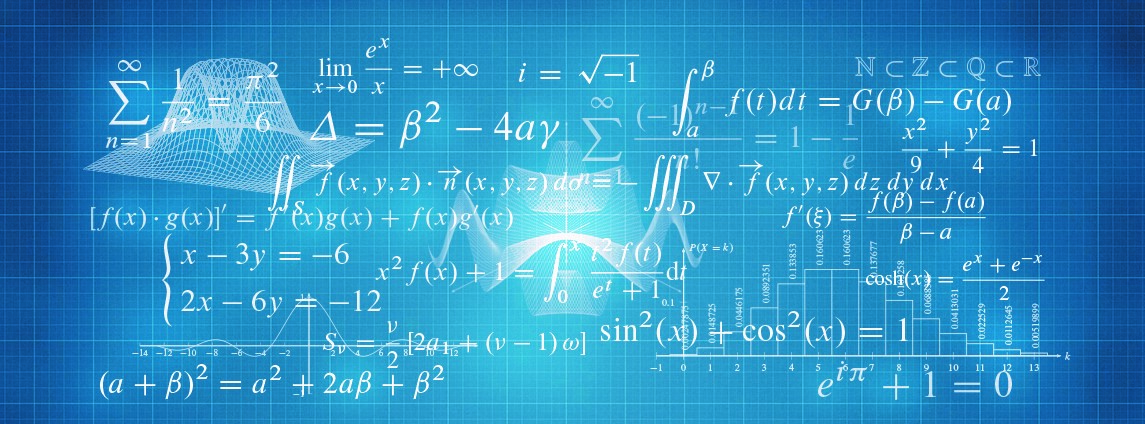
\includegraphics[width=17cm]{Kefalaio}};
\node[anchor=west,xshift=.12\paperwidth,yshift=.17\paperheight,rectangle]
{{\color{white}\fontsize{30}{20}\textbf{\textcolor{black}{\contour{white}{ΚΕΦΑΛΑΙΟ}}}}};
\node[anchor=west,xshift=.11\paperwidth,yshift=.11\paperheight,rectangle] {\fontsize{27}{20} {\color{black}{{\textcolor{black}{\contour{white}{\sc##1}}}}}};
%\fill[fill=black] (12.2,2) rectangle (14.8,4.7);
\node[anchor=west,xshift=.74\paperwidth,yshift=.14\paperheight,rectangle]
{{\color{white}\fontsize{80}{20}\textbf{\textit{\textcolor{white}{\contour{black}{\thechapter}}}}}};
\end{tikzpicture}
};
\end{tikzpicture}
}
\titlespacing*{\chapter}{0pt}{20pt}{30pt}
}
%------------------------------------------------


\usepackage[outline]{contour}
\newcommand{\regularchapter}{%
\titleformat{\chapter}[display]
{\normalfont\huge\bfseries}{\chaptertitlename\ \thechapter}{20pt}{\Huge##1}
\titlespacing*{\chapter}
{0pt}{-20pt}{40pt}
}

\apptocmd{\mainmatter}{\fancychapter}{}{}
\apptocmd{\backmatter}{\regularchapter}{}{}
\apptocmd{\frontmatter}{\regularchapter}{}{}

\titlespacing*{\section}
{0pt}{30pt}{0pt}
\usepackage{booktabs}
\usepackage{hhline}
\DeclareRobustCommand{\perthousand}{%
\ifmmode
\text{\textperthousand}%
\else
\textperthousand
\fi}

\newcounter{typos}[chapter]
\renewcommand{\thetypos}{T\arabic{typos}}   
\newcommand{\Typos}{\refstepcounter{typos}\textcolor{gray}{\textbf{\thetypos}}}{}


\contentsmargin{0cm}
\titlecontents{part}[-1pc]
{\addvspace{10pt}%
\bf\Large ΜΕΡΟΣ\quad }%
{}
{}
{\;\dotfill\;\normalsize\ Σελίδα}%
%------------------------------------------
\titlecontents{chapter}[0pc]
{\addvspace{30pt}%
\begin{tikzpicture}[remember picture, overlay]%
\draw[fill=black,draw=black] (-.3,.5) rectangle (3.7,1.1); %
\pgftext[left,x=0cm,y=0.75cm]{\color{white}\sc\Large\bfseries Κεφάλαιο\ \thecontentslabel};%
\end{tikzpicture}\large\sc}%
{}
{}
{\hspace*{-2.3em}\hfill\normalsize Σελίδα \thecontentspage}%
\titlecontents{section}[2.4pc]
{\addvspace{1pt}}
{\contentslabel[\thecontentslabel]{2pc}}
{}
{\;\dotfill\;\small \thecontentspage}
[]
\titlecontents*{subsection}[4pc]
{\addvspace{-1pt}\small}
{}
{}
{\ --- \small\thecontentspage}
[ \textbullet\ ][]

\makeatletter
\renewcommand{\tableofcontents}{%
\chapter*{%
\vspace*{-20\p@}%
\begin{tikzpicture}[remember picture, overlay]%
\pgftext[right,x=12cm,y=0.2cm]{\Huge\sc\bfseries \contentsname};%
\draw[fill=black,draw=black] (9.5,-.75) rectangle (12.5,1);%
\clip (9.5,-.75) rectangle (15,1);
\pgftext[right,x=12cm,y=0.2cm]{\color{white}\Huge\bfseries \contentsname};%
\end{tikzpicture}}%
\@starttoc{toc}}
\makeatother

\usepackage[contents={},scale=1,opacity=1,color=black,angle=0]{background}

\newcommand\blfootnote[1]{%
\begingroup
\renewcommand\thefootnote{}\footnote{#1}%
\addtocounter{footnote}{-1}%
\endgroup
}
\usepackage{epstopdf}
\epstopdfsetup{update}
\usepackage{textcomp}
\titleformat{\section}
{\normalfont\Large\bf}%
{}{0em}%
{{\color{black}\titlerule[1pt]}\vskip-.2\baselineskip{\parbox[t]{\dimexpr\textwidth-2\fboxsep\relax}{\raggedright\strut\thesection~#1\strut}}}[\vskip 0\baselineskip{\color{black}\titlerule[1pt]}]
\titlespacing*{\section}{0pt}{0pt}{0pt}

\newcommand{\methodologia}{\begin{center}
{\large \textbf{\textcolor{cyan}{ΜΕΘΟΔΟΛΟΓΙΑ}}}\\\vspace{-2mm}
\begin{tikzpicture}
\shade[left color=white, right color=cyan] (-3cm,0) rectangle (0,.2mm);
\shade[left color=cyan, right color=white] (0,0) rectangle (3cm,.2mm);   
\end{tikzpicture}
\end{center}}

\newcommand{\orismoi}{\begin{center}
\large \textbf{\textcolor{cyan}{ΟΡΙΣΜΟΙ}}\\\vspace{-2mm}
\begin{tikzpicture}
\shade[left color=white, right color=cyan] (-3cm,0) rectangle (0,.2mm);
\shade[left color=cyan, right color=white] (0,0) rectangle (3cm,.2mm);   
\end{tikzpicture}
\end{center}}
\newcommand{\thewrhmata}{\begin{center}
{\large \textbf{\textcolor{cyan}{ΘΕΩΡΗΜΑΤΑ - ΠΟΡΙΣΜΑΤΑ - ΠΡΟΤΑΣΕΙΣ\\ΚΡΙΤΗΡΙΑ - ΙΔΙΟΤΗΤΕΣ}}}\\\vspace{-2mm}
\begin{tikzpicture}
\shade[left color=white, right color=cyan] (-3cm,0) rectangle (0,.2mm);
\shade[left color=cyan, right color=white] (0,0) rectangle (3cm,.2mm);   
\end{tikzpicture}
\end{center}}
\usepackage[labelfont={footnotesize,it,bf},font={footnotesize}]{caption}
\usepackage{systeme,regexpatch}
\makeatletter
% change the definition of \sysdelim not to store `\left` and `\right`
\def\sysdelim#1#2{\def\SYS@delim@left{#1}\def\SYS@delim@right{#2}}
\sysdelim\{. % reinitialize
% patch the internal command to use
% \LEFTRIGHT<left delim><right delim>{<system>}
% instead of \left<left delim<system>\right<right delim>
\regexpatchcmd\SYS@systeme@iii
{\cB.\c{SYS@delim@left}(.*)\c{SYS@delim@right}\cE.}
{\c{SYS@MT@LEFTRIGHT}\cB\{\1\cE\}}
{}{}
\def\SYS@MT@LEFTRIGHT{%
\expandafter\expandafter\expandafter\LEFTRIGHT
\expandafter\SYS@delim@left\SYS@delim@right}
\makeatother
\newcommand{\synt}[2]{{\scriptsize \begin{matrix}
\times#1\\\\ \times#2
\end{matrix}}}
%----------------------------------------
\usepackage{wrapfig}
%-------- ΜΑΘΗΜΑΤΙΚΑ ΕΡΓΑΛΕΙΑ ---------
\usepackage{mathtools}
%----------------------
%-------- ΠΙΝΑΚΕΣ ---------
\usepackage{booktabs}
%----------------------
%----- ΥΠΟΛΟΓΙΣΤΗΣ ----------
%\usepackage{calculator}
%----------------------------
%--------- ΑΝΙΣΩΣΕΙΣ -------
\tikzset{
thickest/.style={line width=1mm},a/.style={decoration={markings,
mark=at position #1 with {\fill[white,draw=cyan,thin] circle (3pt);}},postaction={decorate}},
k/.style={decoration={markings,
mark=at position #1 with {\fill[black] circle (3pt);}},postaction={decorate}},
}
%--------- ΔΙΑΣΤΗΜΑ ------------
\newcommand{\diasthma}[7]{
\foreach \x in {#3,#4}
\draw (\x,#7+.2) -- (\x,#7-.2);
\node[anchor=north,fill=white] at (#3,#7)[below=1mm] {$ #1 $};
\node[anchor=north,fill=white] at (#4,#7)[below=1mm] {$ #2 $};
\draw [#5=0,#6=1,thickest] (#3,#7)--(#4,#7);
}
%--------- ΑΞΟΝΑΣ ------------------
\newcommand{\axonas}[3]{
\draw[-latex] (#1,#3) -- (#2,#3)node[right]{$x$};
}
%--------- ΚΑΤΩ ΑΚΡΟ ------------------
\newcommand{\Xapeiro}[5]{
\draw (#2,#5+.2) -- (#2,#5-.2);
\node[anchor=north,fill=white] at (#2,#5)[below=1mm] {$ #1 $};
\draw [#4=0,thickest] (#2,#5)--(#3-.3,#5);
}
%--------- ΠΑΝΩ ΑΚΡΟ ------------------
\newcommand{\apeiroX}[5]{
\draw (#2,#5+.2) -- (#2,#5-.2);
\node[anchor=north,fill=white] at (#2,#5)[below=1mm] {$ #1 $};
\draw [#4=0,thickest] (#2,#5)--(#3+.3,#5);
}
%----- ΔΙΑΚΕΚΟΜΜΕΝΕΣ ΓΡΑΜΜΕΣ ------
\newcommand{\oria}[3]{\draw [dashed] (#1,#2)--(#1,#3);}
%--------------------------------------
%----- ΟΡΙΖΟΝΤΙΑ ΛΙΣΤΑ ------
\usepackage{xparse}
\newcounter{answers}
\renewcommand\theanswers{\arabic{answers}}
\ExplSyntaxOn
\NewDocumentCommand{\results}{m}
{
\seq_set_split:Nnn \l_results_a_seq {,}{#1}
\par\nobreak\noindent\setcounter{answers}{0}
\seq_map_inline:Nn \l_results_a_seq
{
\makebox[.18\linewidth][l]{\stepcounter{answers}\theanswers.~##1}\hfill
}
\par
}
\seq_new:N \l_results_a_seq
\ExplSyntaxOff
%----------------------------
%------ ΜΗΚΟΣ ΓΡΑΜΜΗΣ ΚΛΑΣΜΑΤΟΣ ---------
\DeclareRobustCommand{\frac}[3][0pt]{%
{\begingroup\hspace{#1}#2\hspace{#1}\endgroup\over\hspace{#1}#3\hspace{#1}}}
%----------------------------------------
\usepackage{microtype}
\usepackage{float}
\newcommand{\hm}[1]{\textrm{ημ}#1}
\newcommand{\syn}[1]{\textrm{συν}#1}
\newcommand{\ef}[1]{\textrm{εφ}#1}
\newcommand{\syf}[1]{\textrm{σφ}#1}
\usepackage{caption}
%----------- ΓΡΑΦΙΚΕΣ ΠΑΡΑΣΤΑΣΕΙΣ ---------
\pgfkeys{/pgfplots/aks_on/.style={axis lines=center,
xlabel style={at={(current axis.right of origin)},xshift=1.5ex, anchor=center},
ylabel style={at={(current axis.above origin)},yshift=1.5ex, anchor=center}}}
\pgfkeys{/pgfplots/grafikh parastash/.style={cyan,line width=.4mm,samples=200}}
\pgfkeys{/pgfplots/belh ar/.style={tick label style={font=\scriptsize},axis line style={-latex}}}
%-----------------------------------------
%--------- ΟΡΙΣΜΑ --------------
\newcommand{\Arg}[9]{
\draw[-latex] (#7,#8)-- ++(#1:#2) node[#9=#5]{\footnotesize$#4$};
\draw[fill=black!#6] (#7+0.3+#3,#8) arc (0:#1:0.3+#3) -- (#7,#8);}
%-------------------------------
%---- ΟΡΙΖΟΝΤΙΟ - ΚΑΤΑΚΟΡΥΦΟ - ΠΛΑΓΙΟ ΑΓΚΙΣΤΡΟ ------
\newcommand{\orag}[3]{\node at (#1)
{$ \overcbrace{\rule{#2mm}{0mm}}^{{\scriptsize #3}} $};}

\newcommand{\kag}[3]{\node at (#1)
{$ \undercbrace{\rule{#2mm}{0mm}}_{{\scriptsize #3}} $};}

\newcommand{\Pag}[4]{\node[rotate=#1] at (#2)
{$ \overcbrace{\rule{#3mm}{0mm}}^{{\rotatebox{-#1}{\scriptsize$#4$}}}$};}
%-----------------------------------------
\tikzstyle{pl}=[line width=0.3mm]
\tikzstyle{plm}=[line width=0.4mm]
\tkzSetUpPoint[size=7,fill=white]
\newlist{rlist}{enumerate}{3}
\setlist[rlist]{itemsep=0mm,label=\roman*.}
\newcolumntype{C}{>{\centering\arraybackslash} X}
\setlist[itemize]{itemsep=0mm}
\makeatletter
\def\closedcycley{%
-| (perpendicular cs: 
horizontal line through={(current plot begin)}, 
vertical line through={(\pgfplots@ZERO@x,\pgfplots@ZERO@y)})
-- cycle
}%
\makeatother
\newcommand{\tss}[1]{\textsuperscript{#1}}
\newcommand{\tssL}[1]{\MakeLowercase\textsuperscript{#1}}
\newcommand{\eis}[1]{\textquotedblleft#1\textquotedblright\;}
%------ ΔΙΑΓΩΝΙΟ ΣΕ ΠΙΝΑΚΑ -------
\usepackage{array}
\newcommand\diag[5]{%
\multicolumn{1}{|m{#2}|}{\hskip-\tabcolsep
$\vcenter{\begin{tikzpicture}[baseline=0,anchor=south west,outer sep=0]
\path[use as bounding box] (0,0) rectangle (#2+2\tabcolsep,\baselineskip);
\node[minimum width={#2+2\tabcolsep-\pgflinewidth},
minimum  height=\baselineskip+#3-\pgflinewidth] (box) {};
\draw[line cap=round] (box.north west) -- (box.south east);
\node[anchor=south west,align=left,inner sep=#1] at (box.south west) {#4};
\node[anchor=north east,align=right,inner sep=#1] at (box.north east) {#5};
\end{tikzpicture}}\rule{0pt}{.71\baselineskip+#3-\pgflinewidth}$\hskip-\tabcolsep}}
%---------------------------------


\begin{document}
\title{\MakeUppercase{ΣΧΟΛΙΚΟ ΤΥΠΟΛΟΓΙΟ}}
\pagestyle{empty}
\frontmatter
\begin{titlepage}
\newgeometry{left=2.5cm,top=2.5cm} %defines the geometry for the titlepage
\pagecolor{white}
\begin{center}
{\large Σπύρος Φρόνιμος\\Μαθηματικός}
\end{center}
\noindent
\par
\noindent
\mbox{}\\\\
\begin{center}
\textbf{\fontsize{25}{40}\selectfont{ΜΑΘΗΜΑΤΙΚΟ ΤΥΠΟΛΟΓΙΟ}}\par\mbox{}\\
{\fontsize{20}{30}\selectfont \MakeUppercase{\textbf{ΓΥΜΝΑΣΙΟΥ - ΛΥΚΕΙΟΥ}}}\\
\vspace{7mm}
{\fontsize{15}{15}\selectfont \sc{τύποι ορισμοί θεωρήματα και}}\\
\vspace{.7mm}
{\fontsize{15}{15}\selectfont \sc{βασική μεθοδολογία των μαθηματικων}}

\end{center}
\vspace{1.5cm}
\[ f(x)= \frac{\eta\mu x}{x}\]
\vspace{-5mm}
\begin{center}
\begin{tikzpicture}[domain=-3*pi:3*pi,x=0.6cm,y=4.4cm]
\tkzInit[xmin=-10,xmax=10,ymin=-.5,ymax=1.2,ystep=1]
\draw[-latex] (-10,0) -- coordinate (x axis mid) (10,0) node[right,fill=white] {{\footnotesize $ x $}};
\draw[-latex] (0,-.5) -- (0,1.2) node[above,fill=white] {{\footnotesize $ y $}};
\foreach \y in {-0.4,-0.2,0,0.2,0.4,0.6,0.8,1}
\draw (.5mm,\y) -- (-.5mm,\y) node[anchor=east,fill=white] {{\scriptsize \y}};
\foreach \x in {-9,-8,...,9}
\draw (\x,.5mm) -- (\x,-.5mm) node[anchor=north,fill=white] {{\scriptsize \x}};
\draw[samples=150,line width=.5mm] plot function{sin(x)/x};
%\tkzText(3,0.8){$ f(x)=\dfrac{\eta\mu x}{x} $}
\end{tikzpicture}
\end{center}

\vfill
\noindent
\color{black}
\begin{center}
{\large{ΕΚΔΟΣΕΙΣ \_\_\_\_\_}\\
\large{ΚΕΡΚΥΡΑ 2015}}
\vskip\baselineskip
\end{center}
\hbox{ % Horizontal box
\hspace*{0.2\textwidth} % Whitespace to the left of the title page
\rule{1pt}{\textheight} % Vertical line
\hspace*{0.05\textwidth} % Whitespace between the vertical line and title page text
\parbox[b]{0.75\textwidth}{ % Paragraph box which restricts text to less than the width of the page

{\textbf{ΜΑΘΗΜΑΤΙΚΟ ΤΥΠΟΛΟΓΙΟ}\\\textbf{Γυμνασίου - Λυκείου}\\\\\noindent \textbf{Σπύρος Φρόνιμος - Μαθηματικός}\\e-mail : spyrosfronimos@gmail.com}\\[0.5\baselineskip]
Σελίδες : ...\\
ΙΣΒΝ : ...\\
Εκδόσεις : ...\\
\textcopyright Copyright 2015\\[2\baselineskip] % Title
{Φιλολογική Επιμέλεια :\\\textbf{Μαρία Πρεντουλή}}
{- e-mail : predouli@yahoo.com}\\[0.5\baselineskip]
{Επιστημονική Επιμέλεια :}\\
{\textbf{Ιωάννα Γραμμένου - }}{ - e-mail : predouli@yahoo.com}\\{\textbf{Σπύρος Φρόνιμος}}\\[0.5\baselineskip]
{Εξώφυλλο : \\\textbf{Δημήτρης Πρεντουλής}}\\[1\baselineskip] % Tagline or further description
% Author name

\vspace{.4\textheight} % Whitespace between the title block and the publisher
{Πνευματικά Δικαιώματα : ...}\\[\baselineskip]}}
\vspace*{2\baselineskip}
\newpage
\mbox{}\\\\\\\\\\\\
\hspace*{0.75\textwidth}
\textit{{\large Στους γονείς μου.}}
\newpage
\mbox{}
\newpage
\mbox{}
{\LARGE \textbf{Πρόλογος}}\\\\\\\\

Το βιβλίο περιέχει συγκεντρωμένη όλη τη θεωρία των μαθηματικών όλων των τάξεων του γυμνασίου και του λυκείου γραμμένη αναλυτικά και κατανοητά.\\\\
Ειδικότερα ο αναγνώστης θα βρει\\
\vspace{-.4cm}
\begin{itemize}
\item Ορισμούς
\item Θεωρήματα
\item Τυπολόγιο
\item Μεθοδολογία
\end{itemize}
Σκοπό έχει να αποτελέσει ένα χρήσιμο βοήθημα για μικρούς ή μεγάλους μαθητές όπου μπορούν να έχουν όλη τη θεωρία της χρονιάς τους συγκεντρωμένη, χρήσιμη για επανάληψη και διαγωνίσματα, αλλά και να μπορούν εύκολα να καλύψουν τυχόν κενά από προηγούμενες τάξεις.\\\\\\
Θέλω να ευχαριστήσω όλους όσους βοήθησαν.
\newpage
\end{titlepage}
\restoregeometry % restores the geometry

\tableofcontents
\newpage
\noindent
\newcolumntype{C}{>{\centering\arraybackslash}m{7cm} }
\chapter*{Πίνακας Συμβόλων}
\addtocontents{toc}{{\sc{\large Πίνακας Συμβόλων}}\dotfill\thepage\\\\}
{\par\centering

\begin{tabularx}{\textwidth}{c>{\centering}m{3.1cm}C}
\hline\rule[-2ex]{0pt}{5.5ex}\textbf{Σύμβολο} & \textbf{Όνομα} & \textbf{Περιγραφή}\\
\hhline{===}\rule[-2ex]{0pt}{8.5ex}
$ +\;,\; -\;,\; \cdot\;,\; : $ &  Συν, Πλην, Επί, Δια & Τα σύμβολα της πρόσθεσης, της αφαίρεσης, του πολλαπλασιασμού και της διαίρεσης αντίστοιχα.\\
\rule[-2ex]{0pt}{5.5ex}
$ = $ & Ίσον & Δηλώνει ισότητα ανάμεσα σε δύο στοιχεία.\\
\rule[-2ex]{0pt}{5.5ex}
$ \equiv $ & Ταυτίζεται & \\
\rule[-2ex]{0pt}{5.5ex}
$ \neq $ & Διάφορο & Εκφράζει οτι δύο στοιχεία είναι διαφορετικά μεταξύ τους.\\
\rule[-2ex]{0pt}{5.5ex}
$ > $ & Μεγαλύτερο & Δηλώνει ανισότητα ανάμεσα σε δύο στοιχεία. (Το 1\textsuperscript{ο} μεγαλύτερο του 2\textsuperscript{ου}).\\
\rule[-2ex]{0pt}{5.5ex}
$ < $ & Μικρότερο & Δηλώνει ανισότητα ανάμεσα σε δύο στοιχεία. (Το 1\textsuperscript{ο} μικρότερο του 2\textsuperscript{ου}).\\
\rule[-2ex]{0pt}{5.5ex}
$ \geq $ & Μικρότερο ίσο & Συνδυασμός των σχέσεων $=$ και $>$.\\
\rule[-2ex]{0pt}{5.5ex}
$ \leq $ & Μικρότερο ίσο & Συνδυασμός των σχέσεων $=$ και $<$.\\
\rule[-2ex]{0pt}{5.5ex}
$ \pm $ & Συν Πλην & Συνδυασμός των προσήμων $+$ και $-$.\\
\rule[-2ex]{0pt}{5.5ex}
$ \mp $ & Πλην Συν & Έχει την ίδια σημασία με το συμβολισμό $\pm$  και χρησιμοποιείται όταν θέλουμε να αλλάξουμε τη σειρά με την οποία θα εμφανιστούν τα πρόσημα $+\;,\;-$. \\
\rule[-2ex]{0pt}{7ex}
$ \Rightarrow $ & Συνεπαγωγή & Συνδέει δύο μαθηματικές προτάσεις, όταν η μια έχει σαν συμπέρασμα την άλλη. \\
\rule[-2ex]{0pt}{7ex}
$ \Leftarrow $ & Αντίστροφη συνεπαγωγή & Συνδέει δύο μαθηματικές προτάσεις με φορά αντίστροφη από το σύνδεσμο $ \Rightarrow $. \\
\rule[-2ex]{0pt}{7ex}
$ \Leftrightarrow $ & Διπλή συνεπαγωγή & Συνδέει δύο μαθηματικές προτάσεις με διπλή φορά. Δηλώνει ισοδυναμία μεταξύ τους.  \\
\rule[-2ex]{0pt}{7ex}
$ \% $ & Ποσοστό τοις εκατό & Μέρος μιας ποσότητας μοιρασμένης σε 100 ίσα κομμάτια. \\
\rule[-2ex]{0pt}{7ex}
$ \perthousand $ & Ποσοστό τοις χιλίοις & Μέρος μιας ποσότητας μοιρασμένης σε 1000 ίσα κομμάτια. \\
\hline
\end{tabularx}
\par}
\newpage
\noindent
{\par\centering
\begin{tabularx}{\textwidth}{c>{\centering}m{3.1cm}>{\centering\arraybackslash}m{7.75cm}}
\hline\rule[-2ex]{0pt}{5.5ex}\textbf{Σύμβολο} & \textbf{Όνομα} & \textbf{Περιγραφή}\\
\hhline{===}\rule[-2ex]{0pt}{8.5ex}
$ |\;\;| $ & Απόλυτη τιμή & Απόσταση ενός αριθμού από το 0. \\
\rule[-2ex]{0pt}{5.5ex}
$ \sqrt{\;\;} $ & Τετραγωνική ρίζα & Βλ. \textbf{Ορισμό ...} \\
\rule[-2ex]{0pt}{5.5ex}
$ \sqrt[\nu]{\;\;} $ & ν-οστή ρίζα & Βλ. \textbf{Ορισμό ...} \\
\rule[-2ex]{0pt}{7.5ex}
$ \in $ & Ανήκει & Σύμβολο το οποίο δηλώνει οτι ένα στοιχείο ανήκει σε ένα σύνολο. \\
\rule[-2ex]{0pt}{7.5ex}
$ \ni $ & Ανήκει & Έχει την ίδια χρησμότητα με το σύμβολο $ \in $ και χρησιμοποιείται όταν θέλουμε να γράψουμε το όνομα του συνόλου πριν από το όνομα του στοιχείου. \\
\rule[-2ex]{0pt}{7.5ex}
$ \notin $ & Δεν ανήκει & Έχει την αντίθετη σημασία από το σύμβολο $ \in $ και δηλώνει οτι ένα στοιχείο δεν ανήκει σε ένα σύνολο. \\
\rule[-2ex]{0pt}{5.5ex}
$ \subseteq $ & Υποσύνολο & Βλ. \textbf{Ορισμό ...} \\
\rule[-2ex]{0pt}{5.5ex}
$ \supseteq $ & Υπερσύνολο & \\
\rule[-2ex]{0pt}{5.5ex}
$ \subset\;,\;\supset $ & Γνήσιο υποσύνολο, γν. υπερσύνολο & \\
\rule[-2ex]{0pt}{5.5ex}
$ \cup\;,\;\cap $ & Ένωση, Τομή & Βλ. \textbf{Ορισμό ...} \\
\rule[-2ex]{0pt}{5.5ex}
$ \varnothing $ & Κενό σύνολο & Βλ. \textbf{Ορισμό ...} \\
\rule[-2ex]{0pt}{5.5ex}
$ \infty $ & Άπειρο & \\
\rule[-2ex]{0pt}{5.5ex}
$ \forall $ & Για κάθε & Βλ. \textbf{Ορισμό ...} \\
\rule[-2ex]{0pt}{5.5ex}
$ \exists $ & Υπάρχει & Βλ. \textbf{Ορισμό ...} \\
\rule[-2ex]{0pt}{5.5ex}
$ \nexists $ & Δεν υπάρχει & \\	
\rule[-2ex]{0pt}{5.5ex}
$ \bot $ & Κάθετο & \\
\rule[-2ex]{0pt}{5.5ex}
$ \sum $ & Άθροισμα & \\
\rule[-2ex]{0pt}{5.5ex}
$ \prod $ & Γινόμενο & \\
\rule[-2ex]{0pt}{5.5ex}
$ \displaystyle\int $ & Ολοκλήρωμα & Βλ. \textbf{Ορισμό ...} \\
\hline
\end{tabularx}
\par}
\newpage
\noindent
{\par\centering
\begin{tabularx}{\textwidth}{c>{\centering}m{3.1cm}C}
\hline\rule[-2ex]{0pt}{5.5ex}\textbf{Σύμβολο} & \textbf{Όνομα} & \textbf{Περιγραφή}\\
\hhline{===}\rule[-2ex]{0pt}{5.5ex}
$ \lim $ & Όριο & Βλ. \textbf{Ορισμό ...} \\
\rule[-2ex]{0pt}{5.5ex}
$ \log, \ln $ & Λογάριθμός & Βλ. \textbf{Ορισμό ...} \\
\rule[-2ex]{0pt}{8.5ex}
$ \displaystyle\binom{\nu}{\kappa} $ & Διωνυμικός συντελεστής &  \\
\hline
\end{tabularx}
\par}
\chapter*{Βασικές Έννοιες}
\addtocontents{toc}{\sc {\large Βασικες Έννοιες}\dotfill\thepage}
Η επιστήμη των μαθηματικών
\begin{enumerate}[label=\large{\bf Α-\arabic*.}]
\item \textbf{\MakeUppercase Άλγεβρα}\\
\item \textbf{\MakeUppercase Γεωμετρία}\\
\item \textbf{\MakeUppercase Στατιστική}\\
\item \textbf{\MakeUppercase Πιθανότητες}\\
\item \textbf{\MakeUppercase Ανάλυση}\\
\item \textbf{\MakeUppercase Εφαρμοσμένα μαθηματικά}\\
\end{enumerate}

Πριν δούμε αναλυτικά τους ορισμούς, τους κανόνες και τις βασικές μεθόδους της θεωρίας των μαθηματικών θα πρέπει να ερμηνεύσουμε αυτές τις βασικές έννοιες καθώς και κάθε έννοια που προκύπτει μέσα απ\textquoteright αυτές ή είναι χρήσιμη για τη δομή ενός μαθηματικού κειμένου.
\begin{enumerate}[label=\large{\bf B-\arabic*.}]
\item \textbf{ΟΡΙΣΜΟΣ}\\
Ορισμός ονομάζεται μια πρόταση η οποία εισάγει και ερμηνεύει πλήρως μια νέα μαθηματική έννοια, με τρόπο σαφή και σύντομο.
\item \textbf{ΘΕΩΡΗΜΑ}\\
Θεώρημα καλείται κάθε πρόταση η οποία αποτελεί ένα βασικό και αποδεδειγμένο κανόνα μεταξύ μαθηματικών εννοιών. \begin{itemize}[itemsep=0mm]
\item Αποτελείται από δύο μέρη τα οποία είναι μαθηματικές προτάσεις και ονομάζονται \textbf{υπόθεση} και \textbf{συμπέρασμα}.
\item Η υπόθεση αποτελείται από μια ή περισσότερες προτάσεις οι οποίες είναι αναγκαίες για να οδηγηθούμε στο συμπέρασμα το οποίο είναι λογική συνέπεια αυτών.
\item Η ισχύς ενός θεωρήματος είναι γενική. Μαθηματικές προτάσεις με μικρότερη βαρύτητα αποτελούν υποκατηγορίες της έννοιας του θεωρήματος. Αυτές είναι τα πορίσματα, οι προτάσεις, τα κριτήρια και οι ιδιότητες.
\end{itemize}
\item \textbf{Πόρισμα}\\
Πόρισμα λέγεται μια πρόταση η οποία προκυπτει άμεσα από ένα θεώρημα και αποδεικνύεται με τη βοήθεια αυτού. Είναι ένας κανόνας με συμπέρασμα πιο είδικό απ\textquoteright αυτό ενός θεωρήματος.
\item \textbf{Κριτήριο}\\
Κριτήριο ονομάζεται μια πρόταση η οποία αποτελεί έναν κανόνα με τον οποίο ελέχεται η ισχύς μιας ιδιότητας ή ενός χαρακτηριστικού. Αν ικανοποιούνται οι συνθήκες ενός κριτηρίου τότε ως συμπέρασμα έχουμε τη ζητούμενη ιδιότητα ή χαρακτηριστικό ενός μαθηματικού αντικειμένου.
\item \textbf{Ιδιότητα}\\
\item \textbf{Χαρακτηριστικό}\\
\item \textbf{Παράδειγμα}\\
\item \textbf{Αντιπαράδειγμα}\\
\item \textbf{Αξίωμα}\\
\item \textbf{Γεωμετρική ερμηνεία}\\
\item \textbf{Διερεύνηση}\\
\item \textbf{Ισχυρισμός}\\
\item \textbf{Περιορισμός}\\
\item \textbf{Παρατήρηση}\\
\item \textbf{Σχόλιο}\\
\item \textbf{Γενίκευση}\\
\item \textbf{Εικασία}\\
\item \textbf{Ιδιότητα}\\
\end{enumerate}
\mainmatter
\pagestyle{fancy}
\chapter{Άλγεβρα}
\section{Αριθμοί}\mbox{}\\
\orismoi
\Orismos{Bασικα Συνολα Aριθμων}
\vspace{-5mm}
\begin{enumerate}[itemsep=0mm,label=\bf\arabic*.]
\item \textbf{Φυσικοί Αριθμοί}\Algebra{Φυσικοί αριθμοί} : Το σύνολο των αριθμών από το 0 εως το άπειρο όπου κάθε αριθμός έχει διαφορά μιας μονάδας από τον προηγούμενο. Συμβολίζεται με $ \mathbb{N} $ και είναι : $ \mathbb{N}=\{0,1,2,\ldots\} $.
\item \textbf{Ακέραιοι Αριθμοί}\Algebra{Ακέραιοι αριθμοί} : Το σύνολο των φυσικών αριθμών μαζί με τους αντίθετους τους. Συμβολίζεται με $ \mathbb{Z} $ και είναι : $ \mathbb{Z}=\{\ldots,-2,-1,0,1,2,\ldots\} $.
\item \textbf{Ρητοί Αριθμοί}\Algebra{Ρητοί αριθμοί} : Όλοι οι αριθμοί που μπορούν να γραφτούν με τη μορφή κλάσματος με ακέραιους όρους. Συμβολίζεται με $ \mathbb{Q} $ και είναι : $ \mathbb{Q}=\LEFTRIGHT\{\}{\left. \frac{a}{\beta}\right|a,\beta\in\mathbb{Z},\beta\neq0\;} $.
\item \textbf{Άρρητοι Αριθμοί}\Algebra{Άρρητοι αριθμοί} : Κάθε αριθμός ο οποίος δεν είναι ρητός. Κατά κύριο λόγο, άρρητοι αριθμοί είναι οι ρίζες που δεν έχουν ρητό αποτέλεσμα, ο αριθμός $ \pi $ κ.τ.λ.
\item \textbf{Πραγματικοί Αριθμοί}\Algebra{Πραγματικοί αριθμοί} : Οι ρητοί μαζί με το σύνολο των άρρητων μας δίνουν τους πραγματικούς αριθμούς, όλους τους αριθμούς που γνωρίζουμε. Συμβολίζεται με $ \mathbb{R} $ και είναι : $ \mathbb{R}= $ $ \{ $όλοι οι αριθμοί$ \} $.
\item \textbf{Μιγαδικοί Αριθμοί} \Algebra{Μιγαδικοί αριθμοί} : Οι αριθμοί που αποτελούν άθροισμα ενός πραγματικού με ένα φανταστικό αριθμό. Οι αριθμοί είναι της μορφής $ a+\beta i $ ενώ το σύνολο των μιγαδικών αριθμών συμβολίζεται με $ \mathbb{C} $ και είναι $ \mathbb{C}=\{z=a+\beta i|a,\beta\in\mathbb{R}\textrm{ με }i^2=-1\} $.
\end{enumerate}
Τα παραπάνω σύνολα χωρίς το μηδενικό τους στοιχείο συμβολίζονται αντίστοιχα με $ \mathbb{N}^*,\mathbb{Z}^*,\\\mathbb{Q}^*,\mathbb{R}^*,\mathbb{C}^* $.\\
Με το σύνολο $ \mathbb{C} $ των μιγαδικών αριθμών θα ασχοληθούμε εκτενέστερα στην \textbf{Παράγραφο 1.5} όπου θα ορίσουμε κάθε έννοια, που αφορά το σύνολο αυτό, αναλυτικά.\\\\
\Orismos{δεκαδικο συστημα αρίθμησησ}\Algebra{Δεκαδικό σύστημα}Δεκαδικό ονομάζεται το σύστημα αρίθμησης στο οποίο κάθε αριθμός σχηματίζεται με τη χρήση των δέκα συμβόλων - ψηφίων : $ 0,1,2,3,4,5,6,7,8,9 $ τοποθετημένα διαδοχικά το ένα μετά το άλλο. Καθένα απ' αυτά έχει διαφορετική αξία ανάλογα με το πλήθος των μονάδων που εκφράζει. Στο δεκαδικό σύστημα έχουμε σαν βάση τον αριθμό δέκα.
\begin{center}
\begin{longtable}{c|>{\centering\arraybackslash}m{1.5cm}|>{\centering\arraybackslash}m{1.5cm}|>{\centering\arraybackslash}m{1.2cm}|>{\centering\arraybackslash}m{1cm}|>{\centering\arraybackslash}m{1.5cm}|>{\centering\arraybackslash}m{1cm}|>{\centering\arraybackslash}m{1cm}}
\hline  \multicolumn{8}{c}{\textbf{Ψηφία Ακέραιου Αριθμού}} \rule[-2ex]{0pt}{5.5ex}\\ 
\hhline{========} \rule[-2ex]{0pt}{6ex} \begin{minipage}{1.5cm}
\begin{center}
{\footnotesize \textbf{Δεκαδική}}\\{\footnotesize \textbf{Τάξη}}
\end{center}
\end{minipage} &
{\footnotesize Εκατομμύρια} & 
\begin{minipage}{1.5cm}
\begin{center}
\vspace{-1.4mm}
{\footnotesize Εκατοντάδες}\\{\footnotesize Χιλιάδες}
\end{center}
\end{minipage} & 
\begin{minipage}{1.3cm}
\begin{center}
{\footnotesize Δεκάδες}\\{\footnotesize Χιλιάδες}
\end{center}
\end{minipage} & 
{\footnotesize Χιλιάδες}& 
{\footnotesize Εκατοντάδες} & 
{\footnotesize Δεκάδες}& 
{\footnotesize Μονάδες}  \\ 
\hline \rule[-1.5ex]{0pt}{4.5ex} {\footnotesize \textbf{Συμβ.}} & {\footnotesize Εκ} & {\footnotesize ΕΧ} & {\footnotesize ΔΧ} & {\footnotesize Χ} & {\footnotesize Ε} & {\footnotesize Δ} & {\footnotesize Μ} \\ 
\hline \rule[-1.5ex]{0pt}{4.5ex} {\footnotesize \textbf{Αξία}} & {\footnotesize $ 1.000.000 $} & {\footnotesize $ 100.000 $} & {\footnotesize $ 10.000 $} & {\footnotesize $ 1.000 $} & {\footnotesize $ 100 $} & {\footnotesize $ 10 $} & {\footnotesize $ 1 $}\\
\hline 
\end{longtable}\captionof{table}{Ψηφία ακέραιου αριθμού}
\end{center}
\begin{itemize}[itemsep=0mm]
\item Κάθε αριθμός έχει διαφορετική αξία ανάλογα με τη θέση και την αξία των ψηφίων που τον αποτελούν.
\item Σε κάθε αριθμό η θέση κάθε ψηφίου καθορίζει την αξία του. Η θέση αυτή ονομάζεται \textbf{δεκαδική θέση}.
\item Η αξία των δεκαδικών θέσεων αυξάνεται από τα δεξιά προς τα αριστερά.
\item Κάθε δεκαδική θεση έχει αξία δεκαπλάσια της προηγούμενης.
\end{itemize}
\Orismos{Άρτιοι - περιττοι αριθμοί}\Algebra{Άρτιος - περιττός αριθμός}\Algebra{Περιττός αριθμός}
Άρτιοι (ζυγοί) ονομάζονται οι αριθμοί που διαιρούνται με το $ 2 $ ενώ περιττοί (μονοί) όσοι δεν διαιρούνται με το $ 2 $. Η μορφή που έχουν αντίστοιχα είναι: 
\[ \textrm{Άρτιοι : }a=2\kappa\;\;,\;\;\textrm{Περιττοί : }a=2\kappa+1\;\;,\;\;\textrm{ όπου }\kappa\in\mathbb{Z} \]
Το τελευταίο ψηφίο κάθε άρτιου αριθμού είναι ένα από τα $ 0,2,4,6,8 $ ενώ ένας περιττός αριθμός τελείώνει σε ένα από τα $ 1,3,5,7,9 $.\\\\
\Orismos{θετικοσ - αρνητικοσ αριθμοσ}\Algebra{Θετικός αριθμός}\Algebra{Αρνητικός αριθμός}
Θετικός ονομάζεται κάθε αριθμός που είναι μεγαλύτερος του μηδενός ενώ αρνητικός ονομάζεται κάθε αριθμός που είναι μικρότερος του μηδενός.
\begin{itemize}[itemsep=0mm]
\item Τα σύμβολα $ + $ και $ - $ τα οποία χρησιμοποιούμε για να δείξουμε αν κάποιος αριθμός είναι θετικός ή αρνητικός ονομάζονται \textbf{πρόσημα}\Algebra{Πρόσημα}.
\item Το 0 δεν έχει πρόσημο.
\item Δύο αριθμοί με το ίδιο πρόσημο ονομάζονται \textbf{ομόσημοι}\Algebra{Ομόσημοι}.
\item Δύο αριθμοί με το διαφορετικά πρόσημα ονομάζονται \textbf{ετερόσημοι}\Algebra{Ετερόσημοι}.
\item Το 0 είναι μικρότερο από κάθε θετικό και μεγαλύτερο από κάθε αρνητικό αριθμό.
\item Κάθε θετικός αριθμός είναι μεγαλύτερος από κάθε αρνητικό αριθμό.
\item Ανάμεσα σε δύο αρνητικούς αριθμούς, μεγαλύτερος είναι εκείνος με τη μικρότερη απόλυτη τιμή.
\end{itemize}
\Orismos{Αντίθετοι αριθμοι}\Algebra{Αντίθετοι αριθμοί}
Αντίθετοι ονομάζονται οι αριθμοί που έχουν ίσες απόλυτες τιμές και αντίθετα πρόσημα. \[ \textrm{Ο αντίθετος ενός αριθμού }x\textrm{ είναι ο}-x \]
\Orismos{Πράξεισ αριθμών}
Στον παρακάτω πίνακα φαίνονται τα ονόματα των αριθμών που αποτελούν μια πράξη, τα ονόματα των αποτελεσμάτων και ο συμβολισμός κάθε πράξης.
\begin{center}
\begin{tabular}{cccc}
\hline \rule[-2ex]{0pt}{5.5ex} \textbf{Πράξη} & \textbf{Όροι} & \textbf{Αποτέλεσμα} & \textbf{Συμβολισμός} \\ 
\hhline{====} \rule[-2ex]{0pt}{5.5ex} \textbf{Πρόσθεση} & Προσθετέοι & Άθροισμα & $ a+\beta $ \\ 
\rule[-2ex]{0pt}{5.5ex} \textbf{Αφαίρεση} & Μειωτέος - Αφαιρετέος & Διαφορά & $ a-\beta $ \\ 
\rule[-2ex]{0pt}{5.5ex} \textbf{Πολλαπλασιασμός} & Παράγοντες & Γινόμενο & $ a\cdot\beta $ \\ 
\rule[-2ex]{0pt}{5.5ex} \textbf{Διαίρεση} & Διαιρετέος - Διαιρέτης & Πηλίκο & $ a:\beta $ \\ 
\hline\end{tabular}\captionof{table}{Βασικές πράξεις}
\end{center}
\begin{enumerate}[itemsep=0mm,label=\bf\arabic*.]
\item \textbf{Πρόσθεση}\\ \Algebra{Πρόσθεση}\Algebra{Προσθετέοι}\Algebra{Άθροισμα}Πρόσθεση ονομάζεται η πράξη με την οποία μπορούμε από δύο αριθμούς $ a,\beta\in\mathbb{R} $ να υπολογίσουμε τον αριθμό $ a+\beta $ που ονομάζεται \textbf{άθροισμα}.
\item \textbf{Πολλαπλασιασμόσ}\\
\Algebra{Πολλαπλασιασμός}\Algebra{Παράγοντες}\Algebra{Γινόμενο}
Πολλαπλασιασμός ονομάζεται η πράξη με την οποία μπορούμε από δύο αριθμούς $ a,\beta\in\mathbb{R} $ να υπολογίσουμε τον αριθμό $ a\cdot\beta $ που ονομάζεται \textbf{γινόμενο}.
\item \textbf{Αφαίρεση - Διαίρεση}\\\Algebra{Αφαίρεση}\Algebra{Μειωτέος}\Algebra{Αφαιρετέος}\Algebra{Διαφορά}
Η αφαίρεση $ a-\beta $ και η διαίρεση $ a:\beta $ δύο αρθμών $ a,\beta\in\mathbb{R} $ είναι οι πράξεις που προκύπτουν από την πρόσθεση και τον πολλαπλασιασμό αντίστοιχα και μπορούν να γραφτούν με τη βοήθεια τους.
\[ a-\beta=a+(-\beta)\;\;,\;\;a:\beta=\frac{a}{\beta}=a\cdot\frac{1}{\beta} \]
\begin{itemize}[itemsep=0mm]
\item Το αποτέλεσμα της αφαίρεσης ονομάζεται \textbf{διαφορά} ενώ το αποτέλεσμα της διαίρεσης ονομάζεται \textbf{πηλίκο}.
\item Η διαίρεση ενός αριθμού $ a $ με το 0 \textbf{δεν} ορίζεται.
\item Η διαίρεση $0:0$ είναι απροσδιόριστη.
\end{itemize}
\end{enumerate}
\Orismos{Ευκλείδεια Διαίρεση}\Algebra{Ευκλείδεια διαίρεση}\Algebra{Ευκλείδεια διαίρεση}\Algebra{Διαιρετέος}\Algebra{Διαιρέτης}\Algebra{Πηλίκο}\Algebra{Υπόλοιπο}
Ευκλείδεια διαίρεση ονομάζεται η διαίρεση δύο αριθμών  $ \varDelta $ (\textbf{Διαιρετέος}) και $ \delta $ (\textbf{διαιρέτης}) από την οποία προκύπτουν φυσικοί αριθμοί $ \pi $ (\textbf{πηλίκο}) που είναι το απότέλεσμα της διαίρεσης και $ \upsilon $ (\textbf{υπόλοιπο}\Algebra{Υπόλοιπο}).
\begin{itemize}
\item Οι φυσικοί αριθμοί $ \varDelta,\delta,\pi,\upsilon $ ικανοποιούν την ισότητα
$ \varDelta=\delta\cdot\pi+\upsilon $
η οποία ονομάζεται \textbf{ταυτότητα της Ευκλείδειας διαίρεσης}\Algebra{Ταυτότητα ευκλείδειας διαίρεσης}.
\item Αν σε μια διαίρεση το υπόλοιπο είναι 0 τότε η διαίρεση ονομάζεται \textbf{τέλεια}\Algebra{Τέλεια διαίρεση} και ισχύει : \[ \varDelta=\delta\cdot\pi\;\;,\;\;\upsilon=0 \]
\end{itemize}
\Orismos{Πολλαπλάσιο}\Algebra{Πολλαπλάσιο}
Πολλαπλάσιο ενός αριθμού $ a $ ονομάζεται ο φυσικός αριθμός που προκύπτει από πολλαπλασιασμό του $ a $ με οποιονδήποτε φυσικό αριθμό. : \[ \beta\textrm{ πολλαπλάσιο του } a : \beta=\nu\cdot a\;\;,\;\;\textrm{ όπου }\nu\in\mathbb{N} \]
Ένας αριθμός $ a\in\mathbb{N} $ λέμε ότι \textbf{διαιρεί} έναν αριθμό $ \beta\in\mathbb{N} $ όταν ο $ \beta $ είναι πολλαπλάσιο του $ a $. Όταν συμβαίνει αυτό, η διαίρεση $\beta:a$ δίνει υπόλοιπο $ 0 $.\\\\
\Orismos{Διαιρέτησ}\Algebra{Διαιρέτης φυσικού αριθμού}
Διαιρέτης ενός φυσικού αριθμου $ a\in\mathbb{N} $ ονομάζεται ένας φυσικός αριθμός $ \beta\in\mathbb{N} $ ο οποίος εαν διαιρεθεί με τον $ a $ αφήνει υπόλοιπο 0.\\\\
\Orismos{Ε.Κ.Π.}\Algebra{Ε.Κ.Π.}
Ελάχιστο κοινό πολλαπλάσιο δύο ή περισσότερων φυσικών αριθμών ονομάζεται το μικρότερο, μη μηδενικό, κοινό πολλαπλάσιο τους. Συμβολίζεται \[ E.K.\varPi.(a_1,a_2,\ldots,a_\nu)\;\;,\;\;\textrm{όπου }a_1,\ldots,a_\nu\in\mathbb{N} \]
\Orismos{Μ.Κ.Δ.}\Algebra{Μ.Κ.Δ.}
Μέγιστος κοινός διαιρέτης δύο ή περισσότερων αριθμών ονομάζεται ο μεγαλύτερος από τους κοινούς τους διαιρέτες.Συμβολίζεται \[ M.K.\varDelta.(a_1,a_2,\ldots,a_\nu)\;\;,\;\;\textrm{όπου }a_1,\ldots,a_\nu\in\mathbb{N} \]
\Orismos{Πρώτοσ αριθμόσ}\Algebra{Πρώτος αριθμός}
Πρώτος ονομάζεται ένας αριθμός που διαιρείται \textbf{μόνο} με τον εαυτό του και το 1. Οποιοσδήποτε άλλος αριθμός λέγεται \textbf{σύνθετος}\Algebra{Σύνθετος αριθμόσ}.\\\\
\Orismos{Πρώτοι μεταξύ τουσ}\Algebra{Πρώτοι αριθμοί μεταξύ τους}
Πρώτοι μεταξύ τους ονομάζονται δύο φυσικοί αριθμοί $ a,\beta\in\mathbb{N} $ των οποίων ο μέγιστος κοινός διαιρέτης είναι η μονάδα : \[ M.K.\varDelta.\left( a,\beta\right) =1 \]
\Orismos{Άξονασ των αριθμών}\Algebra{Άξονας των αριθμών}
Ο άξονας των πραγματικών αριθμών είναι μια αριθμημένη ευθεία στην οποία μπορούν να τοποθετηθούν όλοι οι πραγματικοί αριθμοί σε αύξουσα σειρά από τα αριστερά προς τα δεξιά. "Αρχή" του άξονα είναι το σημείο στο οποίο βρίσκεται ο αριθμός $ 0 $.
\begin{center}
\begin{tikzpicture}
\tkzInit[xmin=-4,xmax=4]
\draw[-latex] (-4,0) -- coordinate (x axis mid) (4.4,0) node[right,fill=white] {{\footnotesize $ x $}};
\foreach \x in {-4,-3,...,4}
\draw (\x,.5mm) -- (\x,-.5mm) node[anchor=north,fill=white] {{\scriptsize \x}};
\draw[latex-|] (-4,0.43) --  (-0.02,0.43);
\draw[|-latex] (0.02,0.43) --  (4,0.43);
\tkzText(-2,0.57){Αρνητικοί Αριθμοί}
\tkzText(2,0.57){Θετικοί Αριθμοί}
\tkzDefPoint(2,0){A}
\tkzDrawPoint[size=5,fill=white](A)
\tkzLabelPoint[above](A){{\scriptsize $ A(2) $}}
\end{tikzpicture}\captionof{figure}{Ευθεία των αριθμών}
\end{center}
\begin{itemize}[itemsep=0mm]
\item Η θέση ενός αριθμού πάνω στην ευθεία σχεδιάζεται με ένα σημείο.
\item Ο αριθμός που βρίσκεται στη θέση αυτή ονομάζεται \textbf{τετμημένη} του σημείου.
\end{itemize}
\Orismos{Απόλυτη Τιμή Πραγματικού Αριθμού}\Algebra{Απόλυτη τιμή}
Απόλυτη τιμή ενός πραγματικού αριθμού  ορίζεται να είναι η απόσταση της εικόνας του αριθμού αυτού απο το 0 και συμβολίζεται με $ |a| $.
\begin{center}
\begin{tabular}{c >{\centering\arraybackslash}m{6cm}}
$ |a|=\LEFTRIGHT\{.{\begin{aligned}
a & \;,\;a\geq0\\
-a & \;,\;a<0
\end{aligned}} $  & \begin{tikzpicture}
\draw[-latex] (-1,0) -- coordinate (x axis mid) (4.4,0) node[right,fill=white] {{\footnotesize $ x $}};
\foreach \x in {-1,0,...,4}
\draw (\x,.5mm) -- (\x,-.5mm) node[anchor=north,fill=white] {{\scriptsize \x}};
\draw[line width=.7mm] (0,0) -- (3,0);
\tkzText(1.5,.34){$ \overcbrace{\rule{30mm}{0mm}}^{{\scriptsize |3|=3}} $}
\tkzDefPoint(3,0){A}
\tkzDrawPoint[size=7,fill=white](A)
\tkzLabelPoint[above right](A){{\scriptsize $A(3)$}}
\end{tikzpicture}\captionof{figure}{Απόλυτη τιμή}
\end{tabular} 
\end{center}
\begin{itemize}[itemsep=0mm]
\item Η απόλυτη τιμή ενός θετικού αριθμού $ a $ είναι ίση με τον ίδιο τον αριθμό ενώ η απόλυτη τιμή ενός αρνητικού αριθμού $ a $ είναι ίση με τον αντίθετο του αριθμού δηλαδή: $ -a $.
\item Η απόλυτη τιμή ενός πραγματικού αριθμού είναι θετικός αριθμός αφού εξ' ορισμού παριστάνει απόσταση, που σαν μέγεθος παιρνει μόνο θετικές τιμές.
\item Απόλυτη τιμή της διαφοράς δύο αριθμών είναι η απόσταση μεταξύ τους.\Algebra{Απόλυτη τιμή!Απόλυτη τιμή διαφοράς}
\[ |a-\beta|=d(a,\beta) \]
\end{itemize}
\Orismos{Διάταξη}\Algebra{Διάταξη}
Διάταξη ονομάζεται η ιδιότητα του συνόλου των πραγματικών αριθμών κατά την οποία μπορούμε να τους συγκρίνουμε και να τους τοποθετήσουμε σε αύξουσα ή φθίνουσα σειρά. Οι σχέσεις διάταξης που χρησιμοποιούμε είναι
\begin{center}
$ < $ : μικρότερο  \;,\;  $ > $ : μεγαλύτερο  \;,\; $ \leq $  μικρότερο ίσο \;,\; $ \geq $  μεγαλύτερο ισο  
\end{center}
\Orismos{Διάστημα - κεντρο - ακτινα διαστηματοσ}\Algebra{Διάστημα}\Algebra{Διάστημα!Άκρα διαστήματος}
Διάστημα ονομάζεται κάθε υποσύνολο του συνόλου των πραγματικών αριθμών του οποίου τα στοιχεία βρίσκονται ανάμεσα από δύο πραγματικούς αριθμούς $ a,\beta $ που ονομάζονται \textbf{άκρα} του διαστήματος.
\begin{itemize}[itemsep=0mm]
\item Κάθε διάστημα μπορεί να εκφραστεί σαν ανισότητα.
\item Το σύνολο όλων των πραγματικών αριθμών $ x\in\mathbb{R} $ με $ a\leq x\leq \beta $ ονομάζεται \textbf{κλειστό διάστημα}\Algebra{Διάστημα!Κλειστό διάστημα} $ [a,\beta] $.
\item Αν από το κλειστό διάστημα παραλείψουμε τα άκρα $ a,\beta $ τό διάστημα που προκύπτεί ονομάζετα \textbf{ανοιχτό διάστημα}\Algebra{Διάστημα!Ανοιχτό διάστημα} $ (a,\beta) $.
\item Το διάστημα στη μεριά των απείρων $ (\pm\infty) $ είναι πάντα ανοιχτό καθώς πρόκειται για έννοιες και όχι πραγματικούς αριθμούς.
\item Ο αριθμός $ x=\frac{a+\beta}{2} $ ονομάζεται \textbf{κέντρο}\Algebra{Διάστημα!Κέντρο διαστήματος} και ο αριθμός $ \rho=\frac{\beta-a}{2} $ \textbf{ακτίνα}\Algebra{Διάστημα!Ακτίνα διαστήματος} του διαστήματος.
\end{itemize}
Στον παρακάτω πίνακα βλέπουμε όλους τους τύπους διαστημάτων, τη γραφική παράστασή τοτς καθώς και το πως παριστάνεται το καθένα σαν ανισότητα.
\begin{center}
\begin{longtable}{cc>{\centering\arraybackslash}m{4cm}c}
\hline \rule[-2ex]{0pt}{5.5ex} \textbf{Διάστημα} & \textbf{Ανισότητα} & \textbf{Σχήμα} & \textbf{Περιγραφή} \\ 
\hhline{====} \rule[-2ex]{0pt}{5.5ex} $ [a,\beta] $ & $ a\leq x\leq\beta $ & \begin{tikzpicture}
\tkzDefPoint(0,.57){A}
\axonas{0}{3}{0}
\diasthma{a}{ \beta }{.7}{2.3}{k}{k}{0}
\end{tikzpicture} & Κλειστό $ a,\beta $ \\ 
$ (a,\beta) $ & $ a< x<\beta $ & \begin{tikzpicture}
\tkzDefPoint(0,.57){A}
\axonas{0}{3}{0}
\diasthma{a}{ \beta }{.7}{2.3}{a}{a}{0}
\end{tikzpicture} & Ανοιχτό $ a,\beta $\\
$ [a,\beta) $ & $ a\leq x<\beta $ & \begin{tikzpicture}
\tkzDefPoint(0,.57){A}
\axonas{0}{3}{0}
\diasthma{a}{ \beta }{.7}{2.3}{k}{a}{0}
\end{tikzpicture} & Κλειστό $a$ ανοιχτό $\beta$\\
$ (a,\beta] $ & $ a< x\leq\beta $ & \begin{tikzpicture}
\tkzDefPoint(0,.57){A}
\axonas{0}{3}{0}
\diasthma{a}{ \beta }{.7}{2.3}{a}{k}{0}
\end{tikzpicture} & Ανοιχτό $a$ κλειστό $\beta$ \\
$ [a,+\infty) $ & $ x\geq a $ & \begin{tikzpicture}
\tkzDefPoint(0,.57){A}
\axonas{0}{3}{0}
\Xapeiro{a}{.7}{3}{k}{0}
\end{tikzpicture} & Κλειστό $a$ συν άπειρο \\
$ (a,+\infty) $ & $ x>a $ & \begin{tikzpicture}
\tkzDefPoint(0,.57){A}
\axonas{0}{3}{0}
\Xapeiro{a}{.7}{3}{a}{0}
\end{tikzpicture} & Ανοιχτό $a$ συν άπειρο \\
$ (-\infty,a] $ & $ x\leq a $ & \begin{tikzpicture}
\tkzDefPoint(0,.57){A}
\axonas{0}{3}{0}
\apeiroX{a}{2.3}{0}{k}{0}
\end{tikzpicture} & Μείον άπειρο $a$ κλειστό \\
$ (-\infty,a) $ & $ x<a $ & \begin{tikzpicture}
\tkzDefPoint(0,.57){A}
\axonas{0}{3}{0}
\apeiroX{a}{2.3}{0}{a}{0}
\end{tikzpicture} & Μείον άπειρο $a$ ανοιχτό \\
\hline 
\end{longtable}\captionof{table}{Διαστήματα αριθμών}
\end{center}
\Orismos{Μεγαλύτεροσ - Μικρότεροσ}\Algebra{Μεγαλύτερος - μικρότερος}
\vspace{-5mm}
\begin{itemize}[itemsep=0mm]
\item Ένας αριθμός $ a $ ονομάζεται \textbf{μεγαλύτερος} από έναν αριθμό $ \beta $ όταν ισχύει $ a-\beta>0 $ και γράφουμε $ a>\beta $.
\item Ένας αριθμός $ a $ ονομάζεται \textbf{μικρότερος} από έναν αριθμό $ \beta $ όταν ισχύει $ a-\beta<0 $ και γράφουμε $ a<\beta $.
\end{itemize}
\Orismos{Κλασμα}
Κλάσμα ονομάζεται ένας αριθμός της μορφής $ \frac{a}{\beta} $, όπου $ a,\beta $ ακέραιοι αριθμοί.
\begin{itemize}[itemsep=0mm]
\item Με το κλάσμα εκφράζουμε ένα μέρος μιας ποσότητας.
\item Ο αριθμός $ a $ ονομάζεται \textbf{αριθμητής} ενώ ο $ \beta $ \textbf{παρονομαστής} του κλάσματος.
\item Το κλάσμα σαν πράξη είναι διαίρεση μεταξύ αριθμητή και παρονομαστή.
\item Ο παρονομαστής  του κλάσματος δεν πρέπει να είναι 0 : $\beta\neq0$.
\item Τα σύμβολα των πράξεων $ (+,-,\cdot,:) $ μεταξύ κλασμάτων σε μια αριθμητική παράσταση καθώς και τα σύμβολα σχέσεων ($ =,>,< $) γράφονται στην ίδια ευθεία με τη γραμμή κλάσματος.
\end{itemize}
\Orismos{Κλασματική Μονάδα}
Κλασματική μονάδα ονομάζεται το κλάσμα το οποίο έχει αριθμητή τον αριθμό 1 : $ \frac{1}{\nu} $.\\\\
\Orismos{Δεκαδικό κλάσμα}
Δεκαδικό ονομάζεται το κλάσμα το οποίο έχει παρονομαστή μια δύναμη του 10. \[ \frac{a}{10^\nu}\;\;,\;\;\nu\in\mathbb{N} \]  
\Orismos{Ισα κλάσματα}
Ίσα ονομάζονται δύο ή περισσότερα κλάσματα που εκφράζουν ίσα μέρη μιας ποσότητας ή ίσων ποσοτήτων.
\[ \frac{a}{\beta}=\frac{\gamma}{\delta} \]
\Orismos{Απλοποίηση}
Απλοποίηση ονομάζεται η διαδικασία με την οποία, ένα κλάσμα το μετατρέπουμε σε ένα ισοδύναμό του με μικρότερους όρους, διαιρώντας τους αρχικούς με το $ M.K.\varDelta $ τους.\\\\\\
\Orismos{Ανάγωγο κλάσμα}
Ανάγωγο ονομάζεται ένα κλάσμα το οποίο δεν απλοποιείται. Ο $ M.K.\varDelta $ αριθμητή και παρονομαστή ενός ανάγωγου κλάσματος είναι το 1. \[ \frac{a}{\beta}\textrm{ : ανάγωγο }\Leftrightarrow M.K.\varDelta.(a,\beta)=1 \]
\Orismos{Ομώνυμα - Ετερώνυμα κλάσματα}
Ομώνυμα ονομάζονται δύο ή περισσότερα κλάσματα που έχουν τον ίδιο παρονομαστή ενώ ετερώνυμα ονομάζονται τα κλάσματα με διαφορετικούς παρονομαστές.
\[ \textrm{Ομώνυμα : }\frac{a}{\gamma}\;,\;\frac{\beta}{\gamma}\qquad \textrm{Ετερώνυμα : }\frac{a}{\beta}\;,\;\frac{\gamma}{\delta}\]
\Orismos{Μεικτόσ Αριθμόσ}
Μεικτός ονομάζεται ο αριθμός ο οποίος είναι άθροισμα ενός ακεραίου και ενός κλάσματος μικρότερου της μονάδας.
\[ \textrm{Μεικτός : }a+\frac{\beta}{\gamma}=a\frac{\beta}{\gamma}\;\;,\;\;\frac{\beta}{\gamma}<1 \]
Το άθροισμα αυτό μετατρέπεται σε μεικτό παραλείποντας το σύμβολο της πρόσθεσης.\\\\\\
\Orismos{Σύνθετο Κλάσμα}
Σύνθετο ονομάζεται ένα κλάσμα του οποίου ένας τουλάχιστον από τους δύο όρους του είναι κλάσμα.
\[ \frac[.2cm]{\frac{a}{\beta}}{\frac{\gamma}{\delta}}\;\;,\;\;\frac[.2cm]{a}{\frac{\beta}{\gamma}}\;\;,\;\;\frac[.2cm]{\frac{a}{\beta}}{\gamma} \]
Σε κάθε σύνθετο κλάσμα, η κύρια κλασματική γραμμή σχεδιάζεται μεγαλύτερη από αυτές των απλών κλασμάτων, ώστε να διακρίνονται οι όροι του καθώς και ποιοί από αυτούς είναι κλάσματα ή ακέραιοι.\\\\
\Orismos{ΔΕΚΑΔΙΚΟΣ ΑΡΙΘΜΟΣ}
Δεκαδικός ονομάζεται ένας αριθμός ο οποίος αποτελείται από ακέραιο και δεκαδικό μέρος χωρισμένα με ένα κόμμα που ονομάζεται υποδιαστολή.
\begin{itemize}[itemsep=0mm]
\item Ακέραιο μέρος ονομάζεται το μέρος ενός δεκαδικού αριθμού το οποίο αποτελείται από εκέινα τα ψηφία τα οποία βρίσκονται αριστερά από την υποδιαστολή.
\item Δεκαδικό ονομάζεται το μέρος ενός δεκαδικού αριθμού που βρίσκεται δεξιά από την υποδιαστολή και αποτελείται από τα ψηφία που είναι υποπολλαπλάσια της μονάδας.
\item Τα ψηφία αυτά προκύπτουν από διαιρέσεις τις μονάδας με δυνάμεις του 10 και ονομάζονται από τα από τα δεκαδικά κλάσματα με την αντίστοιχη δύναμη του 10.
\item Τα μηδενικά τα οποία βρίσκονται στο τέλος του δεκαδικού μέρους ενός δεκαδικού αριθμού δε δίνουν αξία στον αριθμό και μπορούν να παραλείπονται.
\end{itemize}
\begin{center}
\begin{tabular}{c|>{\centering\arraybackslash}m{.5cm}|>{\centering\arraybackslash}m{.7cm}|>{\centering\arraybackslash}m{.7cm}|>{\centering\arraybackslash}m{.5cm}|>{\centering\arraybackslash}m{.5cm}|>{\centering\arraybackslash}m{.5cm}|>{\centering\arraybackslash}m{.5cm}||>{\centering\arraybackslash}m{.5cm}||>{\centering\arraybackslash}m{.7cm}|>{\centering\arraybackslash}m{.7cm}|>{\centering\arraybackslash}m{.7cm}}
\hline \rule[-2ex]{0pt}{5.5ex} \textbf{Μέρος} & \multicolumn{7}{c||}{\textbf{Ακέραιο Μέρος}} & & \multicolumn{3}{c}{\textbf{Δεκαδικό Μέρος}} \\ 
\hhline{============} \rule[-2ex]{0pt}{9.5ex} \rotatebox[origin=c]{90}{\begin{minipage}{2cm}
\begin{center}
{\footnotesize \textbf{Όνομα}}\\{\footnotesize \textbf{Ψηφίου}}
\end{center}
\end{minipage}} & \rotatebox[origin=c]{90}{\begin{minipage}{2cm}
\begin{center}
{\footnotesize Εκατομμύρια}
\end{center}
\end{minipage}} & \rotatebox[origin=c]{90}{\begin{minipage}{2cm}
\begin{center}
{\footnotesize Εκατοντάδες}\\{\footnotesize Χιλιάδες}
\end{center}
\end{minipage}} & \rotatebox[origin=c]{90}{\begin{minipage}{2cm}
\begin{center}
{\footnotesize Δεκάδες}\\{\footnotesize Χιλιάδες}
\end{center}
\end{minipage}} & \rotatebox[origin=c]{90}{\begin{minipage}{2cm}
\begin{center}
{\footnotesize Χιλιάδες}
\end{center}
\end{minipage}} & \rotatebox[origin=c]{90}{\begin{minipage}{2cm}
\begin{center}
{\footnotesize Εκατοντάδες}
\end{center}
\end{minipage}} & \rotatebox[origin=c]{90}{\begin{minipage}{2cm}
\begin{center}
{\footnotesize Δεκάδες}
\end{center}
\end{minipage}} & \rotatebox[origin=c]{90}{\begin{minipage}{2cm}
\begin{center}
{\footnotesize Μονάδες}
\end{center}
\end{minipage}} & \rotatebox[origin=c]{90}{\begin{minipage}{2cm}
\begin{center}
{\footnotesize 	Υποδιαστολή}
\end{center}
\end{minipage}} & \rotatebox[origin=c]{90}{\begin{minipage}{2cm}
\begin{center}
{\footnotesize Δέκατα}
\end{center}
\end{minipage}} & \rotatebox[origin=c]{90}{\begin{minipage}{2cm}
\begin{center}
{\footnotesize Εκατοστά}
\end{center}
\end{minipage}} & \rotatebox[origin=c]{90}{\begin{minipage}{2cm}
\begin{center}
{\footnotesize Χιλιοστά}
\end{center}
\end{minipage}} \\ 
\hline \rule[-1.5ex]{0pt}{4.5ex} {\footnotesize \textbf{Συμβ.}} & {\footnotesize Εκ} & {\footnotesize ΕΧ} & {\footnotesize ΔΧ} & {\footnotesize Χ} & {\footnotesize Ε} & {\footnotesize Δ} & {\footnotesize Μ} & , & {\footnotesize δεκ} & {\footnotesize εκ} & {\footnotesize χιλ} \\ 
\hline \rule[-1.5ex]{0pt}{4.5ex} {\footnotesize \textbf{Αξία}} & {\footnotesize $ 10^6 $} & {\footnotesize $ 10^5 $} & {\footnotesize $ 10^4 $} & {\footnotesize $ 10^3 $} & {\footnotesize $ 10^2 $} & {\footnotesize $ 10 $} & {\footnotesize $ 1 $} &  & {\footnotesize $ 10^{-1} $} & {\footnotesize $ 10^{-2} $} & {\footnotesize $ 10^{-3} $} \\ 
\hline \rule[-2ex]{0pt}{5.5ex} {\footnotesize \textbf{Παράδ.}} & 3 & 7 & 5 & 4 & 8 & 0 & 2 & , & 9 & 6 & 1 \\ 
\hline 
\end{tabular}\captionof{table}{Ψηφία δεκαδικού αριθμού}
\end{center}
\Orismos{Τυποποιημένη Μορφή Αριθμού}
Τυποποιημένη ονομάζεται η μορφή $ a\cdot10^\nu $ στην οποία μπορεί να γραφτεί οποιοσδήποτε αριθμός ως γινόμενο ενός αριθμού $ a $ επί μιας δύναμης του 10.
\[ A=a\cdot10^\nu\;\;,\;\;1<a<10 \]
\begin{itemize}[itemsep=0mm]
\item Ο αριθμός $ a $ είναι δεκαδικός αριθμός μικρότερος του 10.
\item Η μορφή αυτή γραφής ενός αριθμού, ονομάζεται και επιστημονική.
\end{itemize}
\Orismos{Μονάδεσ Μέτρησησ}
Μονάδες μέτρησης ονομάζονται τα μεγέθη - ποσότητες τα οποία χρησιμοποιούμε για τη μέτρηση άλλων όμοιών τους ποσοτήτων.\\
Τα κυριότερα ποσά που συναντάμε είναι το μήκος, η επιφάνεια, ο όγκος, το βάρος, ο χρόνος, η θερμοκρασία, και άλλα. Στους παρακάτω πίνακες φαίνονται μερικά απ' αυτά.
\begin{center}
\textbf{ΜΗΚΟΣ}\mbox{}\\\vspace{2mm}
\begin{tabular}{ccc}
\hline \rule[-2ex]{0pt}{5.5ex}\textbf{Μονάδα Μέτρησης} & \textbf{Συμβολισμός} & \textbf{Σχέσεις μεταξύ Μ.Μ.} \\ 
\hhline{===} \rule[-2ex]{0pt}{5.5ex} \textbf{Χιλιόμετρο} & $ 1km $ & $ 1km=1000m $ \\  
\rule[-2ex]{0pt}{4ex} \textbf{Μέτρο} & $ 1m $ & $ 1m=10dm=100cm=1000mm $ \\ 
\rule[-2ex]{0pt}{4ex} \textbf{Δεκατόμετρο} & $ 1dm $ & $ \frac{1}{10}m=1dm=10cm=100mm $ \\ 
\rule[-2ex]{0pt}{4ex} \textbf{Εκατοστόμετρο} & $ 1cm $ & $ \frac{1}{100}m=\frac{1}{10}dm=1cm=10mm $ \\ 
\rule[-2ex]{0pt}{4ex} \textbf{Χιλιοστόμετρο} & $ 1mm $ & $ \frac{1}{1000}m=\frac{1}{100}dm=\frac{1}{10}cm=1mm $ \\ 
\hline 
\end{tabular}\captionof{table}{Μονάδες μέτρησης μήκους}
\end{center}
Στο διάγραμμα φαίνονται οι σχέσεις μεταξύ των μονάδων μέτρησης και ο τρόπος με τον οποίο μετατρέπουμε μια ποσότητα από τη μια μονάδα μέτρησης στην άλλη :
\begin{center}
\begin{tikzpicture}[box/.style={minimum height=.8cm,draw,rounded corners,text width=1.8cm,align=center}]
\node[box] (km) {{\footnotesize Χιλιόμετρα}\\{\footnotesize $ (km) $}};
\node[box,right=.7cm of km] (m) {{\footnotesize Μετρα}\\{\footnotesize $ (m) $}};
\node[box,right=.7cm of m] (dm) {{\footnotesize Δεκατόμετρα}\\{\footnotesize $ (dm) $}};
\node[box,right=.7cm of dm] (cm) {{\footnotesize Εκατοστόμετρα}\\{\footnotesize $ (cm) $}};
\node[box,right=.7cm of cm] (mm) {{\footnotesize Χιλιοστόμετρα}\\{\footnotesize $ (mm) $}};
\draw[-latex] (km.10) -- (m.170) node[anchor=south east] {{\scriptsize $ \cdot10^3 $}};
\draw[-latex] (m.10) -- (dm.170) node[anchor=south east] {{\scriptsize $ \cdot10 $}};
\draw[-latex] (dm.10) -- (cm.170) node[anchor=south east] {{\scriptsize $ \cdot10 $}};
\draw[-latex] (cm.10) -- (mm.170) node[anchor=south east] {{\scriptsize $ \cdot10 $}};
\draw[latex-] (km.350) -- (m.190) node[anchor=north east] {{\scriptsize $ :10^3 $}};
\draw[latex-] (m.350) -- (dm.190) node[anchor=north east] {{\scriptsize $ :10 $}};
\draw[latex-] (dm.350) -- (cm.190) node[anchor=north east] {{\scriptsize $ :10 $}};
\draw[latex-] (cm.350) -- (mm.190) node[anchor=north east] {{\scriptsize $ :10 $}};
\end{tikzpicture}\captionof{figure}{Μετατροπές μονάδων μέτρησης μήκους}\mbox{}\\
\textbf{ ΕΠΙΦΑΝΕΙΑ}\\\vspace{2mm}
\begin{tabular}{ccc}
\hline \rule[-2ex]{0pt}{5.5ex}\textbf{Μονάδα Μέτρησης} & \textbf{Συμβολισμός} & \textbf{Σχέσεις μεταξύ Μ.Μ.} \\ 
\hhline{===} \rule[-2ex]{0pt}{5.5ex} \textbf{Τ.Χιλιόμετρο} & $ 1km^2 $ & $ 1km^2=1000\textrm{ στρέμματα}=10^6m^2 $ \\ 
\rule[-2ex]{0pt}{4ex} \textbf{Στρέμμα} & $ 1\textrm{ στρέμμα} $ & $ \frac{1}{1000}km^2=1\textrm{ στρέμμα}=1000m^2 $ \\
\rule[-2ex]{0pt}{4ex} \textbf{Τ.Μέτρο} & $ 1m^2 $ & $ 1m^2=100dm^2=10^4cm^2=10^6mm^2 $ \\ 
\rule[-2ex]{0pt}{4ex} \textbf{Τ.Δεκατόμετρο} & $ 1dm^2 $ & $ \frac{1}{100}m^2=1dm^2=100cm^2=10^4mm^2 $ \\ 
\rule[-2ex]{0pt}{4ex} \textbf{Τ.Εκατοστόμετρο} & $ 1cm^2 $ & $ \frac{1}{10^4}m^2=\frac{1}{100}dm^2=1cm^2=100mm^2 $ \\ 
\rule[-2ex]{0pt}{4ex} \textbf{Τ.Χιλιοστόμετρο} & $ 1mm^2 $ & $ \frac{1}{10^6}m^2=\frac{1}{10^4}dm^2=\frac{1}{100}cm^2=1mm^2 $ \\ 
\hline 
\end{tabular}\captionof{table}{Μονάδες μέτρησης επιφάνειας} 
\end{center}
Οι σχέσεις μεταξύ των μονάδων μέτρησης επιφάνειας και ο τρόπος με τον οποίο μετατρέπουμε μια ποσότητα από μια μονάδα μέτρησης σε άλλη φαίνονται στο διάγραμμα :\vspace{-1mm}
\begin{center}
\begin{tikzpicture}[box/.style={minimum height=1cm,draw,rounded corners,text width=1.6cm,align=center}]
\node[box] (km) {{\footnotesize Τ.Χιλιόμετρα}\\{\footnotesize $ (km^2) $}};
\node[box,text width=1.3cm,right=.7cm of km] (st) {{\footnotesize Στρέμματα}\\{\footnotesize στρ.}};
\node[box,text width=1.1cm,right=.7cm of st] (m) {{\footnotesize Τ.Μετρα}\\{\footnotesize $ (m^2) $}};
\node[box,text width=1.2cm,right=.7cm of m] (dm) {{\footnotesize Τ.Δέκατα}\\{\footnotesize $ (dm^2) $}};
\node[box,text width=1.4cm,right=.7cm of dm] (cm) {{\footnotesize Τ.Εκατοστά}\\{\footnotesize $ (cm^2) $}};
\node[box,text width=1.3cm,right=.7cm of cm] (mm) {{\footnotesize Τ.Χιλιοστά}\\{\footnotesize $ (mm^2) $}};
\draw[-latex] ($(km.north east)!1/3!(km.south east)$) -- ($(st.north west)!1/3!(st.south west)$) node[anchor=south east] {{\scriptsize $ \cdot10^3 $}};
\draw[-latex] ($(st.north east)!1/3!(st.south east)$) -- ($(m.north west)!1/3!(m.south west)$) node[anchor=south east] {{\scriptsize $ \cdot10^3 $}};
\draw[-latex] ($(m.north east)!1/3!(m.south east)$) -- ($(dm.north west)!1/3!(dm.south west)$) node[anchor=south east] {{\scriptsize $ \cdot100 $}};
\draw[-latex] ($(dm.north east)!1/3!(dm.south east)$) -- ($(cm.north west)!1/3!(cm.south west)$) node[anchor=south east] {{\scriptsize $ \cdot100 $}};
\draw[-latex] ($(cm.north east)!1/3!(cm.south east)$) -- ($(mm.north west)!1/3!(mm.south west)$) node[anchor=south east] {{\scriptsize $ \cdot100 $}};
\draw[latex-] ($(km.north east)!2/3!(km.south east)$) -- ($(st.north west)!2/3!(st.south west)$) node[anchor=north east] {{\scriptsize $ :10^3 $}};
\draw[latex-] ($(st.north east)!2/3!(st.south east)$) -- ($(m.north west)!2/3!(m.south west)$) node[anchor=north east] {{\scriptsize $ :10^3 $}};
\draw[latex-] ($(m.north east)!2/3!(m.south east)$) -- ($(dm.north west)!2/3!(dm.south west)$) node[anchor=north east] {{\scriptsize $ :100 $}};
\draw[latex-] ($(dm.north east)!2/3!(dm.south east)$) -- ($(cm.north west)!2/3!(cm.south west)$) node[anchor=north east] {{\scriptsize $ :100 $}};
\draw[latex-] ($(cm.north east)!2/3!(cm.south east)$) -- ($(mm.north west)!2/3!(mm.south west)$) node[anchor=north east] {{\scriptsize $ :100 $}};
\end{tikzpicture}\captionof{figure}{Μετατροπές μονάδων μέτρησης επιφάνειας}
\end{center}
\begin{center}
\textbf{ΟΓΚΟΣ}\\\vspace{3mm}
\begin{tabular}{ccc}
\hline \rule[-2ex]{0pt}{5.5ex}\textbf{Μονάδα Μέτρησης} & \textbf{Συμβολισμός} & \textbf{Σχέσεις μεταξύ Μ.Μ.} \\ 
\hhline{===} \rule[-2ex]{0pt}{5.5ex} \textbf{Κ.Χιλιόμετρο} & $ 1km^3 $ & $ 1km^3=10^9m^3 $ \\ 
\rule[-2ex]{0pt}{4ex} \textbf{Κ.Μέτρο} & $ 1m^3 $ & $ 1m^3=1000dm^3=10^6cm^3=10^9mm^3 $ \\ 
\rule[-2ex]{0pt}{4ex} \textbf{Κ.Δεκατόμετρο} & $ 1dm^3 $ & $ \frac{1}{1000}m^3=1dm^2=1000cm^3=10^6mm^3 $ \\ 
\rule[-2ex]{0pt}{4ex} \textbf{Κ.Εκατοστόμετρο} & $ 1cm^3 $ & $ \frac{1}{10^6}m^3=\frac{1}{1000}dm^3=1cm^3=1000mm^3 $ \\ 
\rule[-2ex]{0pt}{4ex} \textbf{Κ.Χιλιοστόμετρο} & $ 1mm^3 $ & $ \frac{1}{10^9}m^3=\frac{1}{10^6}dm^3=\frac{1}{1000}cm^3=1mm^3 $ \\ 
\hline 
\end{tabular}\captionof{table}{Μονάδες μέτρησης όγκου}
\end{center}
Οι σχέσεις μςταξύ των μονάδων μέτρησης επιφάνειας και ο τρόπος με τον οποίο μετατρέπουμε μια ποσότητα από τη μια μονάδα μέτρησης στην άλλη φαίνονται στο διάγραμμα \vspace{-4mm}
\begin{center}
\begin{tikzpicture}[box/.style={minimum height=1cm,draw,rounded corners,text width=1.8cm,align=center}]
\node[box] (km) {{\footnotesize Κ.Χιλιόμετρα}\\{\footnotesize $ (km^3) $}};
\node[box,right=.7cm of km] (m) {{\footnotesize Κ.Μετρα}\\{\footnotesize $ (m^3) $}};
\node[box,right=.7cm of m] (dm) {{\footnotesize Κ.Δέκατα}\\{\footnotesize $ (dm^3\textrm{ ή }lt) $}};
\node[box,right=.7cm of dm] (cm) {{\footnotesize Κ.Εκατοστά}\\{\footnotesize $ (cm^3\textrm{ ή }ml) $}};
\node[box,right=.7cm of cm] (mm) {{\footnotesize Κ.Χιλιοστά}\\{\footnotesize $ (mm^3) $}};
\draw[-latex] (km.10) -- (m.170) node[anchor=south east] {{\scriptsize $ \cdot10^9 $}};
\draw[-latex] (m.10) -- (dm.170) node[anchor=south east] {{\scriptsize $ \cdot10^3 $}};
\draw[-latex] (dm.10) -- (cm.170) node[anchor=south east] {{\scriptsize $ \cdot10^3 $}};
\draw[-latex] (cm.10) -- (mm.170) node[anchor=south east] {{\scriptsize $ \cdot10^3 $}};
\draw[latex-] (km.350) -- (m.190) node[anchor=north east] {{\scriptsize $ :10^9 $}};
\draw[latex-] (m.350) -- (dm.190) node[anchor=north east] {{\scriptsize $ :10^3 $}};
\draw[latex-] (dm.350) -- (cm.190) node[anchor=north east] {{\scriptsize $ :10^3 $}};
\draw[latex-] (cm.350) -- (mm.190) node[anchor=north east] {{\scriptsize $ :10^3 $}};
\end{tikzpicture}\captionof{figure}{Μετατροπές μονάδων μέτρησης όγκου}
\end{center}
Το κυβικό δεκατόμετρο $ (dm^3) $ ονομάζεται και \textbf{λίτρο} και συμβολίζεται : $ 1lt $ ενώ το
κυβικό εκατοστόμετρο $ (cm^3) $ ονομάζεται και \textbf{χιλιοστόλιτρο} και συμβολίζεται : $ 1ml $.
\begin{center}
\textbf{ΜΑΖΑ}\\\vspace{3mm}
\begin{tabular}{ccc}
\hline \rule[-2ex]{0pt}{5.5ex}\textbf{Μονάδα Μέτρησης} & \textbf{Συμβολισμός} & \textbf{Σχέσεις μεταξύ Μ.Μ.} \\ 
\hhline{===} \rule[-2ex]{0pt}{5.5ex} \textbf{Τόνος} & $ 1\textrm{τ} $ & $ 1\textrm{τ}=1000kg=10^6g=10^9mg $ \\ 
\rule[-2ex]{0pt}{4ex} \textbf{Κιλό} & $ 1kg $ & $ \frac{1}{1000}\textrm{τ}=1kg=1000g=10^6mg $ \\ 
\rule[-2ex]{0pt}{4ex} \textbf{Γραμμάριο} & $ 1dm^3 $ & $ \frac{1}{10^6}\textrm{τ}=\frac{1}{1000}kg=1g=1000mg $ \\ 
\rule[-2ex]{0pt}{4ex} \textbf{Χιλιοστόγραμμο} & $ 1cm^3 $ & $ \frac{1}{10^9}\textrm{τ}=\frac{1}{10^6}kg=\frac{1}{1000}g=1mg $ \\ 
\hline 
\end{tabular}\captionof{table}{Μονάδες μέτρησης μάζας}
\end{center}
Στο διάγραμμα φαίνονται οι σχέσεις μεταξύ των μονάδων μέτρησης μάζας και ο τρόπος μετατροπής ενός μεγέθους από τη μία στην άλλη :\vspace{-3mm}
\begin{center}
\begin{tikzpicture}[box/.style={minimum height=1cm,draw,rounded corners,text width=1.8cm,align=center}]
\node[box] (t) {{\footnotesize Τόνος}\\{\footnotesize $ (\textrm{τ}) $}};
\node[box,right=.7cm of t] (kg) {{\footnotesize Κιλά}\\{\footnotesize $ (kg) $}};
\node[box,right=.7cm of kg] (g) {{\footnotesize Γραμμάρια}\\{\footnotesize $ (g) $}};
\node[box,right=.7cm of g,text width=2cm] (mg) {{\footnotesize Χιλιοστόγραμμα}\\{\footnotesize $ (mg) $}};
\draw[-latex] (t.10) -- (kg.170) node[anchor=south east] {{\scriptsize $ \cdot10^3 $}};
\draw[-latex] (kg.10) -- (g.170) node[anchor=south east] {{\scriptsize $ \cdot10^3 $}};
\draw[-latex] ($(g.north east)!1/3!(g.south east)$) -- ($(mg.north west)!1/3!(mg.south west)$) node[anchor=south east] {{\scriptsize $ \cdot10^3 $}};
\draw[latex-] (t.350) -- (kg.190) node[anchor=north east] {{\scriptsize $ :10^3 $}};
\draw[latex-] (kg.350) -- (g.190) node[anchor=north east] {{\scriptsize $ :10^3 $}};
\draw[latex-] ($(g.north east)!2/3!(g.south east)$) -- ($(mg.north west)!2/3!(mg.south west)$) node[anchor=north east] {{\scriptsize $ :10^3 $}};
\end{tikzpicture}\captionof{figure}{Μετατροπές μονάδων μέτρησης μάζας}
\end{center}
\begin{center}
\textbf{ΧΡΟΝΟΣ}\\\vspace{3mm}
\begin{tabular}{ccc}
\hline \rule[-2ex]{0pt}{5.5ex}\textbf{Μονάδα Μέτρησης} & \textbf{Συμβολισμός} & \textbf{Σχέσεις μεταξύ Μ.Μ.} \\ 
\hhline{===} \rule[-2ex]{0pt}{5.5ex} \textbf{Έτος} & $ 1\textrm{ έτος} $ & $ 1\textrm{ έτος}=12\textrm{ μήνες}\simeq52\textrm{ εβδομάδες}=365d $ \\
\rule[-2ex]{0pt}{4ex} \textbf{Μήνας} & $ 1\textrm{ μήνας} $ & $ 1\textrm{ μήνας}\simeq30d $ \\
\rule[-2ex]{0pt}{4ex} \textbf{Εβδομάδα} & $ 1\textrm{ εβδομάδα} $ & $ 1\textrm{ εβδομάδα}=7d=168h $ \\
\rule[-2ex]{0pt}{4ex} \textbf{Ημέρα} & $ 1d $ & $ 1d=24h=1440min=86400s $ \\ 
\rule[-2ex]{0pt}{4ex} \textbf{Ώρα} & $ 1h $ & $ 1h=60min=3600s $ \\ 
\rule[-2ex]{0pt}{4ex} \textbf{Λεπτό} & $ 1min $ & $ \frac{1}{60}h=1min=60s $ \\ 
\rule[-2ex]{0pt}{4ex} \textbf{Δευτερόλεπτο} & $ 1s $ & $ \frac{1}{3600}h=\frac{1}{60}min=1s $ \\ 
\hline 
\end{tabular}\captionof{table}{Μονάδες μέτρησης χρόνου}
\end{center}
Στο παρακάτω διάγραμμα έχουμε τις σχέσεις μεταξύ των μονάδων μέτρησης χρόνου :\\\\
\begin{tabular}{p{8.3cm}r}
\begin{tikzpicture}[box/.style={minimum height=.9cm,draw,rounded corners,text width=1.8cm,align=center}]
\node[box] (y) {{\footnotesize Έτος}\\{\footnotesize $ (\textrm{έτος}) $}};
\node[box,below=.7cm of y] (d) {{\footnotesize Ημέρα}\\{\footnotesize $ (d) $}};
\node[box,left=.85cm of d] (mon) {{\footnotesize Μήνας}\\{\footnotesize (μήνας)}};
\node[box,right=.85cm of d] (w) {{\footnotesize Εβδομάδα}\\{\footnotesize (εβδ.)}};
\node[box,below=.7cm of d] (h) {{\footnotesize Ώρα}\\{\footnotesize $ (h) $}};
\node[box,below=.7cm of h] (min) {{\footnotesize Λεπτό}\\{\footnotesize $ (min) $}};
\node[box,below=.7cm of min] (s) {{\footnotesize Δευτερόλεπτο}\\{\footnotesize $ (s) $}};
\draw[-latex] (y.250) -- (d.110) node[anchor=south east,pos=0.8] {{\scriptsize $ \cdot365 $}};
\draw[-latex] (d.250) -- (h.110) node[anchor=south east,pos=0.8] {{\scriptsize $ \cdot24 $}};
\draw[-latex] (h.250) -- (min.110) node[anchor=south east,pos=0.8] {{\scriptsize $ \cdot60 $}};
\draw[-latex] (min.250) -- (s.110) node[anchor=south east,pos=0.8] {{\scriptsize $ \cdot60 $}};
\draw[-latex] (mon.10) -- (d.170) node[anchor=south east] {{\scriptsize $ \simeq\cdot30 $}};
\draw[-latex] (d.10) -- (w.170) node[anchor=south east] {{\scriptsize $ :7 $}};
\draw[-latex] (mon.90) -- (y.180) node[anchor=east,pos=.7] {{\scriptsize $ :12 $}};
\draw[latex-] (mon.45) -- (y.198) node[anchor=west,pos=.35] {{\scriptsize $ \cdot12 $}};
\draw[latex-] (w.135) -- (y.342) node[anchor=east,pos=.35] {{\scriptsize $ \simeq\cdot52 $}};
\draw[-latex] (w.90) -- (y.0) node[anchor=west,pos=.7] {{\scriptsize $ \simeq:52 $}};
\draw[latex-] (y.290) -- (d.70) node[anchor=south west,pos=0.8] {{\scriptsize $ :365 $}};
\draw[latex-] (d.290) -- (h.70) node[anchor=south west,pos=0.8] {{\scriptsize $ :24 $}};
\draw[latex-] (h.290) -- (min.70) node[anchor=south west,pos=0.8] {{\scriptsize $ :60 $}};
\draw[latex-] (min.290) -- (s.70) node[anchor=south west,pos=0.8] {{\scriptsize $ :60 $}};
\draw[latex-] (d.350) -- (w.190) node[anchor=north east] {{\scriptsize $ \cdot7 $}};
\draw[latex-] (mon.350) -- (d.190) node[anchor=north east] {{\scriptsize $ \simeq:30 $}};
\end{tikzpicture}\captionof{figure}{Μετατροπές μονάδων μέτρησης χρόνου} & 
\parbox[b]{4.5cm}{Επιπλέον μονάδες μέτρησης χρόνου είναι
\begin{itemize}[itemsep=0mm]
\item η δεκαετία
\item ο αιώνας (100 χρόνια)
\item η χιλιετία.
\end{itemize}
Στις μετατροπές που κάνουμε ανάμεσα στις μονάδες μέτρησης χρόνου
χρησιμοποιούμε, όπου η μετατροπή δεν είναι ακριβής, προσεγγιστικά τους αριθμούς που φαίνονται στο διπλανό διάγραμμα όπως στην
περίπτωση της μετατροπής ενός χρονικού διαστήματος από μέρες σε μήνες.\\\\}
\end{tabular}\mbox{}\\
\Orismos{ΠΟΣΟΣΤΟ}
Ποσοστό ονομάζεται ο λόγος ο οποίος εκφράζει μέρος μιας ποσότητας.
\[ \textrm{Ποσοστό}=\frac{\textrm{Μέρος μιας Ποσότητας}}{\textrm{Ολόκληρη Ποσότητα}} \]
\Orismos{ΠΟΣΟΣΤΟ ΕΠΙ ΤΟΙΣ 100}
Ποσοστό επί τις 100 ονομάζεται ένα κλάσμα το οποίο έχει παρονομαστή το 100.
\[ \textrm{Ποσοστό τοις 100 :}\frac{a}{100}=a\% \]
\begin{itemize}[itemsep=0mm]
\item Συμβολίζεται με $ a\% $ όπου $ a $ ο αριθμητής του κλάσματος.
\item Το ποσοστό τις χιλίοις είναι το κλάσμα $ \frac{a}{1000} $ και συμβολίζεται με $ a\perthousand $.
\end{itemize}
\Orismos{ΑΝΑΛΟΓΙΑ}
Αναλογία ονομάζεται η ισότητα δύο ή περισσότερων λόγων.
\[ \frac{a}{\beta}=\frac{\gamma}{\delta} \]
\begin{itemize}[itemsep=0mm]
\item Οι όροι $ a,\delta $ ονομάζονται \textbf{άκροι} όροι, ενώ οι $ \beta,\gamma $ \textbf{μέσοι} όροι της αναλογίας.
\item  Μια αναλογία ονομάζεται \textbf{συνεχής} αν οι μέσοι όροι της είναι ίσοι.
\end{itemize}
\Orismos{ΚΛΊΜΑΚΑ}
Κλίμακα ονομάζεται ο λόγος της απόστασης δύο σημείων στην εικόνα ενός αντικειμένου, προς την πραγματική απόσταση των σημείων αυτών.\\\\
\Orismos{ΑΝΆΛΟΓΑ ΠΟΣΆ}
Ανάλογα ονομάζονται δύο ποσά $ x,y $ όταν ο λόγος των αντίστοιχων τιμών τους παραμένει σταθερός.
\begin{itemize}[itemsep=0mm]
\item Για τα ανάλογα ποσά αυτά ισχύει η σχέση $ \frac{y}{x}=a $ όπου ο σταθερός αριθμός $ a $ ονομάζεται \textbf{συντελεστής αναλογίας}.
\item Ισχύει η ισοδυναμία $ \frac{y}{x}=a\Leftrightarrow y=a\cdot x $ που μας δίνει τη σχέση που συνδέει τα ανάλογα ποσά.
\item Εαν πολλαπλασιάσουμε τις τιμές του ενός ποσού με έναν αριθμό, θα πολλαπλασιαστούν οι τιμές του άλλου με τον \textbf{ίδιο} αριθμό.
\end{itemize}
\Orismos{ΑΝΤΙΣΤΡΌΦΩΣ ΑΝΆΛΟΓΑ ΠΟΣΆ}
Αντιστρόφως ανάλογα ονομάζονται δύο ποσά $ x,y $ όταν το γινόμενό τους είναι σταθερό.
\begin{itemize}[itemsep=0mm]
\item Για τα αντιστρόφως ανάλογα ποσά ισχύει η σχέση $ y\cdot x=a $
\item Εαν πολλαπλασιάσουμε τις τιμές του ενός ποσού με έναν αριθμό, θα \textbf{διαιρεθούν} οι τιμές του άλλου με τον \textbf{ίδιο} αριθμό.
\end{itemize}
\Orismos{Δύναμη πραγματικου αριθμου}\Algebra{Δύναμη αριθμού}
Δύναμη ενός φυσικού αριθμού $ a $ ονομάζεται το γινόμενο $ \nu $ ίσων παραγόντων του αριθμού αυτού. Συμβολίζεται με $ a^\nu $ όπου $ \nu\in\mathbb{N} $ είναι το πλήθος των ίσων παραγόντων. 
\[ \undercbrace{a\cdot a\cdot\ldots a}_{\nu\textrm{ παράγοντες }}=a^\nu \]
\begin{itemize}[itemsep=0mm]
\item Ο αριθμός $ α $ ονομάζεται \textbf{βάση}\Algebra{Βάση δύναμης} και ο αριθμός $ \nu $ \textbf{εκθέτης}\Algebra{Εκθέτης δύναμης} της δύναμης.
\item Η δύναμη $ a^2 $ ονομάζεται και $ \mathbold{a} $ \textbf{στο τετράγωνο}.
\item Η δύναμη $ a^3 $ ονομάζεται και  {\boldmath $ a $}  \textbf{στον κύβο}.
\end{itemize}
\Orismos{Τετραγωνική Ρίζα}\Algebra{Τετραγωνική ρίζα}
Τετραγωνική ρίζα ενός θετικού αριθμού $ x $ ονομάζεται ο \textbf{θετικός} αριθμός $ a $ που αν υψωθεί στο τετράγωνο δίνει τον αριθμό $ x $  και συμβολίζεται με $ \sqrt{x} $.
\[ \sqrt{x}=a\;\;,\;\;\textrm{ όπου }x\geq0\textrm{ και }a\geq0 \]
\begin{itemize}
\item Ο αριθμός $ x $ ονομάζεται \textbf{υπόριζο}\Algebra{Υπόριζο}.
\item Δεν ορίζεται ρίζα αρνητικού αριθμού.
\end{itemize}
\Orismos{ριζα \MakeLowercase{ν}-ταξησ πραγματικου αριθμου}\Algebra{Ν-οστή ρίζα}
Ρίζα $ \nu $-οστής τάξης ενός θετικού αριθμού $ x $ ονομάζεται ο \textbf{θετικός} αριθμός $ a $ που αν υψωθεί στη δύναμη $ \nu $ δίνει αποτέλεσμα $ x $ (υπόριζο) και συμβολίζεται με $ \sqrt[\nu]{x} $.
\[ \sqrt[\nu]{x}=a\;\;,\;\;\textrm{ όπου }x\geq0\textrm{ και }a\geq0 \]
\Orismos{Δυναμη με ρητό εκθετη}
Δύναμη ενός μη αρνητικού αριθμού $ a $ με εκθέτη ενα ρητό αριθμό $ \frac{\mu}{\nu} $ ορίζεται να είναι η ρίζα $ \nu $-τάξης του αριθμού $ a $ υψωμένο στη δύναμη $ \mu $
\[ a^{\frac{\mu}{\nu}}=\!\sqrt[\nu]{a^\mu} \]
όπου $ a\geq0 $, $ \mu\in\mathbb{Z} $ και $ \nu\in\mathbb{Z}^+ $.\\\\
\Orismos{Λογάριθμοσ}
Λογάριθμος με βάση ένα θετικό αριθμό $ a $, διάφορο της μονάδας, ενός θετικού αριθμού $ \beta $ ονομάζεται ο εκθέτης στον οποίο θα υψωθεί ο αριθμός $ a $ ώστε η δύναμη να έχει αποτέλεσμα τον αριθμό $ \beta $. Συμβολίζεται :
\[ \log_{a}{\beta} \]
με $ 0<a\neq1\;\textrm{και}\; \beta>0 $.
\begin{itemize}
\item Ο αριθμός $ a $ ονομάζεται \textbf{βάση του λογαρίθμου}.
\item Ο αριθμός $ \beta $ έχει το ρόλο του αποτελέσματος της δύναμης με βάση $ a $, ενώ ολόκληρος ο λογάριθμος, το ρόλο του εκθέτη.
\item Αν ο λογάριθμος (εκθέτης) με βάση $ a $ του $ \beta $ είναι ίσος με $ x $ τότε θα ισχύει :
\[ \log_{a}{\beta}=x\Leftrightarrow a^x=\beta \]
\item Εαν η βάση ενός λογαρίθμου είναι ο αριθμός $ 10 $ τότε ο λογάριθμος ονομάζεται \textbf{δεκαδικός λογάριθμος} και συμβολίζεται : $ \log{x} $.
\item Εαν η βάση toy λογαρίθμου είναι ο αριθμός $ e $ τότε ο λογάριθμος ονομάζεται \textbf{φυσικός λογάριθμος} και συμβολίζεται : $ \ln{x} $.
\end{itemize}
\thewrhmata
\Thewrhma{Ιδιότητεσ των Πράξεων}
Στον παρακάτω πίνακα βλέπουμε τις βασικές ιδιότητες της πρόσθεσης και του πολλαπλασιασμού στο σύνολο των πραγματικών αριθμών.
\begin{center}
\begin{tabular}{ccc}
\hline \rule[-2ex]{0pt}{5.5ex} \textbf{Ιδιότητα} & \textbf{Πρόσθεση} & \textbf{Πολλαπλασιασμός} \\ 
\hhline{===} \rule[-2ex]{0pt}{5.5ex} \textbf{Αντιμεταθετική} & $ a+\beta=\beta+a $ & $ a\cdot\beta=\beta\cdot a $ \\
\rule[-2ex]{0pt}{5ex} \textbf{Προσεταιριστική} & $ a+\left( \beta+\gamma\right) =\left( a+\beta\right) +\gamma $ & $ a\cdot\left( \beta\cdot\gamma\right) =\left( a\cdot\beta\right)\cdot\gamma $\\
\rule[-2ex]{0pt}{5ex} \textbf{Ουδέτερο στοιχείο} & $ a+0=a $ & $ a\cdot1= a $\\
\rule[-2ex]{0pt}{5ex} \textbf{Αντίθετοι / Αντίστροφοι} & $ a+(-a)=0 $ & $ a\cdot\frac{1}{a}= 1 $\\
\rule[-2ex]{0pt}{5ex} \textbf{Επιμεριστική} & \multicolumn{2}{c}{$ a\cdot\left( \beta\pm\gamma\right)=a\cdot\beta\pm a\cdot\gamma  $}\\
\hline
\end{tabular}\captionof{table}{Ιδιότητες πράξεων}
\end{center}
Ισχύουν επίσης :
\begin{itemize}[itemsep=0mm]
\item Για κάθε πραγματικό αριθμό $ a $ ισχύει $ a\cdot0=0 $
\item Δύο αριθμοί που έχουν άθροισμα 0 λέγονται \textbf{αντίθετοι}.
\item Το 0 λέγεται \textbf{ουδέτερο στοιχείο της πρόσθεσης}.
\item Δύο αριθμοί που έχουν γινόμενο 1 λέγονται \textbf{αντίστροφοι}.
\item Το 1 λέγεται \textbf{ουδέτερο στοιχείο του πολλαπλασιασμού}.
\item Το 0 δεν έχει αντίστροφο.
\end{itemize}
\Thewrhma{Γινόμενο - Πηλίκο πραγματικων αριθμών}
Για οποιουσδήποτε δύο πραγματικούς $ a,\beta\in\mathbb{R} $ ισχύουν οι παρακάτω προτάσεις :
\begin{itemize}[itemsep=0mm]
\item Το γινόμενο και το πηλίκο δύο ομόσημων πραγματικών αριθμών $ a,\beta\in\mathbb{R} $ είναι θετικό.
\item Το γινόμενο και το πηλίκο δύο ετερόσημων πραγματικών αριθμών $ a,\beta\in\mathbb{R} $ είναι αρνητικό.
\end{itemize}
\begin{gather*}
a,\beta\textrm{ ομόσημοι }\Rightarrow a\cdot\beta>0\textrm{ και }\dfrac{a}{\beta}>0\\
a,\beta\textrm{ ετερόσημοι }\Rightarrow a\cdot\beta<0\textrm{ και }\dfrac{a}{\beta}<0
\end{gather*}
\Thewrhma{Κανόνεσ Διαιρετότητασ}
Οι παρακάτω κανόνες μας επιτρέπουν να εξετάζουμε πότε ένας αριθμός διαιρείται με καθέναν από τους βασικούς διαιρέτες που φαίνονται στον πίνακα.
\begin{center}
\begin{longtable}{c>{\centering\arraybackslash}m{8.3cm}}
\hline \rule[-2ex]{0pt}{5.5ex} \textbf{Κανόνας} & \textbf{Περιγραφή}  \\ 
\hhline{==} \rule[-2ex]{0pt}{7ex} \textbf{Κανόνας του 2} & Ένας αριθμός διαιρείται με το 2 αν το τελευταίο ψηφίο του είναι ένα από τα 0,2,4,6,8. \\
\rule[-2ex]{0pt}{5.5ex} \textbf{Κανόνας του 5} & Ένας αριθμός διαιρείται με το 5 αν το τελευταίο ψηφίο του είναι 0 ή 5. \\
\rule[-2ex]{0pt}{5.5ex} \textbf{Κανόνας του 10} & Ένας αριθμός διαιρείται με το 10 αν το τελευταίο ψηφίο του είναι 0. \\
\rule[-2ex]{0pt}{5.5ex} \textbf{Κανόνας του 3 (ή του 9)} & Ένας αριθμός διαιρείται με το 3 (με το 9) αν το άθροισμα των ψηφίων του είναι πολλαπλάσιο του 3 (του 9). \\
\rule[-2ex]{0pt}{5.5ex} \textbf{Κανόνας του 4 (ή του 25)} & Ένας αριθμός διαιρείται με το 4 (το 25) αν το τελευταίο διψήφιο μέρος του είναι πολλαπλάσιο του 4 (του 25). \\
\rule[-2ex]{0pt}{5.5ex} \textbf{Κανόνας του 6} & Ένας αριθμός διαιρείται με το 6 διαιρείται συγχρόνως με το 2 και το 3.\\
\rule[-2ex]{0pt}{5.5ex} \textbf{Κανόνας του 8} & Ένας αριθμός διαιρείται με το 8 εαν τα τρία τελευταία ψηφία του διαιρούνται με το 8.\\
\rule[-2ex]{0pt}{5.5ex} \textbf{Κανόνας του 12} & Ένας αριθμός διαιρείται με το 12 εαν διαιρείται συγχρόνως με το 3 και το 4.\\
\rule[-2ex]{0pt}{5.5ex} \textbf{Κανόνας του 14} & Ένας αριθμός διαιρείται με το 14 εαν διαιρείται συγχρόνως με το 2 και το 7.\\
\rule[-2ex]{0pt}{5.5ex} \textbf{Κανόνας του 15} & Ένας αριθμός διαιρείται με το 15 εαν διαιρείται συγχρόνως με το 3 και το 5.\\
\hline
\end{longtable}\captionof{table}{Κανόνες διαιρερότητας}
\end{center}
\Thewrhma{μηδενικό γινόμενο}
Εαν το γινόμενο δύο πραγματικών αριθμών $ a,\beta\in\mathbb{R} $ είναι μηδενικό τότε τουλάχιστον ένας απ’ αυτούς είναι ίσος με το $ 0 $.
\[ a\cdot\beta=0\Leftrightarrow a=0\textrm{ ή }\beta=0 \]
Το συμπέρασμα αυτό μπορεί να γενικευτεί και για γινόμενο περισσοτέρων των δύο παραγόντων. Για $ \nu $ πραγματικούς αριθμούς $ a_1,a_2,\ldots,a_\nu\in\mathbb{R} $ έχουμε
\[ a_1\cdot a_2\cdot\ldots\cdot a_\nu=0\Leftrightarrow a_1=0\textrm{ ή }a_2=0\textrm{ ή }\ldots\textrm{ ή }a_\nu=0 \]
\Thewrhma{μη μηδενικο γινόμενο}
Εαν το γινόμενο δύο πραγματικών αριθμών $ a,\beta\in\mathbb{R} $ είναι διάφορο του μηδενός τότε κανένας απ’ αυτούς δεν είναι ίσος με το $ 0 $.
\[ a\cdot\beta\neq0\Leftrightarrow a\neq0\textrm{ και }\beta\neq0 \]
Το ίδιο θα ισχύει και για το γινόμενο περισσότερων από δύο παραγόντων. Για $ \nu $ πραγματικούς αριθμούς $ a_1,a_2,\ldots,a_\nu\in\mathbb{R} $ θα ισχύει
\[ a_1\cdot a_2\cdot\ldots\cdot a_\nu\neq0\Leftrightarrow a_1\neq0\textrm{ και }a_2\neq0\textrm{ και }\ldots\textrm{ και }a_\nu\neq0 \]
\Thewrhma{Νόμοσ διαγραφησ προσθεσησ \& πολλαπλασιασμου}
Για οποιουσδήποτε πραγματικούς αριθμούς $ a,x,y\in\mathbb{R} $ με $ a\neq0 $ ισχύουν οι παρακάτω σχέσεις.
\[ a+x=a+y\Rightarrow x=y\;\;\textrm{ και }\;\;a\cdot x=a\cdot y\Rightarrow x=y \]
Σύμφωνα με τις ιδιότητες αυτές, μπορούμε να διαγράψουμε από μια ισότητα το μη μηδενικό προσθετέο ή παράγοντα που βρίσκεται και στα δύο μέλη μαις ισότητας.\\\\
\Thewrhma{Ιδιότητεσ διάταξησ}
Για οποιουσδήποτε πραγματικούς αριθμούς  ισχύουν οι ιδιότητες όπως φαίνονται στον παρακάτω πίνακα.
\begin{center}
\begin{tabular}{cc}
\hline \rule[-2ex]{0pt}{5.5ex} \textbf{Ιδιότητα} & \textbf{Συνθήκη} \\
\hhline{==}\rule[-2ex]{0pt}{5.5ex} \textbf{Ανακλαστική} & Για κάθε $ x\in\mathbb{R}\Rightarrow x\leq x\textrm{ ή }x\geq x $ \\
\rule[-2ex]{0pt}{5.5ex} \textbf{Μεταβατική} & Αν $ x>y $ και $ y>z \Rightarrow x>z $\\
\rule[-2ex]{0pt}{5.5ex} \textbf{Αντισυμμετρική} & Αν $ x\leq y $ και $ x\geq y \Rightarrow x=y $ \\
\hline
\end{tabular}\captionof{table}{Ιδιότητες διάταξης}
\end{center}
\Thewrhma{Ιδιότητεσ ισοτήτων}
\vspace{-3mm}
\begin{rlist}
\item Σε κάθε ισότητα εαν τοποθετήσουμε τον ίδιο αριθμό και στα δύο μέλη της με πρόσθεση, αφαίρεση, πολλαπλασιασμό ή διαίρεση, η σχέση που προκύπτει είναι ξανά ισότητα :
\[ a=\beta\Rightarrow\ccases{a+\gamma=\beta+\gamma\\a-\gamma=\beta-\gamma\\a\cdot\gamma=\beta\cdot\gamma\\\dfrac{a}{\gamma}=\dfrac{\beta}{\gamma}\;\;,\;\;\gamma\neq0} \]
\item Εαν δύο πραγματικοί αριθμοί $ a,\beta\in\mathbb{R} $ είναι ίσοι τότε και οι ν-οστές δυνάμεις τους, $ \nu\in\mathbb{N} $, θα είναι με ίσες και αντίστροφα.
\begin{gather*}
a=\beta\Leftrightarrow a^\nu=\beta^\nu
\end{gather*}
\item Εαν δύο θετικοί πραγματικοί αριθμοί $ a,\beta>0 $ είναι ίσοι τότε και οι ν-οστές ρίζες τους, $ \nu\in\mathbb{N} $, θα είναι με ίσες και αντίστροφα.
\begin{gather*}
a=\beta\Leftrightarrow\sqrt[\nu]{a}=\!\sqrt[\nu]{\beta}
\end{gather*}
\end{rlist}
\Thewrhma{Πράξεισ κατά μέλη}
Προσθέτοντας κατά μέλη κάθε ζεύγος ισοτήτων προκύπτει ισότητα, με 1\textsuperscript{ο} μέλος το άθροισμα των 1\textsuperscript{ων} μελών τους και 2\textsuperscript{ο} μέλος το άθροισμα των 2\textsuperscript{ων} μελών τους. Η ιδιότητα αυτή ισχύει και για αφαίρεση, πολλαπλασιασμό και διάιρεση κατά μέλη.
\[ a=\beta\;\;\textrm{και}\;\;\gamma=\delta\Rightarrow\ccases{\textrm{\textbf{\textit{1. Πρόσθεση κατά μέλη }}}& a+\gamma=\beta+\delta\\\textrm{\textbf{\textit{2. Αφαίρεση κατά μέλη }}}& a-\gamma=\beta-\delta\\\textrm{\textbf{\textit{3. Πολλαπλασιασμός κατά μέλη }}}& a\cdot\gamma=\beta\cdot\delta\\\textrm{\textbf{\textit{4. \boldmath$ \varDelta $ιαίρεση κατά μέλη }}}& \dfrac{a}{\gamma}=\dfrac{\beta}{\delta}\;\;,\;\;\gamma\cdot\delta\neq0} \]
Ο κανόνας αυτός επεκτείνεται και για πράξεις κατα μέλη σε περισσότερες από δύο ισότητες, στις πράξεις της πρόσθεσης και του πολλαπλασιασμόυ.\\\\
\Thewrhma{ΙΔΙΟΤΗΤΕΣ ΑΝΙΣΟΤΗΤΩΝ}\label{th:idan}
\vspace{-5mm}
\begin{enumerate}
\item Εαν σε μια ανισότητα προσθέσουμε ή αφαιρέσουμε τον ίδιο αριθμό και απ' τα δύο μέλη της, προκύπτει ξανά ανισότητα με την ίδια φορά της αρχικής.
\[ a>\beta\Leftrightarrow\ccases{a+\gamma>\beta+\gamma\\α-\gamma>\beta-\gamma} \]
\item Για να πολλαπλασιάσουμε ή να διαιρέσουμε και τα δύο μέλη μιας ανισότητας με τον ίδιο αριθμό διακρίνουμε τις εξής περπτώσεις :
\begin{rlist}
\item Εαν πολλαπλασιάσουμε ή διαιρέσουμε και τα δύο μέλη μιας ανισότητας με τον ίδιο \textbf{θετικό} αριθμό, τότε προκύπτει ανισότητα με την \textbf{ίδια} φορά της αρχικής.
\item Εαν πολλαπλασιάσουμε ή διαιρέσουμε και τα δύο μέλη μιας ανισότητας με τον ίδιο \textbf{αρνητικό} αριθμό, τότε προκύπτει ανισότητα με φορά \textbf{αντίθετη} της αρχικής.
\end{rlist}
\begin{gather*}
\textrm{Αν }\gamma>0\textrm{ τότε }a>\beta\Leftrightarrow a\cdot\gamma>\beta\cdot\gamma\textrm{ και }\dfrac{a}{\gamma}>\dfrac{\beta}{\gamma}\\
\textrm{Αν }\gamma<0\textrm{ τότε }a>\beta\Leftrightarrow a\cdot\gamma<\beta\cdot\gamma\textrm{ και }\dfrac{a}{\gamma}<\dfrac{\beta}{\gamma}
\end{gather*}
\item Για να υψώσουμε κάθε μέλος μιας ανισότητας $ a>\beta $ με $ a,\beta\in\mathbb{R} $ σε έναν ακέραιο εκθέτη $ \nu\in\mathbb{Z} $ διακρίνουμε τις παρακάτω περιπτώσεις :
\begin{rlist}
\item Αν $ \nu>0 $ \textbf{άρτιος} εκθέτης και 
\begin{itemize}
\item $ a,\beta>0 $ τότε $ a>\beta\Leftrightarrow a^\nu>\beta^\nu \;\;${\footnotesize{ (Η φορά παραμένει ίδια.)}}
\item $ a,\beta<0 $ τότε $ a>\beta\Leftrightarrow a^\nu<\beta^\nu \;\;${\footnotesize{ (Η φορά αλλάζει.)}}
\item $ a\cdot\beta<0 $ δηλαδή ετερόσημοι τότε δεν υψώνουμε σε δύναμη.
\end{itemize}
\item Αν $ \nu>0 $ \textbf{περιττός} εκθέτης τότε $ a>\beta\Leftrightarrow a^\nu>\beta^\nu $
\end{rlist}
\item Εαν δύο θετικοί πραγματικοί αριθμοί $ a,\beta>0 $ είναι άνισοι τότε και οι ν-οστές ρίζες τους, $ \nu\in\mathbb{N} $, θα είναι με την ίδια φορά άνισες και αντίστροφα.
\begin{gather*}
a>\beta\Leftrightarrow\sqrt[\nu]{a}>\!\sqrt[\nu]{\beta}
\end{gather*}
\end{enumerate}
Τις περιπτώσεις όπου ο εκθέτης είναι αρνητικός θα τις δούμε αναλυτικά στο επόμενο θεώρημα. Ανάλογα συμπεράσματα ισχύουν και για τις ανισότητες $ a<\beta,a\geq\beta $ και $ a\leq\beta $.\\\\
\Thewrhma{Αντιστροφή μελών - Δύναμη με αρνητικό εκθέτη}
Εαν αντιστρέψουμε τα μέλη μιας ανισότητας, τότε προκύπτει ανισότητα με φορά
\begin{itemize}[itemsep=0mm]
\item αντίθετη της αρχικής αν τα μέλη της είναι ομόσημα και
\item ίδια της αρχικής αν τα μέλη της είναι ετερώσημα.
\end{itemize}
\begin{gather*}
\textrm{Αν }a,\beta\textrm{ ομόσημοι τότε } a>\beta\Leftrightarrow \dfrac{1}{a}<\dfrac{1}{\beta}\\
\textrm{Αν }a,\beta\textrm{ ετερόσημοι τότε } a>\beta\Leftrightarrow \dfrac{1}{a}>\dfrac{1}{\beta}
\end{gather*}
Το θεώρημα αυτό είναι μια ειδική περίπτωση του \textbf{Θεωρήματος \ref{th:idan}} όπου ο εκθέτης είναι \textbf{αρνητικός} και \textbf{περιττός} και πιο συγκεκριμένα $ \nu=-1 $. Μπορούμε λοιπόν να γενικεύσουμε τον κανόνα αυτό για αρνητικό εκθέτη, συνεχίζοντας να διακρίνουμε τις περιπτώσεις του προηγούμενου θεωρήματος.
\begin{enumerate}[itemsep=0mm]
\item Αν $ \nu>0 $ \textbf{άρτιος} εκθέτης και 
\begin{enumerate}[itemsep=0mm,label=\roman*.]
\item $ a,\beta>0 $ τότε $ a>\beta\Leftrightarrow a^{-\nu}<\beta^{-\nu} \;\;${\footnotesize{ (Η φορά αλλάζει.)}}
\item $ a,\beta<0 $ τότε $ a>\beta\Leftrightarrow a^{-\nu}>\beta^{-\nu} \;\;${\footnotesize{ (Η φορά παραμένει ίδια.)}}
\item $ a\cdot\beta<0 $ δηλαδή ετερόσημοι τότε δεν υψώνουμε σε δύναμη.
\end{enumerate}
\item Αν $ \nu>0 $ \textbf{περιττός} εκθέτης και
\begin{enumerate}[itemsep=0mm,label=\roman*.]
\item $ a,\beta $ ομόσημοι τότε $ a>\beta\Leftrightarrow a^{-\nu}<\beta^{-\nu} \;\;${\footnotesize{ (Η φορά αλλάζει.)}}
\item $ a,\beta $ ετερόσημοι τότε $ a>\beta\Leftrightarrow a^{-\nu}>\beta^{-\nu} \;\;${\footnotesize{ (Η φορά παραμένει ίδια.)}}
\end{enumerate}
\end{enumerate}
Οι περιπτώσεις αυτές φαίνονται πιο καθαρά και συγκεντρωτικά στο παρακάτω διάγραμμα.
\begin{center}
\begin{tikzpicture}[box/.style={minimum height=.8cm,draw,rounded corners,minimum width=1.2cm,align=center},y=1.5cm]
\node[box] (an) at (0,5) {{\footnotesize Αρχική ανισότητα}\\{\footnotesize $ a>\beta $}};
\node[box] (a) at (-1.5,4) {{\footnotesize $ \nu $ άρτιος}};
\node[box] (p) at (5,4) {{\footnotesize $ \nu $ περιττός}};
\node[box] (om) at (-3.3,3) {{\footnotesize $ a,\beta $ ομόσημοι}};
\node[box] (et) at (1,3) {{\footnotesize $ a,\beta $ ετερόσημοι}};
\node[box] (th) at (-5.1,2) {{\footnotesize $ a,\beta>0 $}};
\node[box] (ar) at (-1.4,2) {{\footnotesize $ a,\beta<0 $}};
\node[box] (an1th) at (-6,1) {{\footnotesize $ a^\nu>\beta^\nu$}};
\node[box] (an2th) at (-4.2,1) {{\footnotesize $ a^{-\nu}<\beta^{-\nu}$}};
\node[box] (an1ar) at (-2.2,1) {{\footnotesize $ a^\nu<\beta^\nu$}};
\node[box] (an2ar) at (-.4,1) {{\footnotesize $ a^{-\nu}>\beta^{-\nu}$}};
\node[box] (thp) at (2.2,1) {{\footnotesize $ a^{\nu}>\beta^{\nu}$}};
\node[box] (arp1) at (4,1) {{\footnotesize $ a^{-\nu}<\beta^{-\nu}$}};
\node[box] (arp2) at (6,1) {{\footnotesize $ a^{-\nu}>\beta^{-\nu}$}};
\node[box] (anet) at (1,2) {{\footnotesize Δεν υψώνουμε}};
\node[box] (pom) at (4,2) {{\footnotesize $ a,\beta $ ομ.}};
\node[box] (pet) at (6,2) {{\footnotesize $ a,\beta $ ετερ.}};
\draw (an.270) -- (0,4.5);
\draw[-latex] (0,4.5) -- (-1.5,4.5) -- (a.90);
\draw[-latex] (0,4.5) -- (5,4.5) -- (p.90);
\draw[-latex] (a.270) -- (-1.5,3.5) -- (-3.3,3.5) -- (om.90);
\draw[-latex] (-1.5,3.5) -- (1,3.5) -- (et.90);
\draw[-latex] (om.270) -- (-3.3,2.5) -- (-5.1,2.5) -- (th.90);
\draw[-latex] (-3.3,2.5) -- (-1.4,2.5) -- (ar.90);
\draw[-latex] (th.270) -- (-5.1,1.5) -- (-6,1.5) -- (an1th.90);
\draw[-latex] (-5.1,1.5) -- (-4.2,1.5) -- (an2th.90);
\draw[-latex] (ar.270) -- (-1.4,1.5) -- (-2.2,1.5) -- (an1ar.90);
\draw[-latex] (-1.4,1.5) -- (-.4,1.5) -- (an2ar.90);
\draw[-latex] (et.270) -- (anet.90);
\draw[-latex] (p.270) -- (5,2.5) -- (2.2,2.5) -- (thp.90);
\draw[-latex] (pom.270) -- (arp1.90);
\draw[-latex] (pet.270) -- (arp2.90);
\draw[-latex] (4,2.5) -- (pom.90);
\draw[-latex] (5,2.5) -- (6,2.5) -- (pet.90);
\end{tikzpicture}\captionof{figure}{Δυνάμεις μελών ανίσωσης}
\end{center}
\Thewrhma{Πράξεισ κατά μέλη ανισοτήτων}
Προσθέτοντας κατά μέλη κάθε ζεύγος ανισοτήτων προκύπτει ανισότητα, με 1\textsuperscript{ο} μέλος το άθροισμα των 1\textsuperscript{ων} μελών τους και 2\textsuperscript{ο} μέλος το άθροισμα των 2\textsuperscript{ων} μελών τους με φορά ίδια της αρχικής. Ομοίως πολλαπλασιάζοντας κατά μέλη δύο ανισότητες προκύπτει ανισότητα με φορά ίδια της αρχικής. Για να πολλαπλασιαστούν δύο ανισότητες κατά μέλη πρέπει όλοι οι όροι τους να είναι θετικοί.
\[ a>\beta\;\;\textrm{και}\;\;\gamma>\delta\Rightarrow\ccases{\textrm{\textbf{\textit{1. Πρόσθεση κατά μέλη }}}& a+\gamma>\beta+\delta\\\textrm{\textbf{\textit{2. Πολλαπλασιασμός κατά μέλη }}}& a\cdot\gamma>\beta\cdot\delta\;\;,\;\;\textrm{με }a,\beta,\gamma,\delta>0} \]
\textbf{Δεν} μπορούμε να αφαιρέσουμε ή να διαιρέσουμε ανισότητες κατά μέλη.\\\\
\Thewrhma{ΧΙΑΣΤΙ ΓΙΝΟΜΕΝΑ}
Δύο κλάσματα είνα ίσα αν και μόνο αν τα «χιαστί» γινομενά τους είναι ίσα.
\[ \dfrac{a}{\beta}=\dfrac{\gamma}{\delta}\Leftrightarrow a\cdot\delta=\beta\cdot\gamma\;\;,\;\;\beta,\delta\neq0 \]
\Thewrhma{Ιδιότητεσ των αναλογιών}
Για κάθε αναλογία με όρους $ a,\beta,\gamma,\delta\in\mathbb{R} $ πραγματικούς αριθμούς με $ a\beta,\gamma,\delta\neq0 $ ισχύουν οι παρακάτω ιδιότητες :
\begin{center}
\begin{longtable}{ccc}
\hline \rule[-2ex]{0pt}{5.5ex} & \textbf{Ιδιότητα} & \textbf{Συνθήκη} \\
\hhline{===}\rule[-2ex]{0pt}{5.5ex} \textbf{1} & Χιαστί γινόμενα & $ \dfrac{a}{\beta}=\dfrac{\gamma}{\delta}\Leftrightarrow a\cdot\delta=\beta\cdot\gamma $ \\
\rule[-2ex]{0pt}{7ex} \textbf{2} & Εναλλαγή μέσων και άκρων όρων & $ \dfrac{a}{\beta}=\dfrac{\gamma}{\delta}\Leftrightarrow \dfrac{a}{\gamma}=\dfrac{\beta}{\delta}\;\;\textrm{ και }\;\;\dfrac{\delta}{\beta}=\dfrac{\gamma}{a} $\\
\rule[-2ex]{0pt}{7ex} \textbf{3} & Άθροισμα - Διαφορά στους αριθμητές & $ \dfrac{a}{\beta}=\dfrac{\gamma}{\delta}\Leftrightarrow \dfrac{a\pm\beta}{\beta}=\dfrac{\gamma\pm\delta}{\delta} $\\
\rule[-2ex]{0pt}{7ex} \textbf{4} & Άθροισμα - Διαφορά στους παρονομαστές & $ \dfrac{a}{\beta}=\dfrac{\gamma}{\delta}\Leftrightarrow \dfrac{a}{a\pm\beta}=\dfrac{\gamma}{\gamma\pm\delta} $\\
\rule[-2ex]{0pt}{7ex} \textbf{5} & Άθροισμα - Διαφορά αριθμ. και παρονομ. & $ \dfrac{a}{\beta}=\dfrac{\gamma}{\delta}=\dfrac{a\pm\beta}{\gamma\pm\delta} $\\
\hline
\end{longtable}\captionof{table}{Ιδιότητες αναλογιών}
\end{center}
\Thewrhma{Σύγκριση Κλασμάτων με το 1}
Για τη σύγκριση ενός κλάσματος $ \frac{a}{\beta} $ με τον αριθμό 1 ισχύουν οι ακόλουθοι κανόνες :
\begin{rlist}
\item Αν σε ένα κλάσμα, ο αριθμητής είναι μεγαλύτερος από τον παρονομαστή τότε το κλάσμα είναι μεγαλύτερο του 1.
\[ a>\beta\Leftrightarrow\dfrac{a}{\beta}>1 \]
\item Αν σε ένα κλάσμα, ο αριθμητής είναι μικρότερος από τον παρονομαστή τότε το κλάσμα είναι μικρότερο του 1.
\[ a<\beta\Leftrightarrow\dfrac{a}{\beta}<1 \]
\item Αν σε ένα κλάσμα, ο αριθμητής είναι ίσος με τον παρονομαστή τότε το κλάσμα είναι ίσο με το 1.
\[ a=\beta\Leftrightarrow\dfrac{a}{\beta}=1 \]
\end{rlist}
\Thewrhma{Σύγκριση Κλασμάτων}
Στο θεώρημα αυτό βλέπουμε τρεις κανόνες που αφορούν τη σύγκριση κλασμάτων μεταξύ τους :
\begin{rlist}
\item Αν δύο κλάσματα είναι ομώνυμα τότε μεγαλύτερο είναι εκείνο με το μεγαλύτερο αριθμητή.
\[ a>\beta\Leftrightarrow\dfrac{a}{\gamma}>\dfrac{\beta}{\gamma}\;\;,\;\;\gamma\neq0 \]
\item Αν δύο κλάσματα έχουν κοινό αριθμητή, μεγαλύτερο είναι εκείνο με το μικρότερο παρονομαστή.
\[a>\beta\Leftrightarrow\dfrac{\gamma}{a}<\dfrac{\gamma}{\beta}\;\;,\;\;a,\beta,\gamma\neq0 \]
\item Για να συγκρίνουμε δύο ετερώνυμα κλάσματα με διαφορετικούς αριθμητές, τα μετατρέπουμε σε ομώνυμα οπότε τα συγκρίνουμε όπως στην πρώτη περίπτωση.
\end{rlist}
\Thewrhma{Δύναμη με άρτιο εκθέτη}
Το τετράγωνο κάθε πραγματικού αριθμού $ a\in\mathbb{R} $ είναι μη αρνητικός αριθμός :
\[ a^2\geq0 \]
Η ιδιότητα ισχύει και για οποιοδήποτε άρτιο εκθέτη του αριθμού $ a $. \[ a^{2\kappa}\geq0\;\;,\;\;\kappa\in\mathbb{Z} \]
Η ισότητα ισχύει όταν ο πραγματικός αριθμός, δηλαδή η βάση της δύναμης, είναι 0. \[ a^2=0\Leftrightarrow a=0 \]
\Thewrhma{Άθροισμα δυνάμεων με άρτιο εκθέτη}
Το άθροισμα τετραγώνων οποιονδήποτε πραγματικών αριθμών $ a,\beta\nu\in\mathbb{R} $ είναι μη αρνητικός αριθμός \[ a^2+\beta^2\geq0 \]
Η ισότητα ισχύει όταν οι βάσεις των δυνάμεων, είναι 0. \[ a^2+\beta^2=0\Leftrightarrow a=0\textrm{ και }\beta=0 \]
Η ιδιότητα αυτή γενικεύεται και για άθροισμα πολλών πραγματικών αριθμών υψωμένων σε οποιοδήποτε άρτιο εκθέτη.
\[ a_1^{2\kappa_1}+a_2^{2\kappa_2}+\ldots+a_\nu^{2\kappa_\nu}\geq0\;\;,\;\;\kappa_i\in\mathbb{Z}\;,\;i=1,2,\ldots,\nu \]
Η ισότητα ισχύει όταν οι βάσεις των δυνάμεων έιναι μηδενικές.
\[ a_1^{2\kappa_1}+a_2^{2\kappa_2}+\ldots+a_\nu^{2\kappa_\nu}=0\Leftrightarrow a_1=a_2\ldots=a_\nu=0 \]
\Thewrhma{Ιδιότητεσ δυνάμεων}
Για κάθε δυναμη με βάση έναν αριθμό $ a\in\mathbb{R} $ ορίζουμε
\[ a^1=a\;\;,\;\;a^0=1\;,\;\textrm{όπου }a\neq0\;\;,\;\;a^{-\nu}=\dfrac{1}{a^\nu}\;,\;\textrm{όπου }a\neq0 \]
Επίσης για δυνάμεις με βάσεις οποιουσδήποτε πραγματικούς αριθμούς $ a,\beta\in\mathbb{R} $ και φυσικούς εκθέτες $ \nu,\mu\in\mathbb{N} $ εφόσον ορίζονται, ισχύουν οι παρακάτω ιδιότητες :
\begin{center}
\begin{longtable}{ccc}
\hline \rule[-2ex]{0pt}{5.5ex} & \textbf{Ιδιότητα} & \textbf{Συνθήκη} \\
\hhline{===}\rule[-2ex]{0pt}{5.5ex} \textbf{1} & Γινόμενο δυνάμεων με κοινή βάση & $ a^\nu\cdot a^\mu=a^{\nu+\mu} $ \\
\rule[-2ex]{0pt}{5.5ex} \textbf{2} & Πηλίκο δυνάμεων με κοινή βάση & $ a^\nu: a^\mu=a^{\nu-\mu} $\\
\rule[-2ex]{0pt}{5.5ex} \textbf{3} & Γινόμενο δυνάμεων με κοινό εκθέτη & $ \left(a\cdot\beta\right)^\nu=a^\nu\cdot\beta^\nu $ \\
\rule[-2ex]{0pt}{5.5ex} \textbf{4} & Πηλίκο δυνάμεων με κοινό εκθέτη & $ \left(\dfrac{a}{\beta}\right)^\nu=\dfrac{a^\nu}{\beta^\nu}\;\;,\;\;\beta\neq0 $ \\
\rule[-2ex]{0pt}{5.5ex} \textbf{5} & Δύναμη υψωμένη σε δύναμη & $ \left( a^\nu\right)^\mu=a^{\nu\cdot\mu} $ \\
\rule[-2ex]{0pt}{5.5ex} \textbf{6} & Κλάσμα με αρνητικό εκθέτη & $ \left( \dfrac{a}{\beta}\right)^{-\nu}=\left(\dfrac{\beta}{a}\right)^\nu\;\;,\;\;a,\beta\neq0 $ \\
&&\\
\hline
\end{longtable}\captionof{table}{Ιδιότητες δυνάμεων}
\end{center}
Οι ιδιότητες 1 και 3 ισχύουν και για γινόμενο περισσότερων των δύο παραγόντων.
\begin{gather*}
a^{\nu_1}\cdot a^{\nu_2}\cdot\ldots\cdot a^{\nu_\kappa}=a^{\nu_1+\nu_2+\ldots+\nu_\kappa}\\
\left( a_1\cdot a_2\cdot\ldots\cdot a_\kappa\right)^\nu=a_1^\nu\cdot a_2^\nu\cdot\ldots\cdot a_\kappa^\nu
\end{gather*}
Για τις δυνάμεις με ρητό εκθέτη της μορφής $ a^{\frac{\mu}{\nu}} $, όπου $ \mu\in\mathbb{Z} $ και $ \nu\in\mathbb{N} $ ισχύουν οι ιδιότητες 1 - 6 με την προϋπόθεση οι βάσεις να είναι θετικοί αριθμοί δηλαδή $ a,\beta>0 $.\\\\
\Thewrhma{ιδιοτητεσ απολυτων τιμων}
Για οποιουσδήποτε πραγματικούς αριθμούς $ a,\beta\in\mathbb{R} $ ισχύουν οι παρακάτω ιδιότητες για τις απόλυτες τιμές τους :
\begin{center}
\begin{longtable}{ccc}
\hline \rule[-2ex]{0pt}{5.5ex} & \textbf{Ιδιότητα} & \textbf{Συνθήκη} \\
\hhline{===}\rule[-2ex]{0pt}{5.5ex} \textbf{1} & Πρόσημο απόλυτης τιμής & $ |a|=|-a|\geq0 $ \\
\rule[-2ex]{0pt}{5.5ex} \textbf{2} & Απόλυτη τιμή μηδενός & $ |a|=0\Leftrightarrow a=0 $\\
\rule[-2ex]{0pt}{5.5ex} \textbf{3} & Όρια αριθμού & $ -|a|\leq a\leq|a| $ \\
\rule[-2ex]{0pt}{5.5ex} \textbf{4} & Απόλυτη τιμή γινομένου & $ |a\cdot\beta|=|a|\cdot|\beta| $ \\
\rule[-2ex]{0pt}{5.5ex} \textbf{5} & Απόλυτη τιμή πηλίκου & $ \left| \dfrac{a}{\beta}\right|=\dfrac{|a|}{|\beta|} $ \\
\rule[-2ex]{0pt}{5.5ex} \textbf{6} & Τετράγωνο απόλυτης τιμής & $ |a|^2=a^2 $ \\
\rule[-2ex]{0pt}{5.5ex} \textbf{7} & Τριγωνική ανισότητα & $ \left||a-\beta| \right|\leq|a\pm\beta|\leq|a|+|\beta|  $ \\
\hline
\end{longtable}\captionof{table}{Ιδιότητες απόλυτης τιμής}
\end{center}
\Thewrhma{Ιδιότητεσ Ριζών}
Για κάθε $ x,y\in\mathbb{R} $ πραγματικούς αριθμούς και $ \nu,\mu,\rho\in\mathbb{Ν} $ φυσικούς αριθμούς ισχύουν οι παρακάτω ιδιότητες για την τετραγωνική και ν-οστή ρίζα τους.
\begin{center}
\begin{longtable}{ccc}
\hline \rule[-2ex]{0pt}{5.5ex} & \textbf{Ιδιότητα} & \textbf{Συνθήκη} \\
\hhline{===}\rule[-2ex]{0pt}{5.5ex} \textbf{1} & Τετράγωνο ρίζας & $ \left(\!\sqrt{x}\;\right)^2=x\;\;,\;\;\forall x\geq0  $ \\
\rule[-2ex]{0pt}{5.5ex} \textbf{2} & Ν-οστή δύναμη ν-οστής ρίζας & $ \left(\!\sqrt[\nu]{x}\;\right)^\nu=x\;\;,\;\;\forall x\geq0  $ \\
\rule[-2ex]{0pt}{5.5ex} \textbf{3} & Ρίζα τετραγώνου & $ \sqrt{x^2}=|x|\;\;,\;\;\forall x\in\mathbb{R} $\\
\rule[-2ex]{0pt}{5.5ex} \textbf{4} & Ν-οστή ρίζα ν-οστής δύναμης & $ \sqrt[\nu]{x^\nu}=\ccases{|x|& \forall x\in\mathbb{R}\textrm{ αν }\nu\textrm{ άρτιος}\\x& \forall x\geq0\textrm{ και }\forall \nu\in\mathbb{Ν}} $\\
\hhline{~~-}\rule[-2ex]{0pt}{5.5ex} \multirow{3}{*}{\textbf{5}} & \multirow{3}{*}{Ρίζα γινομένου} & $ \sqrt{x\cdot y}=\!\sqrt{x}\cdot\!\sqrt{y}\;\;,\;\;\forall x,y\geq0 $ \\
\rule[-2ex]{0pt}{5.5ex} & & $ \sqrt[\nu]{x\cdot y}=\!\sqrt[\nu]{x}\cdot\!\sqrt[\nu]{y}\;\;,\;\;\forall x,y\geq0 $ \\
\hhline{~~-}\rule[-2ex]{0pt}{6.5ex}\multirow{3}{*}{\textbf{6}} & \multirow{3}{*}{Ρίζα πηλίκου} & $ \SQRT{\dfrac{x}{y}}\;=\dfrac{\sqrt{x}}{\sqrt{y}}\;\;,\;\;\forall x\geq0\textrm{ και }y>0 $ \\
\rule[-2ex]{0pt}{7.5ex} && $ \SQRT[\nu]{\dfrac{x}{y}}\;=\dfrac{\sqrt[\nu]{x}}{\sqrt[\nu]{y}}\;\;,\;\;\forall x\geq0\textrm{ και }y>0 $ \\
\hhline{~~-}\rule[-2ex]{0pt}{5.5ex} \textbf{7} & Μ-οστή ρίζα ν-οστής ρίζας  & $ \sqrt[\mu]{\!\sqrt[\nu]{x}}=\!\sqrt[\nu\cdot\mu]{x}\;\;,\;\;\forall x\geq0 $ \\
\rule[-2ex]{0pt}{5.5ex} \textbf{8} & Απλοποίηση ρίζας & $ \sqrt[\nu]{x^\nu\cdot y}=x\!\sqrt[\nu]{y}\;\;,\;\;\forall x,y\geq0  $ \\
\rule[-2ex]{0pt}{5.5ex} \textbf{9} & Απλοποίηση τάξης και δύναμης & $ \sqrt[\mu\cdot\rho]{x^{\nu\cdot\rho}}=\!\sqrt[\mu]{x^{\nu}}\;\;,\;\;\forall x\geq0 $ \\
\hline
\end{longtable}\captionof{table}{Ιδιότητες ριζών}

\end{center}
\begin{itemize}[itemsep=0mm]
\item Η ιδιότητα 5 ισχύει και για γινόμενο περισσότερων των δύο παραγόντων. \[ \sqrt[\nu]{x_1\cdot x_2\cdot\ldots\cdot x_\nu}=\!\sqrt[\nu]{x_1}\cdot\!\sqrt[\nu]{x_2}\cdot\ldots\cdot\!\sqrt[\nu]{x_\nu} \] όπου $ x_1,x_2,\ldots x_\nu\geq0 $ και $ \nu\in\mathbb{N} $.
\item Η ιδιότητα 7 ισχύει και για παραστάσεις που περιέχουν πολλές ρίζες διαφόρων τάξεων στις οποίες η μια ρίζα βρίσκεται μέσα στην άλλη. \[ \SQRT[\mu_1]{\!\sqrt[\mu_2]{\mbox{}^{\ddots}\sqrt[\mu_{\nu}]{x}}}\;\;\;=\sqrt[\mu_1\cdot\mu_2\cdot\ldots\cdot\mu_\nu]{x} \] με $ x\geq0 $ και $ \mu_1,\mu_2,\ldots,\mu_\nu\in\mathbb{N} $.
\end{itemize}
\Thewrhma{Ιδιότητεσ Λογαρίθμων}
Για οπουσδήποτε θετικούς πραγματικούς αριθμούς $ x,y\in\mathbb{R}^+ $ έχουμε τις ακόλουθες ιδιότητες που αφορούν το λογάριθμο τους με βάση έναν θετικό πραγματικό αριθμό $ a $.
\begin{center}
\begin{longtable}{ccc}
\hline \rule[-2ex]{0pt}{5.5ex} & \textbf{Ιδιότητα} & \textbf{Συνθήκη} \\
\hhline{===}\rule[-2ex]{0pt}{5.5ex} \textbf{1} & Λογάριθμος γινομένου & $ \log_{a}(x\cdot y)=\log_{a}x+\log_{a}y $ \\
\rule[-2ex]{0pt}{5.5ex} \textbf{2} & Λογάριθμος πηλίκου & $ \log_{a}\left( \dfrac{x}{y}\right) =\log_{a}x-\log_{a}y $ \\
\rule[-2ex]{0pt}{5.5ex} \textbf{3} & Λογάριθμος δύναμης & $ \log_{a}x^\kappa=\kappa\cdot\log_{a}x\;\;,\;\;\kappa\in\mathbb{Z} $ \\
\rule[-2ex]{0pt}{5.5ex} \textbf{4} & Λογάριθμος ρίζας & $ \log_{a}\!\sqrt[\nu]{x}=\dfrac{1}{\nu}\log_{a}x\;\;,\;\;\nu\in\mathbb{N} $ \\
\rule[-2ex]{0pt}{5.5ex} \textbf{5} & Λογάριθμος ως εκθέτης & $ a^{\log_{a}x}=x $ \\
\rule[-2ex]{0pt}{5.5ex} \textbf{5} & Αλλαγή βάσης & $ \log_{a}x=\dfrac{\log_{\beta}{x}}{\log_{\beta}{a}} $ \\
\hline
\end{longtable}\captionof{table}{Ιδιότητες ριζών}
\end{center}
Επίσης για κάθε λογάριθμο με οποιαδήποτε βάση $ a\in\mathbb{R}^+ $ έχουμε :
\begin{multicols}{2}
\begin{rlist}
\item $ \log_{a}1=0 $
\item $ \log_{a}a=1 $
\end{rlist}
\end{multicols}
\section{Αλγεβρικές Παραστάσεις - Εξισώσεις - Ανισώσεις}\mbox{}\\
\orismoi
\Orismos{Μεταβλητή} Μεταβλητή ονομάζεται το γράμμα ή το σύμβολο που χρησιμοποιούμε για να συμβολίσουμε έναν άγνωστο αριθμό. Χρησιμοποιούμε οποιοδήποτε γράμμα του ελληνικού ή του λατινικού αλφαβήτου όπως $ a,\beta,x,y,\ldots $\\\\
\Orismos{ΑΡΙΘΜΗΤΙΚΗ ΠΑΡΑΣΤΑΣΗ}
Αριθμητική ονομάζεται κάθε παράσταση η οποία περιέχει πράξεις μεταξύ αριθμών.\\\\
\Orismos{ΑΛΓΕΒΡΙΚΗ ΠΑΡΑΣΤΑΣΗ}
Αλγεβρική ονομάζεται κάθε παράσταση η οποία περιέχει πράξεις με αριθμούς και μεταβλητές.
\begin{itemize}[itemsep=0mm]
\item Tιμή μιας αλγεβρικής παράστασης ονομάζεται ο αριθμός που προκύπτει ύστερα από πράξεις εαν αντικατασταθούν οι μεταβλητές της με αριθμούς.
\end{itemize}
\Orismos{ΑΚΕΡΑΙΑ ΑΛΓΕΒΡΙΚΉ ΠΑΡΆΣΤΑΣΗ}
Ακέραια ονομάζεται μια αλγεβρική παράσταση που περιέχει μόνο τις πράξεις της πρόσθεσης και του πολλαπλασιασμού ανάμεσα στις μεταβλητές οι οποίες έχουν εκθέτες φυσικούς αριθμούς.\\\\
\Orismos{ΜΟΝΏΝΥΜΟ}
Μονώνυμο ονομάζεται η ακέραια αλγεβρική παράσταση η οποία έχει ανάμεσα στις μεταβλητές μόνο την πράξη του πολλαπλασιασμού.
\[ \textrm{{\scriptsize Συντελεστής} }\longrightarrow a\cdot \undercbrace{x^{\nu_1}y^{\nu_2}\cdot \ldots\cdot z^{\nu_\kappa}}_{\textrm{κύριο μέρος}}\;\;,\;\;\nu_1,\nu_2,\ldots,\nu_\kappa\in\mathbb{Z} \]
\begin{itemize}[itemsep=0mm]
\item Το γινόμενο των μεταβλητών ενός μονωνύμου ονομάζεται \textbf{κύριο μέρος}.
\item  Ο σταθερός αριθμός με τον οποίο πολλαπλασιάζουμε το κύριο μέρος ενός μονωνύμου ονομάζεται \textbf{συντελεστής}.
\end{itemize}
\Orismos{ΒΑΘΜΌΣ ΜΟΝΩΝΎΜΟΥ}
Βαθμός μονωνύμου, ως προς μια μεταβλητή, ονομάζεται ο εκθέτης της μεταβλητής.
\begin{itemize}[itemsep=0mm]
\item Βαθμός ενός μονωνύμου ως προς όλες τις μεταβλητές του είναι το άθροισμα των βαθμών κάθε μεταβλητής.
\item Οι πραγματικοί αριθμοί ονομάζονται \textbf{σταθερά} μονώνυμα και είναι μηδενικού βαθμού, ενώ το 0 ονομάζεται \textbf{μηδενικό} μονώνυμο και δεν έχει βαθμό.
\end{itemize}
\begin{center}
\begin{tabular}{c>{\centering\arraybackslash}m{4cm}}
$ a\cdot x^\nu y^\mu $ & \begin{tikzpicture}[box/.style={minimum height=1cm,draw,rounded corners,text width=4cm,align=center}]
\node[box] (b) {{\footnotesize $ \nu $ βαθμού ως προς $ x $\\$ \mu $ βαθμού ως προς $ y $\\$ \nu+\mu $ βαθμού ως προς $ x $ και $ y $}};
\draw[-latex] (b.180) -- (-3,0);
\end{tikzpicture} 
\end{tabular} 
\end{center}
\Orismos{ΌΜΟΙΑ - ΊΣΑ - ΑΝΤΊΘΕΤΑ ΜΟΝΏΝΥΜΑ}
\vspace{-5mm}
\begin{itemize}[itemsep=0mm]
\item Όμοια ονομάζονται τα μονώνυμα που έχουν το ίδιο κύριο μέρος.
\item Ίσα ονομάζονται δύο ή περισσότερα όμοια μονώνυμα που έχουν ίσους συντελεστές.
\item Αντίθετα ονομάζονται δύο όμοια μονώνυμα που έχουν αντίθετους συντελεστές.
\end{itemize}
\begin{center}
\begin{tabular}{c>{\centering\arraybackslash}m{4cm}}
$ a\cdot x^\nu y^\mu\;\;,\;\;\beta\cdot x^\nu y^\mu $ & \begin{tikzpicture}[box/.style={minimum height=.7cm,draw,rounded corners,text width=2.5cm,align=center}]
\node[box] (b) {\footnotesize Όμοια μονώνυμα};
\draw[-latex] (b.180) -- (-2,0);
\end{tikzpicture} 
\\
$ a\cdot x^\nu y^\mu\;\;,\;\;a\cdot x^\nu y^\mu $ & \begin{tikzpicture}[box/.style={minimum height=.7cm,draw,rounded corners,text width=2.5cm,align=center}]
\node[box] (b) {\footnotesize Ίσα μονώνυμα};
\draw[-latex] (b.180) -- (-2,0);
\end{tikzpicture} \\
$ a\cdot x^\nu y^\mu\;\;,\;\;-a\cdot x^\nu y^\mu $ & \begin{tikzpicture}[box/.style={minimum height=.7cm,draw,rounded corners,text width=2.5cm,align=center}]
\node[box] (b) {\footnotesize Αντίθετα μονώνυμα};
\draw[-latex] (b.180) -- (-2,0);
\end{tikzpicture} 
\end{tabular} 
\end{center}
\Orismos{ΠΟΛΥΏΝΥΜΟ}	Πολυώνυμο ονομάζεται η ακέραια αλγεβρική παράσταση η οποία είναι άθροισμα
ανόμοιων μονωνύμων.
\begin{itemize}[itemsep=0mm]
\item Κάθε μονώνυμο μέσα σ' ένα πολυώνυμο ονομάζεται \textbf{όρος} του πολυωνύμου.
\item Το πολυώνυμο με 3 όρους ονομάζεται \textbf{τριώνυμο}.
\item Οι αριθμοί ονομάζονται \textbf{σταθερά πολυώνυμα} ενώ το 0 \textbf{μηδενικό πολυώνυμο}.
\item  Κάθε πολυώνυμο συμβολίζεται με ένα κεφαλαίο γράμμα όπως : $ P, Q, A, B\ldots $ τοποθετώντας δίπλα από το όνομα μια παρένθεση η οποία περιέχει τις μεταβλητές του δηλαδή : $ P(x), Q(x,y), A(z,w), B(x_1,x_2,\ldots,x_\nu) $.
\item Βαθμός ενός πολυωνύμου είναι ο βαθμός του μεγιστοβάθμιου όρου.
\item Τα πολυώνυμα μιας μεταβλητής τα γράφουμε κατά φθίνουσες δυνάμεις της μεταβλητής δηλαδή από τη μεγαλύτερη στη μικρότερη. Έχουν τη μορφή :
\end{itemize}
\[ P(x)=a_\nu x^\nu+a_{\nu-1}x^{\nu-1}+\ldots+a_1x+a_0 \]
\Orismos{ΤΙΜΉ ΠΟΛΥΩΝΎΜΟΥ}
Τιμή ενός πολυωνύμου $ P(x) $ ονομάζεται ο πραγματικός αριθμός που προκύπτει ύστερα από πράξεις αν αντικαταστίσουμε τη μεταβλητή του πολυωνύμου με έναν αριθμό $ x_0 $. Συμβολίζεται με $ P(x_0) $ και είναι ίσο με :
\[ P(x_0)=a_\nu x_0^\nu+a_{\nu-1}x_0^{\nu-1}+\ldots+a_1x_0+a_0 \]
\Orismos{ΡΊΖΑ ΠΟΛΥΩΝΎΜΟΥ}
Ρίζα ενός πολυωνύμου $ P(x) $ ονομάζεται κάθε πραγματικός αριθμός $ \rho\in\mathbb{R} $ ο οποίος μηδενίζει το πολυώνυμο.
\[ \rho\textrm{ ρίζα του }P(x)\Leftrightarrow P(\rho)=0 \]
\Orismos{ΑΝΑΓΩΓΉ ΟΜΟΊΩΝ ΌΡΩΝ}
Αναγωγή ομοίων όρων ονομάζεται η διαδικασία με την οποία απλοποιούμε μια αλγεβρική παράσταση προσθέτοντας τoυς όμοιους όρους της.\\\\
\Orismos{ΤΑΥΤΌΤΗΤΑ}
Ταυτότητα ονομάζεται κάθε ισότητα που περιέχει μεταβλητές και επαληθεύεται για κάθε τιμή των μεταβλητών.
\begin{center}
\textbf{ΑΞΙΟΣΗΜΕΙΩΤΕΣ ΤΑΥΤΟΤΗΤΕΣ}
\end{center}
\begin{multicols}{2}
\begin{enumerate}[itemsep=0mm,label=\bf\arabic*.]
\item \parbox[t]{4cm}{\textbf{Άθροισμα στο τετράγωνο}\\$ (a+\beta)^2=a^2+2a\beta+\beta^2 $}
\item \parbox[t]{4cm}{\textbf{Διαφορά στο τετράγωνο}\\$ (a-\beta)^2=a^2-2a\beta+\beta^2 $}
\item \parbox[t]{5cm}{\textbf{Άθροισμα στον κύβο}\\$ (a+\beta)^3=a^3+3a^2\beta+3a\beta^2+\beta^3 $}
\item \parbox[t]{5cm}{\textbf{Διαφορά στον κύβο}\\$ (a-\beta)^3=a^3-3a^2\beta+3a\beta^2-\beta^3 $}
\item \parbox[t]{6cm}{\textbf{Γινόμενο αθροίσματος επί διαφορά}\\$ (a+\beta)(a-\beta)=a^2-\beta^2 $}
\item \parbox[t]{5cm}{\textbf{Άθροισμα κύβων}\\$ (a+\beta)\left(a^2-a\beta+\beta^2 \right)=a^3+\beta^3 $}
\item \parbox[t]{5cm}{\textbf{Διαφορά κύβων}\\$ (a-\beta)\left(a^2+a\beta+\beta^2 \right)=a^3-\beta^3 $}
\end{enumerate}
\end{multicols}
Εκτός τις βασικές συναντούμε επίσης και τις παρακάτω εξίσου αξιοσημείωτες ταυτότητες μερικές των οποίων γράφονται με τη βοήθεια των βασικών :
\begin{enumerate}[itemsep=0mm,label=\bf\arabic*.,start=8]
\item \textbf{Άθροισμα τετραγώνων δύο όρων}\\
Η ακόλουθη ταυτότητα μας δίνει μια σχέση για το άθροισμα των τετραγώνων δύο πραγματικών αριθμών $ a,\beta\in\mathbb{R} $ με τη βοήθεια των βασικών ταυτοτήτων \textbf{1} και \textbf{2} :
\[ a^2+\beta^2=(a+\beta)^2-2a\beta=(a-\beta)^2+2a\beta \]
\item \textbf{Άθροισμα τετραγώνων τριών όρων}\\
Για οποιουσδήποτε πραγματικούς αριθμούς $ a,\beta,\gamma\in\mathbb{R} $ το άθροισμα των τετραγώνων τους είναι :
\[ a^2+\beta^2+\gamma^2=(a+\beta+\gamma)^2-2(a\beta+\beta\gamma+a\gamma) \]
\item \textbf{Άθροισμα κύβων}\\
Μια επιπλέον σχέση η οποία μας δίνει το άθροισμα κύβων δύο οποιονδήποτε πραγματικών αριθμών $ a,\beta\in\mathbb{R} $ είναι η εξής :
\[ a^3+\beta^3=(a+\beta)^3-3a\beta(a+\beta) \]
\item \textbf{Διαφορά κύβων}\\
Αντίστοιχη σχέση για τη διαφορά κύβων δύο πραγματικών αριθμών $ a,\beta\in\mathbb{R} $ είναι :
\[ a^3-\beta^3=(a-\beta)^3+3a\beta(a-\beta) \]
\item \textbf{Τετράγωνο τριωνύμου}\\
Το ανάπτυγμα του τετραγώνου ενός αθροίσματος τριών πραγματικών αριθμών $ a,\beta,\gamma\in\mathbb{R} $ είναι :
\[ (a+\beta+\gamma)^2=a^2+\beta^2+\gamma^2+2a\beta+2\beta\gamma+2a\gamma \]
\item \textbf{Κύβος τριωνύμου}
Το ανάπτυγμα του κύβου ενός αθροίσματος τριών πραγματικών αριθμών $ a,\beta,\gamma\in\mathbb{R} $ είναι αντίστοιχα :
\[ (a+\beta+\gamma)^3=a^3+\beta^3+\gamma^3+3(a+\beta)(\beta+\gamma)(a+\gamma) \]
\item \textbf{Τετράγωνο πολυωνύμου}\\
Μια γενίκευση των \textbf{ταυτοτήτων  1, 2 και 12} είναι η ακόλουθη η οποία μας δίνει το ανάπτυγμα τετραγώνου του αθροίσματος περισσότερων των τριών προσθετέων :
\[ \left(x_1+x_2+\ldots+x_\nu\right)^2=\sum_{i=1}^\nu{x_i}^2+2\sum_{i,j=1}^\nu{x_ix_j}\;\;,\;\;i\neq j \]
\item \textbf{Άθροισμα - Διαφορά ν-οστών δυνάμεων}\\
Η ακόλουθη ταυτότητα αποτελεί μια γενική σχέση για το άθροισμα δύο δυνάμεων δύο πραγματικών αριθμών $ x,y\in\mathbb{R} $ με κοινό εκθέτη ένα φυσικό αριθμό $ \nu\in\mathbb{N} $ :
\[ x^\nu\pm y^\nu=(x\pm y)\left(x^{\nu-1}\mp x^{\nu-2}y+x^{\nu-3}y^2\mp\ldots\mp xy^{\nu-2}+y^{\nu-1}\right) \]
\item \textbf{Τριώνυμο}\\
Η παρακάτω ταυτότητα αφορά τα τριώνυμα δευτέρου βαθμου με συντελεστή μεγιστοβάθμιου όρου ίσο με τη μονάδα.
\[ (x+a)(x+\beta)=x^2+(a+\beta)x+a\beta \]
\item \textbf{Ταυτότητα Lagrange}\\
Η παρακάτω σχέση αποτελεί μια ειδική περίπτωση της γενικής ταυτότητας του Γάλλου μαθηματικού Joseph-Louis Lagrange. Για οποιουσδήποτε πραγματικούς αριθμούς $ a,\beta,x,y\in\mathbb{R} $ ισχύει :
\[ \left(a^2+\beta^2\right) \left(x^2+y^2\right)=(ax+\beta y)^2+(ay-\beta x)^2  \]
\item \textbf{Διώνυμο Newton}\\
Η παρακάτω σχέση, γνωστή και ως διώνυμο του Newton (Νεύτονα)\footnote{Ισαάκ Νεύτων : (1642-1727) Βρετανός φυσικομαθηματικός από τους σημαντικότερους της εποχής του. Θεμελιωτής του Απειροστικού Λογισμού, γνωστός για τους νόμους του περί βαρύτητας και κίνησης των σωμάτων.} μας δίνει το ανάπτυγμα της $ \nu- $οστής δύναμης του αθροίσματος δύο οποιονδήποτε πραγματικών αριθμών $ x,y\in\mathbb{R} $.\footnote{Η ερμυνεία των συμβόλων $ \pm,\mp,\sum $ και $ \binom{a}{\beta} $ βρίσκεται στη σελίδα ...}
\[ (x+y)^\nu=\sum_{i=1}^{\nu}\binom{\nu}{\nu-i}{x^{\nu-i}y^i} \]
\end{enumerate}
\Orismos{ΠΑΡΑΓΟΝΤΟΠΟΙΗΣΗ}
Παραγοντοποίηση ονομάζεται η διαδικασία με την οποία μετατρέπουμε μια αλγεβρική παράσταση από άθροισμα, σε γινόμενο παραγόντων.
\begin{center}
\textbf{ΒΑΣΙΚΟΙ ΤΡΟΠΟΙ ΠΑΡΑΓΟΝΤΟΠΟΙΗΣΗΣ}
\end{center}
\begin{enumerate}[itemsep=0mm,label=\bf\arabic*.]
\item \textbf{Κοινός Παράγοντας}\\
Η διαδικασία αυτή εφαρμόζεται όταν σ' όλους τους όρους της παράστασης υπάρχει κοινός παράγοντας.
\item \textbf{Ομαδοποίηση}\\
Χρησιμοποιείται στην περίπτωση που δεν υπάρχει σε όλους τους όρους μιας παράστασης κοινός παράγοντας οπότε μοιράζονται οι όροι σε ομάδες έτσι ώστε κάθε ομάδα να έχει δικό της κοινό παράγοντα.
\item \textbf{Διαφορά Τετραγώνων}\\
Κάθε σχέση της μορφής $ a^2-\beta^2 $ έχει παραγοντοποιημένη μορφή την : \[ a^2-\beta^2=(a-\beta)(a+\beta) \]
\item \textbf{Διαφορά - Άθροισμα Κύβων}\\
Κάθε σχέση της μορφής $ a^3-\beta^3 $ ή $ a^3+\beta^3 $ έχει παραγοντοποιημένη μορφή την : \begin{gather*}
a^3-\beta^3=(a-\beta)\left(a^2+a\beta+\beta^2 \right)\\
a^3+\beta^3=(a+\beta)\left(a^2-a\beta+\beta^2 \right)
\end{gather*}
\item \textbf{Ανάπτυγμα Τετραγώνου}\\
Κάθε σχέση της μορφής $ a^2\pm2a\beta+\beta^2 $ έχει παραγοντοποιημένη μορφή την :
\begin{gather*}
a^2+2a\beta+\beta^2=(a+\beta)^2\\
a^2-2a\beta+\beta^2=(a-\beta)^2
\end{gather*}
\item \textbf{Τριώνυμο}\\
Κάθε σχέση της μορφής $ x^2+(a+\beta)x+a\beta $ έχει παραγοντοποιημένη μορφή
την : \[ x^2+(a+\beta)x+a\beta=(x+a)(x+\beta) \]
Αν το τριώνυμο είναι της μορφής $ ax^2+\beta x+\gamma $ τότε υπολογίζοντας τις ρίζες του, με τον τρόπο που βλέπουμε στη Μέθοδο... παραγοντοποιείται ως εξής :
\[ ax^2+\beta x+\gamma=a(x-x_1)(x-x_2) \]
\item \textbf{Ανάπτυγμα Κύβου}
\begin{gather*}
a^3+3a^2\beta+3a\beta^2+\beta^3=\left( a+\beta\right)^3\\
a^3-3a^2\beta+3a\beta^2-\beta^3=\left( a-\beta\right)^3
\end{gather*}
\item \textbf{Ανάπτυγμα Τετραγώνου Τριωνύμου}
\[ a^2+\beta^2+\gamma^2+2a\beta+2\beta\gamma+2a\gamma=\left( a+\beta+\gamma\right)^2 \]
\item \textbf{Ανάπτυγμα Κύβου Τριωνύμου}
\[ a^3+\beta^3+\gamma^3+3(a+\beta)(\beta+\gamma)(a+\gamma)=\left( a+\beta+\gamma\right)^3 \]
\item \textbf{Άθροισμα - Διαφορά ν-οστών δυνάμεων}
\[ x^\nu\pm y^\nu=(x\pm y)\left(x^{\nu-1}\mp x^{\nu-2}y+x^{\nu-3}y^2\mp\ldots\mp x y^{\nu-1}+y^{\nu-1}\right) \]
\end{enumerate}
Σε γενικές γραμμές, κάθε ταυτότητα μας δίνει μια μορφή παραγοντοποίησης εαν μετατρέψουμε το ανάπτυγμα της στην αρχική του μορφή η οποία αποτελεί γινόμενο παραγόντων.\\\\
\Orismos{ευκλειδεια διαιρεση πολυωνυμων}
Ευκλείδεια διαίρεση ονομάζεται η διαδικασία με την οποία για κάθε ζεύγος πολυωνύμων $ \varDelta(x),\delta(x) $ (Διαιρετέος και διαιρέτης αντίστοιχα) προκύπτουν μοναδικά πολυώνυμα $ \pi(x),\upsilon(x) $ (πηλίκο και υπόλοιπο) για τα οποία ισχύει :
\[ \varDelta(x)=\delta(x)\cdot\pi(x)+\upsilon(x) \]
\begin{itemize}[itemsep=0mm]
\item Η παραπάνω ισότητα ονομάζεται \textbf{ταυτότητα της ευκλείδειας διαίρεσης}.
\item Εαν $ \upsilon(x)=0 $ τότε η διαίρεση ονομάζεται \textbf{τέλεια} ενώ η ταυτότητα της διαίρεσης είναι
\[ \varDelta(x)=\delta(x)\cdot\pi(x) \]
\item Στην τέλεια διαίρεση τα πολυώνυμα $ \delta(x),\pi(x) $ ονομάζονται \textbf{παράγοντες} ή \textbf{διαιρέτες}.
\end{itemize}
\Orismos{Ε.Κ.Π. και Μ.Κ.Δ. πολυωνύμων}
\vspace{-5mm}
\begin{enumerate}
\item Ε.Κ.Π. δύο ή περισσότερων πολυωνύμων που έχουν αναλυθεί σε γινόμενο παραγόντων ονομάζεται το πολυώνυμο που αποτελείται από τους κοινούς και μη κοινούς παράγοντες τους, υψωμένους στον μεγαλύτερο εκθέτη.
\item Μ.Κ.Δ. δύο ή περισσότερων πολυωνύμων που έχουν αναλυθεί σε γινόμενο παραγόντων ονομάζεται το πολυώνυμο που αποτελείται μόνο από τους κοινούς  παράγοντες τους, υψωμένους τον καθένα στο μικρότερο εκθέτη.
\end{enumerate}
\Orismos{Ρητή αλγεβρικη παράσταση}
Ρητή ονομάζεταικάθεα αλγεβρική παράσταση η οποία έχει τη μορφή κλάσματος. Είναι δηλαδή της μορφής
\[ \dfrac{P(x)}{Q(x)}\;\;,\;\;P(x),Q(x)\textrm{ πολυώνυμα με }Q(x)\neq0 \]
\Orismos{αρρητη αλγεβρικη παράσταση}
Άρρητη ονομάζεται κάθε αλγεβρική παράσταση η οποία δεν είναι ρητή. Είναι της μορφής  \[ \sqrt[\nu]{(A(x))} \]  περιέχει δηλαδή τουλάχιστον μια ρίζα οποιασδήποτε τάξης.\\\\
\Orismos{Μεταβλητή}
Μεταβλητή ονομάζεται το σύμβολο το οποίο χρησιμοποιούμε για εκφράσουμε έναν άγνωστο αριθμό. Η μεταβλητή μπορεί να βρίσκεται μέσα σε μια εξίσωση και γενικά σε μια αλγεβική παράσταση.
Συμβολίζεται με ένα γράμμα όπως $ a,\beta,x,y,\ldots $ κ.τ.λ.\\\\
\Orismos{Εξίσωση}
Εξίσωση ονομάζεται κάθε ισότητα που περιέχει τουλάχιστον μια μεταβλητή δηλαδή κάθε σχέση της μορφής :
\[ P(x,y,\ldots,z)=0 \]
όπου $ P(x,y,\ldots,z) $ είναι μια αλγεβρική παράσταση πολλών μεταβλητών.
\begin{itemize}[itemsep=0mm]
\item Εξίσωση με έναν άγνωστο ονομάζεται μια ισότητα η οποία περιέχει μια μεταβλητή.
\item Μια εξίσωση αποτελείται από \textbf{2 μέλη}, τα οποία είναι τα μέρη της δεξιά και αριστερά του $ = $.
\item \textbf{Άγνωστοι} ονομάζονται οι όροι της εξίσωσης οι οποίοι περιέχουν τη μεταβλητή, ενώ \textbf{γνωστοί} ονομάζονται οι αριθμοί δηλαδή οι σταθεροί όροι της εξίσωσης.
\item Κάθε αριθμός που επαληθεύει μια εξίσωση ονομάζεται \textbf{λύση} της.
\item Η διαδικασία με την οποία βρίσκουμε τη λύση μιας εξίσωσης ονομάζεται \textbf{επίλυση}.
\item Δύο ή περισσότερες εξισώσεις που έχουν ακριβώς τις ίδιες λύσεις ονομάζονται \textbf{ισοδύναμες}.
\item Εαν μια εξίσωση έχει λύσεις όλους τους πραγματικούς αριθμούς ονομάζεται \textbf{ταυτότητα} ή \textbf{αόριστη}.
\item Εαν μια εξίσωση δεν έχει καμία λύση ονομάζεται \textbf{αδύνατη}.
\item Εαν σε μια εξίσωση πολλών μεταβλητών, ορίσουμε ένα μέρος των μεταβλητών αυτών ώς κύριες μεταβλητές της εξίσωσης τότε οι επιπλέον μεταβλητές ονομάζονται \textbf{παράμετροι} ενώ η εξίσωση λέγεται \textbf{παραμετρική}.
\item Η διαδικασία με την οποία υπολογίζουμε το πλήθος των λύσεων μιας παραμετρικής εξίσωσης ονομάζεται \textbf{διερεύνηση}.
\end{itemize}
\Orismos{εξισωση 1\textsuperscript{\MakeLowercase{ου}} βαθμου}
Εξίσωση 1\textsuperscript{ου} βαθμού με έναν άγνωστο ονομάζεται κάθε πολυωνυμική εξίσωση της οποίας η αλγεβρική παράσταση είναι πολυώνυμο 1\textsuperscript{ου} βαθμού. Είναι της μορφής :
\[ ax+\beta=0 \]
Όπου $ a,\beta\in\mathbb{R} $. Αν ο συντελεστής της μεταβλητής $ x $ είναι διάφορος του 0 τότε η εξίσωση έχει μοναδική λύση την $ x=-\frac{\beta}{a} $. Σε αντίθετη περίπτωση θα είναι είτε αδύνατη είτε αόριστη.\\\\
\Orismos{επαληθευση}
Επαλήθευση ονομάζεται η διαδικασία με την οποία εξετάζουμε αν ένας αριθμός είναι λύση μιας εξίσωσης, αντικαθιστώντας τη μεταβλητή της εξίσωσης με τον αριθμό αυτό.\\\\	
\Orismos{εξίσωση 2\textsuperscript{\MakeLowercase{ου}} βαθμού}
Εξίσωση 2\textsuperscript{ου} βαθμού με έναν άγνωστο ονομάζεται κάθε πολυωνυμική εξίσωση της οποίας η αλγεβρική παράσταση είναι πολυώνυμο 2\textsuperscript{ου} βαθμού. Είναι της μορφής :
\[ ax^2+\beta x+\gamma=0\;\;,\;\;a\neq0 \]
\begin{itemize}[itemsep=0mm]
\item Οι πραγματικοί αριθμοί $ a,\beta,\gamma\in\mathbb{R} $ ονομάζονται \textbf{συντελεστές} της εξίσωσης.
\item Ο συντελεστής $ \gamma\in\mathbb{R} $ ονομάζεται \textbf{σταθερός όρος}.
\end{itemize}
\Orismos{Διακρίνουσα}
Διακρίνουσα ενός τριωνύμου 2\textsuperscript{ου} βαθμού ονομάζεται ο πραγματικός αριθμός
\[ \varDelta=\beta^2-4a\gamma \]
Το πρόσημό της μας επιτρέπει να διακρίνουμε το πλήθος των ριζών του τριωνύμου.\\\\
\Orismos{Κλασματικη εξίσωση}
Κλασματική ονομάζεται μια εξίσωση η οποία περιέχει τουλάχιστον μια ρητή αλγεβρική παράσταση. Γενικά έχει τη μορφή :
\[ \dfrac{P(x)}{Q(x)}+R(x)= 0\]
όπου $ P(x),Q(x),R(x) $ πολυώνυμα με $ Q(x)\neq0 $.\\\\
\Orismos{Άρρητη εξίσωση}
Άρρητη ονομάζεται κάθε εξίσωση που περιέχει τουλάχιστον μια άρρητη αλγεβρική παράσταση. Θα είναι
\[ \sqrt[\nu]{P(x)}+Q(x)=0 \]
όπου $ P(x),Q(x) $ πολυώνυμα με $ P(x)\geq0 $.\\\\
\Orismos{Πολυωνυμικη εξισωση βαθμου \MakeLowercase{ν}}
Πολυωνυμική εξίσωση ν-οστού βαθμού ονομάζεται κάθε πολυωνυμική εξίσωση της οποίας η αλγεβρική παράσταση είναι πολυώνυμο ν-οστού βαθμού.
\[ a_\nu x^\nu+a_{\nu-1}x^{\nu-1}+\ldots+a_1x+a_0=0 \]
όπου $ a_\kappa\in\mathbb{R}\;\;,\;\;\kappa=0,1,2,\ldots,\nu $.\\\\
\Orismos{Διτετραγωνη εξισωση}
Διτετράγωνη ονομάζεται κάθε εξίσωση 4\textsuperscript{ου} βαθμού της μορφής :
\[ ax^4+\beta x^2+\gamma=0 \]
με $ a,\beta,\gamma\in\mathbb{R}\;,\;a\neq0 $ η οποία έχει μόνο άρτιες δυνάμεις του $ x $. Οι εκθέτες του τριωνύμου είναι διπλάσιοι απ' αυτούς της εξίσωσης 2\textsuperscript{ου} βαθμού.\\\\
\Orismos{διωνυμη εξίσωση}
Διώνυμη εξίσωση ονομάζεται κάθε πολυωνυμική εξίσωση η οποία περιέχει 2 όρους και είναι της μορφής :
\[ ax^\nu+\beta x^\mu=0 \] όπου οι συντελεστές είναι πραγματικοί αριθμοί $ \nu>\mu\,\,\nu,\mu\in\mathbb{N}\textrm{ με }a\neq0 $.\\\\
\Orismos{Τριώνυμη εξίσωση}
Τριώνυμη ονομάζεται κάθε πολυωνυμική εξίσωση με πολυώνυμο 3 όρων της μορφής :
\[ ax^\nu+\beta x^\mu+\gamma x^\kappa=0 \]
όπου οι συντελεστές είναι πραγματικοί αριθμοί $ \nu>\mu>\kappa\,\,\nu,\mu,\kappa\in\mathbb{N}\textrm{ με }a\neq0 $.\\\\
\Orismos{Γραμμική Εξίσωση}
\begin{minipage}{\linewidth}\mbox{}\\
\vspace{-3mm}
\begin{WrapText1}{13}{5.5cm}
\vspace{-5mm}
\begin{tikzpicture}[domain=-.2:4,y=1cm]
\draw[-latex] (-.5,0) -- coordinate (x axis mid) (4.4,0) node[right,fill=white] {{\footnotesize $ x $}};
\draw[-latex] (0,-.5) -- (0,3.5) node[above,fill=white] {{\footnotesize $ y $}};
\draw[domain=-.2:3.4,samples=100,line width=.4mm] plot function{-0.8*x+2.5};
\tkzText(2.5,2.5){$ ax+\beta y+\gamma=0 $}
\tkzText(2.5,1.8){{\footnotesize $ a,\beta,\gamma\in\mathbb{R} $}}
\tkzText(2.5,1.5){{\footnotesize $ a\neq0 $ ή $ \beta\neq0 $}}
\tkzDefPoint(0,0){O}
\tkzLabelPoint[below left](O){$ O $}
\end{tikzpicture}\captionof{figure}{Γραμμική εξίσωση}
\end{WrapText1}
Γραμμική εξίσωση $ \nu $  μεταβλητών, ονομάζεται κάθε πολυωνυμική εξίσωση στην οποία κάθε όρος της είναι μονώνυμο 1\textsuperscript{ου} βαθμού μιας μεταβλητής. Έχει τη μορφή \[ a_1x_1+a_2x_2+\ldots+a_\nu x_\nu+\beta=0 \]
όπου οι συντελεστές και ο σταθερός όρος είναι πραγματικοί αριθμοί $ \beta,a_i\in\mathbb{R}\;\;,\;\;i=1,2,\ldots,\nu $.\\
Ειδικότερα η γραμμική εξίσωση με δύο μεταβλητές θα είναι της μορφής \[ ax+\beta y+\gamma=0 \]
με $ a,\beta,\gamma\in\mathbb{R} $, της οποίας η καμπύλη είναι ευθεία γραμμή αν οι συντελεστές $ a,\beta $ των μεταβλητών $ x,y $ αντίστοιχα, δεν μηδενίζονται συγχρόνως : $ a\neq0 $ ή $ \beta\neq0 $.\\
\end{minipage}
\Orismos{Λύση γραμμικήσ εξίσωσησ}
Λύση μιας γραμμικής εξίσωσης της μορφής \[ a_1x_1+a_2x_2+\ldots+a_\nu x_\nu+\beta=0 \] ονομάζεται κάθε διατεταγμένη $ \nu- $άδα αριθμών $ \left( \rho_1,\rho_2,\ldots,\rho_\nu\right)  $ η οποία επαληθεύει την εξίσωση. 
Για της ειδική περίπτωση της γραμμικής εξίσωσης δύο μεταβλητών, \[ ax+\beta y+\gamma=0 \] η λύση θα είναι κάθε διατεταγμένο ζεύγος αριθμών $ \left(x_0,y_0\right)  $ το οποίο την επαληθεύει.\\\\
\Orismos{Σύστημα Γραμμικών Εξισώσεων}
Σύστημα εξισώσεων ονομάζεται μια σύζευξη - συνδυασμός εξισώσεων με κοινές μεταβλητές. Ο γενική περίπτωση συνδυασμού $ \nu $ γραμμικών εξισώσεων με $ \mu $ σε πλήθος μεταβλητές θα γράφεται στη μορφή :
\[ \ccases{a_{11}x_1+a_{12}x_2+\ldots+a_{1\mu} x_\mu=\beta_1\\
a_{21}x_1+a_{22}x_2+\ldots+a_{2\mu} x_\mu=\beta_2\\
\;\;\vdots\qquad\qquad\vdots\qquad\qquad\vdots\qquad\qquad\vdots\\a_{\nu1}x_1+a_{\nu2}x_2+\ldots+a_{\nu\mu} x_\mu=\beta_\nu} \]
με πραγματικούς συντελεστές $ a_{ij}\in\mathbb{R},\;i=1,2,\ldots,\nu\;,\;j=1,2,\ldots,\mu $ και πραγματικούς σταθερούς όρους $ \beta_{i}\in\mathbb{R} $.\begin{itemize}[itemsep=0mm]
\item Κάθε διατεταγμένη $ \mu- $άδα αριθμών $ \left( \rho_1,\rho_2,\ldots,\rho_\nu\right) $ που επαληθεύει όλες τις εξισώσεις ενός $ \nu\times\mu $ γραμμικού συστήματος ονομάζεται \textbf{λύση} του συστήματος.
\item Ένα σύστημα που έχει λύση λέγεται \textbf{συμβιβαστό}. Εαν δεν έχει λύση ονομάζεται \textbf{αδύνατο} ενώ αν έχει άπειρες λύσεις \textbf{αόριστο}.
\item Εαν οι σταθεροί όροι $ \beta_i $ είναι μηδενικοί, το σύστημα λέγεται \textbf{ομογενές}.
\item Ο συμβολισμός $ a_{ij} $ για τους συντελεστές των εξισώσεων έχει δείκτη τον αριθμό $ ij $ ώστε να μας βοηθάει να γνωρίζουμε σε ποιά θέση βρίσκεται ο κάθε όρος της εξίσωσης.
\end{itemize}
Πιο αναλυτική περιγραφή θα δούμε στην \textbf{Παράγραφο 1.6} όπου συσχετίζουμε την έννοια του γραμμικού συστήματος με αυτή του πίνακα.\\\\
\Orismos{Γραμμικό Σύστημα Εξισώσεων $ \mathbold{2\mathbold{\times}2} $}
Γραμμικό σύστημα δύο εξισώσεων με δύο άγνωστους ονομάζεται η σύζευξη ενός ζεύγους γραμμικών εξισώσεων. Είναι της μορφής :
\[ \ccases{{a_1}x+{\beta_1} y={\gamma_1}\\{a_2}x+{\beta_2} y={\gamma_2} } \]
\begin{itemize}[itemsep=0mm]
\item Οι συντελεστές του συστήματος και οι σταθεροί όροι είναι πραγματικοί αριθμοί $ a_1,a_2,\beta_1,\beta_2,\gamma_1,\gamma_2\in\mathbb{R} $.
\item Κάθε διατεταγμένο ζεύγος αριθμών $ \left(x_0,y_0\right)  $ το οποίο επαληθεύει και τις δύο εξισώσεις ονομάζεται \textbf{λύση} του γραμμικού συστήματος $ 2\times2 $.
\item Τα συστήματα τα οποία έχουν ακριβώς τις ίδιες λύσεις ονομάζονται \textbf{ισοδύναμα}.
\end{itemize}
\Orismos{Επαλήθευση Συστήματοσ}
Επαλήθευση ενός συστήματος εξισώσεων ονομάζεται η διαδικασία με την οποία εξετάζουμε εαν ένα ζεύγος αριθμών $ \left(x_0,y_0\right)  $ είναι λύση του, αντικαθιστώντας τους αριθμούς στη θέση των μεταβλητών.\\\\
\Orismos{Ορίζουσα Συστήματοσ {$ \mathbold{2\mathbold{\times}2} $}}
Ορίζουσα των συντελεστών ενός συστήματος $ 2\times2 $ ονομάζεται ο αριθμός $ a\beta'-a'\beta $ η οποία συμβολίζεται με
\[ D=\left|\begin{array}{cc}
a & \beta \\ 
a' & \beta'
\end{array}  \right|  \]
$ D_x,D_y $ είναι οι ορίζουσες των μεταβλητών που προκύπτουν αν αντικαταστίσουμε στην ορίζουσα $ D $ τη στήλη των συντελεστών των μεταβλητών $ x,y $ αντίστοιχα με τους σταθερούς όρους $ \gamma,\gamma' $.
\[ D_x=\left|\begin{array}{cc}
\gamma & \beta \\ 
\gamma' & \beta'
\end{array}  \right|\quad,\quad D_y=\left|\begin{array}{cc}
a & \gamma \\ 
a' & \gamma'
\end{array}  \right| \]
\Orismos{Γραμμικό Σύστημα Εξισώσεων $ \mathbold{3\times3} $}
Γραμμικό σύστημα τριών εξισώσεων με τρεις άγνωστους ονομάζεται ένας συνδυασμός από τρεις γραμμικές εξισώσεις της μορφής
\[ \ccases{{a_1}x+{\beta_1} y+{\gamma_1} z=\delta_1\\{a_2}x+{\beta_2} y+{\gamma_2} z=\delta_2\\{a_3}x+{\beta_3} y+{\gamma_3} z=\delta_3} \]
με $ a_i,\beta_i,\gamma_i,\delta_i\in\mathbb{R}\;,\;i=1,2,3 $. Κάθε διατεταγμένη τριάδα αριθμών $ \left( x_0,y_0,z_0\right)  $ η οποία επαληθεύει και τις τρεις εξισώσεις ονομάζεται \textbf{λύση} του γραμμικού συστήματος $ 3\times3 $.\\\\
\Orismos{Ορίζουσα Συστήματοσ {$ \mathbold{3\mathbold{\times}3} $}}
Ορίζουσα ενός $ 3\times3 $ συστήματος ονομάζεται ο αριθμός \[ a_1\begin{vmatrix}
\beta_2 & \gamma_2\\
\beta_3 & \gamma_3\\
\end{vmatrix}-a_2\begin{vmatrix}
\beta_1 & \gamma_1\\
\beta_3 & \gamma_3\\
\end{vmatrix}+a_3\begin{vmatrix}
\beta_1 & \gamma_1\\
\beta_2 & \gamma_2\\
\end{vmatrix} \] η οποία συμβολίζεται με $ D $ και είναι
\[ D=\left|\begin{array}{ccc}
a_1 & \beta_1 & \gamma_1 \\ 
a_2 & \beta_2 & \gamma_2 \\
a_3 & \beta_3 & \gamma_3 \\
\end{array}  \right|  \]
$ D_x,D_y,D_z $ είναι οι ορίζουσες που προκύπτουν αν αντικαταστίσουμε στην ορίζουσα $ D $ τους συντελεστές των μεταβλητών $ x,y,z $ αντίστοιχα με τους σταθερούς όρους $ \gamma_1,\gamma_2,\gamma_3 $.\\\\
\Orismos{Ανίσωση}
Ανίσωση ονομάζεται κάθε ανισότητα η οποία περιέχει τουλάχιστον μια μεταβλητή, κάθε σχέση δηλαδή της μορφής :
\[ P(x,y,\ldots,z)>0\;\;,\;\;P(x,y,\ldots,z)<0 \]
όπου $ P(x,y,\ldots,z) $ είναι μια αλγεβρική παράσταση πολλών μεταβλητών.
\begin{itemize}[itemsep=0mm]
\item Ανισώσεις αποτελούν και οι σχέσεις με σύμβολα ανισοϊσότητας $ \leq,\geq $.
\item Κάθε αριθμός που επαληθεύει μια ανίσωση ονομάζεται \textbf{λύση} της. Κάθε ανίσωση έχει λύσεις ένα \textbf{σύνολο αριθμών}.
\item Αν μια ανίσωση έχει λύσεις όλους τους αριθμούς ονομάζεται \textbf{αόριστη}.
\item Αν μια ανίσωση δεν έχει καθόλου λύσεις ονομάζεται \textbf{αδύνατη}.
\item Σχέσεις τις μορφής $ Q(x)\leq P(x)\leq R(x) $ λέγονται \textbf{διπλές ανισώσεις} όπου $ P(x),Q(x),\\R(x) $ αλγεβρικές παρατάσεις. Αποτελείται από δύο ανισώσεις, με κοινό μέλος την παράσταση $ P(x) $, οι οποίες συναληθεύουν.
\item \textbf{Κοινές λύσεις} μιας διπλής ανίσωσης ή δύο ή περισσότερων ανισώσεων ονομάζονται οι αριθμοί που επαληθεύουν όλες τις ανισώσεις συγχρόνως.
\end{itemize}
\Orismos{ανισωση 1\textsuperscript{\MakeLowercase{ου}} βαθμου}
Ανίσωση 1\textsuperscript{ου} βαθμού με έναν άγνωστο ονομάζεται κάθε πολυωνυμική ανίσωση της οποίας η αλγεβρική παράσταση είναι πολυώνυμο 1\textsuperscript{ου} βαθμού. Είναι της μορφής :
\[ ax+\beta>0\;\;,\;\;ax+\beta<0 \] με πραγματικούς συντελεστές $ a,\beta\in\mathbb{R} $.\\\\
\Orismos{ανίσωση 2\textsuperscript{\MakeLowercase{ου}} βαθμου}
Ανίσωση 2\textsuperscript{ου} βαθμού με έναν άγνωστο ονομάζεται κάθε πολυωνυμική ανίσωση της οποίας η αλγεβρική παράσταση είναι πολυώνυμο 2\textsuperscript{ου} βαθμού. Είναι της μορφής :
\[ ax^2+\beta x+\gamma>0\;\;.\;\;ax^2+\beta x+\gamma<0 \]
με πραγματικούς συντελεστές $ a,\beta,\gamma\in\mathbb{R} $ και $ a\neq0 $.\\\\
\Orismos{κλασματική ανίσωση}
Κλασματική ανίσωση ονομάζεται κάθε ανίσωση η οποία περιέχει τουλάχιστον μια ρητή αλγεβρική παράσταση. Κάθε κλασματική ανίσωση μπορεί να πάρει τη μορφή :
\[ \dfrac{P(x)}{Q(x)}+R(x)>0\;\;,\;\;\dfrac{P(x)}{Q(x)}+R(x)<0 \]
όπου $ P(x),Q(x),R(x) $ πολυώνυμα με $ Q(x)\neq0 $.\\\\
\Orismos{Άρρητη ανίσωση}
Άρρητη ονομάζεται κάθε ανίσωση που περιέχει τουλάχιστον μια άρρητη αλγεβρική παράσταση. Θα είναι
\[ \sqrt[\nu]{P(x)}+Q(x)>0\;\;,\;\;\sqrt[\nu]{P(x)}+Q(x)<0 \]
όπου $ P(x),Q(x) $ πολυώνυμα με $ P(x)\geq0 $.\\\\
\thewrhmata
\Thewrhma{λυσεισ εξισωσησ 1\textsuperscript{\MakeLowercase{ου}} βαθμου}
Έστω $ ax+\beta=0 $ μια εξίσωση 1\textsuperscript{ου} βαθμού με $ a,\beta\in\mathbb{R} $ τότε διακρίνουμε τις παρακάτω περιπτώσεις για τις λύσεις της ανάλογα με την τιμή των συντελεστών της $ a,\beta $ :
\begin{enumerate}
\item Αν $ a\neq0 $ τότε η εξίσωση έχει \textbf{μοναδική λύση} την $ x=-\frac{\beta}{a} $.
\item Αν $ a=0 $ και 
\begin{rlist}
\item $ \beta=0 $ τότε η εξίσωση παίρνει τη μορφή $ 0x=0 $ η οποία έχει λύσεις όλους τους αριθμούς οπότε είναι \textbf{αόριστη}.
\item $ \beta\neq0 $ τότε η εξίσωση παίρνει τη μορφή $ 0x=\beta $ η οποία δεν έχει καμία λύση άρα είναι \textbf{αδύνατη}.
\end{rlist}
\end{enumerate}
\begin{center}
\begin{tabular}{c|c|c}
\hline\multicolumn{2}{c}{\textbf{Συντελεστές}} & \textbf{Λύσεις} \rule[-2ex]{0pt}{5.5ex}\\ 
\hhline{===}  \multicolumn{2}{c}{$a\neq0$} &  $ x=-\frac{\beta}{a} $ μοναδική λύση \rule[-2ex]{0pt}{5.5ex}\\ 
\hline\rule[-2ex]{0pt}{5.5ex} \multirow{3}{*}{$a=0$}  & $ \beta=0 $ & $ 0x=0 $ αόριστη - άπειρες λύσεις \\
\hhline{~--} \rule[-2ex]{0pt}{5.5ex}   & $ \beta\neq0 $ & $ 0x=\beta $ αδύνατη - καμία λύση \\ 
\hline 
\end{tabular}\captionof{table}{Λύσεις εξίσωσης 1\textsuperscript{ου} βαθμού}
\end{center}
\Thewrhma{εξισωσεισ με απολυτεσ τιμεσ}
\begin{enumerate}[itemsep=0mm]
\item Για κάθε εξίσωση της μορφής $ |x|=a $ διακρίνουμε τις παρακάτω περιπτώσεις για τις λύσεις της :
\begin{rlist}[itemsep=0mm]
\item Αν $ a>0 $ τότε η εξίσωση έχει 2 αντίθετες λύσεις : \[ |x|=a\Leftrightarrow x=\pm a \]
\item Αν $ a=0 $ τότε η εξίσωση έχει λύση το 0 : \[ |x|=0\Leftrightarrow x=0 \]
\item Αν $ a<0 $ τότε η εξίσωση είναι αδύνατη.
\end{rlist}
\item Για τις εξισώσεις της μορφής $ |x|=|a| $ ισχύει : \[ |x|=|a|\Leftrightarrow x=\pm a \]
\item Με τη βοήθεια των παραπάνω, μπορούμε να λύσουμε και εξισώσεις της μορφής $ \left|f(x) \right|=g(x)  $ και $ \left|f(x) \right| =\left|g(x) \right|  $ όπου $ f(x),g(x) $ αλγεβρικές παραστάσεις :
\begin{gather*}
\left|f(x) \right|=g(x)\Leftrightarrow f(x)=\pm g(x)\;\;,\;\;\textrm{ με }g(x)\geq 0\\
\left|f(x) \right|=\left| g(x)\right| \Leftrightarrow f(x)=\pm g(x)
\end{gather*}
\end{enumerate}
\Thewrhma{εξισωσεισ τησ μορφησ \MakeLowercase{$\mathbold{ x^\nu=a }$}}
Για τις λύσεις των εξισώσεων της μορφής $ x^\nu=a $ διακρίνουμε τις παρακάτω περιπτώσεις για το είδος του εκθέτη $ \nu $ και του πραγματικού αριθμού $ a $.
\begin{enumerate}[itemsep=0mm]
\item	Για $ \nu $ άρτιο έχουμε :
\begin{enumerate}[itemsep=0mm,label=\roman*.]
\item Αν $ a\geq0 $ τότε η εξίσωση έχει 2 λύσεις αντίθετες :
\[ x^\nu=a\Leftrightarrow x=\pm a \]
\item Αν $ a<0 $ τότε η εξίσωση είναι αδύνατη.
\end{enumerate}
\item Για $ \nu $ περιττό έχουμε :
\begin{enumerate}[itemsep=0mm,label=\roman*.]
\item Αν $ a\geq0 $ τότε η εξίσωση έχει 1 θετική λύση : \[ x^\nu=a\Leftrightarrow x=a \]	
\item Αν $ a<0 $ τότε η εξίσωση έχει 1 αρνητική λύση :
\[ x^\nu=a\Leftrightarrow x=-\!\sqrt[\nu]{a} \]
\end{enumerate}
\end{enumerate}
Οι λύσεις των εξισώσεων της μορφής $ x^\nu=a $ φαίνονται στο παρακάτω διάγραμμα για κάθε μια από τις περιπτώσεις που αναφέραμε :
\begin{center}
\begin{tikzpicture}[box/.style={minimum height=.8cm,draw,rounded corners,minimum width=1.2cm,align=center},y=1.3cm]
\node[box] (eks) at (0,4) {{\footnotesize Αρχική εξίσωση}\\{\footnotesize $ x^\nu=a $}};
\node[box] (a) at (-2,3) {{\footnotesize $ \nu $ άρτιος}};
\node[box] (p) at (2,3) {{\footnotesize $ \nu $ περιττός}};
\node[box] (th1) at (-3,2) {{\footnotesize $ a\geq0 $}};
\node[box] (ar1) at (-1,2) {{\footnotesize $ a<0$}};
\node[box] (th2) at (1,2) {{\footnotesize $ a\geq0 $}};
\node[box] (ar2) at (3,2) {{\footnotesize $ a<0 $}};
\node[box] (ly1) at (-3,1) {{\footnotesize $ x=\pm a $}};
\node[box] (ly2) at (-1,1) {{\footnotesize αδύνατη}};
\node[box] (ly3) at (1,1) {{\footnotesize $ x=a $}};
\node[box] (ly4) at (3,1) {{\footnotesize $ x=-\!\sqrt[\nu]{a} $}};
\draw[-] (eks.270) -- (0,3.5);
\draw[-latex] (eks.270) -- (0,3.5) -- (-2,3.5) -- (a.90);
\draw[-latex] (0,3.5) -- (2,3.5) -- (p.90);
\draw[-latex] (a.270) -- (-2,2.5) -- (-3,2.5) -- (th1.90);
\draw[-latex] (-2,2.5) -- (-1,2.5) -- (ar1.90);
\draw[-latex] (p.270) -- (2,2.5) -- (1,2.5) -- (th2.90);
\draw[-latex] (2,2.5) -- (3,2.5) -- (ar2.90);
\draw[-latex] (th1.270)  -- (ly1.90);
\draw[-latex] (ar1.270)  -- (ly2.90);
\draw[-latex] (th2.270)  -- (ly3.90);
\draw[-latex] (ar2.270)  -- (ly4.90);
\node at (-6.4,4) {Αρχική εξίσωση};\draw[-latex] (-5,4)--(-4,4) ;
\node at (-7,3) {Εκθέτης};\draw[-latex] (-6.2,3)--(-4,3) ;
\node at (-6.7,2) {Αποτέλεσμα};\draw[-latex] (-5.6,2)--(-4,2) ;
\node (Eksiswsh) at (-7.1,1) {Λύσεις};\draw[-latex] (-6.3,1)--(-4,1) ;
\end{tikzpicture}\captionof{figure}{Λύσεις εξίσωσης $ x^\nu=a $}
\end{center}
\Thewrhma{εξισωσεισ τησ μορφησ \MakeLowercase{$ \mathbold{x^\nu=a^\nu} $}}
Για τις λύσεις των εξισώσεων της μορφής $ x^\nu=a^\nu $ όπου $ \nu\in\mathbb{N^*} $ θα ισχύουν τα παρακάτω :
\begin{rlist}
\item Αν $ \nu $ άρτιος τότε η εξίσωση έχει δύο αντίθετες λύσεις :\[ x^\nu=a^\nu\Leftrightarrow x=\pm a \]
\item Αν $ \nu $ περιττός τότε η εξίσωση έχει μια λύση : \[ x^\nu=a^\nu\Leftrightarrow x=a \]
\end{rlist}
Οι λύσεις των εξισώσεων αυτών φαίνονται στο αντίστοιχο διάγραμμα :
\begin{center}
\begin{tikzpicture}[box/.style={minimum height=.8cm,draw,rounded corners,minimum width=1.2cm,align=center},y=1.3cm]
\node[box] (eks) at (0,4) {{\footnotesize Αρχική εξίσωση}\\{\footnotesize $ x^\nu=a^\nu $}};
\node[box] (a) at (-2,3) {{\footnotesize $ \nu $ άρτιος}};
\node[box] (p) at (2,3) {{\footnotesize $ \nu $ περιττός}};
\node[box] (ap1) at (-2,2) {{\footnotesize $ x=\pm a $}};
\node[box] (ap2) at (2,2) {{\footnotesize $ x=a $}};
\draw (eks.270) -- (0,3.5);
\draw[-latex] (eks.270) -- (0,3.5) -- (-2,3.5) -- (a.90);
\draw[-latex] (0,3.5) -- (2,3.5) -- (p.90);
\draw[-latex] (a.270) -- (ap1.90);
\draw[-latex] (p.270) -- (ap2.90);
\node at (-5.4,4) {Αρχική εξίσωση};\draw[-latex] (-4,4)--(-3,4) ;
\node at (-6,3) {Εκθέτης};\draw[-latex] (-5.2,3)--(-3,3) ;
\node (Eksiswsh) at (-6.1,2) {Λύσεις};\draw[-latex] (-5.3,2)--(-3,2) ;
\end{tikzpicture}\captionof{figure}{Λύσεις εξίσωσης $ x^\nu=a^\nu $}
\end{center}
\Thewrhma{λυσεισ εξισωσησ 2\textsuperscript{\MakeLowercase{ου}} βαθμου}
Αν $ ax^2+\beta x+\gamma=0 $ με $ a\neq0 $ μια εξίσωση 2\textsuperscript{ου} βαθμού τότε με βάση το πρόσημο της διακρίνουσας έχουμε τις παρακάτω περιπτώσεις για το πλήθος των λύσεων της :
\begin{rlist}
\item Αν $ \varDelta>0 $ τότε η εξίσωση έχει δύο άνισες λύσεις οι οποίες δίνονται από τον τύπο : \[ x_{1,2}=\frac{-\beta\pm\!\sqrt{\varDelta}}{2a} \]
\item Αν $ \varDelta=0 $ τότε η εξίσωση έχει μια διπλή λύση \[ x=-\frac{\beta}{a} \]
\item Αν $ \varDelta<0 $ τότε η εξίσωση είναι αδύνατη στο σύνολο $ \mathbb{R} $.
\end{rlist}
Οι περιπτώσεις αυτές φαίνονται επίσης στον πίνακα :
\begin{center}
\begin{tabular}{ccc}
\hline\textbf{Διακρίνουσα} & \textbf{Πλήθος λύσεων} & \textbf{Λύσεις} \rule[-2ex]{0pt}{5.5ex}\\ 
\hhline{===}\rule[-2ex]{0pt}{7ex} $ \varDelta>0 $ &  2 πραγματικές άνισες λύσεις & $ x_{1,2}=\dfrac{-\beta\pm\!\sqrt{\varDelta}}{2a} $  \\
\rule[-2ex]{0pt}{5.5ex} $ \varDelta=0 $ & 1 διπλή πραγματική λύση & $ x=-\dfrac{\beta}{a} $\\
\rule[-2ex]{0pt}{5.5ex} $ \varDelta<0 $ & \multicolumn{2}{c}{Καμία πραγματική λύση - Αδύνατη στο $ \mathbb{R} $}\\
\hline 
\end{tabular}\captionof{table}{Λύσεις εξίσωσης 2\textsuperscript{ου} βαθμού}
\end{center}
\Thewrhma{Τύποι Vieta}
Έστω $ ax^2+\beta x+\gamma=0 $ με $ a\neq0 $ μια εξίσωση 2\textsuperscript{ου} βαθμού. Αν $ x_1,x_2 $ είναι οι λύσεις της εξίσωση τότε το άθροισμα $ S $ και το γινομενό τους $ P $ δίνονται από τους τύπους :
\[ S=x_1+x_2=-\dfrac{\beta}{a}\;\;,\;\;P=x_1\cdot x_2=\dfrac{\gamma}{a} \]
οι οποίοι ονομάζονται τύποι του Vieta.\\\\
\Thewrhma{Εξίσωση 2\textsuperscript{\MakeLowercase{ου}} βαθμου με δοσμένεσ λυσεισ}
Εαν $ x_1,x_2\in\mathbb{R} $ είναι δύο πραγματικοί αριθμοί τότε η εξίσωση 2\textsuperscript{ου} βαθμού η οποία έχει λύσεις τους αριθμούς αυτούς δίνεται από τον τύπο : \[ x^2-Sx+P=0 \]	
\Thewrhma{Είδοσ λύσεων εξίσωσησ 2\textsuperscript{\MakeLowercase{ου}} βαθμού}
Εαν $ ax^2+\beta x+\gamma=0 $ με $ a\neq0 $ μια εξίσωση 2\textsuperscript{ου} βαθμού, $ x_1,x_2\in\mathbb{R} $ είναι οι λύσεις της, $ S $  το άθροισμα και $ P $ το γινομενό τους τότε ισχύουν οι παρακάτω συνθήκες για το είδος των λύσεων της :
\begin{center}
\begin{longtable}{c|c|c|cc}
\hline \rule[-2ex]{0pt}{5.5ex} \boldmath$\varDelta$ & \boldmath$P$ & \boldmath$S$ & \textbf{Είδος λύσεων} & \textbf{Συμβολισμός}\\ 
\hhline{=====} \rule[-2ex]{0pt}{5.5ex}  &  & $ S>0 $ & Δύο θετικές πραγματικές & $ x_1>x_2>0 $ \\ 
\hhline{~|~-~~} \rule[-2ex]{0pt}{5.5ex}\multirow{15}{*}{$ \varDelta>0 $}  & $ P>0 $ & $ S<0 $ & Δύο αρνητικές λύσεις & $ x_1<x_2<0 $ \\ 
\hhline{~|~-~~} \rule[-2ex]{0pt}{5.5ex}  &  & $ S=0 $ & \multicolumn{2}{c}{Αδύνατη περίπτωση}  \\ 
\hhline{~|----} \rule[-2ex]{0pt}{5.5ex}  &  & $ S>0 $ & \multirow{3}{*}{Ετερόσημες (όχι αντίθετες)} & $ x_1<0<x_2\;\;,\;\;|x_2|<|x_1| $ \\ 
\hhline{~|~-~~} \rule[-2ex]{0pt}{5.5ex}  & $ P<0 $ & $ S<0 $ &  & $ x_1<0<x_2\;\;,\;\;|x_1|<|x_2| $ \\ 
\hhline{~|~-~~} \rule[-2ex]{0pt}{5.5ex}  &  & $ S=0 $ & Αντίθετες  & $ x_1=-x_2 $ \\ 
\hhline{~|----} \rule[-2ex]{0pt}{5.5ex}  &  & $ S>0 $ & Μηδενική και θετική & $ x_1=0\;\;,\;\;x_2>0 $ \\ 
\hhline{~|~-~~} \rule[-2ex]{0pt}{5.5ex}  & $ P=0 $ & $ S<0 $ & Μηδενική και αρνητική & $ x_1=0\;\;,\;\;x_2<0 $ \\ 
\hhline{~|~-~~} \rule[-2ex]{0pt}{5.5ex}  &  & $ S=0 $ &  \multicolumn{2}{c}{Αδύνατη περίπτωση}  \\ 
\hhline{~|----} \rule[-2ex]{0pt}{5.5ex}  & \multicolumn{2}{c|}{$ P=1 $} & Αντίστροφες & $ x_1=\frac{1}{x_2} $  \\ 
\hhline{-----} \rule[-2ex]{0pt}{5.5ex}  & \multirow{3}{*}{$ P>0 $} & $ S>0 $ & Θετικές και ίσες  & $ x_1=x_2>0 $ \\ 
\hhline{~|~|-|~~} \rule[-2ex]{0pt}{5.5ex} $ \varDelta=0 $ &  & $ S<0 $ & Αρνητικές και ίσες & $ x_1=x_2<0 $ \\ 
\hhline{~|--|~~} \rule[-2ex]{0pt}{5.5ex}  & $ P=0 $ & $ S=0 $ & Μηδενικές & $ x_1=x_2=0 $ \\ 
\hhline{-----} \rule[-2ex]{0pt}{5.5ex} $ \varDelta<0 $ & \multicolumn{4}{c}{Αδύνατη στο $ \mathbb{R} $}  \\ 
\hline 
\end{longtable} 
\captionof{table}{Είδη λύσεων εξίσωσης 2\textsuperscript{ου} βαθμού}
\end{center}
\Thewrhma{ισοτητα πολυωνυμων}
Δύο πολυώνυμα $ P(x),Q(x) $ είναι ίσα $ \forall x\in\mathbb{R} $ αν και μόνο αν οι συντελεστές των ομοβάθμιων όρων τους είναι ίσοι. Αν $ P(x)=a_\nu x^\nu+a_{\nu-1}x^{\nu-1}+\ldots+a_1x+a_0 $ και $ Q(x)=\beta_\mu x^\mu+\beta_{\mu-1}x^{\mu-1}+\ldots+\beta_1x+\beta_0 $ με $ a_\nu,\beta\mu\neq0 $ βαθμών $ \nu $ και $ \mu $ αντίστοιχα, με $ \mu\geq\nu $, τότε 
\begin{gather*}
P(x)\equiv Q(x)\Leftrightarrow a_\kappa=\beta_\kappa\;\;,\;\;\kappa=0,1,2,\ldots,\nu\\
\beta_\lambda=0\;\;,\;\;\lambda=\nu+1,\nu+2,\ldots,\mu
\end{gather*}
Ένα πολυώνυμο $ P(x) $ είναι ίσο με το μηδενικό πολυώνυμο αν και μόνο αν όλοι οι συντελεστές του είναι ίσοι με το 0. Αν $ P(x)=a_\nu x^\nu+a_{\nu-1}x^{\nu-1}+\ldots+a_1x+a_0 $ τότε
\[ P(x)\equiv0\Leftrightarrow a_\kappa=0\;\;,\;\;\kappa=0,1,2,\ldots,\nu \]

\section{Τριγωνομετρία}\mbox{}\\
\orismoi
\Orismos{Τριγωνομετρικοί αριθμοί}
Έστω $ AB\varGamma $ ένα ορθογώνιο τρίγωνο, με $ A=90\degree $ τότε οι τριγωνομετρικοί αριθμοί των οξείων γωνιών του τριγώνου ορίζονται ως εξής :\\
\begin{minipage}{\linewidth}\mbox{}\\
\vspace{-1cm}
\begin{WrapText1}{12}{3.3cm}
\vspace{0mm}
\begin{tikzpicture}[scale=.8]
\tkzDefPoint(0,0){A}
\tkzDefPoint(3,0){B}
\tkzDefPoint(0,4){C}
\tkzMarkAngle[fill=black!10,size=.5](C,B,A)
\tkzMarkRightAngle[size=.3](B,A,C)
\tkzDrawPolygon[pl](A,B,C)
\tkzText(2.2,.2){$ \omega $}
\tkzLabelPoint[left](A){$ A $}
\tkzLabelPoint[right](B){$ B $}
\tkzLabelPoint[left](C){$ \varGamma $}
\tkzDrawPoints[size=7,fill=white](A,B,C)
\end{tikzpicture}\captionof{figure}{Τριγωνομετρικοί αριθμοι οξείας γωνίας}
\end{WrapText1}
\begin{enumerate}[itemsep=0mm,label=\bf\arabic*.]
\item \textbf{Ημίτονο}\\
Ημίτονο μιας οξέιας γωνίας ενός ορθογωνίου τριγώνου ονομάζεται ο λόγος της απέναντι κάθετης πλευράς προς την υποτείνουσα.
\[ \textrm{Ημίτονο}=\frac{\textrm{Απέναντι Κάθετη}}{\textrm{Υποτείνουσα}}\;\;,\;\;\hm{\omega}=\frac{A\varGamma}{B\varGamma} \]
\item \textbf{Συνημίτονο}\\
Συνημίτονο μιας οξέιας γωνίας ενός ορθογωνίου τριγώνου ονομάζεται ο λόγος της προσκείμενης κάθετης πλευράς προς την υποτείνουσα.
\[ \textrm{Συνημίτονο}=\frac{\textrm{Προσκείμενη Κάθετη}}{\textrm{Υποτείνουσα}}\;\;,\;\;\syn{\omega}=\frac{AB}{B\varGamma} \]
\end{enumerate}

\begin{enumerate}[itemsep=0mm,label=\bf\arabic*.,start=3]
\item \textbf{Εφαπτομένη}\\
Εφαπτομένη μιας οξέιας γωνίας ενός ορθογωνίου τριγώνου ονομάζεται ο λόγος της απέναντι κάθετης πλευράς προς την προσκείμενη κάθετη.
\[ \textrm{Εφαπτομένη}=\frac{\textrm{Απέναντι Κάθετη}}{\textrm{Προσκείμενη Κάθετη}}\;\;,\;\;\ef{\omega}=\frac{A\varGamma}{AB} \]
\item \textbf{Συνεφαπτομένη}\\
Συνεφαπτομένη μιας οξέιας γωνίας ενός ορθογωνίου τριγώνου ονομάζεται ο λόγος της προσκείμενης κάθετης πλευράς προς την απέναντι κάθετη.
\[ \textrm{Συνεφαπτομένη}=\frac{\textrm{Προσκείμενη Κάθετη}}{\textrm{Απέναντι Κάθετη}}\;\;,\;\;\syf{\omega}=\frac{AB}{A\varGamma} \]
Υπάρχουν και επιπλέον δύο τριγωνομετρικοί αριθμοί τους οποίους συναντούμε σπανιότερα από τους άλλους και τους βλέπουμε κυρίως σε εφαρμογές της τριγωνομετρίας στη μηχανική στη ναυσιπλοοία και άλλες επιστήμες.\\
\item \textbf{Τέμνουσα}\\
Τέμνουσα μιας οξείας γωνίας ενός ορθογωνίου τριγώνου ονομάζεται το πηλίκο της υποτείνουσας προς την απέναντι κάθετη πλευρά.
\[ \textrm{Τέμνουσα}=\frac{\textrm{Υποτείνουσα}}{\textrm{Απέναντι Κάθετη}}\;\;,\;\;\textrm{τεμ}\omega=\frac{Β\varGamma}{AB} \]
\item \textbf{Συντέμνουσα}\\
Συντέμνουσα μιας οξείας γωνίας ενός ορθογωνίου τριγώνου ονομάζεται το πηλίκο της υποτείνουσας προς την προσκείμενη κάθετη πλευρά.
\[ \textrm{Συντέμνουσα}=\frac{\textrm{Υποτείνουσα}}{\textrm{Προσκείμενη Κάθετη}}\;\;,\;\;\textrm{στεμ}\omega=\frac{Β\varGamma}{A\varGamma} \]
\end{enumerate}
\end{minipage}\mbox{}\\\\\\
\Orismos{τριγ. αρ. γωνιασ σε συστημα συντεταγμενων}
Έστω $ Oxy $ ένα ορθογώνιο σύστημα συντεταγμένων και $ M(x,y) $ ένα σημείο του. Ενώνοντας το σημείο $ M $ με την αρχή των αξόνων, το ευθύγραμμο τμήμα που προκύπτει δημιουργεί μια γωνία $ \omega $ με το θετικό οριζόντιο ημιάξονα $ Ox $.
Το μήκος του ευθύγραμμου τμήματος $ OM $ είναι :
\[ OM=\rho=\sqrt{x^2+y^2} \]
Οι τριγωνομετρικοί αριθμοί της γωνίας αυτής ορίζονται με τη βοήθεια των συντεταγμένων του σημείου και είναι :\\
\begin{minipage}{\linewidth}\mbox{}\\
\vspace{-1cm}
\begin{WrapText1}{14}{4.7cm}
\vspace{.5cm}
\begin{tikzpicture}[y=.8cm,x=.9cm]
\draw[draw=black,fill=black!10] (0,0) -- (.5,0) arc (0:40:.5) -- cycle;
\draw[-latex]  (-.4,0)  -- coordinate (x axis mid) (4,0) node[right,fill=white] {{\footnotesize $ x $}};
\draw[-latex] (0,-.4) -- (0,3.5) node[above,fill=white] {{\footnotesize $ y $}};
\draw (3,.1) -- (3,-.1) node[anchor=north] {\scriptsize $ x $};
\draw (.1,2.5) -- (-.1,2.5) node[anchor=east] {\scriptsize $ y $};
\draw[dashed] (3,0) -- (3,2.5) -- (0,2.5);
\tkzDefPoint(0,0){O}
\tkzDefPoint(3,2.5){M}
\tkzDefPoint(3,0){A}
\tkzDefPoint(0,2.5){B}
\tkzDrawSegment(O,M)
\tkzDrawPoint[size=7,fill=white](M)
\tkzDrawPoint[size=7,fill=white](A)
\tkzDrawPoint[size=7,fill=white](B)
\tkzLabelPoint[below left](O){$ O $}
\tkzLabelPoint[above](M){$ M(x,y) $}
\tkzLabelPoint[above right](A){{\footnotesize $ A(x,0) $}}
\tkzLabelPoint[above right](B){{\footnotesize $ B(0,y) $}}
\tkzText(1.5,-.4){$ \undercbrace{\rule{25mm}{0mm}}_{{\scriptsize x}} $}
\tkzText(-.3,1.25){{{\scriptsize $ y $}}$\LEFTRIGHT\{.{ \rule{0pt}{20mm} } $}
\tkzText[fill=white,inner sep=.2mm](2.7,1){{\footnotesize $ \rho=\sqrt{x^2+y^2} $}}
\tkzText(.7,.2){{\footnotesize $ \omega $}}
\end{tikzpicture}\captionof{figure}{Τριγωνομετρικοί αριθμοί σε σύστημα συντεταγμένων}\end{WrapText1}
\begin{enumerate}[itemsep=0mm,label=\bf\arabic*.]
\item \textbf{Ημίτονο}\\
Ημίτονο της γωνίας  ονομάζεται ο λόγος της τεταγμένης του σημείου προς την απόσταση του από την αρχή των αξόνων.
\[ \hm{\omega}=\frac{AM}{OM}=\frac{y}{\rho} \]
\item \textbf{Συνημίτονο}\\
Συνημίτονο της γωνίας  ονομάζεται ο λόγος της τετμημένης του σημείου προς την απόσταση του από την αρχή των αξόνων.
\[ \syn{\omega}=\frac{BM}{OM}=\frac{x}{\rho} \]
\end{enumerate}

\begin{enumerate}[itemsep=0mm,label=\bf\arabic*.,start=3]
\item \textbf{Εφαπτομένη}\\
Εφαπτομένη της γωνίας  τριγώνου ονομάζεται ο λόγος της τεταγμένης του σημείου προς την τετμημένη του.
\[ \ef{\omega}=\frac{AM}{BM}=\frac{y}{x}\;\;,\;\;x\neq0 \]
\item \textbf{Συνεφαπτομένη}\\
Συνεφαπτομένη της γωνίας  ονομάζεται ο λόγος της τετμημένης του σημείου προς την τεταγμένη του.
\[ \syf{\omega}=\frac{BM}{AM}=\frac{x}{y}\;\;.\;\;y\neq0 \]
\end{enumerate}\end{minipage}\mbox{}\\\\\\
\Orismos{μοναδεσ μετρησησ γωνιων - τοξων}
Μονάδες μέτρησης γωνιών - τόξων λέγονται οι γωνίες ή τα τόξα αντίστοιχα με τα οποία μετράμε το μέτρο (άνοιγμα) των πλευρών μιας γωνίας ή αντίστοιχα το μέτρο ενός τόξου.
Οι βασικές μονάδες μέτρησης για τη μέτρηση γωνιών ή τόξων είναι :
\begin{enumerate}[itemsep=0mm,label=\bf\arabic*.]
\item \textbf{Μοίρα}\\
Μοίρα ονομάζεται το τόξο το οποίο είναι ίσο με το $ \frac{1}{360} $ του τόξου ενός κύκλου.
Εναλλακτικά μπορούμε να ορίσουμε τη μοίρα ως τη γωνία η οποία αν γίνει επίκεντρη σε κύκλο, βαίνει σε τόξο ίσο με το $ \frac{1}{360} $ του τόξου του κύκλου.
\begin{itemize}[itemsep=0mm]
\item Συμβολίζεται με $ 1\degree $.
\item Μια μοίρα υποδιαιρείται σε 60 πρώτα λεπτά $ (60') $ και κάθε λεπτό σε 60 δεύτερα λεπτά $ (60'') $.
\end{itemize}
\item \textbf{Ακτίνιο}\\
Ακτίνιο ονομάζεται το τόξο ενός κύκλου του οποίου το μήκος είναι ίσο με την ακτίνα του κύκλου. Ορίζεται και ως η γωνία που αν γίνει επίκεντρη, βαίνει σε τόξο με μήκος ίσο με την ακτίνα του κύκλου.
Συμβολίζεται με $ 1\rad $.
\end{enumerate}
%Θεωρηματα----Αν $ \mu $ είναι το μέτρο μιας γωνίας σε μοίρες και $ a $ το μέτρο της ίδιας γωνίας σε ακτίνια, η σχέση που τα συνδέει και με την οποία μπορούμε να μετατρέψουμε το μέτρο μιας γωνίας από μοίρες σε ακτίνια και αντίστροφα είναι :
%\[ \frac{\mu}{180\degree}=\frac{a}{\pi} \]
Στον παρακάτω πίνακα βλέπουμε το μέτρο μερικών βασικών γωνιών δοσμένο σε μοίρες και ακτίνια αλλά και τους τριγωνομετρικούς αριθμούς των γωνιών αυτών.
\begin{center}
\begin{tabular}{c||>{\centering\arraybackslash}m{.8cm}>{\centering\arraybackslash}m{.8cm}>{\centering\arraybackslash}m{.8cm}>{\centering\arraybackslash}m{.8cm}>{\centering\arraybackslash}m{.8cm}>{\centering\arraybackslash}m{.8cm}>{\centering\arraybackslash}m{.8cm}>{\centering\arraybackslash}m{.8cm}>{\centering\arraybackslash}m{.8cm}}
\hline  \multicolumn{10}{c}{\textbf{Βασικές Γωνίες}} \rule[-2ex]{0pt}{5.5ex}  \\ 
\hhline{==========} \rule[-2ex]{0pt}{5.5ex} \textbf{Μοίρες} & $ 0\degree $ & $ 30\degree $ & $ 45\degree $ & $ 60\degree $ & $ 90\degree $ & $ 120\degree $ & $ 135\degree $ & $ 150\degree $ & $ 180\degree $ \\ 
\rule[-2ex]{0pt}{4ex} \textbf{Ακτίνια} & $ 0 $ & $ \frac{\pi}{6} $ & $ \frac{\pi}{4} $ & $ \frac{\pi}{3} $ & $ \frac{\pi}{2} $ & $ \frac{2\pi}{3} $ & $ \frac{3\pi}{4} $ & $ \frac{5\pi}{6} $ & $ \pi $ \\ 
\hline \rule[-2ex]{0pt}{5.5ex} \textbf{Σχήμα} & \begin{tikzpicture}
\fill[fill=black!10] (0,0) -- (.3,0) arc (0:0:.3) -- cycle;
\draw (-.35,0) -- (.35,0);
\draw (0,-.35) -- (0,.35);
\draw (0,0) circle (.3);
\coordinate (A) at (0:.3);
\draw (0,0) -- (A);
\end{tikzpicture} & \begin{tikzpicture}
\fill[fill=black!10] (0,0) -- (.3,0) arc (0:30:.3) -- cycle;
\draw (-.35,0) -- (.35,0);
\draw (0,-.35) -- (0,.35);
\draw (0,0) circle (.3);
\coordinate (A) at (30:.3);
\draw (0,0) -- (A);
\end{tikzpicture} & \begin{tikzpicture}
\fill[fill=black!10] (0,0) -- (.3,0) arc (0:45:.3) -- cycle;
\draw (-.35,0) -- (.35,0);
\draw (0,-.35) -- (0,.35);
\draw (0,0) circle (.3);
\coordinate (A) at (45:.3);
\draw (0,0) -- (A);
\end{tikzpicture} & \begin{tikzpicture}
\fill[fill=black!10] (0,0) -- (.3,0) arc (0:60:.3) -- cycle;
\draw (-.35,0) -- (.35,0);
\draw (0,-.35) -- (0,.35);
\draw (0,0) circle (.3);
\coordinate (A) at (60:.3);
\draw (0,0) -- (A);
\end{tikzpicture} & \begin{tikzpicture}
\fill[fill=black!10] (0,0) -- (.3,0) arc (0:90:.3) -- cycle;
\draw (-.35,0) -- (.35,0);
\draw (0,-.35) -- (0,.35);
\draw (0,0) circle (.3);
\coordinate (A) at (90:.3);
\draw (0,0) -- (A);
\end{tikzpicture} & \begin{tikzpicture}
\fill[fill=black!10] (0,0) -- (.3,0) arc (0:120:.3) -- cycle;
\draw (-.35,0) -- (.35,0);
\draw (0,-.35) -- (0,.35);
\draw (0,0) circle (.3);
\coordinate (A) at (120:.3);
\draw (0,0) -- (A);
\end{tikzpicture} & \begin{tikzpicture}
\fill[fill=black!10] (0,0) -- (.3,0) arc (0:135:.3) -- cycle;
\draw (-.35,0) -- (.35,0);
\draw (0,-.35) -- (0,.35);
\draw (0,0) circle (.3);
\coordinate (A) at (135:.3);
\draw (0,0) -- (A);
\end{tikzpicture} & \begin{tikzpicture}
\fill[fill=black!10] (0,0) -- (.3,0) arc (0:150:.3) -- cycle;
\draw (-.35,0) -- (.35,0);
\draw (0,-.35) -- (0,.35);
\draw (0,0) circle (.3);
\coordinate (A) at (150:.3);
\draw (0,0) -- (A);
\end{tikzpicture} & \begin{tikzpicture}
\fill[fill=black!10] (0,0) -- (.3,0) arc (0:180:.3) -- cycle;
\draw (-.35,0) -- (.35,0);
\draw (0,-.35) -- (0,.35);
\draw (0,0) circle (.3);
\coordinate (A) at (180:.3);
\draw (0,0) -- (A);
\end{tikzpicture} \\ 
\hline \rule[-2ex]{0pt}{5ex} $ \hm{\omega} $ & $ 0 $ & $ \frac{1}{2} $ & $ \frac{\sqrt{2}}{2} $ & $ \frac{\sqrt{3}}{2} $ & $ 1 $ & $ \frac{\sqrt{3}}{2} $ & $ \frac{\sqrt{2}}{2} $ & $ \frac{1}{2} $ & $ 0 $ \\ 
\rule[-2ex]{0pt}{4ex} $ \syn{\omega} $ & $ 1 $ & $ \frac{\sqrt{3}}{2} $ & $ \frac{\sqrt{2}}{2} $ & $ \frac{1}{2} $ & $ 0 $ & $ -\frac{1}{2} $ & $ -\frac{\sqrt{2}}{2} $ & $ -\frac{\sqrt{3}}{2} $ & $ -1 $ \\ 
\rule[-2ex]{0pt}{4ex} $ \ef{\omega} $ & $ 0 $ & $ \frac{\sqrt{3}}{3} $ & $ 1 $ & $ \sqrt{3} $ & \begin{minipage}{.8cm}
\begin{center}
{\scriptsize Δεν\\\vspace{-1mm}ορίζεται}
\end{center}
\end{minipage} & $ -\sqrt{3} $ & $ -1 $ & $ -\frac{\sqrt{3}}{3} $ & $ 0 $ \\
\rule[-2ex]{0pt}{4ex} $ \syf{\omega} $ & \begin{minipage}{.8cm}
\begin{center}
{\scriptsize Δεν\\\vspace{-1mm}ορίζεται}
\end{center}
\end{minipage} & $ \sqrt{3} $ & $ 1 $ & $ \frac{\sqrt{3}}{3} $ & $ 0 $ & $ -\frac{\sqrt{3}}{3} $ & $ -1 $ & $ -\sqrt{3} $ & \begin{minipage}{.8cm}
\begin{center}
{\scriptsize Δεν\\\vspace{-1mm}ορίζεται}
\end{center}
\end{minipage} \\ 
\hline 
\end{tabular}\captionof{table}{Τριγωνομετρικοί αριθμοί βασικών γωνιών}
\end{center}
\Orismos{τριγωνομετρικοσ κυκλοσ}
Τριγωνομετρικός κύκλος ονομάζεται ο κύκλος με ακτίνα  και κέντρο την αρχή των αξόνων ενός ορθογωνίου συστήματος συντεταγμένων, στους άξονες του οποίου παίρνουν τιμές οι τριγωνομετρικοί αριθμοί των γωνιών.
\begin{center}
\begin{tabular}{p{6.85cm}p{6.85cm}}
\multicolumn{2}{c}{{\Large \textbf{Τριγωνομετρικός Κύκλος}}}\\
\begin{tikzpicture}[>=latex,scale=2]
\fill[fill=black!50] (0,0) -- (.2,0) arc (0:60:.2) -- cycle;
%axis
\draw[->] (-1.2,0) -- coordinate (x axis mid) (1.5,0) node[right,fill=white] {{\footnotesize $ x $}};
\foreach \x in {-1,-0.8,-0.6,-0.4,-0.2,0,0.2,0.4,0.6,0.8,1}
\draw (\x,.5pt) -- (\x,-.5pt)
node[anchor=north] {{\tiny \x}};
\foreach \y in {-1,-0.8,-0.6,-0.4,-0.2,0,0.2,0.4,0.6,0.8,1}
\draw (.5pt,\y) -- (-.5pt,\y)
node[anchor=east] {{\tiny \y}};
\draw[->] (0,-1.2) -- (0,1.5) node[above,fill=white] {{\footnotesize $ y $}};
\draw[-] (1,-1.2) -- (1,1.8);
\draw[-] (-1.2,1) -- (1.2,1);
\draw[-,thick] (0,1) -- (1.732/3,1);
\draw[-,thick] (1,0) -- (1,1.732);
\draw[-,dashed] (-.7,-1.732*0.7) -- (1,1.732);
\draw circle (1);
\coordinate (A) at (60:1);
\tkzDefPoint(0,0){O}
\tkzDefPoint(cos(pi/3),0){B}
\tkzDefPoint(0,sin(pi/3)){C}
\tkzDefPoint(1,tan(pi/3)){D}
\tkzDefPoint(cot(pi/3),1){E}
\tkzDefPoint(1,0){F}
\tkzDefPoint(0,1){G}
\tkzDrawSegment(O,A)
\tkzDrawSegments[thin,dashed](A,B A,C)
\tkzText(0,1.75){{\scriptsize Άξονας Ημιτόνων}}
\tkzText(1.6,-.12){{\scriptsize Άξονας}}
\tkzText(1.6,-.23){{\scriptsize Συνημιτόνων}}
\tkzText(-1,1.2){{\scriptsize Άξονας}}
\tkzText(-.75,1.1){{\scriptsize Συνεφαπτομένων}}
\tkzText(1.23,-.9){{\scriptsize Άξονας}}
\tkzText(1.4,-1){{\scriptsize Εφαπτομένων}}
\tkzText(-.5,-1.1){{\scriptsize $ \delta $}}
\tkzDrawSegment[thick](O,B)
\tkzDrawSegment[thick](O,C)
\tkzDrawPoints[size=7,fill=white](O,A,B,C,D,E,F,G)
\tkzText(-.4,.43){{{\scriptsize \textrm{ημ}$ \omega $}}$\LEFTRIGHT\{.{ \rule{0pt}{18mm} } $}
\tkzText(.25,-.25){$ \undercbrace{\rule{9mm}{0mm}}_{{\scriptsize \textrm{συν}\omega}} $}
\tkzText(1.2,.87){$\LEFTRIGHT.\}{ \rule{0pt}{35mm} } ${{\scriptsize \textrm{εφ}$ \omega $}}}
\tkzText(.3,1.12){$ \overcbrace{\rule{11mm}{0mm}}^{{\scriptsize \textrm{σφ}\omega}} $}
\tkzText(.25,.15){$ \omega $}
\tkzLabelPoint[below left](O){{\tiny $ O $}}
\tkzLabelPoint[above=1mm,right](A){{\tiny $ M $}}
\tkzLabelPoint[above right](B){{\tiny $ M_1 $}}
\tkzLabelPoint[above=1mm, left](C){{\tiny $ M_2 $}}
\tkzLabelPoint[left](D){{\tiny $ K $}}
\tkzLabelPoint[above](E){{\tiny $ \varLambda $}}
\tkzLabelPoint[below right](F){{\tiny $ A $}}
\tkzLabelPoint[above left](G){{\tiny $ B $}}
\draw [->] (.984*.9,.173*.9) arc (10:45:.9);
\draw [->] (.984*.9,-.173*.9) arc (-10:-45:.9);
\tkzText(.72,.35){$ + $}
\tkzText(.72,-.35){$ - $}
\tkzText(.35,.45){$ \rho $}
\tkzText(-1,.9){{\scriptsize $ \varepsilon_2 $}}
\tkzText(.9,-1){{\scriptsize $ \varepsilon_1 $}}
\end{tikzpicture}\captionof{figure}{Τριγωνομετρικός κύκλος} & \begin{tikzpicture}[>=latex,scale=2]
\fill[fill=black!50] (0,0) -- (.2,0) arc (0:45:.2) -- cycle;
%axis
\draw[->] (-1.2,0) -- (1.5,0) node[right,fill=white] {{\footnotesize $ x $}};
\draw[->] (0,-1.2) -- (0,1.5) node[above,fill=white] {{\footnotesize $ y $}};

\foreach \gwnia/\xtext in {
30/\frac{\pi}{6},
45/\frac{\pi}{4},
60/\frac{\pi}{3},
90/\frac{\pi}{2},
120/\frac{2\pi}{3},
135/\frac{3\pi}{4},
150/\frac{5\pi}{6},
180/\pi,
210/\frac{7\pi}{6},
240/\frac{4\pi}{3},
270/\frac{3\pi}{2},
300/\frac{5\pi}{3},
330/\frac{11\pi}{6},
360/2\pi}
\draw (\gwnia:0.85cm) node {{\scriptsize $\xtext$}};
\foreach \gwnia/\xtext in {
90/\frac{\pi}{2},
180/\pi,
270/\frac{3\pi}{2},
360/2\pi}
\draw (\gwnia:0.85cm) node[fill=white] {{\scriptsize $\xtext$}};
\tkzDefPoint(0,0){O}
\coordinate (A) at (45:1);
\tkzDrawSegment(O,A)
\draw circle (1);
\foreach \gwnia in {0,30,45,60,90,120,135,150,180,210,240,270,300,330}{
\coordinate (P) at (\gwnia:1);
\draw (\gwnia:1.22cm) node[fill=white] {{\scriptsize $\gwnia^\circ$}};
\draw[draw=black,fill=white] (P) circle (.7pt);};
\tkzText(.25,.1){$ \omega $}
\end{tikzpicture}\captionof{figure}{Βασικές γωνίες}
\end{tabular}
\end{center}
\begin{itemize}[itemsep=0mm]
\item Κάθε γωνία $ \omega $ έχει πλευρές, τον θετικό ημιάξονα $ Ox $ και την ακτίνα $ \rho $ του κύκλου, μετρώντας τη γωνία αυτή αριστερόστροφα, φορά που ορίζεται ως \textbf{θετική}.
\item Ο οριζόντιος άξονας $ x'x $ είναι ο άξονας συνημιτόνων ενώ ο κατακόρυφος $ y'y $ ο άξονας ημιτόνων.
\item Κάθε σημείο $ M $ του κύκλου έχει συντεταγμένες $ M(\syn{\omega},\hm{\omega}) $.
\item Η τετμημέμη του σημείου είναι ίση με το συνημίτονο της γωνίας, ενώ η τεταγμένη ίση με το ημίτονο της.
\[ x=\syn{\omega}\;\;,\;\;y=\hm{\omega} \]
\item Η εφαπτόμενη ευθεία στον κύκλο στο σημείο $ A(1,0) $ είναι ο \textbf{άξονας των εφαπτομένων}. Η εφαπτομένη της γωνίας $ \omega $ είναι η τεταγμένη του σημείου τομής της ευθείας $ \varepsilon_1 $ με το φορέα $ \delta $ της ακτίνας.
\[ y_{\!_K}=\ef{\omega} \]
\item Η εφαπτόμενη ευθεία στον κύκλο στο σημείο $ B(0,1) $ είναι ο \textbf{άξονας των συνεφαπτομένων}. Η συνεφαπτομένη της γωνίας $ \omega $ είναι η τετμημένη του σημείου τομής της ευθείας $ \varepsilon_2 $ με το φορέα $ \delta $ της ακτίνας.
\[ x_{\!_K}=\syf{\omega} \]	
\end{itemize}
Πιο κάτω βλέπουμε τα τέσσερα τεταρτημόρια στα οποία χωρίσουν οι άξονες το επίπεδο και τον τριγωνομετρικό κύκλο καθώς και το πρόσημο των τριγωνομετρικών αριθμών των γωνιών σε κάθε τεταρτημόριο.
\begin{center}
\begin{figure}[H]
\begin{minipage}[m]{8cm}
\centering
\begin{tabular}{c|cccc}
\hline\diag{\tabcolsep}{2.9cm}{2em}{{\footnotesize \textbf{Τεταρτημόριο}}}{{\footnotesize \textbf{Τρ. Αριθμός}}} & \textbf{{$ \mathbold{\hm{\omega}} $}} & \textbf{{$ \mathbold{\syn{\omega}} $}} & \textbf{{$ \mathbold{\ef{\omega}} $}} & \textbf{{$ \mathbold{\syf{\omega}} $}} \rule[-2ex]{0pt}{5ex}\\ 
\hhline{=====} \rule[-2ex]{0pt}{5ex} \textbf{1\tss{o} Τεταρτημόριο} & $ + $ & $ + $ & $ + $ & $ + $ \\ 
\rule[-2ex]{0pt}{5ex} \textbf{2\tss{o} Τεταρτημόριο} & $ + $ & $ - $ & $ - $ & $ - $ \\ 
\rule[-2ex]{0pt}{5ex} \textbf{3\tss{o} Τεταρτημόριο} & $ - $ & $ - $ & $ + $ & $ + $ \\ 
\rule[-2ex]{0pt}{5ex} \textbf{4\tss{o} Τεταρτημόριο} & $ - $ & $ + $ & $ - $ & $ - $ \\ 
\hline 
\end{tabular}\captionof{table}{Πρόσημα}
\end{minipage}\hspace{.5cm}
\begin{minipage}[m]{4.8cm}
\centering
\begin{tikzpicture}[scale=1.8]
\draw[->] (-1.2,0) -- (1.2,0) node[right,fill=white] {{\footnotesize $ x $}};
\draw[->] (0,-1.2) -- (0,1.2) node[above,fill=white] {{\footnotesize $ y $}};
\tkzDefPoint(0,0){O}
\draw circle (1);
\tkzLabelPoint[below left,xshift=.5mm,yshift=.5mm](O){$ O $}
\node at (0.4,0.5) {{\scriptsize 1\textsuperscript{o} Τετ.}};
\node at (0.4,-0.5) {{\scriptsize 4\textsuperscript{o} Τετ.}};
\node at (-0.4,-0.5) {{\scriptsize 3\textsuperscript{o} Τετ.}};
\node at (-0.4,0.5) {{\scriptsize 2\textsuperscript{o} Τετ.}};
\node at (0.4,0.3) {{\scriptsize $ (+,+) $}};
\node at (-0.4,0.3) {{\scriptsize $ (-,+) $}};
\node at (-0.4,-0.3) {{\scriptsize $ (-,-) $}};
\node at (0.4,-0.3) {{\scriptsize $ (+,-) $}};
\end{tikzpicture}\captionof{figure}{Τεταρτημόρια τρ. κύκλου}
\end{minipage}
\end{figure}
\end{center}
\thewrhmata
\Thewrhma{Ακρα τριγωνομετρικών αριθμών}
To ημίτονο και το συνημίτονο οποιασδήποτε γωνίας $ \omega $ παίρνει τιμές από $-1$ μέχρι $ 1 $.
\[ -1\leq\hm{\omega}\leq1\;\;,\;\;-1\leq\syn{\omega}\leq1 \]
ή ισοδύναμα $ |\hm{\omega}|\leq1\;\;,\;\;|\syn{\omega}|\leq1 $.\\\\
\Thewrhma{βασικεσ τριγωνομετρικεσ ταυτοτητεσ}
Για οποιαδήποτε γωνία $ \omega $ ισχύουν οι παρακάτω βασικές τριγωνομετρικές ταυτότητες :
\begin{multicols}{2}
\begin{enumerate}[itemsep=0mm]
\item $ \hm^2{\omega}+\syn^2{\omega}=1 $
\item $ \ef{\omega}={\dfrac{\hm{\omega}}{\syn{\omega}}} $
\item $ \syf{\omega}={\dfrac{\syn{\omega}}{\hm{\omega}}} $
\item $ \ef{\omega}\cdot\syf{\omega}=1 $
\item $ \syn^2{\omega}=\dfrac{1}{1+\ef^2{\omega}} $
\item $ \hm^2{\omega}=\dfrac{\ef^2{\omega}}{1+\ef^2{\omega}} $
\end{enumerate}
\end{multicols}
\noindent
\Thewrhma{αναγωγη στο 1\textsuperscript{\MakeLowercase{o}} τεταρτημοριο}\label{th:an_tet}
Οι τριγωνομετρικοί αριθμοί αντίθετων, παραπληρωματικών, συμπληρωματικών γωνιών, καθώς και γωνιών που διαφέρουν κατά , $ 90\degree, 180\degree $ ή $ 360\degree $ ανάγωνται σε τριγωνομετρικούς αριθμούς γωνιών του 1\textsuperscript{ου} τεταρτημορίου σύμφωνα με τους παρακάτω τύπους.
\begin{enumerate}[itemsep=0mm,label=\bf\arabic*.]
\item \textbf{Παραπληρωματικές γωνίες (2\textsuperscript{ο} τεταρτημόριο)}\\
Εαν $ \omega $ είναι μια γωνία του 1\textsuperscript{ου} τεταρτημορίου τότε η παραπληρωματική της θα είναι της μορφής $ 180\degree-\omega $. Οι σχέσεις μεταξύ των τριγωνομετρικών τους αριθμών φαίνονται παρακάτω\\
\begin{minipage}{\linewidth}\mbox{}\\
\vspace{-1cm}
\begin{WrapText1}{9}{6cm}
\begin{tikzpicture}[>=latex,scale=2]
\clip (-1.5,-.3) rectangle (1.4,1.4);
\draw[fill=black!10] (0,0) -- (.2,0) arc (0:40:.2) -- cycle;
\draw[fill=black!30] (0,0) -- (.15,0) arc (0:140:.15) -- cycle;
%axis
\draw[->] (-1.2,0) -- (1.2,0) node[right,fill=white] {{\footnotesize $ x $}};
\draw[->] (0,-1.2) -- (0,1.2) node[above,fill=white] {{\footnotesize $ y $}};
\tkzDefPoint(0,0){O}
\tkzDefPoint(cos(2*pi/9),0){D}
\tkzDefPoint(-cos(2*pi/9),0){E}
\tkzDefPoint(0,sin(2*pi/9)){F}
\coordinate (A) at (40:1);
\coordinate (B) at (140:1);
\tkzDrawSegments(O,A O,B)
\draw circle (1);
\tkzText(.3,.1){{\footnotesize $ \omega $}}

\tkzText(0,.3){{\footnotesize $ 180^{\mathrm{o}}-\omega $}}
\draw[dashed] (A) -- (D) node[anchor=north]{{\footnotesize $ x $}};
\draw[dashed] (B) -- (E)node[anchor=north]{{\footnotesize $ -x $}};
\draw[dashed] (A) -- (B);
\tkzDrawPoints[size=7,fill=white](A,B,D,E,F)
\tkzLabelPoint[above left](F){{\footnotesize $ y $}}
\tkzLabelPoint[above right](A){{\footnotesize $ M(x,y) $}}
\tkzLabelPoint[above left](B){{\footnotesize $ N(-x,y) $}}
\tkzLabelPoint[below left](O){$ O $}
\end{tikzpicture}\captionof{figure}{Παραπληρωματικές γωνίες}
\end{WrapText1}
\begin{itemize}[itemsep=0mm]
\item $ \hm{\left( 180\degree-\omega\right) }=\hm{\omega} $
\item $ \syn{\left( 180\degree-\omega\right) }=-\syn{\omega} $
\item $ \ef{\left( 180\degree-\omega\right) }=-\ef{\omega} $
\item $ \syf{\left( 180\degree-\omega\right) }=-\syf{\omega} $
\end{itemize}
Οι παραπληρωματικές γωνίες έχουν ίσα ημίτονα και αντίθετους όλους τους υπόλοιπους τριγωνομετρικούς αριθμούς. Τα σημεία $ M,N $ του τριγωνομετρικού κύκλου, των γωνιών $ \omega $ και $ 180\degree-\omega $ αντίστοιχα, είναι συμμετρικα ως προς άξονα $ y'y $ και κατά συνέπεια έχουν αντίθετες τετμημένες.
\end{minipage}
\item \textbf{Γωνίες με διαφορά $ \mathbold{180\degree} $}\\
Εαν $ \omega $ είναι μια γωνία του 1\textsuperscript{ου} τεταρτημορίου, η γωνία η οποία διαφέρει από την $ \omega $ κατά $ 180\degree $ θα είναι της μορφής $ 180\degree-\omega $. Οι σχέσεις που συνδέουν τους τριγωνομετρικούς αριθμούς των δύο γωνιών θα είναι\\
\begin{minipage}{\linewidth}\mbox{}\\
\vspace{-1cm}
\begin{WrapText2}{12}{5cm}
\begin{tikzpicture}[>=latex,scale=1.5]
\draw[fill=black!10] (0,0) -- (.2,0) arc (0:40:.2) -- cycle;
\draw[fill=black!30] (0,0) -- (.15,0) arc (0:220:.15) -- cycle;
%axis
\draw[->] (-1.2,0) -- (1.2,0) node[right,fill=white] {{\footnotesize $ x $}};
\draw[->] (0,-1.2) -- (0,1.2) node[above,fill=white] {{\footnotesize $ y $}};
\tkzDefPoint(0,0){O}
\tkzDefPoint(cos(2*pi/9),0){D}
\tkzDefPoint(-cos(2*pi/9),0){E}
\tkzDefPoint(0,-sin(2*pi/9)){F}
\tkzDefPoint(0,sin(2*pi/9)){C}
\coordinate (A) at (40:1);
\coordinate (B) at (220:1);
\tkzDrawSegments(O,A O,B)
\draw circle (1);
\tkzText(.3,.1){{\footnotesize $ \omega $}}

\tkzText(-.2,.27){{\footnotesize $ 180^{\mathrm{o}}+\omega $}}
\draw[dashed] (A) -- (D) node[anchor=north]{{\footnotesize $ x $}};
\draw[dashed] (B) -- (E)node[anchor=south]{{\footnotesize $ -x $}};
\draw[dashed] (A) -- (C);
\draw[dashed] (B) -- (F);
\tkzDrawPoints[size=7,fill=white](A,B,C,D,E,F)
\tkzLabelPoint[left](C){{\footnotesize $ y $}}
\tkzLabelPoint[right](F){{\footnotesize $ y $}}
\tkzLabelPoint[above right](A){{\footnotesize $ M(x,y) $}}
\tkzLabelPoint[below left](B){{\footnotesize $ N(-x,-y) $}}
\tkzLabelPoint[below right](O){$ O $}
\end{tikzpicture}\captionof{figure}{Γωνίες με διαφορά $ 180\degree $}
\end{WrapText2}
\begin{itemize}[itemsep=0mm]
\item $ \hm{\left( 180\degree+\omega\right) }=-\hm{\omega} $
\item $ \syn{\left( 180\degree+\omega\right) }=-\syn{\omega} $
\item $ \ef{\left( 180\degree+\omega\right) }=\ef{\omega} $
\item $ \syf{\left( 180\degree+\omega\right) }=\syf{\omega} $
\end{itemize}
Οι γωνίες με διαφορά $ 180\degree $ έχουν αντίθετα ημίτονα και συνημίτονα ενώ έχουν ίσες εφαπτομένες και συνεφαπτομένες. Τα σημεία $ M,N $ του τριγωνομετρικού κύκλου, των γωνιών $ \omega $ και $ 180\degree+\omega $ αντίστοιχα, είναι συμμετρικα ως προς την αρχή των αξόνων και κατά συνέπεια έχουν αντίθετες συντεταγμένες.
\end{minipage}
\item \textbf{Αντίθετες γωνίες - Γωνίες με άθροισμα  (4\textsuperscript{ο} Τεταρτημόριο)}\\
Η αντίθετη γωνία, μιας γωνίας $ \omega $ του 1\textsuperscript{ου} τεταρτημορίου, ορίζεται να είναι η γωνία η οποία έχει ίσο μέτρο με τη γωνία $ \omega $, με φορά αντίθετη απ' αυτήν και θα έχει τη μορφή $ -\omega $. Επίσης η γωνία η οποία έχει με τη γωνία $ \omega $, άθροισμα $ 360\degree $ θα είναι $ 360\degree-\omega $.\\
\begin{minipage}{\linewidth}\mbox{}\\
\vspace{-1cm}
\begin{WrapText1}{12}{4cm}
\begin{tikzpicture}[>=latex,scale=1.5]
\draw[fill=black!10] (0,0) -- (.2,0) arc (0:40:.2) -- cycle;
\draw[fill=black!30] (0,0) -- (.15,0) arc (0:320:.15) -- cycle;
\draw[fill=black!50] (0,0) -- (.25,0) arc (0:-40:.25) -- cycle;
%axis
\draw[->] (-1.2,0) -- (1.2,0) node[right,fill=white] {{\footnotesize $ x $}};
\draw[->] (0,-1.2) -- (0,1.2) node[above,fill=white] {{\footnotesize $ y $}};
\tkzDefPoint(0,0){O}
\tkzDefPoint(cos(2*pi/9),0){D}
\tkzDefPoint(0,-sin(2*pi/9)){F}
\tkzDefPoint(0,sin(2*pi/9)){C}
\coordinate (A) at (40:1);
\coordinate (B) at (320:1);
\tkzDrawSegments(O,A O,B)
\draw circle (1);
\tkzText(.3,.1){{\footnotesize $ \omega $}}
\tkzText(.35,-.1){{\footnotesize $ -\omega $}}
\tkzText(-.2,.27){{\footnotesize $ 360^{\mathrm{o}}-\omega $}}
\draw[dashed] (A) -- (B);
\draw[dashed] (B) -- (F);
\draw[dashed] (A) -- (C);
\tkzDrawPoints[size=7,fill=white](A,B,C,D,F)
\tkzLabelPoint[left](C){{\footnotesize $ y $}}
\tkzLabelPoint[left](F){{\footnotesize $ y $}}
\tkzLabelPoint[above right](A){{\footnotesize $ M(x,y) $}}
\tkzLabelPoint[below right](B){{\footnotesize $ N(x,-y) $}}
\tkzLabelPoint[below left](O){$ O $}
\end{tikzpicture}\captionof{figure}{Αντίθετες γωνίες - Γωνίες με άθροισμα $ 360\degree $}
\end{WrapText1}
\begin{itemize}[itemsep=0mm]
\item $ \hm{\left( -\omega\right) }=\hm{\left( 360\degree-\omega\right) }=-\hm{\omega} $
\item $ \syn{\left( -\omega\right) }=\syn{\left( 360\degree-\omega\right) }=-\syn{\omega} $
\item $ \ef{\left( -\omega\right) }=\ef{\left( 360\degree-\omega\right) }=\ef{\omega} $
\item $ \syf{\left( -\omega\right) }=\syf{\left( 360\degree-\omega\right) }=\syf{\omega} $
\end{itemize}
Οι γωνίες με άθροισμα $ 360\degree $ καθώς και οι αντίθετες έχουν ίσα συνημίτονα και αντίθετους όλους τους υπόλοιπους τριγωνομετρικούς αριθμούς. Τα σημεία $ M,N $ του τριγωνομετρικού κύκλου, των γωνιών $ \omega $ και $ 360\degree-\omega $ αντίστοιχα, είναι συμμετρικα ως προς τον άξονα $ x'x $ και κατά συνέπεια έχουν αντίθετες τεταγμένες. Τα σημεία του κύκλου των γωνιών $ 360\degree-\omega $ και $ -\omega $ καθώς και οι ακτίνες τους ταυτίζονται.
\end{minipage}
\item \textbf{Συμπληρωματικές γωνίες}\\
Η συμπληρωματική γωνία μιας οξείας γωνίας $ \omega $ θα είναι της μορφής $ 90\degree-\omega $ η οποία ανήκει και αυτή στο 1\textsuperscript{ο} τεταρτημόριο.\\
\begin{minipage}{\linewidth}\mbox{}\\
\vspace{-1cm}
\begin{WrapText2}{13}{5cm}
\begin{tikzpicture}[>=latex,scale=2.5]
\clip (-.35,-.3) rectangle (1.4,1.4);
\draw[fill=black!10] (0,0) -- (.2,0) arc (0:30:.2) -- cycle;
\draw[fill=black!30] (0,0) -- (.15,0) arc (0:60:.15) -- cycle;
%axis
\draw[->] (-1.2,0) -- (1.2,0) node[right,fill=white] {{\footnotesize $ x $}};
\draw[->] (0,-1.2) -- (0,1.2) node[above,fill=white] {{\footnotesize $ y $}};
\tkzDefPoint(0,0){O}
\tkzDefPoint(cos(pi/6),0){D}
\tkzDefPoint(0,sin(pi/6)){C}
\tkzDefPoint(cos(pi/3),0){E}
\tkzDefPoint(0,sin(pi/3)){F}
\coordinate (A) at (30:1);
\coordinate (B) at (60:1);
\tkzDrawSegments(O,A O,B)
\draw circle (1);
\tkzText(.3,.07){{\footnotesize $ \omega $}}
\tkzText(-.1,.27){{\footnotesize $ 90^{\mathrm{o}}-\omega $}}
\draw[dashed] (A) -- (B);
\draw[dashed] (B) -- (F);
\draw[dashed] (B) -- (E);
\draw[dashed] (A) -- (C);
\draw[dashed] (A) -- (D);
\draw[dashed] (-.3,-.3) -- (.8,.8);
\draw[-latex] (-.1,.23) -- (0.12,0.02);
\tkzDrawPoints[size=7,fill=white](A,B,C,D,E,F)
\tkzLabelPoint[left](C){{\footnotesize $ y_{\!_M} $}}
\tkzLabelPoint[below](D){{\footnotesize $ x_{\!_M} $}}
\tkzLabelPoint[left](F){{\footnotesize $ y_{\!_N} $}}
\tkzLabelPoint[below](E){{\footnotesize $ x_{\!_N} $}}
\tkzLabelPoint[above right](A){{\footnotesize $ M(x,y) $}}
\tkzLabelPoint[above right](B){{\footnotesize $ N(y,x) $}}
\tkzLabelPoint[below left](O){$ O $}
\tkzText(1,.75){{\footnotesize $ y=x $}}
\end{tikzpicture}\captionof{figure}{Συμπληρωματικές γωνίες}
\end{WrapText2}
\begin{itemize}[itemsep=0mm]
\item $ \hm{\left( 90\degree-\omega\right) }=\syn{\omega} $
\item $ \syn{\left( 90\degree-\omega\right) }=\hm{\omega} $
\item $ \ef{\left( 90\degree-\omega\right) }=\syf{\omega} $
\item $ \syf{\left( 90\degree-\omega\right) }=\ef{\omega} $
\end{itemize}
Για δύο συμπληρωματικές γωνίες έχουμε οτι το ημίτονο της μιας είναι ίσο με το συνημίτονο της άλλης και η εφαπτομένη της μιας είναι ίση με τη συνεφαπτομένη της άλλης. Τα σημεία $ M,N $ του τριγωνομετρικού κύκλου, των γωνιών $ \omega $ και $ 90\degree-\omega $ αντίστοιχα, είναι συμμετρικα ως προς την ευθεία $ y=x $ οπότε έχουν συμμετρικές συντεταγμένες.
\end{minipage}
\item \textbf{Γωνίες με διαφορά $ \mathbold{90\degree} $}\\
Γωνίες οι οποίες διαφέρουν κατά $ 90\degree $ έχουν τη μορφή $ \omega $ και $ 90\degree+\omega $, με την $ \omega $ να βρίσκεται στο 1\textsuperscript{ο} τεταρτημόριο.\\
\begin{minipage}{\linewidth}\mbox{}\\
\vspace{-1cm}
\begin{WrapText1}{9}{5.8cm}
\begin{tikzpicture}[>=latex,scale=2.1]
\clip (-1.25,-.3) rectangle (1.5,1.4);
\draw[fill=black!10] (0,0) -- (.2,0) arc (0:30:.2) -- cycle;
\draw[fill=black!30] (0,0) -- (.15,0) arc (0:120:.15) -- cycle;
%axis
\draw[->] (-1.2,0) -- (1.2,0) node[right,fill=white] {{\footnotesize $ x $}};
\draw[->] (0,-1.2) -- (0,1.2) node[above,fill=white] {{\footnotesize $ y $}};
\tkzDefPoint(0,0){O}
\tkzDefPoint(cos(pi/6),0){D}
\tkzDefPoint(0,sin(pi/6)){C}
\tkzDefPoint(cos(2*pi/3),0){E}
\tkzDefPoint(0,sin(2*pi/3)){F}
\coordinate (A) at (30:1);
\coordinate (B) at (120:1);
\tkzDrawSegments(O,A O,B)
\draw circle (1);
\tkzText(.3,.07){{\footnotesize $ \omega $}}
\tkzText(0.17,.27){{\footnotesize $ 90^{\mathrm{o}}+\omega $}}
\draw[dashed] (B) -- (F);
\draw[dashed] (B) -- (E);
\draw[dashed] (A) -- (C);
\draw[dashed] (A) -- (D);
\draw[->] (0.16,0.22) -- (0.04,0.06);
\tkzDrawPoints[size=7,fill=white](A,B,C,D,E,F)
\tkzLabelPoint[left](C){{\footnotesize $ y_{\!_M} $}}
\tkzLabelPoint[below](D){{\footnotesize $ x_{\!_M} $}}
\tkzLabelPoint[right](F){{\footnotesize $ y_{\!_N} $}}
\tkzLabelPoint[below](E){{\footnotesize $ x_{\!_N} $}}
\tkzLabelPoint[above right](A){{\footnotesize $ M(x,y) $}}
\tkzLabelPoint[above left](B){{\footnotesize $ N(y,x) $}}
\tkzLabelPoint[below left](O){$ O $}
\tkzMarkRightAngle[size=.08](A,O,B)
\end{tikzpicture}\captionof{figure}{Συμπληρωματικές γωνίες}
\end{WrapText1}
\begin{itemize}[itemsep=0mm]
\item $ \hm{\left( 90\degree+\omega\right) }=\syn{\omega} $
\item $ \syn{\left( 90\degree+\omega\right) }=-\hm{\omega} $
\item $ \ef{\left( 90\degree+\omega\right) }=-\syf{\omega} $
\item $ \syf{\left( 90\degree+\omega\right) }=-\ef{\omega} $
\end{itemize}
Για δύο γωνίες με διαφορά $ 90\degree $ ισχύει οτι το ημίτονο της αμβλεία είναι ίσο με το συνημίτονο της οξείας, ενώ συνημίτονο, εφαπτομένη και συνεφαπτομένη της αμβλείας γωνίας είναι αντίθετα με τα ημίτονο, συνεφαπτομένη και εφαπτομένη αντίστοιχα, της οξείας γωνίας.
\end{minipage}
\item \textbf{Γωνίες με διαφορά $ \mathbold{\kappa\cdot360\degree} $}\\
Εαν σε μια γωνία $ \omega $ του 1\textsuperscript{ου} τεταρτημορίου προσθέσουμε γωνία της μορφής $ \kappa\cdot360\degree $ με $ \kappa\in\mathbb{Z} $ δηλαδή ακέραια πολλαπλάσια ενός κύκλου προκύπτει γωνία του τύπου $ \kappa\cdot360\degree+\omega $. Γωνίες αυτής της μορφής διαφέρουν από την $ \omega $ κατά πολλαπλάσια ενός κύκλου.\\
\begin{minipage}{\linewidth}\mbox{}\\
\vspace{-1cm}
\begin{WrapText2}{9}{4.7cm}
\newcommand\bigangle[2][]{% 
\draw[->,domain=0:#2,variable=\t,samples=200,>=latex,#1]
plot ({(\t+#2)*cos(\t)/(#2*10)},
{(\t+#2)*sin(\t)/(#2*10)})	;}
\begin{tikzpicture}[>=latex,scale=1.5]
\draw[fill=black!10] (0,0) -- (.2,0) arc (0:40:.2) -- cycle;
%axis
\draw[->] (-1.2,0) -- (1.2,0) node[right,fill=white] {{\footnotesize $ x $}};
\draw[->] (0,-1.2) -- (0,1.2) node[above,fill=white] {{\footnotesize $ y $}};
\tkzDefPoint(0,0){O}
\tkzDefPoint(cos(2*pi/9),0){D}
\tkzDefPoint(0,sin(2*pi/9)){F}
\coordinate (A) at (40:1);
\coordinate (B) at (400:1);
\tkzDrawSegment(O,A)
\draw circle (1);
\tkzText(.3,.1){\footnotesize$ \omega $}
\tkzText(-.25,.27){{\footnotesize $ 360^{\mathrm{o}}+\omega $}}
\draw[dashed] (A) -- (D) node[anchor=north]{{\footnotesize $ x $}};
\draw[dashed] (A) -- (F);
\tkzDrawPoints[size=7,fill=white](A,D,F)
\tkzLabelPoint[left](F){{\footnotesize $ y $}}
\tkzLabelPoint[above right](A){\footnotesize$ M(x,y) $}
\tkzLabelPoint[below left](O){$ O $}
\bigangle{400}
\end{tikzpicture}\captionof{figure}{Γωνίες με διαφορά $ \kappa\cdot360\degree $}
\end{WrapText2}
\begin{itemize}[itemsep=0mm]
\item $ \hm{\left( \kappa\cdot360\degree+\omega\right)}=\syn{\omega} $
\item $ \syn{\left(
\kappa\cdot360\degree+\omega\right)}=-\hm{\omega}$
\item $ \ef{\left( \kappa\cdot360\degree+\omega\right) }=-\syf{\omega} $
\item $ \syf{\left( \kappa\cdot360\degree+\omega\right) }=-\ef{\omega} $
\end{itemize}
Οι γωνίες με διαφορά $ \kappa\cdot360\degree $ έχουν ίσους όλους τους τριγωνομετρικούς τους αριθμούς καθώς ταυτίζονται και τα σημεία των γωνιών πάνω στον τριγωνομετρικό κύκλο και οι ακτίνες των γωνιών.
\end{minipage}
\end{enumerate}
\noindent
\vspace{3mm}
\Thewrhma{τριγ. αριθμοι αθροισματοσ \& διαφορασ}
Έστω $ \omega,\varphi $ δύο γωνίες. Οι τριγωνομετρικοί αριθμοί του αθροίσματος $ \varphi+\omega $ και της διαφοράς τους $ \varphi-\omega $ δίνονται με τη βοήθεια των τριγωνομετρικών αριθμών των γωνιών $ \omega,\varphi $ από τους παρακάτω τύπους.
\begin{center}
\begin{tikzpicture}[>=latex,scale=3.5]
\clip(-1.2,-.21) rectangle (2.3,1.32);
\fill[fill=black!50] (0,0) -- (.2,0) arc (0:30:.2) -- cycle;
\fill[fill=black!30] (0,0) -- (.15,0) arc (0:110:.15) -- cycle;
\fill[fill=black!10] (0,0) -- (.12,0) arc (0:140:.12) -- cycle;
\tkzDefPoint(0,0){O}
\draw[samples=100] circle (1);
\draw[-latex] (.4,0) arc (0:140:.4);
\draw[-latex] (1.732/2*0.3,0.15) arc (30:110:.3);
\coordinate (A) at (30:1);
\coordinate (D) at (110:1);
\coordinate (G) at (140:1);
\tkzDefPoint(cos(pi/6),0){B}
\tkzDefPoint(0,sin(pi/6)){C}
\tkzDefPoint(cos(11*pi/18),0){E}
\tkzDefPoint(0,sin(11*pi/18)){F}
\tkzDefPoint(0,sin(14*pi/18)){H}
\tkzDefPoint(cos(14*pi/18),0){I}
\tkzDefPoint(0.15,0.086){K}
\tkzDefPoint(0.15,0){L}
\tkzDefPoint(0,0.086){M}
\tkzDrawSegments(O,A O,D O,G)
\tkzDrawSegments[thin,dashed](A,B A,C D,E D,F D,K G,I G,H)
\foreach \x in {-1,-0.8,-0.6,-0.4,-0.2,0,0.2,0.4,0.6,0.8,1}{
\draw (\x,.5pt) -- (\x,-.5pt);}
\foreach \y in {-1,-0.8,-0.6,-0.4,-0.2,0,0.2,0.4,0.6,0.8,1}{
\draw (.5pt,\y) -- (-.5pt,\y);}
\draw[->] (-1.2,0) -- (1.2,0) node[right,fill=white] {{\scriptsize $ x $}};
\draw[->] (0,-1.2) -- (0,1.2) node[above,fill=white] {{\scriptsize $ y $}};
\tkzDrawPoints[size=7,fill=white](O,A,B,C,D,E,F,G,H,I,K)
\tkzText(.06,.17){{\scriptsize  $ \varphi $}}
\tkzText(.23,.05){{\scriptsize  $ \omega $}}
\tkzText(.4,.44){{\scriptsize  $ \varphi+\omega $}}
\tkzText(.4,.33){{\scriptsize  $ \varphi-\omega $}}
\tkzLabelPoint[below=2mm, left](O){{\scriptsize $ O $}}
\tkzLabelPoint[right](A){{\scriptsize $ M(\textrm{συν}\omega,\textrm{ημ}\omega) $}}
\tkzLabelPoint[below](B){{\scriptsize $ \textrm{συν}\omega $}}
\tkzLabelPoint[left](C){{\scriptsize $ \textrm{ημ}\omega $}}
\tkzLabelPoint[above](D){{\scriptsize $ N(\textrm{συν}\varphi,\textrm{ημ}\varphi) $}}
\tkzLabelPoint[below](E){{\scriptsize $ \textrm{συν}\varphi $}}
\tkzLabelPoint[right](F){{\scriptsize $ \textrm{ημ}\varphi $}}
\tkzLabelPoint[above](G){{\scriptsize $ \varLambda(\textrm{συν}(\varphi+\omega),\textrm{ημ}(\varphi+\omega)) $}}
\tkzLabelPoint[right](H){{\scriptsize $ \varLambda_2 $}}
\tkzLabelPoint[below](I){{\scriptsize $ \varLambda_1 $}}
\tkzLabelPoint[above,xshift=1mm](K){{\scriptsize $ K $}}
\tkzText(1.8,.8){$OK=\syn{\left( \varphi-\omega\right) }$ } 
\tkzText(1.8,.6){$ ΚΝ=\hm{\left( \varphi-\omega\right) } $}
\tkzText(1.8,.4){$ O\varLambda_1=\syn{\left( \varphi+\omega\right)} $ }
\tkzText(1.8,.2){$ O\varLambda_2=\hm{\left( \varphi+\omega\right) } $ }
\draw[-latex] (0.3,0.42) -- (0.2,0.35);
\draw[-latex] (0.3,0.3) -- (0.2,0.23);
\end{tikzpicture}
\captionof{figure}{Τριγωνομετρικοί αριθμοί αθροίσματος και διαφοράς γωνιών}
\end{center}
\begin{center}
\textbf{ΤΡΙΓΩΝΟΜΕΤΡΙΚΟΙ ΑΡΙΘΜΟΙ ΑΘΡΟΙΣΜΑΤΟΣ ΓΩΝΙΩΝ}
\end{center}
\begin{multicols}{2}
\begin{enumerate}[itemsep=0mm]
\item $ \hm{\left( \varphi+\omega\right) }=\hm{\varphi}\cdot\syn{\omega}+\syn{\varphi}\cdot\hm{\omega} $
\item $ \syn {\left( \varphi+\omega\right) }=\syn{\varphi}\cdot\syn{\omega}-\hm{\varphi}\cdot\hm{\omega} $
\item $ \ef{\left( \varphi+\omega\right) }=\dfrac{\ef{\varphi}+\ef{\omega}}{1-\ef{\varphi}\cdot\ef{\omega}} $
\item $ \syf{\left( \varphi+\omega\right) }=\dfrac{\syf{\varphi}\syf{\omega}-1}{\syf{\varphi}+\syf{\omega}} $
\end{enumerate}
\end{multicols}
\begin{center}
\textbf{ΤΡΙΓΩΝΟΜΕΤΡΙΚΟΙ ΑΡΙΘΜΟΙ ΔΙΑΦΟΡΑΣ ΓΩΝΙΩΝ}
\end{center}
\begin{multicols}{2}
\begin{enumerate}[itemsep=0mm]
\item $ \hm{\left( \varphi-\omega\right) }=\hm{\varphi}\cdot\syn{\omega}-\syn{\varphi}\cdot\hm{\omega} $
\item $ \syn{\left( \varphi-\omega\right) }=\syn{\varphi}\cdot\syn{\omega}+\hm{\varphi}\cdot\hm{\omega} $
\item $ \ef{\left( \varphi-\omega\right) }=\dfrac{\ef{\varphi}-\ef{\omega}}{1+\ef{\varphi}\cdot\ef{\omega}} $
\item $ \syf{\left( \varphi-\omega\right) }=\dfrac{\syf{\varphi}\syf{\omega}+1}{\syf{\varphi}-\syf{\omega}} $
\end{enumerate}
\end{multicols}
\Thewrhma{τριγ. αριθμοι ακεραιων πολλαπλασιων γωνιασ}
Οι τριγωνομετρικοί των ακέραιων πολλαπλάσιων $ \kappa\cdot\varphi $ μιας γωνίας $ \varphi $ γράφονται με τη βοήθεια των τριγωνομετρικών αριθμών της αρχικής γωνίας και δίνονται από τους παρακάτω τύπους.
\begin{center}
\textbf{ΤΡΙΓΩΝΟΜΕΤΡΙΚΟΙ ΑΡΙΘΜΟΙ ΔΙΠΛΑΣΙΑΣ ΓΩΝΙΑΣ}
\begin{multicols}{2}
\begin{enumerate}[itemsep=0mm]
\item $ \hm{2\varphi}=2\hm{\varphi}\cdot\syn{\varphi} $
\item $ \syn{2\varphi}=\ccases{\syn^2{\varphi}-\hm^2{\varphi}\\1-2\hm^2{\varphi}\\2\syn^2{\varphi}-1} $
\item $ \ef{2\varphi}=\dfrac{2\ef{\varphi}}{1-\ef^2{\varphi}}$
\item $ \syf{2\varphi}=\dfrac{\syf^2{\varphi}-1}{2\syf{\varphi}} $
\end{enumerate}
\end{multicols}
\end{center}
\begin{center}
\textbf{ΤΡΙΓΩΝΟΜΕΤΡΙΚΟΙ ΑΡΙΘΜΟΙ ΤΡΙΠΛΑΣΙΑΣ ΓΩΝΙΑΣ}
\begin{multicols}{2}
\begin{enumerate}[itemsep=0mm]
\item $ \hm{3\varphi}=3\hm{\varphi}-4\hm^3{\varphi} $
\item $ \syn{3\varphi}=4\syn^3{\varphi}-3\syn{\varphi} $
\item $ \ef{3\varphi}=\dfrac{3\ef{\varphi}-\ef^3{\varphi}}{1-3\ef^2{\varphi}}$
\item $ \syf{3\varphi}=\dfrac{\syf^3{\varphi}-3\syf{\varphi}}{3\syf^2{\varphi}-1} $
\end{enumerate}
\end{multicols}
\end{center}
\begin{center}
\textbf{ΤΡΙΓΩΝΟΜΕΤΡΙΚΟΙ ΑΡΙΘΜΟΙ ΑΚΕΡΑΙΟΥ ΠΟΛΛΑΠΛΑΣΙΟΥ ΓΩΝΙΑΣ}
\begin{enumerate}[itemsep=0mm]
\item $ \hm{\left( \kappa\cdot\varphi\right) }=2\syn{\varphi}\cdot\syn{(\kappa-1)\varphi}-\syn{(\kappa-2)\varphi}\;\;,\;\;\kappa=2,3,\ldots$
\item $ \syn{\left( \kappa\cdot\varphi\right) }=2\syn{\varphi}\cdot\hm{(\kappa-1)\varphi}-\hm{(\kappa-2)\varphi}\;\;,\;\;\kappa=2,3,\ldots$
\item $ \ef{\left( \kappa\cdot\varphi\right)  }=\dfrac{\ef{\left( \kappa-1\right)\varphi}+-\ef{\varphi}}{1-\ef{\left( \kappa-1\right)\varphi}\cdot\ef{\varphi}}\;\;,\;\;\kappa=2,3,\ldots$
\item $ \syf{\left( \kappa\cdot\varphi\right) }=\dfrac{\syf{\left( \kappa-1\right)\varphi\cdot\syf{\varphi}}-1}{\syf{\left( \kappa-1\right)\varphi+\syf{\varphi}}} \;\;,\;\;\kappa=2,3,\ldots$
\end{enumerate}
\end{center}
\Thewrhma{Αποτετραγωνισμόσ τριγωνομετρικών αριθμών}
Οι ακόλουθες ταυτότητες μας δίνουν σχέσεις με τις οποίες μπορούμε να γράψουμε τα τετράγωνα των τριγωνομετρικών αριθμών μιας οποιασδήποτε γωνίας $ \varphi $ ως συνάρτηση του συνημιτόνου της διπλασιας γωνίας $ 2\varphi $ :
\begin{multicols}{2}
\begin{enumerate}
\item $ \hm^2{\varphi}=\dfrac{1-\syn{2\varphi}}{2} $
\item $ \syn^2{\varphi}=\dfrac{1+\syn{2\varphi}}{2} $
\item $ \ef^2{\varphi}=\dfrac{1-\syn{2\varphi}}{1+\syn{2\varphi}} $
\item $ \syf^2{\varphi}=\dfrac{1+\syn{2\varphi}}{1-\syn{2\varphi}} $
\end{enumerate}
\end{multicols}
\Thewrhma{Μετασχηματισμοί τριγωνομετρικών παραστάσεων}
Οι παρακάτω σχέσεις μας επιτρέπουν να μετατρέπουμε τριγωνομετρικές παραστάσεις από άθροισμα τριγωνομετρικών αριθμών σε γινόμενο και αντίστροφα.
\begin{enumerate}[itemsep=0mm,label=\bf\arabic*.]
\item \textbf{Μετατροπή αθροίσματος σε γινόμενο}\\
Έστω $ \varphi,\omega $ δύο οποιεσδήποτε γωνίες. Εαν θέσουμε $ \varphi+\omega=\varPhi $ και $ \varphi-\omega=\varOmega $ τότε ισχύει :
\setlength{\columnsep}{40pt}
\begin{multicols}{2}
\begin{rlist}[itemsep=2mm]
\item $ \hm{\varPhi}+\hm{\varOmega}=2\hm{\dfrac{\varPhi+\varOmega}{2}}\syn{\dfrac{\varPhi-\varOmega}{2}} $
\item $ \hm{\varPhi}-\hm{\varOmega}=2\hm{\dfrac{\varPhi-\varOmega}{2}}\syn{\dfrac{\varPhi+\varOmega}{2}} $
\item $ \syn{\varPhi}+\syn{\varOmega}=2\syn{\dfrac{\varPhi+\varOmega}{2}}\syn{\dfrac{\varPhi-\varOmega}{2}} $
\item $ \syn{\varPhi}-\syn{\varOmega}=2\hm{\dfrac{\varPhi+\varOmega}{2}}\hm{\dfrac{\varPhi-\varOmega}{2}} $
\item $ \ef{\varPhi}+\ef{\varOmega}=\dfrac{\hm{\left( \varPhi+\varOmega\right) }}{\syn{\varPhi}\cdot\syn{\varOmega}} $
\item $ \ef{\varPhi}-\ef{\varOmega}=\dfrac{\hm{\left( \varPhi-\varOmega\right) }}{\syn{\varPhi}\cdot\syn{\varOmega}} $
\item $ \syf{\varPhi}+\syf{\varOmega}=\dfrac{\hm{\left( \varOmega+\varPhi\right) }}{\hm{\varPhi}\cdot\hm{\varOmega}} $
\item $ \syf{\varPhi}+\syf{\varOmega}=\dfrac{\hm{\left( \varOmega-\varPhi\right) }}{\hm{\varPhi}\cdot\hm{\varOmega}} $
\end{rlist}
\end{multicols}
\setlength{\columnsep}{10pt}
\item \textbf{Μετατροπή γινομένου σε άθροισμα}\\
Για οποιεσδήποτε γωνίες $ \varphi,\omega $ ισχύουν οι σχέσεις :
\begin{rlist}
\item $ 2\hm{\varphi}\cdot\syn{\omega}=\hm{\left( \varphi+\omega\right) }+\hm{\left( \varphi-\omega\right) } $
\item $ 2\hm{\omega}\cdot\syn{\varphi}=\hm{\left( \varphi+\omega\right) }-\hm{\left( \varphi-\omega\right) } $
\item $ 2\syn{\varphi}\cdot\syn{\omega}=\syn{\left( \varphi+\omega\right) }+\syn{\left( \varphi-\omega\right) } $
\item $ 2\hm{\varphi}\cdot\hm{\omega}=\syn{\left( \varphi-\omega\right) }-\syn{\left( \varphi+\omega\right) } $
\end{rlist}
\end{enumerate}
\Thewrhma{Τριγωνομετρικέσ Ταυτότητεσ γωνιών τριγώνου}
Οι ακόλουθες ταυτότητες αποτελούν εφαρμογή των παραπάνω ταυτοτήτων και των σχέσεων που αφορούν αναγωγή στο 1\tss{ο} τετατρημόριο του \textbf{Θεωρήματος \ref{th:an_tet}} στις γωνίες οποιουδήποτε τριγώνου. Σε κάθε τρίγωνο $ AB\varGamma $ γωνίες $ A+B $ και $ \varGamma $ είναι παραπληρωματικές ενώ οι γωνίες $ \frac{A+B}{2} $ και $ \frac{\varGamma}{2} $ συμπληρωματικές. Η επιλογή των γωνιών $ A+B $ και $ \varGamma $ είναι αυθαίρετη και οι παρακάτω σχέσεις ισχύουν και για τα υπόλοιπα ζεύγη γωνιών. 
\begin{center}
\textbf{ΠΑΡΑΠΛΗΡΩΜΑΤΙΚΕΣ ΓΩΝΙΕΣ}
\end{center}
\begin{multicols}{2}
\begin{enumerate}[itemsep=0mm]
\item $ \hm{\left( A+B\right) }=\hm{\varGamma} $
\item $ \syn{\left( A+B\right) }=\syn{\varGamma} $
\item $ \ef{\left( A+B\right) }=-\ef{\varGamma} $
\item $ \syf{\left( A+B\right) }=-\syf{\varGamma} $
\end{enumerate}
\end{multicols}
\begin{center}
\textbf{ΣΥΜΠΛΗΡΩΜΑΤΙΚΕΣ ΓΩΝΙΕΣ}
\end{center}
\begin{multicols}{2}
\begin{enumerate}[itemsep=0mm,start=5]
\item $ \hm{\left( \dfrac{A+B}{2}\right) }=\syn{\dfrac{\varGamma}{2}} $
\item $ \syn{\left( \dfrac{A+B}{2}\right) }=\hm{\dfrac{\varGamma}{2}} $
\item $ \ef{\left( \dfrac{A+B}{2}\right) }=\syf{\dfrac{\varGamma}{2}} $
\item $ \syf{\left( \dfrac{A+B}{2}\right) }=\ef{\dfrac{\varGamma}{2}} $
\end{enumerate}
\end{multicols}
\begin{center}
\textbf{ΑΛΛΕΣ ΤΡΙΓΩΝΟΜΕΤΡΙΚΕΣ ΤΑΥΤΟΤΗΤΕΣ}
\end{center}
\begin{enumerate}[itemsep=0mm,start=9]
\item $ \hm{A}+\hm{B}+\hm{\varGamma}=4\syn{\dfrac{A}{2}}\syn{\dfrac{B}{2}}\syn{\dfrac{\varGamma}{2}} $
\item $ \syn{A}+\syn{B}+\syn{\varGamma}=1+4\hm{\dfrac{A}{2}}\hm{\dfrac{B}{2}}\hm{\dfrac{\varGamma}{2}} $
\item $ \ef{A}+\ef{B}+\ef{\varGamma}=\ef{A}\cdot\ef{B}\cdot\ef{\varGamma} $
\item $ \syf{A}\cdot\syf{B}+\syf{B}\cdot\syf{\varGamma}+\syf{A}\cdot\syf{\varGamma}=1 $
\end{enumerate}
\Thewrhma{Τριγωνομετρικέσ Ταυτότητεσ και στοιχεία τριγώνου}
Οι σχέσεις που ακολουθούν, συνδέουν τους τριγωνομετρικους αριθμούς των γωνιών ενός τριγώνου με τις πλευρές του τριγώνου αυτού. Σε κάθε τρίγωνο $ AB\varGamma $ με πλευρές $ a,\beta,\gamma $ ισχυουν οι σχέσεις :
\begin{multicols}{2}
\begin{enumerate}[itemsep=0mm]
\item $ \dfrac{\beta+\gamma}{a}\hm{\dfrac{A}{2}}=\syn{\dfrac{B-\varGamma}{2}} $
\item $ \dfrac{\beta-\gamma}{a}\syn{\dfrac{A}{2}}=\syn{\dfrac{B-\varGamma}{2}} $
\item $ \dfrac{\beta+\gamma}{\beta-\gamma}\ef{\dfrac{A}{2}}=\syf{\dfrac{B-\varGamma}{2}} $
\item $ \dfrac{\beta-\gamma}{\beta+\gamma}\syf{\dfrac{A}{2}}=\ef{\dfrac{B-\varGamma}{2}} $
\end{enumerate}
\end{multicols}
Από τις σχέσεις αυτές, εναλλάσοντας κυκλικά τις γωνίες $ A,B,\Gamma $ συγχρόνως με τις πλευρές $ \beta,\gamma,a $ προκύπτουν οι υπόλοιπες παρόμοιες ταυτότητες. Επιπλέον, οι παρακάτω τύποι συνδέουν τους τριγωνομετρικούς αριθμούς των γωνιών του τριγώνου με την ημιπερίμετρό του $ \tau $
\begin{multicols}{2}
\begin{enumerate}[itemsep=0mm,start=5]
\item $ \hm{\dfrac{A}{2}}=\SQRT{\dfrac{(\tau-\beta)(\tau-\gamma)}{\beta\gamma}} $
\item $ \syn{\dfrac{A}{2}}=\SQRT{\dfrac{\tau(\tau-a)}{\beta\gamma}} $
\item $ \ef{\dfrac{A}{2}}=\SQRT{\dfrac{(\tau-\beta)(\tau-\gamma)}{\tau(\tau-a)}} $
\item $ \syf{\dfrac{A}{2}}=\SQRT{\dfrac{\tau(\tau-a)}{(\tau-\beta)(\tau-\gamma)}} $
\end{enumerate}
\end{multicols}
Ομοίως με προηγουμένως, εναλλάσοντας τις γωνίες και τις πλευρές με τη σειρά $ A,B,\varGamma $ και $ a,\beta,\gamma $ αντίστοιχα, τότε προκύπτουν και οι τύποι που αφορούν τις υπόλοιπες γωνίες.\\\\
\Thewrhma{Νόμοσ Ημιτόνων}
Σε κάθε τρίγωνο $ AB\varGamma $ με πλευρές $ a,\beta,\gamma $ ισχύει η σχέση :
\[ \frac{a}{\hm{A}}=\frac{\beta}{\hm{B}}=\frac{\gamma}{\hm{\varGamma}}=2R \]
όπου $ R $ είναι η ακτίνα του περιγεγραμμένου κύκλου του τριγώνου.\\\\
\Thewrhma{Νόμοσ Συνημιτόνων}
Σε κάθε τρίγωνο $ AB\varGamma $ με πλευρές $ a,\beta,\gamma $ ισχύουν οι παρακάτω σχέσεις :
\begin{gather*}
a^2=\beta^2+\gamma^2-2\beta\gamma\cdot\syn{A}\\
\beta^2=a^2+\gamma^2-2a\gamma\cdot\syn{B}\\
\gamma^2=a^2+\beta^2-2a\beta\cdot\syn{\varGamma}
\end{gather*}
\section{Ακολουθίες αριθμών - Πρόοδοι}\mbox{}\\
\orismoi
\Orismos{Ακολουθία}
Ακολουθία πραγματικών αριθμών ονομάζεται κάθε συνάρτηση της μορφής $ a:\mathbb{N}^*\rightarrow\mathbb{R} $ όπου κάθε φυσικός αριθμός $ \nu\in\mathbb{N}^* $, εκτός του μηδενός, αντιστοιχεί σε ένα πραγματικό αριθμό $ a(\nu)\in\mathbb{R} $ ή πιο απλά $ a_\nu $.
\begin{itemize}[itemsep=0mm]
\item Η ακολουθία των πραγματικών αριθμών συμβολίζεται $ \left( a_\nu\right)  $.
\item Οι πραγματικοί αριθμοί $ a_1, a_2,\ldots,a_\nu $ ονομάζονται \textbf{όροι} της ακολουθίας.
\item Ο όρος $ a_\nu $ ονομάζεται \textbf{ν-οστός} ή \textbf{γενικός} όρος της ακολουθίας.
\item Οι όροι μιας ακολουθίας μπορούν να δίνονται είτε από 
\begin{itemize}[itemsep=0mm]
\item έναν \textbf{γενικό τύπο} της μορφής $ a_\nu=f(\nu) $, όπου δίνεται κατευθείαν ο γενικός όρος της
\item είτε από \textbf{αναδρομικό τύπο} όπου κάθε όρος δίνεται με τη βοήθεια ενός ή περισσότερων προηγούμενων όρων. Θα είναι της μορφής \[ a_{\nu+i}=f(a_{\nu+i-1},\ldots,a_{\nu+1},a_\nu)\;\;,\;\;a_1,a_2,\ldots,a_i\textrm{ γνωστοί όροι.} \] Στον αναδρομικό τύπο, ο αριθμός $ i\in\mathbb{N} $ είναι το πλήθος των προηγούμενων όρων από τους οποίους εξαρτάται ο όρος $ a_{\nu+i} $. Είναι επίσης αναγκαίο να γνωρίζουμε τις τιμές των $ i $ πρώτων όρων της προκειμένου να υπολογίσουμε τους υπόλοιπους.
\end{itemize}
\item Μια ακολουθία της οποίας όλοι οι όροι είναι ίσοι ονομάζεται \textbf{σταθερή}.
\end{itemize}
\Orismos{Μονοτονία ακολουθίασ}
Μονοτονία ονομάζεται η ιδιότητα μιας ακολουθίας η οποία δείχνει αν αυτή είναι \textbf{αύξουσα} ή \textbf{φθίνουσα},\textbf{γνησίως αύξουσα} ή \textbf{γνησίως φθίνουσα}. Ειδικότερα μια ακολουθία $ (a_\nu) $ ονομάζεται
\begin{itemize}[itemsep=0mm]
\item Αύξουσα αν κάθε όρος της είναι \textbf{μεγαλύτερος ή ίσος} από τον προηγούμενο του δηλαδή $ a_{\nu+1}\geq a_\nu $ για κάθε $ \nu\in\mathbb{N}^* $.
\item Φθίνουσα αν κάθε όρος της είναι \textbf{μικρότερος ή ίσος} από τον προηγούμενο του δηλαδή $ a_{\nu+1}\leq a_\nu $ για κάθε $ \nu\in\mathbb{N}^* $.
\item Γνησίως αύξουσα αν κάθε όρος της είναι \textbf{μεγαλύτερος} από τον προηγούμενο του δηλαδή $ a_{\nu+1}>a_\nu $ για κάθε $ \nu\in\mathbb{N}^* $.
\item Γνησίως φθίνουσα αν κάθε όρος της είναι \textbf{μικρότερος} από τον προηγούμενο του δηλαδή $ a_{\nu+1}<a_\nu $ για κάθε $ \nu\in\mathbb{N}^* $.
\end{itemize}
\Orismos{Άθροισμα όρων ακολουθίασ}
Άθροισμα των όρων μιας ακολουθίας $ (a_\nu) $ ονομάζεται το άθροισμα $ a_1+a_2+\ldots+a_\nu $ των $ \nu $ πρώτων όρων της. Συμβολίζεται $ S_\nu $ και είναι \[ S_\nu=a_1+a_2+\ldots+a_\nu \]
Ο φυσικός αριθμός $ \nu $ μας δείχνει το πλήθος των όρων του αθροίσματος.\\\\
\Orismos{Αριθμητική πρόοδοσ}
Αριθμητική πρόοδος ονομάζεται κάθε ακολουθία $ (a_\nu),\nu\in\mathbb{N}^* $ πραγματικών αριθμών στην οποία κάθε όρος της προκύπτει από τον προηγούμενο, προσθέτοντας κάθε φορά τον ίδιο σταθερό αριθμό. Ισχύει δηλαδή
\[ a_{\nu+1}=a_\nu+\omega \]
Ο αριθμός $ \omega=a_{\nu+1}-a_\nu $ ονομάζεται \textbf{διαφορά} της αριθμητικής προόδου και είναι σταθερός.\\\\
\Orismos{Αριθμητικόσ μέσοσ}
Αριθμητικός μέσος τριών διαδοχικών όρων $ a,\beta,\gamma $ μιας αριθμητικής προόδου $ (a_\nu) $ ονομάζεται ο μεσαίος όρος $ \beta $ για τον οποίο έχουμε \[ 2\beta=a+\gamma\;\;\textrm{ ή }\;\;\beta=\frac{a+\gamma}{2} \]
Γενικότερα, αριθμητικός μέσος $ \nu $ διαδοχικών όρων $ a_1,a_2,\ldots,a_\nu $ μιας αριθμητικής προόδου ονομάζεται ο πραγματικός αριθμός \[ \mu=\frac{a_1+a_2+\ldots+a_\nu}{\nu} \]
\Orismos{Παρεμβολή αριθμητικών ενδιάμεσων}
Αριθμητικοί ενδιάμεσοι δύο αριθμών $ a $ και $ \beta $, ονομάζονται $ \nu $ σε πλήθος πραγματικοί αριθμοί $ x_1,x_2,\ldots,x_\nu $ όταν αυτοί μπορούν να παρεμβληθούν μεταξύ των $ a $ και $ \beta $ ώστε οι πραγματικοί αριθμοί \[ a,x_1,x_2,\ldots x_\nu,\beta \] να αποτελούν, $ \nu+2 $ σε πλήθος, διαδοχικούς όρους αριθμητικής προόδου.\\\\
\Orismos{Γεωμετρική πρόοδοσ}
Γεωμετρική πρόοδος ονομάζεται κάθε ακολουθία $ (a_\nu),\nu\in\mathbb{N}^* $ πραγματικών αριθμών στην οποία κάθε όρος της προκύπτει πολλαπλασιάζοντας κάθε φορά τον προηγούμενο όρο με τον ίδιο σταθερό αριθμό. Θα ισχύει
\[ a_{\nu+1}=\lambda\cdot a_\nu \]
Ο αριθμός $ \lambda=\frac{a_{\nu+1}}{a_\nu} $ ονομάζεται \textbf{λόγος} της γεωμετρικής προόδου.\\\\
\Orismos{Γεωμετρικόσ μέσοσ}
Γεωμετρικός μέσος τριών διαδοχικών όρων $ a,\beta,\gamma $ μιας γεωμετρικής προόδου $ (a_\nu) $ ονομάζεται ο μεσαίος όρος $ \beta $ για τον οποίο ισχύει \[ \beta^2=a\cdot\gamma \]
Πιο γενικά, ο γεωμετρικός μέσος $ \nu $ διαδοχικών όρων $ a_1,a_2,\ldots,a_\nu $ γεωμετρικής προόδου ονομάζεται ο πραγματικός αριθμός $ \mu $ για τον οποίο ισχύει \[ \mu^\nu=a_1\cdot a_2\cdot\ldots\cdot a_\nu \]
\Orismos{Παρεμβολή γεωμετρικών ενδιαμέσων}
Γεωμετρικοί ενδιάμεσοι δύο αριθμών $ a $ και $ \beta $ ονομάζονται $\nu$ σε πλήθος πραγματικοί αριθμοί $ x_1,x_2,\ldots,x_\nu $ όταν αυτοί μπορούν να παρεμβληθούν μεταξύ των $ a $ και $ \beta $ ώστε οι πραγματικοί αριθμοί \[ a,x_1,x_2,\ldots x_\nu,\beta \] να αποτελούν διαδοχικούς όρους γεωμετρικής προόδου.\\\\ 
\thewrhmata
\Thewrhma{Γενικόσ όροσ αριθμητικήσ προόδου}
Εαν $ (a_\nu) $ μια αριθμητική πρόοδος με διαφορά $ \omega $ τότε ο γενικός όρος της $ a_\nu $ θα δίνεται από τον τύπο \[ a_\nu=a_1+(\nu-1)\omega \]
\Thewrhma{Αθροισμα όρων αριθμητικήσ προόδου}
Εαν $ (a_\nu) $ μια αριθμητική πρόοδος με διαφορά $ \omega\neq0 $, τότε το άθροισμα των $ \nu $ πρώτων όρων της δίνεται από τους παρακάτω τύπους :
\[ S_\nu=\frac{\nu}{2}(a_1+a_\nu)\;\;,\;\;S_\nu=\frac{\nu}{2}\left[2a_1+(\nu-1)\omega\right]  \]
\Thewrhma{Αριθμητικόσ μέσοσ}
Τρεις πραγματικοί αριθμοί $ a,\beta,\gamma $ αποτελούν διαδοχικούς όρους αριθμητικής προόδου αν και μόνο αν ισχύει \[ 2\beta=a+\gamma\;\;\textrm{ ή ισοδύναμα }\;\;\beta=\frac{a+\gamma}{2} \]
Γενικά έχουμε οτι μια ακολουθία πραγματικών αριθμών $ (a_\nu) $ αποτελεί αριθμητική πρόοδο αν και μόνο αν γιια κάθε $ \nu\in\mathbb{N}^* $ ισχύει \[ 2a_\nu=a_{\nu+1}+a_{\nu-1} \]
\Thewrhma{Διαφορά αριθμητικήσ παρεμβολήσ}
Εαν οι πραγματικοί αριθμοί $ x_1,x_2,\ldots,x_\nu $ είναι αριθμητικοί ενδιάμεσοι δύο αριθμών $ a $ και $ \beta $ τότε η διαφορά της αριθμητικής προόδου στην οποία ανήκουν θα είναι \[ \omega=\frac{\beta-a}{\nu+1} \]
\Thewrhma{Παράσταση όρων αριθμητικήσ προόδου}
Εαν $ (a_\nu) $ είναι μια αριθμητική πρόοδος με διαφορά $ \omega $ τότε ισχύουν οι παρακάτω ιδιότητες για τους όρους της :
\begin{enumerate}[itemsep=0mm,label=\roman*.]
\item Εαν $ a_1,a_2,\ldots,a_\nu $ είναι $ \nu $ διαδοχικοί όροι αριθμητικής προόδου τότε ο $ \mu -$οστός όρος από το τέλος βρίσκεται στη θέση $ \nu-\mu+1 $ και δίνεται από τον τύπο \[ a_{\nu-\mu+1}=a_\nu-(\mu-1)\omega \]
\item Το άθροισμα $ S $ των $ \mu $ τελευταίων όρων μιας αριθμητικής προόδου $ (a_\nu) $ είναι \[ S=S_\nu-S_{\nu-\mu} \]
\end{enumerate}
\Thewrhma{Γενικόσ όροσ γεωμετρικήσ προόδου}
Εαν $ (a_\nu) $ είναι μια γεωμετρική πρόοδος με λόγο $ \lambda $ τότε ο γενικός όρος της $ a_\nu $ θα δίνεται από τον τύπο \[ a_\nu=a_1\cdot\lambda^{\nu-1} \]
\Thewrhma{Αθροισμα όρων γεωμετρικήσ προόδου}
Εαν $ (a_\nu) $ είναι μια γεωμετρική πρόοδος με λόγο $ \lambda\neq1 $, τότε το άθροισμα των $ \nu $ πρώτων όρων της δίνεται από τους τύπους
\[ S_\nu=\dfrac{a_\nu\cdot\lambda-a_1}{\lambda-1}\;\;,\;\;S_\nu=a_1\frac{\lambda^\nu-1}{\lambda-1} \]
Εαν ο λόγος είναι $ \lambda=1 $ τότε το άθροισμα θα δίνεται από τον τύπο $ S_\nu=\nu a_1 $.\\\\
\Thewrhma{Γεωμετρικόσ μέσοσ}
Τρεις πραγματικοί αριθμοί $ a,\beta,\gamma $ αποτελούν διαδοχικούς όρους γεωμετρικής προόδου αν και μόνο αν ισχύει \[ \beta^2=a\cdot\gamma \]
Εαν οι τρεις όροι $ a,\beta,\gamma $ είναι θετικοί έχουμε ισοδύναμα $ \beta=\!\sqrt{a\cdot\gamma} $.\\
Γενικά έχουμε οτι μια ακολουθία πραγματικών αριθμών $ (a_\nu) $ αποτελεί γεωμετρική πρόοδο αν και μόνο αν γιια κάθε $ \nu\in\mathbb{N}^* $ ισχύει \[ a_\nu^2=a_{\nu+1}\cdot a_{\nu-1} \]
\Thewrhma{Λόγοσ γεωμετρικήσ παρεμβολήσ}
Εαν οι πραγματικοί αριθμοί $ x_1,x_2,\ldots,x_\nu $ είναι γεωμετρικοί ενδιάμεσοι δύο αριθμών $ a,\beta\in\mathbb{R}^*$ τότε για το λόγο της γεωμετρικής προόδου στην οποία ανήκουν ισχύει :
\begin{enumerate}[itemsep=0mm]
\item Αν ο εκθέτης $ \nu+1 $ είναι άρτιος και $ a,\beta $ ομόσημοι τότε $ \lambda=\pm\!\sqrt[\nu+1]{\frac{\beta}{a}} $.
\item Αν ο εκθέτης $ \nu+1 $ είναι περιττός έχουμε
\begin{enumerate}[itemsep=0mm,label=\roman*.]
\item Αν $ a,\beta $ ομόσημοι τότε $ \lambda=\!\sqrt[\nu+1]{\frac{\beta}{a}} $
\item Αν $ a,\beta $ ετερόσημοι τότε $ \lambda=-\!\sqrt[\nu+1]{\left| \frac{\beta}{a}\right| } $
\end{enumerate}
\end{enumerate}
Στην περίπτωση όπου ο εκθέτης $ \nu+1 $ είναι άρτιος και $ a,\beta $ ετερόσημοι τότε δεν ορίζεται λόγος $ \lambda $ και κατά συνέπεια δε σχηματίζεται γεωμετρική πρόοδος.
\section{Μιγαδικοί Αριθμοί}\mbox{}\\
\orismoi
\Orismos{Μιγαδικό σύνολο}Μιγαδικό σύνολο ονομάζεται το συνολο των αριθμών για το οποίο έχουμε :\vspace{-2mm}
\begin{itemize}[itemsep=0mm]
\item Είναι \textbf{υπερσύνολο} των πραγματικών αριθμών ($ \mathbb{R} $) και συμβολίζεται με $ \mathbb{C} $.
\item Περιέχει όλες τις ιδιότητες των πράξεων που ισχύουν και στο $ \mathbb{R} $.
\item Περιέχεi το στοιχειο $ i $ που ικανοποιεί τη σχέση $ i^2=-1 $ το οποίο ονομάζεται \textbf{φανταστική μονάδα}.
\item Τα στοιχεια του συνόλου $ \mathbb{C} $ ονομάζονται \textbf{μιγαδικοί αριθμοί}.
\item Η ιδιότητα της διάταξης που ισχύει στο σύνολο $ \mathbb{R} $ των πραγματικών αριθμών \textbf{δεν} μεταφέρεται και στο σύνολο $ \mathbb{C} $ των μιγαδικών. Κατά συνέπεια αν $ z=a+\beta i $ ειναι ένας μιγαδικός αριθμός τότε δεν έχει νόημα μια σχέση της μορφής $ z>0 $ παρά μόνο αν ο αριθμός $ z $ είναι πραγματικός ώστε να ισχύει η διάταξη δηλαδή έχουμε \[ z>0\Rightarrow a>0 \textrm{ και } \beta=0 \]
\end{itemize}
\Orismos{Μιγαδικόσ αριθμόσ} Μιγαδικός αριθμός ονομάζεται κάθε στοιχείο $ z\in\mathbb{C} $ του μιγαδικού συνόλου και είναι της μορφής $ z=a+\beta i $ με $ a, \beta\in\mathbb{R} $.
\begin{itemize}[itemsep=0mm]
\item Ο αριθμός $a\in\mathbb{R}$ λέγεται \textbf{πραγματικό μέρος} του μιγαδικού αριθμού $ z $ .
\item O αριθμός $ \beta\in\mathbb{R} $ λέγεται \textbf{φανταστικό μέρος} του μιγαδικού αριθμού $ z $.
\end{itemize}
Συμβολίζονται ως εξής :
\[ a=Re(z)\qquad\qquad\beta=Im(z) \]
\Orismos{Φανταστικό σύνολο} Φανταστικό ονομάζεται το σύνολο των στοιχείων $ z $ της μορφής $ \beta i $ τα οποία ονομάζονται \textbf{φανταστικοί αριθμοί} και συμβολίζεται με $ \mathbb{I} $. \[ \mathbb{I}=\left\lbrace \beta i|\beta\in\mathbb{R} \right\rbrace \]
\Orismos{Συζυγησ μιγαδικού} Αν $ z=a+\beta i $ είναι ένας μιγαδικός αριθμός τότε ο μιγαδικός \[ \overline{z}=a-\beta i \] ονομάζεται \textbf{συζυγής} του $ z $.\\\\
\Orismos{Μιγαδικό Επίπεδο}
Μιγαδικό επίπεδο ονομάζεται το ορθοκανονικό σύστημα συντεταγμένων στους άξονες του οποίου παίρνουν τιμές τα μέρη των μιγαδικών αριθμών.\\
\begin{minipage}{\linewidth}\mbox{}\\
\vspace{-1cm}
\begin{WrapText1}{7}{5.1cm} \begin{tikzpicture}[scale=.8,x=1cm]
\tikzset{Style Tan/.style={solid,-,blue}}
\tikzset{xcoord style/.append style={below=4pt}}
\tikzset{ycoord style/.append style={left=4pt}}
\tkzInit[xmin=-.5,xmax=4.5,ymin=-.5,ymax=2.5]
\draw[-latex] (-.5,0) -- (4.5,0) node[right] {{\footnotesize $ Re(z) $}};
\draw[-latex] (0,-.5) -- (0,2.5) node[above] {{\footnotesize $ Im(z) $}};
\tkzDefPoint(4,2){M}
\tkzDefPoint(0,0){O}
\tkzDefPoint(0,2){B}
\tkzDefPoint(4,0){A}
\tkzDefPoint(5.3,0){R}
\tkzDefPoint(0,3){I}
\tkzDrawSegments[dashed](A,M M,B)
\tkzDrawPoint[size=7,fill=white](M)
\tkzLabelPoint[above](M){\footnotesize M($ a,\beta $) ή M($ z $)}
\tkzLabelPoint[left](B){{\footnotesize $ \beta $}}
\tkzLabelPoint[below](A){{\footnotesize $ a $}}
\tkzLabelPoint[below left](O){{\footnotesize $O$}}
\tkzDrawSegment[semithick,->,shorten >=1pt,>=stealth',draw=black](O,M)
\end{tikzpicture}\captionof{figure}{Μιγαδικό επίπεδο - Εικόνα μιγαδικού}
\end{WrapText1}
\begin{itemize}[itemsep=0mm]
\item Ο οριζόντιος άξονας λέγεται \textbf{πραγματικός} και είναι ο άξονας των πραγματικών μερών των μιγαδικών αριθμών
\item ο κατακόρυφος άξονας λέγεται \textbf{φανταστικός} και είναι ο άξονας των φανταστικών μερών των μιγαδικών αριθμών.
\item Κάθε μιγαδικός αριθμός $ z=a+\beta i $ παριστάνεται γραφικά με δύο τρόπους
\begin{itemize}
\item Σαν σημείο με συντεταγμένες $ (a,\beta) $ το οποίο ονομάζεται \textbf{εικόνα} του μιγαδικού.
\item Σαν διάνυσμα με αρχή την αρχή των αξόνων και πέρας την εικόνα του μιγαδικού. Ονομάζεται \textbf{διανυσματική ακτίνα} του $ z $.
\vspace{2mm}
\end{itemize}
\end{itemize}
\end{minipage}
Εαν $ z=a+\beta i $ είναι ένας μιγαδικός αριθμός τότε \\
\begin{minipage}{\linewidth}\mbox{}\\
\vspace{-1cm}
\begin{WrapText1}{9}{5.1cm}
\begin{tikzpicture}[scale=.7,x=.8cm]
\tikzset{Style Tan/.style={solid}}
\tikzset{xcoord style/.append style={below=4pt}}
\tikzset{ycoord style/.append style={left=4pt}}
\tkzInit[xmin=-3.5,xmax=3.5,ymin=-2,ymax=2]
\draw[-latex] (-3.5,0) -- (3.5,0) node[below right] {{\footnotesize $ Re $}};
\draw[-latex] (0,-2) -- (0,2) node[above] {{\footnotesize $ Im $}};
\tkzDefPoint(2.5,1.5){M}
\tkzDefPoint(-2.5,1.5){M2}
\tkzDefPoint(-2.5,-1.5){M3}
\tkzDefPoint(2.5,-1.5){M4}
\tkzDefPoint(0,0){O}
\tkzDefPoint(0,1.5){B}
\tkzDefPoint(2.5,0){A}
\tkzDefPoint(0,-1.5){B'}
\tkzDefPoint(-2.5,0){A'}
\tkzDefPoint(4,0){R}
\tkzDefPoint(0,2.5){I}
\tkzDrawSegments[dashed](A,M M,B M2,A' M2,B M3,A' M3,B' M4,A M4,B')
\tkzDrawPoints[fill=white,size=7](M,M2,M3,M4)
\tkzLabelPoint[right](M){\footnotesize M($ z $)}
\tkzLabelPoint[left](M2){\footnotesize M($ -\overline{z} $)}
\tkzLabelPoint[left](M3){\footnotesize M($ -z $)}
\tkzLabelPoint[right](M4){\footnotesize M($ \overline{z} $)}
\tkzLabelPoint[above left](B){{\footnotesize $ \beta $}}
\tkzLabelPoint[below right](A){{\footnotesize $ a $}}
\tkzLabelPoint[below left](B'){{\footnotesize $ -\beta $}}
\tkzLabelPoint[below left](A'){{\footnotesize $ -a $}}
\tkzDrawSegment[semithick,->,shorten >=1pt,>=stealth',draw=black](O,M)
\tkzDrawSegment[semithick,->,shorten >=1pt,>=stealth'](O,M2)
\tkzDrawSegment[semithick,->,shorten >=1pt,>=stealth'](O,M3)
\tkzDrawSegment[semithick,->,shorten >=1pt,>=stealth',draw=black](O,M4)
\tkzLabelPoint[below left=1mm,fill=white,inner sep=.2mm](O){$ O $}
\end{tikzpicture}\captionof{figure}{Εικόνες συζυγή, αντίθετου και συζηγή του αντίθετου}
\end{WrapText1}
\begin{itemize}
\item η εικόνα του συζυγή του $ \overline{z}=a-\beta i $ ειναι συμμετρική της εικόνας του $ z $ ως προς τον πραγματικό άξονα.
\item η εικόνα του αντίθετου $ -z=-a-\beta i $ είναι συμμετρική της εικόνας του $ z $ ως προς την αρχή των αξόνων $ O $.
\item η εικόνα του αντίθετου του συζυγή $ -\overline{z}=-a+\beta i $ είναι συμμετρική της εικόνας του $ z $ ως προς τον φανταστικό άξονα.
\end{itemize}\end{minipage}\mbox{}\\\\\\
\Orismos{Ίσοι μιγαδικοί}
Ίσοι ονομάζονται δύο ή περισσότεροι μιγαδικοί οι οποίοι έχουν τα πραγματικά μέρη τους ίσα και τα φανταστικά μέρη τους αντίστοιχα ίσα.
\[ \textrm{Για κάθε }z_1,z_2\in\mathbb{C} : z_1=z_2\Rightarrow Re\left( z_1\right)=Re\left( z_2\right)\textrm{ και }Im\left( z_1\right)=Im\left( z_2\right) \]
\Orismos{Μέτρο μιγαδικού}
\wrapr{-.4cm}{13}{4.9cm}{-.5cm}{\begin{tikzpicture}[scale=.8,x=1cm]
\tkzInit[xmin=-.5,xmax=4.5,ymin=-.5,ymax=2.5]
\draw[-latex] (-.5,0) -- (5,0);
\draw[-latex] (0,-.5) -- (0,3);
\tkzDefPoint(4,2){M}
\tkzDefPoint(0,0){O}
\tkzDefPoint(0,2){B}
\tkzDefPoint(4,0){A}
\tkzDefPoint(5.3,0){R}
\tkzDefPoint(0,3){I}
\tkzDrawSegments[dashed](A,M M,B)
\tkzDrawPoint[fill=white,size=7](M)
\tkzLabelPoint[above](M){\footnotesize $M(x,y) $}
\tkzLabelPoint[left](B){{\footnotesize $ y $}}
\tkzLabelPoint[below](A){{\footnotesize $ x $}}
\tkzLabelPoint[below left](O){\footnotesize$ O $}
\tkzLabelPoint[above](I){{\footnotesize $ Im $}}
\tkzLabelPoint[below](R){{\footnotesize $ Re $}}
\tkzDrawSegment[semithick,-latex,shorten >=1pt,>=latex',draw=black](O,M)
\Pag{26.5}{1.65,1.3}{30}{|z|}
\end{tikzpicture}\captionof{figure}{Μέτρο μιγαδικού}}{
Μέτρο ενός μιγαδικού αριθμού $ z\in\mathbb{C} $ ονομάζεται η απόσταση της εικόνας του $ M(z) $ από την αρχή $ O $ των αξόνων. Ισοδύναμα το μέτρο ενός μιγαδικού $ z\in\mathbb{C} $ είναι το μήκος της διανυσματικής ακτίνας του. Συμβολίζεται με $ |z| $ \[ |z|=(OM)=|\overrightarrow{OM}| \]
Αν η εικόνα του μιγαδικού $ z $ είναι το σημείο $ M(x,y) $ το μέτρο του μιγαδικού δίνεται από τη σχέση \[ |z|=\!\sqrt{x^2+y^2} \]}\mbox{}\\\\\\
\Orismos{Όρισμα μιγαδικού}
\wrapr{-.4cm}{12}{4.7cm}{-.5cm}{\begin{tikzpicture}
\begin{axis}[aks_on,ticks=none,xlabel={\footnotesize{$Re$}},
belh ar,ylabel={\footnotesize{$Im$}},ymin=-.1,xmin=-.1,xmax=1.2,ymax=.9,x=3cm,y=3cm]
\end{axis}
\draw[fill=black!10] (.3,.3) -- (1,0.3) arc (0:36:0.7);
\draw[-latex](0.3cm,0.3cm)--(3.2cm,2.4cm) node[anchor=south]{\footnotesize$M(z)$};
\node at (1.8,0.6) {\footnotesize $\theta=\arg(z)$};
\node at (0.1,0.1) {\footnotesize $ O$};
\end{tikzpicture}\captionof{figure}{Όρισμα μιγαδικού}}{
Όρισμα ενός μιγαδικού αριθμού $ z $ ονομάζεται η γωνία που σχηματίζεται από τον ημιάξονα $ Ox $ και τη διανυσματική ακτίνα $ \overrightarrow{OM} $ του μιγαδικού όπου $ M(z) $ είναι η εικόνα του. Συμβολίζεται με $ \arg{z} $. \[ \arg{(z)}=\theta=x\hat{O}M \]
Αν η γωνία του μιγαδικού ανήκει στο διάστημα ενός κύκλου τότε το όρισμα ονομάζεται πρωτεύον όρισμα και συμβολίζεται με $ \mathrm{Arg}{(z)} $. \[ \mathrm{Arg}{(z)}=\theta\;\;,\;\;\theta\in\left[ 0,2\pi\right)  \]}\mbox{}\\\\\\
\Orismos{Τριγωνομετρική μορφή μιγαδικού}
Τριγωνομετρική ή πολική μορφή ενός μιγαδικού αριθμού $ z $ λέγεται ή έκφραση του με τη χρήση του μέτρου $ |z|=\rho $ και ενός ορίσματος του $ \arg{(z)}=\theta $. \[ z=\rho\left( \syn{\theta}+i\hm{\theta}\right)  \]
\thewrhmata
\Thewrhma{Πράξεισ μιγαδικών}
\Thewrhma{Δυνάμεισ μιγαδικών}
\Thewrhma{Μέτρο μιγαδικού}
\Thewrhma{Ιδιότητεσ συζυγών}
\Thewrhma{Τριγωνομετρική μορφή γινομένου μιγαδικών}
\wrapr{-.4cm}{12}{4cm}{-0.4cm}{\begin{tikzpicture}
\begin{axis}[aks_on,ticks=none,xmin=-.1,xmax=1,
ymin=-.1,ymax=1,x=3cm,y=3cm,xlabel={\footnotesize{$Re$}},ylabel={\footnotesize{$Im$}},belh ar]
\end{axis}
\Arg{70}{3}{0.2}{K(z_1z_2)}{0}{10}{.3}{.3}{right}
\Arg{50}{1.5}{0.1}{N(z_2)}{}{30}{.3}{.3}{right}
\Arg{20}{2.5}{0}{M(z_1)}{0}{50}{.3}{.3}{right}
\draw[fill=black!50] (2.3,2.7) circle (.07) node[right]{\scriptsize{$\arg{(z_1)}$}};
\draw[fill=black!30] (2.3,2.4) circle (.07) node[right]{\scriptsize{$\arg{(z_2)}$}};
\draw[fill=black!10] (2.3,2.1) circle (.07) node[right]{\scriptsize{$\arg{\left(z_1z_2\right)}$}};
\node at (0.1,0.1) {\footnotesize$O$};
\end{tikzpicture}\captionof{figure}{Όρισμα γινομένου μιγαδικών}}{
Εαν $ z_1,z_2 $ δύο μιγαδικοί αριθμοί με μέτρα $ \rho_1,\rho_2 $ και ορίσματα $ \arg{\left( z_1\right) }=\theta_1 $ και $ \arg{\left( z_2\right) }=\theta_2 $ αντίστοιχα τότε η τριγωνομετρική μορφή του γινομένου $ z_1z_2 $ των μιγαδικών είναι \[ z_1z_2=\rho_1\rho_2\left( \syn{\left( \theta_1+\theta_2\right) }+i\hm{\left( \theta_1+\theta_2\right) }\right)\]
\begin{itemize}[itemsep=0mm]
\item Το μέτρο του γινομένου $ z_1z_2 $ είναι ίσο με το γινόμενο των μέτρων των $ z_1 $ και $ z_2 $.
\item Το όρισμα του γινομένου $ z_1z_2 $ είναι ίσο με το άθροισμα των ορισμάτων  $ \arg{(z_1)} $ και $ \arg{(z_2)} $.
\end{itemize} \[ |z_1z_2|=\rho_1\rho_2\;\;,\;\;\arg{\left(z_1z_2\right)=\theta_1+\theta_2 } \]}\mbox{}\\\\\\
\Thewrhma{Τριγωνομετρική μορφή πηλίκου μιγαδικών}
\wrapr{-.4cm}{12}{4cm}{-0.4cm}{\begin{tikzpicture}
\begin{axis}[aks_on,ticks=none,xmin=-.1,xmax=1,
ymin=-.1,ymax=1,x=3cm,y=3cm,xlabel={\footnotesize{$Re$}},ylabel={\footnotesize{$Im$}},belh ar]
\end{axis}
\Arg{80}{2.56}{0.2}{M(z_1)}{-.1}{10}{.3}{.3}{above right}
\Arg{50}{1.28}{0.1}{N(z_2)}{}{30}{.3}{.3}{above}
\Arg{30}{2}{0}{K\left( \frac{z_1}{z_2}\right) }{0}{50}{.3}{.3}{right}
\draw[fill=black!10] (2,3) circle (.07) node[right]{\scriptsize{$\arg{(z_1)}$}};
\draw[fill=black!30] (2,2.7) circle (.07) node[right]{\scriptsize{$\arg{(z_2)}$}};
\draw[fill=black!50] (2,2.3) circle (.07) node[right]{\scriptsize{$\arg{\left(\frac{z_1}{z_2}\right)}$}};
\node at (0.1,0.1) {\footnotesize$O$};
\draw (0.9428,1.066) arc (49.9978:80:1);
\draw (1.3,0.3) arc (0:30:1);
\end{tikzpicture}\captionof{figure}{Όρισμα πηλίκου μιγαδικών}}{
Εαν $ z_1,z_2 $ δύο μιγαδικοί αριθμοί με μέτρα $ \rho_1,\rho_2 $ και ορίσματα $ \arg{\left( z_1\right) }=\theta_1 $ και $ \arg{\left( z_2\right) }=\theta_2 $ αντίστοιχα τότε η τριγωνομετρική μορφή του πηλίκου $ \frac{z_1}{z_2} $ των μιγαδικών είναι \[ \frac{z_1}{z_2}=\frac{\rho_1}{\rho_2}\left( \syn{\left( \theta_1-\theta_2\right) }+i\hm{\left( \theta_1-\theta_2\right) }\right)\]
\begin{itemize}[itemsep=0mm]
\item Το μέτρο του πηλίκου $ \frac{z_1}{z_2} $ είναι ίσο με το πηλίκο των μέτρων των $ z_1 $ και $ z_2 $.
\item Το όρισμα του πηλίκου $ z_1z_2 $ είναι ίσο με τη διαφορά των ορισμάτων  $ \arg{(z_1)} $ και $ \arg{(z_2)} $.
\end{itemize} \[ \left| \frac{z_1}{z_2}\right| =\frac{\rho_1}{\rho_2}\;\;,\;\;\arg{\left(\frac{z_1}{z_2}\right)=\theta_1-\theta_2 } \]}\mbox{}\\\\\\
\Thewrhma{Θεώρημα De Moivre}
Έστω $ z\in\mathbb{C} $ ένας μιγαδικός αριθμός με μέτρο $ \rho $ και όρισμα $ \arg{(z)}=\theta $. Η τριγωνομετρική μορφή της δύναμης $ z^\nu $ του μιγαδικού, όπου $ \nu\in\mathbb{N} $ δίνεται από τον τύπο \[ z^\nu=\rho^\nu\left(\syn{\nu\theta}+i\hm{\nu\theta}\right)  \]
\section{Πίνακες}\mbox{}\\
\orismoi
\Orismos{Πίνακασ} Πίνακας ονομάζεται μια ορθογώνια διάταξη αριθμών σε γραμμές και στήλες. Αν $ \nu $ είναι το πλήθος των γραμμών και $ \mu $ το πλήθος των στήλων της διάταξης, τότε ο πίνακας ονομάζεται \textbf{πίνακας {\boldmath$ \nu\times\mu $}}. Κάθε πίνακας συμβολίζεται με κεφαλαίο γράμμα όπως $ A,B,$ κ.τ.λ.
\begin{center}
\begin{tikzpicture}
\tkzDefPoint(-.5,0){A}
\tkzText(0,0){$ j- $στήλη}
\draw[-latex] (0,-.2)--(0,-.5) ;
\end{tikzpicture}
\end{center}
\[ \hspace{.3cm}A=\begin{bmatrix}
a_{11} & a_{12} & \ldots & a_{1j} & \ldots & a_{1\mu}\\
a_{21} & a_{22} & \ldots & a_{2j} & \ldots & a_{2\mu}\\
\vdots & \vdots &  & \vdots &  & \vdots\\
a_{i1} & a_{i2} & \ldots & a_{ij} & \ldots & a_{i\mu}\\
\vdots & \vdots &  & \vdots &  & \vdots\\
a_{\nu1} & a_{\nu2} & \ldots & a_{\nu j} & \ldots & a_{\nu\mu}\\
\end{bmatrix}\;
\begin{minipage}{1.4cm}
\vspace{4mm}
\begin{tikzpicture}
\tkzDefPoint(0,.4){A}
\tkzText(0,0){$ i- $γραμμή}
\draw[-latex] (-.9,0)--(-1.2,0) ;
\end{tikzpicture}
\end{minipage} \]
\begin{itemize}[itemsep=0mm]
\item Οι αριθμοί που βρίσκονται μέσα στον πίνακα ονομάζεται \textbf{στοιχεία} του πίνακα.
\item Τη θέση ενός στοιχείου στον πίνακα την προσδιορίζουμε συνδυάζοντας τον αριθμό της γραμμής με τον αριθμό της στήλης στην οποία βρίσκεται.
\item Κάθε στοιχείο ενός πίνακα συμβολίζεται με μικρό γράμμα π.χ. $ a $ με δείκτη $ ij $ δηλαδή $ a_{ij} $. Ο αριθμός $ i $ με $ i\in\{1,2,\ldots,\nu\} $ μας δίνει τη θέση της γραμμής στην οποία βρίσκεται το στοιχείο $ a_{ij} $ ενώ ο αριθμός $ j $ με $ j\in\{1,2,\ldots,\mu\} $ μας δίνει τη θέση της στήλης στη οποία βρίσκεται.
Ένας $ \nu\times\mu $ πίνακας $ Α $ συμβολίζεται εν συντομία $ Α=[a_{ij}] $ με $ i\in\{1,2,\ldots,\nu\} $ και $ j\in\{1,2,\ldots,\mu\} $.
\item Ο πίνακας όπου όλα τα στοιχεία του είναι μηδενικά ονομάζεται \textbf{μηδενικός} και συμβολίζεται $ Ο $.
\end{itemize}
\Orismos{Είδη πινάκων}
Για ειδικές τιμές των αριθμών $ \nu $ και $ \mu $ καθώς και για συνθήκες που αφορούν τα στοιχεία $ a_{ij} $ ενός πίνακα και τους δίκτες $ i,j $ προκύπτουν οι παρακάτω ειδικά είδη πινάκων.
\begin{enumerate}[itemsep=0mm,label=\bf\arabic*.]
\item \textbf{Πίνακας γραμμή}\\
Αν για ένα $ \nu\times\mu $ πίνακα $ Α $ έχουμε $ \nu=1 $ τότε ο $ 1\times\mu $ πίνακας που προκύπτει έχει μια γραμμή και τη μορφή 
\[ Α=\begin{bmatrix}
a_{11} & a_{12} & \ldots & a_{1\mu}
\end{bmatrix}\;\;,\;\;\textrm{Πίνακας }1\times\mu \]
\item \textbf{Πίνακας στήλη}\\
Αν για ένα $ \nu\times\mu $ πίνακα $ Α $ έχουμε $ \mu=1 $ τότε ο $ \nu\times1 $ πίνακας που προκύπτει έχει μια στήλη και τη μορφή 
\[ Α=\begin{bmatrix}
a_{11} \\ a_{21} \\ \vdots \\ a_{\nu1}
\end{bmatrix}\;\;,\;\;\textrm{Πίνακας }\nu\times1 \]
\item \textbf{Πίνακας στοιχείο}\\
Αν σε ένα $ \nu\times\mu $ πίνακα $ Α $ θέσουμε $ \mu=1 $ και $ \mu=1 $ τότε ο $ 1\times1 $ πίνακας που προκύπτει έχει ένα στοιχείο και τη μορφή \[ Α=\begin{bmatrix}
a_{11}
\end{bmatrix}\;\;,\;\;\textrm{Πίνακας }1\times1 \]
\item \textbf{Άνω κλιμακωτός - Κάτω κλιμακωτός}\\
Αν για ένα $ \nu\times\mu $ πίνακα $ Α $ ισχύει η σχέση $ a_{ij}=0 $ για κάθε $ i>j $ τότε ο πίνακας λέγεται \textbf{άνω κλιμακωτός}. Αντίστοιχα αν ισχύει $ a_{ij} $ για κάθε $ i<j $ ονομάζεται \textbf{κάτω κλιμακωτός}. Οι πίνακες αυτοί είναι της μορφής 
\begin{center}
\textbf{Άνω κλιμακωτός}\qquad\qquad\qquad\qquad\textbf{Κάτω κλιμακωτός}
\end{center}
\[ \begin{bmatrix}
a_{11} & a_{12} & \ldots & a_{1j} & \ldots &  a_{1\mu}\\
0 & a_{21} & \ldots & a_{2j} & \ldots &  a_{2\mu}\\
\vdots & \vdots &  & \vdots &  &  \vdots\\
0 & 0 & \ldots & a_{ij} & \ldots &  a_{i\mu}\\
\vdots & \vdots &  & \vdots &  & \vdots\\
0 & 0 & \ldots & 0 & \ldots &  a_{\nu\mu}\\
\end{bmatrix}\;\;,\;\;\begin{bmatrix}
a_{11} & 0 & \ldots & 0 & \ldots &  0\\
a_{21} & a_{22} & \ldots & 0 & \ldots &  0\\
\vdots & \vdots &  & \vdots &  &  \vdots\\
a_{i1} & a_{i2} & \ldots & a_{ij} & \ldots & 0\\
\vdots & \vdots &  & \vdots &  & \vdots\\
a_{\nu1} & a_{\nu2} & \ldots & a_{\nu j} & \ldots &  a_{\nu\mu}\\
\end{bmatrix} \]
\item \textbf{Τετραγωνικός πίνακας}\\
Ένας $ \nu\times\mu $ πίνακας ονομάζεται τριγωνικός εαν έχει τον ίδιο αριθμό γραμμών και στήλων δηλαδή $ \nu=\mu $. Ο πίνακας ονομάζεται \textbf{τάξης {\boldmath$ \nu $}}. Τα στοιχεία ενός τετραγωνικού πίνακα $ \nu\times\nu $ της μορφής $ a_{ii} $ με $ i\in\{1,2,\ldots,\nu\} $ δηλαδή σε θέση όπου ο αριθμός της γραμμής και της στήλης είναι ίδιος, αποτελούν την \textbf{κύρια διαγώνιο} του πίνακα.
\[ \hspace{5mm}\begin{bmatrix}
{\mathbold {a_{11}}}  & \ldots & a_{1j} & \ldots & a_{1\nu}\\
\vdots  & \ddots & \vdots &  & \vdots\\
a_{i1}  & \ldots & {\mathbold {a_{ii}}} & \ldots & a_{i\nu}\\
\vdots  &  & \vdots & \ddots & \vdots\\
a_{\nu1} & \ldots & a_{\nu j} & \ldots & {\mathbold {a_{\nu\nu}}}\\
\end{bmatrix}\;\;,\;\;\textrm{Πίνακας }\nu\times\nu \]
\item \textbf{Άνω τριγωνικός - Κάτω τριγωνικός}\\
Ένας κλιμακωτός και τετραγωνικός $ \nu\times\nu $ πίνακας ονομάζεται \textbf{άνω τριγωνικός} ή \textbf{κάτω τριγωνικός} εαν είναι άνω κλιμακωτός ή κάτω κλιμακωτός αντίστοιχα.
\begin{center}
\textbf{Άνω τριγωνικός}\qquad\qquad\qquad\textbf{Κάτω τριγωνικός}
\end{center}
\[ \begin{bmatrix}
a_{11}  & \ldots & a_{1j} & \ldots & a_{1\nu}\\
\vdots  & \ddots & \vdots &  & \vdots\\
0  & \ldots & a_{ii} & \ldots & a_{i\nu}\\
\vdots  &  & \vdots & \ddots & \vdots\\
0 & \ldots & 0 & \ldots & a_{\nu\nu}\\
\end{bmatrix}\;\;,\;\;\begin{bmatrix}
a_{11}  & \ldots & 0 & \ldots & 0\\
\vdots  & \ddots & \vdots &  & \vdots\\
a_{i1}  & \ldots & a_{ii} & \ldots & 0\\
\vdots  &  & \vdots & \ddots & \vdots\\
a_{\nu1} & \ldots & a_{\nu j} & \ldots &  a_{\nu\nu}\\
\end{bmatrix} \]
\item \textbf{Διαγώνιος πίνακας}\\
Ένας τετραγωνικός πίνακας $ \nu\times\nu $ ονομάζεται \textbf{διαγώνιος} εαν όλα τα στοιχεία του εκτός της κύριας διαγωνίου είναι μηδενικά. Δηλαδή $ a_{ij}=0\;,\;\forall i\neq j $ με $ i,j\in\{1,2,\ldots,\nu\} $.
\[ \begin{bmatrix}
a_{11}  & \ldots & 0 & \ldots & 0\\
\vdots  & \ddots & \vdots &  & \vdots\\
0  & \ldots & a_{ii} & \ldots & 0\\
\vdots  &  & \vdots & \ddots & \vdots\\
0 & \ldots & 0 & \ldots & a_{\nu\nu}\\
\end{bmatrix} \]
\item \textbf{Μοναδιαίος πίνακας}\\
Ένας τετραγωνικός πίνακας $ \nu\times\nu $ ονομάζεται \textbf{μοναδιαίος} αν είναι διαγώνιος με τα στοιχεία της κύριας διαγωνίου να είναι ίσα με τη μονάδα. Δηλαδή $ a_{ij}=0\;,\;\forall i\neq j $ και $ a_{ii}=1 $ με $ i,j\in\{1,2,\ldots,\nu\} $. Συμβολίζεται με $ I_{\nu} $.
\[ I_\nu=\begin{bmatrix}
1  & \ldots & 0 & \ldots & 0\\
\vdots  & \ddots & \vdots &  & \vdots\\
0  & \ldots & 1 & \ldots & 0\\
\vdots  &  & \vdots & \ddots & \vdots\\
0 & \ldots & 0 & \ldots & 1\\
\end{bmatrix} \]
\end{enumerate}
\Orismos{Ίσοι Πίνακεσ}
Ίσοι ονομάζονται δύο $ \nu\times\mu $ πίνακες $ A=[a_{ij}] $ και $ B=[\beta_{ij}] $ όταν όλα τα στοιχεία τους στις αντίστοιχες θέσεις είναι ίσα μεταξύ τους.
\[ A=B\;\textrm{ εαν }\;a_{ij}=\beta_{ij}\;\;,\forall i,j \]
\Orismos{Άθροισμα Πινάκων}
Άθροισμα δύο $ \nu\times\nu $ τετραγωνικών πινάκων $ A=[a_{ij}] $ και $ B=[\beta_{ij}] $ ίδιας τάξης $ \nu $ ονομάζεται ο τετραγωνικός πίνακας $ \varGamma=[\gamma_{ij}] $ ο οποίος έχει στοιχεία τα αθροίσματα των αντίστοιχων στοιχείων των $ A $ και $ B $. \[ \varGamma=A+B\;\;\textrm{ με }\;\;\gamma_{ij}=a_{ij}+\beta_{ij}\;\;,\forall i,j \]
\Orismos{Αντίθετοσ πίνακασ}
Αντίθετος ενός $ \nu\times\mu $ πίνακα $ A=[a_{ij}] $ ονομάζεται ο $ \nu\times\mu $ πίνακας $ -Α $ του οποίου τα στοιχεία είναι αντίθετα από τα αντίστοιχα στοιχεία του $ A $
\[ -Α=[-a_{ij}]\;\;,\forall i,j \]
\Orismos{Γινόμενο αριθμού με πίνακα}
Γινόμενο ενός αριθμού $ \lambda\in\mathbb{R} $ με έναν $ \nu\times\mu $ πίνακα $ A=[a_{ij}] $ ονομάζεται ο $ \nu\times\mu $ πίνακας $ \lambda A $ του οποίου τα στοιχεία είναι πολλαπλάσια των αντιστοιχων στοιχείων του $ A $. \[ \lambda A=[\lambda a_{ij}]\;\;,\forall i,j \]
\Orismos{Γινόμενο πινάκων}
Γινόμενο ενός $ \nu\times\mu $ πίνακα $ A=[a_{ij}] $ με έναν $ \mu\times\rho $ πίνακα $ B=[\beta_{jk}] $ ονομάζεται ο $ \nu\times\rho $ πίνακας $ \varGamma=[\gamma_{ik}] $ του οποίου κάθε στοιχείο $ \gamma_{ij} $ αποτελεί το άθροισμα των γινομένων των στοιχείων της $ i- $γραμμής του πίνακα $ A $ με τα αντίστοιχα στοιχεία της $ k- $στήλης του Β.
\begin{center}
\begin{tikzpicture}
\node (v1) at (0,-0.2) {$\begin{bmatrix}
\ldots & \ldots & \ldots & \ldots & \ldots &  \ldots\\
\vdots & \vdots &  & \vdots &  &  \vdots\\
a_{i1} & a_{i2} & \ldots & a_{ij} & \ldots &  a_{i\mu}\\
\vdots & \vdots &  & \vdots &  & \vdots\\
\ldots & \ldots & \ldots & \ldots & \ldots &  \ldots\\
\end{bmatrix}\qquad\quad\;\;
\begin{bmatrix}
\ldots & \ldots & \ldots & \ldots &  \ldots\\
\vdots &  & \vdots &  &  \vdots\\
\ldots & \ldots & \gamma_{ik} & \ldots & \ldots\\
\vdots &  & \vdots &  & \vdots\\
\ldots& \ldots & \ldots& \ldots &  \ldots\\
\end{bmatrix} $};
\node at (3.2,5.45){$\begin{bmatrix}
\ldots &  \ldots & \beta_{1k} & \ldots &  \ldots\\\\
\ldots &  \ldots & \beta_{2k} & \ldots &  \ldots\\
\vdots &   & \vdots &  &  \vdots\\\\
\ldots &  \ldots & \beta_{jk} & \ldots & \ldots\\
\vdots &   & \vdots &  & \vdots\\\\
\ldots&  \ldots & \beta_{\mu k} & \ldots &  \ldots\\
\end{bmatrix} $};
\draw[dashed,latex-latex] (-4.6,0) arc (180:90:7.4);
\draw[dashed,latex-latex] (-3.7,0) arc (180:90:6.5);
\draw[dashed,latex-latex] (-2.2,0) arc (180:90:5);
\draw[dashed,latex-latex] (-0.7,0) arc (180:90:3.5);
\draw[rounded corners]  (-4.9,0) rectangle (-0.4,-0.45);
\draw[rounded corners]  (2.85,7.6) rectangle (3.5,3.3);
\draw[-latex] (3.1,3.1) -- (3.1,0.2);
\draw[-latex] (-0.1,-0.2) -- (2.7,-0.2);
\draw[-latex] (-2.3,5.2) -- (2.8,0.1);
\node[fill=white,rotate=45] (v2) at (-2.4,5.35) {$a_{i1}\cdot\beta_{1k}$};
\node[fill=white,rotate=45] at (-1.75,4.75) {$a_{i2}\cdot\beta_{2k}$};
\node[fill=white,rotate=45] at (-0.65,3.65) {$a_{ij}\cdot\beta_{jk}$};
\node[fill=white,rotate=45] at (0.4,2.6) {$a_{i\mu}\cdot\beta_{\mu k}$};
\node[fill=white,rotate=45] at (-2.1,5) {+};
\node[fill=white,rotate=45] at (-1.2,4.1) {+};
\node[fill=white,rotate=45] at (-0.2,3.1) {+};
\draw  (3.1,-0.25) ellipse (0.3 and 0.3);
\node at (-2.8,-1.8) {Πίνακας $A\;\;\nu\times\mu$};
\node[rotate=270] at (5.6,5.4) {Πίνακας $B\;\;\mu\times\rho$};
\node at (3,-1.8) {Πίνακας $\varGamma\;\;\nu\times\rho$};
\node at (3.2,7.8) {στήλη $-k$};
\node at (-6,-0.2) {γραμμή $-i$};
\node at (-4,5.5) {
\begin{minipage}{7.2cm}
Στo διπλανό διάγραμμα βλέπουμε πως τα στοιχεία του πίνακα Α σε μια γραμμή $ i $ πολλαπλασιάζονται με τα αντίστοιχα στοιχεία της\\$ k $ στήλης του πίνακα Β. Αυτό αναλυ-\\τικά σημαίνει οτι θα πολλαπλασια-\\στεί το πρώτο στοιχείο της γραμμ-\\ής με το αντίστοιχο πρώτο της\\στήλης, το δεύτερο με το\\δεύτερο κ.τ.λ. Το άθροι-\\σμα των γινομένων\\αυτών αποτελεί το\\στοιχείο $ \gamma_{ik} $ του\\πίνακα Γ.
\end{minipage} };
\end{tikzpicture}\captionof{figure}{Γινόμενο πινάκων}
\end{center}
\begin{itemize}[itemsep=0mm]
\item Κάθε στοιχείο του πίνακα γινόμενο θα είναι
\[ \gamma_{ij}=a_{i1}\cdot\beta_{1k}+a_{i2}\cdot\beta_{2k}+\ldots a_{\mu1}\cdot\beta_{\mu k}=\sum_{j=1}^{\mu}a_{ij}\cdot\beta_{jk} \]
\item Το γινόμενο δύο πινάκων $ Α,Β $ ορίζεται όταν ο πρώτος πίνακας $ Α $ έχει αριθμό στηλών ίσο με τον αριθμό των γραμμών του δεύτερου πίνακα $ Β $.
\end{itemize}
\Orismos{Αντίστροφοσ πίνακασ - Αντιστρέψιμοσ πίνακασ}
Αντίστροφος πίνακας ενός τετραγωνικού πίνακα $ Α $ τάξης $ \nu $ ονομάζεται ο $ \nu\times\nu $ πίνακας $ Α^{-1} $ ο οποίος αν πολλαπλασιαστεί με τον $ A $ μας δίνει το μοναδιαίο πίνακα $ I_\nu $. \[ ΑΑ^{-1}=A^{-1}A=Ι_\nu \]
Αντιστρέψιμος ονομάζεται ο τετραγωνικός πίνακας ο οποίος έχει αντίστροφο.\\\\
\Orismos{Πίνακασ - Επαυξημένοσ πίνακασ συστήματοσ}
Πίνακας ενός $ \nu\times\mu $ γραμμικού συστήματος ονομάζεται ο $ \nu\times\mu $ πίνακας, με στοιχεία τους συντελεστές του συστήματος.
Επαυξημένος ονομάζεται ο $ \nu\times(\mu+1) $ πίνακας ο οποίος έχει στοιχεία του, τους συντελεστές και τους σταθερούς όρους ενός γραμμικού συστήματος $ \nu $ εξισώσεων με $ \mu $ μεταβλητές. Αν 
\[\ccases{a_{11}x_1+a_{12}x_2+\ldots+a_{1j}x_j+\ldots+a_{1\mu} x_\mu=\beta_1\\
a_{21}x_1+a_{22}x_2+\ldots+a_{2j}x_j+\ldots+a_{2\mu} x_\mu=\beta_2\\
\;\;\vdots\qquad\qquad\vdots\qquad\qquad\qquad\vdots\qquad\qquad\qquad\vdots\qquad\vdots\\
a_{i1}x_1+a_{i2}x_2+\ldots+a_{ij}x_j+\ldots+a_{i\mu} x_\mu=\beta_j\\
\;\;\vdots\qquad\qquad\vdots\qquad\qquad\qquad\vdots\qquad\qquad\qquad\vdots\qquad\vdots\\
a_{\nu1}x_1+a_{\nu2}x_2+\ldots+a_{\nu j}x_j+\ldots+a_{\nu\mu} x_\mu=\beta_\nu} \]
είναι το γραμμικό σύστημα με πραγματικούς συντελεστές $ a_{ij},\beta_i\;,\;i=1,2,\ldots,\nu\;,\;j=1,2,\ldots,\mu $ τότε ο πίνακας και ο επαυξημένος πίνακας του θα είναι της μορφής
\begin{center}
\textbf{ΠΙΝΑΚΑΣ ΣΥΝΤΕΛΕΣΤΩΝ}\qquad\qquad\textbf{ΕΠΑΥΞΗΜΕΝΟΣ ΠΙΝΑΚΑΣ}
\end{center}
\[ \begin{bmatrix}
a_{11} & a_{12} & \ldots & a_{1j} & \ldots & a_{1\mu}\\
a_{21} & a_{22} & \ldots & a_{2j} & \ldots & a_{2\mu}\\
\vdots & \vdots &  & \vdots &  & \vdots\\
a_{i1} & a_{i2} & \ldots & a_{ij} & \ldots & a_{i\mu}\\
\vdots & \vdots &  & \vdots &  & \vdots\\
a_{\nu1} & a_{\nu2} & \ldots & a_{\nu j} & \ldots & a_{\nu\mu}\\
\end{bmatrix}\;\;,\;\;\begin{bmatrix}
a_{11} & a_{12} & \ldots & a_{1j} & \ldots & a_{1\mu} & \kern.1em\vline\kern.1em  & \beta_1\\
a_{21} & a_{22} & \ldots & a_{2j} & \ldots & a_{2\mu} & \kern.1em\vline\kern.1em & \beta_2\\
\vdots & \vdots &  & \vdots &  & \vdots & \kern.1em\vline\kern.1em & \vdots\\
a_{i1} & a_{i2} & \ldots & a_{ij} & \ldots & a_{i\mu} & \kern.1em\vline\kern.1em & \beta_i\\
\vdots & \vdots &  & \vdots &  & \vdots & \kern.1em\vline\kern.1em & \vdots\\
a_{\nu1} & a_{\nu2} & \ldots & a_{\nu j} & \ldots & a_{\nu\mu} & \kern.1em\vline\kern.1em & \beta_\nu\\
\end{bmatrix} \]
\begin{itemize}
\item Οι συντελεστές των μεταβλητών στο γραμμικό σύστημα συμβολίζονται με τον ίδιο τρόπο με τον οποίο συμβολίζονται και σε έναν αντίστοιχο πίνακα.
\item Ο κάθε συντελεστής $ a_{ij} $ έχει διπλό δείκτη $ ij $. Ο δείκτης $ i $ μας δίνει τη θέση της εξίσωσης στην οποία ανήκει. Ο δείκτης $ j $ μας βοηθάει να παρατηρούμε καλύτερα με ποιά μεταβλητή πολλαπλασιάζεται ο συντελεστής.
\item Η τελευταία στήλη του αποτελείται από τους σταθερούς όρους του συστύματος και χωρίζεται με μια γραμμή από τον υπόλοιπο πίνακα με τους συντελεστές.
\end{itemize} 
\Orismos{Ορίζουσα πίνακα}
Ορίζουσα ενός $ \nu $ τάξης τετραγωνικού πίνακα $ A $ ονομάζεται ο αριθμός $ |A| $ ο οποίος είναι
\begin{center}
\begin{tikzpicture}
\fill[rounded corners,fill=black!10]  (-2.2,1.4) rectangle (-1.5,-1.5);
\fill[rounded corners,fill=black!10]  (-4.5,0) rectangle (0,-0.5);
\node at (0,0){$|A|=\begin{vmatrix}
a_{11} & a_{12} & \ldots & a_{1j} & \ldots & a_{1\nu}\\
a_{21} & a_{22} & \ldots & a_{2j} & \ldots & a_{2\nu}\\
\vdots & \vdots &  & \vdots &  & \vdots\\
a_{i1} & a_{i2} & \ldots & a_{ij} & \ldots & a_{i\nu}\\
\vdots & \vdots &  & \vdots &  & \vdots\\
a_{\nu1} & a_{\nu2} & \ldots & a_{\nu j} & \ldots & a_{\nu\nu}\\
\end{vmatrix}=a_{11}A_{11}+a_{12}A_{12}+\ldots+a_{1\nu}A_{1\nu}$};
\end{tikzpicture}
\end{center} 
\begin{itemize}[itemsep=0mm]
\item Για κάθε $ i,j\in\{1,2,\ldots,\nu\} $ έχουμε $ A_{ij}=(-1)^{i+j}D_{ij} $.
\item $ D_{ij} $ είναι η $ \nu-1 $ τάξης ορίζουσα που προκύπτει αν παραλείψουμε από την ορίζουσα $ |A| $, τη γραμμή και τη στήλη του στοιχείου $ a_{ij} $ και ονομάζεται \textbf{ελλάσων} ορίζουσα του στοιχείου αυτού.
\item Το γινόμενο $ (-1)^{i+j}D_{ij} $ λέγεται \textbf{αλγεβρικό συμπλήρωμα} του κάθε στοιχείου $ a_{ij} $.
\item Ο αριθμός $ a_{11}A_{11}+a_{12}A_{12}+\ldots+a_{1\nu}A_{1\nu} $ ονομάζεται \textbf{ανάπτυγμα της ορίζουσας} ως προς την 1\textsuperscript{η} γραμμή.
\end{itemize}
\Orismos{Προσαρτημένοσ πίνακασ}
Προσαρτημένοσ πίνακας ενός τετραγωνικού πίνακα $ A $ τάξης $ \nu $ ονομάζεται ο πίνακας με στοιχεία του τα αλγεβρικά συμπληρώματα $ A_{ij} $ των στοιχείων $ a_{ij} $ του πίνακα $ A $. Είναι ο πίνακας
\[ \begin{bmatrix}
A_{11} & A_{21} & \ldots &  A_{\nu 1}\\
A_{12} & A_{22} & \ldots &  A_{\nu 2}\\
\vdots & \vdots &  &  \vdots\\
A_{1\nu} & A_{2\nu} & \ldots & A_{\nu\nu}\\
\end{bmatrix} \]
\Orismos{Ανηγμένοσ Κλιμακωτόσ}
Ένας $ \nu\times\mu $ πίνακας $ Α $ ονομάζεται ανηγμένος κλιμακωτός όταν
\begin{enumerate}[itemsep=0mm,label=\roman*.]
\item Οι μη μηδενικές γραμμές βρίσκονται πάνω από τις μηδενικές.
\item Το πρώτο μη μηδενικό στοιχείο από αριστερά μιας μη μηδενικής γραμμής είναι το 1.
\[ a_{ij}=1\;\textrm{και}\; a_{i,j-\kappa}=0\;,\;\forall \kappa\in\{1,2,\ldots,j-1\} \]
\item Κάθε άλλο στοιχείο μετά τη μονάδα στην ίδια γραμμή, είναι διάφορο του 1
\[ \textrm{Αν }a_{ij}=1\;\textrm{τότε}\;a_{i,j+\kappa}\neq1\;,\;\forall \kappa\in\{1,2,\ldots,\mu-j\} \]
\item Η μονάδα σε κάθε μη μηδενική γραμμή θα πρέπει να βρίσκεται αριστερά από τη μονάδα της επόμενης γραμμής.
\[ \exists \kappa\in\{1,2,\ldots,\mu-j\} : a_{ij}=1\Rightarrow a_{i+1,j+\kappa}=1 \]
\end{enumerate}
\Orismos{Γραμμοπράξεισ}
Γραμμοπράξεις ονομάζονται οι πράξεις οι οποίες εκτελούνται μεταξύ των γραμμών ενός πίνακα και είναι οι ακόλουθες :
\begin{enumerate}[itemsep=0mm,label=\bf\arabic*.]
\item \textbf{Εναλλαγή γραμμών}\\
\begin{tabular}{p{8cm}r}
Εναλλαγή της θέσης δύο γραμμών.	& $ \varGamma_\kappa\leftrightarrow\varGamma_\lambda $ \\ 
\end{tabular} 
\item \textbf{Πολλαπλασιασμός με αριθμό}\\
\begin{tabular}{p{8cm}r}
Πολλαπλασιασμός των στοιχείων μιας γραμμής με έναν πραγματικό μη μηδενικό αριθμό $ \lambda\in\mathbb{R}^* $. & $ \varGamma_\kappa\rightarrow\lambda\varGamma_\kappa $
\end{tabular}
\item \textbf{Γραμμικός συνδυασμός}\\
\begin{tabular}{p{8cm}r}
Πρόσθεση των στοιχείων μιας γραμμής με τα πολλαπλάσια των στοιχείων μιας άλλης γραμμής. & $ \varGamma_\kappa\rightarrow \varGamma_\kappa+\lambda\varGamma_\rho $
\end{tabular}
\end{enumerate}
\begin{itemize}[itemsep=0mm]
\item Με το σύμβολο $ \varGamma_\kappa $ με δείκτη $ \kappa $ συμβολίζουμε τη γραμμή ενός πίνακα στη θέση $ \kappa $.
\item Αν από έναν πίνακα $ A $ προκύπτει ένας πίνακας $ B $ ύστερα από γραμμοπράξεις τότε οι πίνακες ονομάζονται \textbf{ισοδύναμοι}.
\end{itemize}
\Orismos{Γεωμετρικόσ - μετασχηματισμόσ}
Γεωμετρικός μετασχηματισμός στο επίπεδο ή απλά γεωμετρικός μετασχηματισμός, ονομάζεται μια συνάρτηση (απεικόνιση) $ T $ από το σύνολο $ \mathcal{E} $ των σημείων του επιπέδου $ xOy $ στο ίδιο σύνολο $ \mathcal{E} $ \[ T:\mathcal{E}\rightarrow\mathcal{E} \]
\wrapr{-.3cm}{8}{4cm}{-.7cm}{\begin{tikzpicture}
\begin{axis}[aks_on,x=4cm,y=4cm,xmin=-.1,ymin=-.1,xmax=.8,ymax=.7,ticks=none,xlabel={\footnotesize$x$},
ylabel={\footnotesize$y$},belh ar]
\node at (0.2cm,0.2cm) {\footnotesize$O$};
\node at (1.1cm,1.2cm) {\footnotesize$M(x,y)$};
\end{axis}
\node at (2.9,2.6) {\footnotesize$M'(x',y')$};
\draw[-latex] (1.1,1.4) ..controls +(0.3,0.7) and +(-0.7,0.2).. (2.8,2.3);
\tkzDefPoint(2.8,2.3){M'}
\tkzDefPoint(1.1,1.4){M}
\tkzDrawPoints[size=7,fill=white](M,M')
\node at (1.8,1.9) {\footnotesize$T$};
\end{tikzpicture}\captionof{figure}{Γεωμετρικός μετασχηματισμός}}{
μέσω του οποίου, κάθε σημείο $ M(x,y) $ του ορθοκανονικού συστήματος συντεταγμένων $ xOy $ αντιστοιχεί σε ένα μοναδικό σημείο $ M'(x',y') $.
\begin{itemize}[itemsep=0mm]
\item Το σημείο $ M'(x',y') $ ονομάζεται \textbf{εικόνα} του $ M $ και συμβολίζεται $ T(Μ) $.
\item Ένας γεωμετρικός μετασχηματισμός συμβολίζεται και \[ Μ(x,y)\xrightarrow{T}M'(x',y') \]
\end{itemize}}\mbox{}\\\\\\
\Orismos{Γραμμικόσ μετασχηματισμόσ}
Ένας γεωμετρικός μετασχηματισμός ονομάζεται γραμμικός εαν οι συντεταγμένες $ x',y' $ της εικόνας $ Μ' $ ενός σημείου $ M(x,y) $ αποτελούν γραμμικό συνδυασμό των συντεταγμένων $ x,y $ δηλαδή είναι της μορφής 
\[ \systeme[xy]{x'\hspace{-3.3mm}=a_{11}x+a_{12} y,y'=a_{21}x+a_{22} y} \]
Το παραπάνω σύστημα του γραμμικού μετασχηματισμού μπορεί να γραφτεί ως εξίσωση πινάκων : 
\[ \begin{bmatrix}
x'\\y'
\end{bmatrix}=\begin{bmatrix}
a_{11} & a_{12}\\a_{21} & a_{22}
\end{bmatrix}\begin{bmatrix}
x\\y
\end{bmatrix} \]
όπου ο πίνακας $ A=\begin{bmatrix}
a_{11} & a_{12}\\a_{21} & a_{22}
\end{bmatrix} $ ονομάζεται \textbf{πίνακας του γραμμικού μετασχηματισμού}.\\\\
\textbf{Βασικοί γραμμικοί μετασχηματισμοί}
\begin{enumerate}[itemsep=0mm,label=\bf\arabic*.]
\item \textbf{Συμμετρία ως προς την αρχή των αξόνων}\\
Συμμετρία ως προς την αρχή των αξόνων ονομάζεται ο γραμμικός μετασχηματισμός με τον οποίο ένα σημείο $ M(x,y) $ του επιπέδου αντιστοιχεί στο συμμετρικό του $ M'(x',y') $ ως προς την αρχή των αξόνων. Ο πίνακας του μετασχηματισμού αυτού είναι \[ Α=-Ι=\begin{bmatrix}
-1 & 0\\0 & -1
\end{bmatrix} \]
\item \textbf{Συμμετρία ως προς ευθεία}\\
Συμμετρία ως προς ευθεία $ \varepsilon $ ονομάζεται ο γραμμικός μετασχηματισμός με τον οποίο κάθε σημείο $ M(x,y) $ αντιστοιχεί στο συμμετρικό του $ M'(x',y') $ ως προς την ευθεία $ \varepsilon $. Οι πίνακες των μετασχηματισμών ως προς τους άξονες $ x'x,y'y $ και την ευθεία $ y=x $ είναι οι παρακάτω :
\begin{enumerate}[itemsep=0mm,label=\roman*.]
\item Συμμετρία ως προς τον άξονα $ x'x : Α=\begin{bmatrix}
1 & 0\\0 & -1
\end{bmatrix}$
\item Συμμετρία ως προς τον άξονα $ y'y : Α=\begin{bmatrix}
-1 & 0\\0 & 1
\end{bmatrix}$
\item Συμμετρία ως προς την ευθεία $ y=x : Α=\begin{bmatrix}
0 & 1\\1 & 0
\end{bmatrix}$
\end{enumerate}
\item \textbf{Στροφή γύρω από την αρχή των αξόνων κατά γωνία {\boldmath$ \theta $}}\\
Στροφή γύρω από την αρχή των αξόνων ονομάζεται ο γραμμικός μετασχηματισμός με τον οποίο κάθε σημείο $ M(x,y) $ αντιστοιχεί σε ένα σημείο $ M'(x',y') $ ύστερα από στροφή του κατα γωνία $ \theta $ με κέντρο την αρχή $ O $ των αξόνων με σταθερή ακτίνα $ OM $. Ο πίνακας του μετασχηματισμού είναι : \[ A=\begin{bmatrix}
\syn{\theta} & -\hm{\theta}\\\hm{\theta} & \syn{\theta}
\end{bmatrix} \]
Για τις παρακάτω τιμές της γωνίας $ \theta $ οι πίνακες των αντίστοιχων μετασχηματισμών είναι οι εξής :
\begin{multicols}{2}
\begin{enumerate}[itemsep=0mm,label=\roman*.]
\item $\theta=0\Rightarrow Α=Ι=\begin{bmatrix}
1 & 0\\0 & 1
\end{bmatrix}$
\item $\theta=\dfrac{\pi}{2}\Rightarrow Α=\begin{bmatrix}
0 & -1\\1 & 0
\end{bmatrix}$
\item $\theta=\pi\Rightarrow Α=-Ι=\begin{bmatrix}
-1 & 0\\0 & -1
\end{bmatrix}$
\item $\theta=2\pi\Rightarrow Α=Ι=\begin{bmatrix}
1 & 0\\0 & 1
\end{bmatrix}$
\end{enumerate}
\end{multicols}
\item \textbf{Ομοιοθεσία}\\
Ομοιοθεσία με κέντρο την αρχή των αξόνων ονομάζεται ο γραμμικός μετασχηματισμός με τον οποίο κάθε σημείο $ M(x,y) $ του επιπέδου αντιστοιχεί στο σημείο $ M'(x',y') $ ώστε το διάνυσμα $\overrightarrow{OM'} $ να είναι παράλληλο με το $ \overrightarrow{OM} $. \[ \overrightarrow{OM'}=\lambda\overrightarrow{OM}\;\;,\;\;\lambda\in\mathbb{R} \]
Ο πίνακας του μετασχηματισμού είναι 
\[ A=\lambda I=\begin{bmatrix}
\lambda & 0 \\0 & \lambda
\end{bmatrix} \]
\item \textbf{Παράλληλη μεταφορά}\\
Παράλληλη μεταφορά κατά διάνυσμα $ \vec{a}=\left( a_1,a_2\right) $ ονομάζεται ο γεωμετρικός μετασχηματισμός με τον οποίο κάθε σημείο $ M(x,y) $ αντιστοιχεί σε ένα σημείο $ M'(x',y') $ ώστε το διάνυσμα $ \overrightarrow{MM'} $ να είναι παράλληλο με το δεδομένο διάνυσμα $ \vec{a} $. \[ \overrightarrow{MM'}=\vec{a} \] Οι σχέσεις μεταξύ των συντεταγμένων των σημείων $ M $ και $ M' $ είναι \[ \systeme[xy]{x'\hspace{-3.3mm}=1x+0 y+a_1,y'=0x+1 y+a_2} \] που με τη χρήση πινάκων γράφεται 
\[ \begin{bmatrix}
x'\\y'
\end{bmatrix}=\begin{bmatrix}
1 & 0\\0 & 1
\end{bmatrix}\begin{bmatrix}
x\\y
\end{bmatrix}+\begin{bmatrix}
a_1\\a_2
\end{bmatrix} \]
\begin{enumerate}[itemsep=0mm,label=\roman*.]
\item Ο πίνακας της παράλληλης μεταφοράς είναι $ Α=Ι=\begin{bmatrix}
1 & 0\\0 & 1
\end{bmatrix} $.
\item Η παράλληλη μεταφορά \textbf{δεν} είναι γραμμικός μετασχηματισμός.
\end{enumerate}
\end{enumerate}
\Orismos{Ισομετρία} Ισομετρία ονομάζεται ο γραμμικός μετασχηματισμός με τον οποίο οι αποστάσεις μεταξύ δύο οποιονδήποτε σημείων $ A,B $ και των εικόνων τους $ A',B' $ αντίστοιχα παραμένουν ίσες. 
\[ T\textrm{ ισομετρία : }ΑΒ\rightarrow Α'Β'\;\textrm{ με }AB=A'B' \]
\thewrhmata
\Thewrhma{Ιδιότητεσ Πρόσθεσησ πινάκων}
Για οποιουσδήποτε πίνακες $ A,B,\varGamma $ ίδιων διαστάσεων ισχύουν οι παρακάτω ιδιότητες για την πράξη της πρόσθεσης :
\begin{center}
\begin{longtable}{cc}
\hline \rule[-2ex]{0pt}{5.5ex} \textbf{Ιδιότητα} & \textbf{Συνθήκη} \\
\hhline{==} \rule[-2ex]{0pt}{5.5ex} \textbf{Αντιμεταθετική} & $ Α+Β=Β+A $  \\
\rule[-2ex]{0pt}{5ex} \textbf{Προσεταιριστική} & $ A+\left( B+\varGamma\right) =\left( A+B\right) +\varGamma $ \\
\rule[-2ex]{0pt}{5ex} \textbf{Ουδέτερο στοιχείο} & $ A+Ο=A $ \\
\rule[-2ex]{0pt}{5ex} \textbf{Αντίθετοι πίνακες} & $ A+(-A)=O $ \\
\rule[-2ex]{0pt}{5ex} \textbf{Νόμος διαγραφής} & $ A+Β=Α+\varGamma\Rightarrow Β=\varGamma $ \\
\hline
\end{longtable}\captionof{table}{Ιδιότητες πρόσθεσης πινάκων}
\end{center}
\Thewrhma{Ιδιότητεσ γινομένου αριθμού με πινάκα}
Για οποιουσδήποτε πίνακες $ A,B $ ίδιων διαστάσεων και για οποιουσδήποτε πραγματικούς αριθμούς $ \lambda,\mu\in\mathbb{R} $ ισχύουν οι παρακάτω ιδιότητες για την πράξη του γινομένου αριθμού με πίνακα :
\begin{center}
\begin{longtable}{cc}
\hline \rule[-2ex]{0pt}{5.5ex} \textbf{Ιδιότητα} & \textbf{Συνθήκη} \\
\hhline{==} \multirow{3}{*}{\textbf{Νόμοι διαγραφής}} & $ \lambda A=\lambda B\Rightarrow A+B\;\;,\;\lambda\neq0 $ \rule[-2ex]{0pt}{5ex}\\
& $ \lambda A=\mu A\Rightarrow \lambda=\mu\;\;,\;A\neq O $ \rule[-2ex]{0pt}{5ex}\\
\hhline{~-}\multirow{3}{*}{\textbf{Προσεταιριστική}} & $ \lambda\left( AB\right) =\left( \lambda A\right)B $ \rule[-2ex]{0pt}{5.5ex}\\
& $ \lambda\left( \mu B\right) =\left( \lambda \mu\right)B $ \rule[-2ex]{0pt}{5.5ex}\\
\hhline{~-}\multirow{3}{*}{\textbf{Επιμεριστική}} & $ \lambda\left( A+B\right) =\lambda A+\lambda B $ \rule[-2ex]{0pt}{5ex}\\ 
& $ \left( \lambda+\mu\right)A =\lambda A+\mu A $ \rule[-2ex]{0pt}{5ex}\\
\rule[-2ex]{0pt}{5ex} \textbf{Μηδενικό γινόμενο} & $ \lambda Α=Ο\Rightarrow \lambda=0\;\textrm{ ή }\;A=O $ \\
\hline
\end{longtable}\captionof{table}{Ιδιότητες πολλαπλασιασμού αριθμού με πίνακα}
\end{center}
\Thewrhma{Ιδιότητεσ πολλαπλασιασμού πινάκων}
Για οποιουσδήποτε πίνακες $ A,B,\varGamma $ ίδιων διαστάσεων ισχύουν οι παρακάτω ιδιότητες για την πράξη του πολλαπλασιασμού :
\begin{center}
\begin{longtable}{cc}
\hline \rule[-2ex]{0pt}{5.5ex} \textbf{Ιδιότητα} & \textbf{Συνθήκη} \\
\hhline{==} \rule[-2ex]{0pt}{5.5ex} \textbf{Προσεταιριστική} & $ A\left( B\varGamma\right) =\left( AB\right) \varGamma $ \\
\rule[-2ex]{0pt}{5ex} \textbf{Ουδέτερο στοιχείο} & $ AI=IA=A $ \\
\rule[-2ex]{0pt}{5ex} \textbf{Αντίστροφοι πίνακες} & $ AA^{-1}=A^{-1}A=I $ \\
\rule[-2ex]{0pt}{5ex} \textbf{Επιμεριστική} & $ A\left(Β+\varGamma\right) =ΑΒ+Α\varGamma $ \\
\hline
\end{longtable}\captionof{table}{Ιδιότητες πολλαπλασιασμού πινάκων}
\end{center}
\begin{itemize}[itemsep=0mm]
\item Ο πολλαπλασιασμός πινάκων \textbf{δεν} είναι αντιμεταθετική πράξη.
\item Αν για δύο πίνακες $ Α,Β $ ίδιας τάξης ισχύει $ AB=Ο $ τότε \textbf{δεν} ισχύει υποχρεωτικά $ A=Ο $ ή $ B=Ο $.
\end{itemize}
\Thewrhma{Εξίσωση πινάκων}
Κάθε σύστημα $ \nu $ γραμμικών εξισώσεων με $ \mu $ άγνωστους μπορεί να γραφτεί με τη χρήση πινάκων ως εξίσωση πινάκων στη μορφή \[ AX=B \] 
όπου $ Α $ είναι ο $ \nu\times\mu $ πίνακας των συντελεστών του γραμμικού συστήματος, $ X $ είναι ο $ \nu\times1 $ πίνακας στήλη των μεταβλητών και $ Β $ ο $ \nu\times1 $ πίνακας στήλη των σταθερών όρων. Ο πίνακας $ X $ των μεταβλητών του συστήματος καθώς και ο πίνακας $ B $ των σταθερών όρων είναι αντίστοιχα \[ X=\begin{bmatrix}
x_{1} \\ x_{2} \\ \vdots \\ x_{\mu}
\end{bmatrix}\;\;,\;\;B=\begin{bmatrix}
\beta_{1} \\ \beta_{2} \\ \vdots \\ \beta_{\mu}
\end{bmatrix} \]
Με βάση τα παραπάνω, η εξίσωση πινάκων $ AX=B $ γράφεται αναλυτικά 
\[ \begin{bmatrix}
a_{11} & a_{12} & \ldots &  a_{1\mu}\\
a_{21} & a_{22} & \ldots &  a_{2\mu}\\
\vdots & \vdots &  &  \vdots\\
a_{\nu1} & a_{\nu2} & \ldots & a_{\nu\mu}\\
\end{bmatrix}\begin{bmatrix}
x_{1} \\ x_{2} \\ \vdots \\ x_{\mu}
\end{bmatrix}=\begin{bmatrix}
\beta_{1} \\ \beta_{2} \\ \vdots \\ \beta_{\nu}
\end{bmatrix} \]
Ένα ομογενές σύστημα γράφεται $ AX=O $.\\\\
\Thewrhma{Ανηγμένοσ πίνακασ}
Κάθε πίνακας διαστάσεων $ \nu\times\mu $ μετατρέπεται σε έναν ανηγμένο πίνακα με τη χρήση πεπερασμένου πλήθους γραμμοπράξεων.\\\\
\Thewrhma{Μοναδικότητα λύσησ γραμμικού συστήματοσ}
Αν σε ένα γραμμικό σύστημα που με τη βοήθεια πινάκων γράφεται στη μορφή $ AX=B $, ο πίνακας των συντελεστών είναι αντιστρέψιμος τότε το σύστημα έχει μοναδική λύση την $ X=A^{-1}B $.\\\\
\Thewrhma{Λύση με μέθοδο Cramer}
Για κάθε γραμμικό $ \nu\times\nu $ σύστημα εξισώσεων $ AX=B $ ισχύει οτι :
\begin{itemize}[itemsep=0mm]
\item Αν $ |Α|\neq0 $ τότε το σύστημα έχει μοναδική λύση τη $ \nu- $άδα αριθμών $ \left( x_1,x_2,\ldots,x_\nu\right)  $ με
\[ x_1=\dfrac{D_{x_1}}{D},x_2=\dfrac{D_{x_2}}{D},\ldots,x_\nu=\dfrac{D_{x_\nu}}{D} \]
Αν $ |Α|=0 $ τότε το σύστημα είναι αόριστο ή σδύνατο.
\end{itemize}
όπου $ D=|A| $ και $ D_{x_i},i=1,2,\ldots,\nu $ είναι οι ορίζουσες που προκύπτουν αν αντικαταστήσουμε τη στήλη των συντελεστών της μεταβλητής $ x_i $ με τη στήλη των σταθερών όρων.\\\\
\Thewrhma{Λύση ομογενούσ συστήματοσ}
Ένα ομογενές σύστημα $ ΑX=Ο $ έχει
\begin{itemize}[itemsep=0mm]
\item μοναδική λύση τη μηδενική αν $ |Α|\neq0 $
\item άπειρες λύσεις (αόριστο) αν $ |Α|=0 $
\end{itemize}
\Thewrhma{Ανάπτυγμα Ορίζουσασ}
Το ανάπτυγμα της ορίζουσας ενός τετραγωνικου πίνακα $ Α $ τάξης $ \nu $ ως προς οποιαδήποτε γραμμή $ i $ είναι ίσο με το ανάπτυγμα της ως προς οποιαδήποτε στήλη $ j $.
\begin{gather*}
|A|=a_{i1}A_{i1}+a_{i2}A_{i2}+\ldots+a_{i\nu}A_{i\nu}=a_{1j}A_{1j}+a_{2j}A_{2j}+\ldots+a_{\nu j}A_{\nu j}\;\;\textrm{ή} \\
|A|=\sum_{i=1}^{\nu}{a_{ij}A_{ij}}=\sum_{j=1}^{\nu}{a_{ij}A_{ij}}\;\;,\;\forall i,j\in\{1,2,\ldots,\nu\}
\end{gather*}
\Thewrhma{Αντίστροφοσ πίνακασ}
Ένας τετραγωνικός πίνακας $ Α $ τάξης $ \nu $ είναι αντιστρέψιμος αν και μόνο αν η ορίζουσά του είναι διάφορη του μηδενός.
\[ A\textrm{ αντιστρέψιμος }\Leftrightarrow|A|\neq0 \]
Αν ο πίνακας $ Α $ είναι αντιστρέψιμος τότε ο αντίστροφός του είναι \[ A^{-1}=\dfrac{1}{|A|}\begin{bmatrix}
A_{11} & A_{21} & \ldots &  A_{\nu 1}\\
A_{12} & A_{22} & \ldots &  A_{\nu 2}\\
\vdots & \vdots &  &  \vdots\\
A_{1\nu} & A_{2\nu} & \ldots & A_{\nu\nu}\\
\end{bmatrix} \]
Ο αντίστροφος ενός $ 2\times2 $ πίνακα 
$ Α=\begin{bmatrix}
a_{11} & a_{12}\\
a_{21} & a_{22}
\end{bmatrix} $ θα είναι της μορφής \[ A^{-1}=\frac{1}{|A|}\begin{bmatrix}
a_{22} & -a_{12}\\
-a_{21} & a_{11}
\end{bmatrix} \]
\Thewrhma{Μοναδικότητα αντίστροφου}
Αν ένας τετραγωνικός πίνακας $ Α $ τάξης $ \nu $ είναι αντιστρέψιμος τότε ο αντίστροφός του $ A^{-1} $ υπάρχει και είναι μοναδικός.\\\\
\Thewrhma{Αντίστροφοσ μέσω γραμμοπράξεων}
Έστω $ A $ ένας τετραγωνικός πίνακας τάξης $ \nu $. Ο $ \nu\times2\nu $ πίνακας της μορφής $ [Α|I_\nu] $ μετασχηματίζεται σε έναν $ \nu\times2\nu $ πίνακα $ [Β|\varGamma] $ με τη χρήση γραμμοπράξεων με τον πίνακα $ Β $ να είναι ανηγμένος κλιμακωτός.
\begin{itemize}[itemsep=0mm]
\item Αν $ B=I_\nu $ τότε ο $ Α $ είναι αντιστρέψιμος με $ Α^{-1}=\varGamma $.
\item Αν $ B\neq I_\nu $ τότε ο $ Α $ δεν είναι αντιστρέψιμος.
\end{itemize}
\Thewrhma{Αντίστροφοι πίνακεσ}
Αν $ A,B $ δύο ίδιας τάξης $ \nu $ τετραγωνικοί πίνακες τότε \[ AB=I_\nu\Leftrightarrow BA=I_\nu \]
\Thewrhma{Ιδιότητεσ Οριζουσών}
Για κάθε ζεύγος τετραγωνικών πινάκων $ A,B $ ίδιας τάξης $ \nu $ και πραγματικό αριθμό $ \lambda\in\mathbb{R} $ ισχύουν οι παρακάτω ιδιότητες που αφορούν τις ορίζουσες των $ A $ και $ B $.
\begin{enumerate}[itemsep=0mm,label=\roman*.]
\item Αν ο πίνακας $ B $ προκύπτει από τον πίνακα $ A $ με αλλαγή της θέσης δύο γραμμών ή δύο στηλών τότε \[ |Β|=-|Α| \]
\item Αν ο πίνακας $ B $ προκύπτει από πολλαπλασιασμό $ \kappa $ σε πλήθος γραμμών ή στήλων του πίνακα $ A $ με έναν πραγματικό αριθμό $ \lambda $ τότε \[ |Β|=\lambda^\kappa|Α| \]
\item Αν τα στοιχεία μια γραμμής (ή στήλης) σε ένα τετραγωνικό πίνακα $ A $ είναι πολλαπλάσια μιας άλλης γραμμής (ή στήλης αντίστοιχα) τότε η ορίζουσά του είναι $0 : |Α|=0 $.
\item Αν ένας τετραγωνικός πίνακας $ A $ περιέχει τουλάχιστον μια μηδενική γραμμή ή στήλη τότε η ορίζουσά του είναι $0 : |Α|=0 $.
\item Η ορίζουσα του γινομένου δύο τετραγωνικών πινάκων $ A,B $ τάξης $ \nu $ είναι ίση με το γινόμενο των οριζουσών. \[ |AB|=|A||B| \]
\item Αν μια ή περισσότερες γραμμές ή στήλές του πίνακα $ A $ αποτελούν άθροισμα προσθετέων τότε η ορίζουσά του γράφεται ως άθροισμα οριζουσών. \[ |Α|=
\begin{vmatrix}
a_{11}+\beta_{11} & \ldots & a_{1\mu}+\beta_{1\mu}\\
a_{21} & \ldots &  a_{2\mu}\\
\vdots  &  &  \vdots\\
a_{\nu1}  & \ldots & a_{\nu\mu}\\
\end{vmatrix}=\begin{vmatrix}
a_{11}  & \ldots &  a_{1\mu}\\
a_{21}  & \ldots &  a_{2\mu}\\
\vdots  &  &  \vdots\\
a_{\nu1} & \ldots & a_{\nu\mu}\\
\end{vmatrix}+\begin{vmatrix}
\beta_{11}  & \ldots & \beta_{1\mu}\\
a_{21}  & \ldots &  a_{2\mu}\\
\vdots  &  &  \vdots\\
a_{\nu1} & \ldots & a_{\nu\mu}\\
\end{vmatrix} \]
\item Αν ο πίνακας $ B $ προκύπτει από τον πίνακα $ A $ προσθέτοντας σε μια γραμμή ή στήλη του τα πολλαπλάσια μιας άλλης πολλαπλασιασμένα με τον ίδιο αριθμό $ \lambda\in\mathbb{R} $ τότε \[ |Β|=
\begin{vmatrix}
a_{11}+\lambda a_{i1} & \ldots & a_{1\mu}+\lambda a_{i\mu}\\
a_{21} & \ldots &  a_{2\mu}\\
\vdots  &  &  \vdots\\
a_{\nu1}  & \ldots & a_{\nu\mu}\\
\end{vmatrix}=\begin{vmatrix}
a_{11}  & \ldots &  a_{1\mu}\\
a_{21}  & \ldots &  a_{2\mu}\\
\vdots  &  &  \vdots\\
a_{\nu1} & \ldots & a_{\nu\mu}\\
\end{vmatrix}+\begin{vmatrix}
a_{i1}  & \ldots & a_{i\mu}\\
a_{21}  & \ldots &  a_{2\mu}\\
\vdots  &  &  \vdots\\
a_{\nu1} & \ldots & a_{\nu\mu}\\
\end{vmatrix}=|A| \]
\end{enumerate} 
\Thewrhma{Ορίζουσα τριγωνικού πίνακα}
Η ορίζουσα ενός $ \nu\times\nu $ τριγωνικού πίνακα $ Α $ είναι ίση με το γινόμενο των στοχείων της κύριας διαγωνίου. \[  A\textrm{ τριγωνικός }\Rightarrow|A|=a_{11}\cdot a_{22}\cdot\ldots\cdot a_{\nu\nu}=\prod_{i=1}^{\nu}{a_{ii}} \]
\Thewrhma{Αντιστρέψιμοσ πίνακασ μετασχηματισμού}
Έστω $ T:\mathcal{E}\rightarrow\mathcal{E} $ είναι ένας γραμμικός μετασχηματισμός και $ Α $ ο πίνακάς του. Εαν ο πίνακας $ Α $ είναι αντιστρέψιμος τότε ο γραμμικός μετασχηματισμός απεικονίζει κάθε σχήμα σε ένα σχήμα του ιδίου είδους.
\section{Μαθηματική Λογική}\mbox{}\\
\orismoi
\Orismos{Μαθηματική Πρόταση} Μαθηματική πρόταση ονομάζεται κάθε λογική και σαφής έκφραση με πλήρες νόημα που περιέχει μαθηματικές έννοιες.
\begin{itemize}[itemsep=0mm]
\item Κάθε μαθηματική πρόταση δέχεται τους χαρακτιρισμούς \textbf{αληθής} και \textbf{ψευδής} τα οποία ονομάζονται \textbf{τιμές} μιας πρότασης.
\item Οι μαθηματικές προτάσεις συμβολίζονται με τη χρήση μεταβλητών όπως $ p,q,r,s\ldots $
\item Προτάσεις που κατασκευάζονται από συνδυασμό απλών προτάσεων με τη χρήση συνδέσμων, ονομάζονται \textbf{σύνθετες} προτάσεις.
\end{itemize}
\Orismos{Σύνδεσμοι προτάσεων}
Σύνδεσμοι προτάσεων ονομάζονται οι πράξεις με τις οποίες συνδέονται απλές μαθηματικές προτάσεις, κατασκευάζοντας έτσι σύνθετες λογικές προτάσεις. Συγκεκριμένα οι σύνδεσμοι μεταξύ προτάσεων είναι :
\begin{enumerate}[itemsep=0mm,label=\bf\arabic*.]
\item \textbf{Διάζευξη}\\
Ο σύνδεσμος \textbf{ή} μεταξύ δύο προτάσεων $ p,q $ ονομάζεται \textbf{διάζευξη} και δηλώνει οτι η σύνθετη πρόταση $ p\textrm{ ή }q $ που προκύπτει είναι αληθής αν \textbf{τουλάχιστον μια} από τις δύο προτάσεις $ p $ και $ q $ είναι αληθής.
\item \textbf{Αποκλειστική διάζευξη}\\
Ο σύνδεσμος \textbf{είτε} μεταξύ δύο προτάσεων $ p,q $ ονομάζεται \textbf{αποκλειστική διάζευξη} και δηλώνει οτι η σύνθετη πρόταση $ p\textrm{ είτε }q $ που προκύπτει είναι αληθής αν \textbf{μόνο μια} από τις δύο προτάσεις $ p $ και $ q $ είναι αληθής.
\item \textbf{Σύζευξη}\\
Ο σύνδεσμος \textbf{και} μεταξύ δύο προτάσεων $ p,q $ ονομάζεται \textbf{σύζευξη} και δηλώνει οτι η σύνθετη πρόταση $ p\textrm{ και }q $ που προκύπτει είναι αληθής αν αληθεύουν \textbf{συγχρόνως} οι προτάσεις $ p $ και $ q $.
\item \textbf{Συνεπαγωγή}\\
Ο σύνδεσμος $ \Rightarrow $ της \textbf{συνεπαγωγής} μεταξύ δύο προτάσεων $ p,q $ συνθέτει την πρόταση $ p\Rightarrow q $ στην οποία η ισχύς της $ p $ \textbf{συνεπάγεται}, έχει σαν συμπέρασμα δηλαδή, την ισχύ της $ q $. 
\begin{itemize}[itemsep=0mm]
\item Η πρόταση $ p\Rightarrow q $ μας δίνει τη δομή ενός θεωρήματος όπου η πρόταση $ p $ είναι η υπόθεση και η $ q $ το συμπέρασμα. 
\item Το θεώρημα $ q\Rightarrow p $ ονομάζεται \textbf{αντίστροφο} του $ p\Rightarrow q $ το οποίο έχει ως υπόθεση την πρόταση $ q $ και ως θεώρημα την πρόταση $ q $.
\item Η πρόταση $ p $ ονομάζεται \textbf{ικανή} συνθήκη της $ q $. Η $ q $ λέγεται \textbf{αναγκαία} της $ p $.
\item Ο σύνδεσμος $ \Rightarrow $ της συνεπαγωγής διαβάζεται και \textbf{τότε}.
\end{itemize}
\item \textbf{Ισοδυναμία ή Διπλή συνεπαγωγή}\\
Ο σύνδεσμος $ \Leftrightarrow $ της διπλής συνεπαγωγής εκφράζει \textbf{ισοδυναμία} μεταξύ δύο προτάσεων $ p,q $ και συμβολίζεται $ p\Leftrightarrow q $. \begin{itemize}[itemsep=0mm]
\item Στην πρόταση αυτή, η $ p $ συνεπάγεται την $ q $ και αντίστροφα. Κάθε πρόταση από τις $ p,q $ αποτελεί \textbf{ικανή και αναγκαία} συνθήκη για την άλλη.
\item Ο σύνδεσμος $ \Leftrightarrow $ της ισοδυναμίας διαβάζεται και \textbf{αν και μόνο αν}.
\end{itemize}
\end{enumerate}
\Orismos{Ταυτολογία - Αντίφαση}
Ταυτολογία ονομάζεται μια σύνθετη πρόταση που αληθεύει για κάθε τιμή των απλών προτάσεων της. Αντίφαση ονομάζεται μια σύνθετη πρόταση που είναι ψευδής για κάθε τιμή των απλών προτάσεων της.\\\\
\Orismos{Προτασιακόσ τύποσ}
Προτασιακός τύπος μεταβλητών ονομάζεται κάθε έκφραση που περιέχει μια ή περισσότερες μεταβλητές οι οποίες αν αντικατασταθούν από οποιαδήποτε στοιχεία δοσμένων συνόλων μετατρέπουν τον προτασιακό τύπο σε μαθηματική πρόταση. Συμβολίζονται με \[ p(x_1,x_2,\ldots,x_\nu) \] όπου $ x_i\;,\;i=1,\ldots,\nu $ είναι μεταβλητές του προτασιακού τύπου. Αν $ p(x_1,\ldots,x_\nu) $ ένας προτασιακός τύπος με $ \nu $ μεταβλητές τότε :
\begin{itemize}[itemsep=0mm]
\item Το σύνολο $ \varOmega_i $ από το οποίο παίρνει τιμές μια μεταβλητή $x_i$ με $ i=1,\ldots,\nu $ λέγεται \textbf{σύνολο αναφοράς} της μεταβλητής.
\item Κάθε $ \nu- $άδα μεταβλητών παίρνει τιμές από το σύνολο $ \varOmega_1\times\varOmega_2\times\ldots\times\varOmega_\nu $ το οποίο λέγεται \textbf{σύνολο αναφοράς του προτασιακού τύπου}.
\item Αν για μια $ \nu- $άδα τιμών $ (a_1,a_2,\ldots,a_\nu) $ η πρόταση $ p(a_1,a_2,\ldots,a\nu) $ είναι αληθής τότε λέμε οτι το στοιχείο $ (a_1,a_2,\ldots,a_\nu) $ επαληθεύει τον προτασιακό τύπο.
\item Το σύνολο των στοιχείων που επαληθεύει ένα προτασιακό τύπο λέγεται \textbf{σύνολο αληθείας}.
\end{itemize}
Στην απλή περίπτωση ένος προτασιακού τύπου $ p(x) $ μιας μεταβλητής οι παραπάνω έννοιες έχουν ως εξής.
\begin{itemize}[itemsep=0mm]
\item Το σύνολο $ \varOmega $ των τιμών της μεταβλητής είναι το σύνολο αναφοράς.
\item Το στοιχείο $ a\in\varOmega $ επαληθεύει τον $ p(x) $ αν η πρόταση είναι $ p(a) $ είναι αληθής.
\item Το σύνολο $ A=\{x\in\varOmega|p(x)\;\textrm{ αληθής}\} $ είναι το σύνολο αληθείας.
\end{itemize}
\Orismos{Ποσοδείκτεσ}
Ποσοδείκτες ονομάζονται τα σύμβολα $ \forall,\exists $ με τα οποία εκφράζουμε το πλήθος των στοιχείων για τα οποία ένας προτασιακός τύπος είναι αληθής, δηλαδή το πλήθος των στοιχείων του συνόλου αληθείας.
\begin{enumerate}[itemsep=0mm,label=\bf\arabic*.]
\item \textbf{Γενικός ποσοδείκτης : {\boldmath$ \forall $} \textquotedblleft για κάθε\textquotedblright}\\
Αν το σύνολο αληθείας ταυτίζεται με το σύνολο αναφοράς ενός προτασιακού τύπου τότε χρημοποιείται ο ποσοδείκτης $ \forall $  ο οποίος διαβάζεται \textbf{για κάθε} και εκφράζει την ισχύ του τύπου για κάθε τιμή της μεταβλητής.
\item \textbf{Υπαρξιακός ποσοδείκτης : {\boldmath$ \exists $} \textquotedblleft υπάρχει\textquotedblright}\\
Αν το σύνολο αληθείας είναι υποσύνολο του συνόλου αναφοράς ενός προτασιακού τύπου τότε χρημοποιείται ο ποσοδείκτης $ \exists $  ο οποίος διαβάζεται \textbf{υπάρχει} και εκφράζει την ισχύ του τύπου για τουλάχιστον μια τιμή της μεταβλητής.\\
Αν ο προτασιακός τύπος δεν είναι αληθής για καμία τιμή της μεταβλητής τότε χρησιμοποιείται ο ποσοδείκτης $ \nexists $ και διαβάζεται \textbf{δεν υπάρχει}.
\end{enumerate}
\Orismos{Απόδειξη}
Απόδειξη μιας πρότασης ονομάζεται η διαδικασία με την οποία θεμελιώνουμε την ισχύ της κάνοντας χρήση ορισμών, αξιωμάτων, θεωρημάτων με γνωστή ισχύ και άλλων βασικών μαθηματικών εννοιών. Με λογικούς κανόνες και συμπεράσματα συνδέουμε τις μαθηματικές έννοιες μεταξύ τους και συνθέτουμε τη μεθοδολογία της ώστε να οδηγηθούμε στο ζητούμενο. Στη \textbf{Μέθοθο...} θα δούμε αναλυτικά την γνωστές μεθόδους απόδειξης προτάσεων.\\
\chapter{Γεωμετρία}
\section{Ευθείες - Ημιευθείες - Ευθύγραμμα τμήματα}\mbox{}\\
\orismoi
\begin{minipage}{\linewidth}\mbox{}\\
\vspace{-3mm}
\begin{WrapText1}{3}{2.8cm}
\begin{tikzpicture}
\tkzDefPoint(0,0){A}
\tkzDefPoint(-1.5,0){B}
\tkzDefPoint(0,-.3){C}
\tkzDrawPoint[size=7,fill=white](A)
\tkzLabelPoint[below](A){$ A $}
\end{tikzpicture}\captionof{figure}{Σημείο}
\end{WrapText1}
\Orismos{Σημείο} Σημείο ονομάζεται το σχήμα που δηλώνει θέση στο επίπεδο η στο χώρο. Παριστάνεται με τελεία, δεν έχει διαστάσεις και συμβολίζεται με κεφαλαίο γράμμα του ελληνικού ή λατινικού αλφαβήτου.
\end{minipage}\mbox{}\\\\\\
\Orismos{Γραμμή}
Γραμμή ονομάζεται το σχημα που προκύπτει από το σύνολο των θέσεων ενός μετακινούμενου σημείου στο επίπεδο ή στο χώρο. Η γραμμή έχει μόνο μια διάσταση, το μήκος.\\\\
\Orismos{Επιφάνεια}
Επιφάνεια ονομάζεται το σύνολο των σημείων ενός σώματος που ορίζουν το εξωτερικό σχήμα του.\\\\
\Orismos{Γεωμετρικό σχήμα} Γεωμετρικό σχήμα ονομάζεται το σύνολο των στοιχείων ενός σχήματος στοιχεία του οποίου αποτελούν τα σημεία οι γραμμές και οι επιφάνειες του.\\\\
\Orismos{Εικόνα} Εικόνα ενός σχήματος ονομάζεται το σχήμα, το οποίο προκύπτει από μετατόπιση του αρχικού χωρις αυτό να αλλοιωθεί.\\\\
\begin{minipage}{\linewidth}\mbox{}\\
\vspace{-3mm}
\begin{WrapText1}{3}{3.3cm}
\vspace{-2mm}
\begin{tikzpicture}
\draw[pl] (0,0) -- (3,.8);
\tkzText(2.8,.5){$ \varepsilon $}
\end{tikzpicture}\captionof{figure}{Ευθεία γραμμή}
\end{WrapText1}
\Orismos{Ευθεία γραμμή} Ευθεία ονομάζεται σύνολο των σημείων τα οποία ορίζουν μια ίσια και με άπειρο μήκος γραμμή χωρίς αρχή και τέλος. Συμβολίζεται με ένα μικρό γράμμα του ελληνικού ή λατινικού αλφαβήτου.
\end{minipage}\mbox{}\\\\\\
\Orismos{Επίπεδο}
\wrapr{-4mm}{5}{3cm}{-4mm}{\begin{tikzpicture}[scale=.6]
\draw (-5,-0.5)  -- (-3,1) -- (0,1) -- (-2,-0.5) -- (-5,-0.5);
\node at (-2,0) {{\footnotesize $\varPi$}};
\end{tikzpicture}\captionof{figure}{Επίπεδο}}{
Επίπεδο ονομάζεται μια λεία ομοιόμορφη επιφάνεια στην οποία μπορεί να εφαρμόσει πλήρως μια ευθεία γραμμή. Το επίπεδο έχει δύο διαστάσεις μήκος και πλάτος.}\mbox{}\\
\Orismos{Ημιεπίπεδο} 
\wrapr{-4mm}{5}{3cm}{-10mm}{\begin{tikzpicture}[scale=0.6]
\draw (-4,-1) -- (-1.3,1.4);
\draw[fill=white] (-5,-0.5)  -- (-3,1) -- (0,1) -- (-2,-0.5) -- cycle;
\node at (-2,0) {{\footnotesize $\varPi_1$}};
\node at (-3.1,0.4) {{\footnotesize $\varPi_2$}};
\draw[dashed] (-3.44,-0.5) -- (-1.74,1);
\end{tikzpicture}\captionof{figure}{Ημιεπίπεδο}}{Ημιεπίπεδο ονομάζεται καθένα από τα μέρη ενός επιπέδου στα οποία χωρίζεται από μια ευθεία γραμμή.}\mbox{}\\\\\\
\begin{minipage}{\linewidth}\mbox{}\\
\vspace{-3mm}
\begin{WrapText1}{4}{3.3cm}
\begin{tikzpicture}
\tkzDefPoint(0,0){A}
\draw[pl] (0,0) -- (3,.8);
\tkzDrawPoint[size=7,fill=white](A)
\tkzLabelPoint[below](A){$ A $}
\tkzText(2.8,.5){$ x $}
\end{tikzpicture}\captionof{figure}{Ημιευθεία}
\end{WrapText1}
\Orismos{Ημιευθεία} Ημιευθεία ονομάζεται το μέρος μιας ευθείας, με αρχή ένα σημείο της η οποία επεκτείνεται απεριόριστα. Συμβολίζεται με το γράμμα του σημείου της αρχής και ένα μικρό γράμμα προς το μέρος που επεκτείνεται.
\end{minipage}\mbox{}\\\\\\
\Orismos{Φορέασ} Φορέας μιας ημιευθείας ή ενός ευθύγραμμου τμήματος ονομάζεται η ευθεία γραμμή η οποία φέρει πάνω της την ημιευθεία ή το ευθύγραμμο τμήμα.\\\\
\begin{minipage}{\linewidth}\mbox{}\\
\vspace{-3mm}
\begin{WrapText1}{3}{3.2cm}
\begin{tikzpicture}
\tkzDefPoint(1.5,.0){B}
\tkzDefPoint(0,0){O}
\tkzDefPoint(-1.5,0){A}
\tkzDrawSegments[pl](A,B)
\tkzDrawPoint[size=7,fill=white](O)
\tkzLabelPoint[above](O){$ O $}
\tkzText(-1.4,.2){$ x' $}
\tkzText(1.4,.15){$ x $}
\end{tikzpicture}\captionof{figure}{Αντικείμενες ημιευθείες}
\end{WrapText1}
\Orismos{Αντικείμενεσ ημιευθείεσ}
Αντικείμενες ονομάζονται δυο ημιευθείες με κοινή αρχή και κοινό φορέα.
\end{minipage}\mbox{}\\\\\\
\begin{minipage}{\linewidth}\mbox{}\\
\vspace{-3mm}
\begin{WrapText1}{5}{3.7cm}
\begin{tikzpicture}
\tkzDefPoint(0,0){A}
\tkzDefPoint(3,.8){B}
\draw[pl] (0,0) -- (3,.8);
\tkzDrawPoints[size=7,fill=white](A,B)
\tkzLabelPoint[below](A){$ A $}
\tkzLabelPoint[below](B){$ B $}
\end{tikzpicture}\captionof{figure}{Ευθύγραμμο τμήμα}
\end{WrapText1}
\Orismos{Ευθύγραμμο τμήμα} Ευθύγραμμο τμήμα ονομάζεται το τμήμα μιας ευθείας γραμμής το οποίο βρίσκεται ανάμεσα από δύο σταθερά σημεία αυτής. Τα σταθερά αυτά σημεία ονομάζονται \textbf{άκρα} του ευθύγραμμου τμήματος.
\end{minipage}\mbox{}\\\\\\
\begin{minipage}{\linewidth}\mbox{}\\
\vspace{-3mm}
\begin{WrapText1}{3}{3.5cm}
\begin{tikzpicture}
\tkzDefPoint(0,0){A}
\tkzDefPoint(3,0){B}
\tkzDefPoint(1.5,0){M}
\draw[pl] (A) -- (B);
\tkzDrawPoints[size=7,fill=white](A,B,M)
\tkzMarkSegments[mark=|,size=2](A,M M,B)
\tkzLabelPoint[below](A){$ A $}
\tkzLabelPoint[below](B){$ B $}
\tkzLabelPoint[below](M){$ M $}
\end{tikzpicture}\captionof{figure}{Μέσο τμήματος}
\end{WrapText1}
\Orismos{Μέσο}
Μέσο ενός ευθύγραμμου τμήματος, ονομάζεται το εσωτερικό σημείο του, το οποίο το χωρίζει σε δύο ίσα μέρη.\\\\
\end{minipage}
\Orismos{Μονάδα μέτρησησ μήκουσ}
Μονάδα μέτρησης μήκους ονομάζεται το ευθύγραμμο τμήμα που χρησιμοποιούμε για τη μέτρηση και τη σύγκριση όλων των ευθυγράμμων τμημάτων.\\\\
\Orismos{Μήκοσ} Μήκος ενός ευθύγραμμου τμήματος ονομάζεται ο αριθμός με τον οποίο θα πολλαπλασιαστεί η μονάδα μέτρησης μήκους ώστε να προκύψει το ευθύγραμμο τμήμα.\\\\
\Orismos{Ίσα τμήματα}Ίσα
ονομάζονται δυο ή περισσότερα ευθύγραμμα τμήματα, τα οποία έχουν το ίδιο μήκος.\\\\
\Orismos{Απόσταση δύο σημείων}Απόσταση μεταξύ δύο σημείων ονομάζουμε το μήκος του ευθύγραμμου τμήματος με άκρα τα σημεία αυτά.\\
\Orismos{Απόσταση σημείου από ευθεία}
\wrapr{-4mm}{5}{3cm}{-13mm}{
\begin{tikzpicture}[scale=.7]
\draw[pl] (-3,-0.5) -- (1,-0.5);
\draw  (-1,-0.5) rectangle (-0.7,-0.2);
\tkzDefPoint(-1,1){A}
\draw[plm,black!50] (A)--(-1,-0.5);
\tkzDrawPoint[size=7,fill=white](A)
\tkzLabelPoint[above](A){$A$}
\node at (0.7,-0.3) {{\footnotesize $\varepsilon$}};
\Pag{90}{-2,0.25}{9}{\textrm{απόσταση}}
\end{tikzpicture}\captionof{figure}{Απόσταση σημείου από ευθεία}}{
Απόσταση ενός σημείου από μια ευθεία ονομάζεται το μήκος του μοναδικού κάθετου ευθύγραμμου τμήματος από το σημείο προς την ευθεία.}\mbox{}\\\\\\
\Orismos{Μεσοκάθετοσ}
\wrapr{-4mm}{5}{3.2cm}{-7mm}{\input{Sxhmata/Mesokathetos.tikz}\captionof{figure}{Μεσοκάθετος}}{
Μεσοκάθετος ενός ευθύγραμμου τμήματος ονομάζεται η ευθεία που διέρχεται κάθετα από το μέσο του ευθύγραμμου τμήματος.}\mbox{}\\\\\\
\Orismos{Διαδοχικά τμήματα}
\wrapr{-4mm}{5}{3.1cm}{-2mm}{\begin{tikzpicture}[scale=.5]
\draw[pl] (-0.5,-4) -- (1,-2) -- (4.5,-3.5);
\tkzDefPoint(-.5,-4){A}
\tkzDefPoint(1,-2){B}
\tkzDefPoint(4.5,-3.5){C}
\tkzDrawPoints[size=7,fill=white](A,B,C)
\tkzLabelPoint[left](A){$A$}
\tkzLabelPoint[above](B){$B$}
\tkzLabelPoint[above](C){$\varGamma$}
\end{tikzpicture}\captionof{figure}{Διαδοχικά τμήματα}}{
Διαδοχικά ονομάζονται δύο ή περισσότερα ευθύγραμμα τμήματα τα οποία ανά δύο έχουν ένα κοινό άκρο και κανένα άλλο κοινό σημείο.}\mbox{}\\\\\\
\Orismos{Άθροισμα τμημάτων} 
\wrapr{-4mm}{7}{3cm}{0mm}{}{
Άθροισμα δύο ή περισσοτέρων διαδοχικών ευθυγράμμων τμημάτων, που βρίσκονται στον ίδιο φορέα, ονομάζεται το ευθύγραμμο τμήμα το οποίο έχει αρχη, την αρχή του πρώτου ευθύγραμμου τμήματος και τέλος, το τέλος του τελευταίου.}\mbox{}\\\\\\
\Orismos{Γινόμενο τμημάτων} Γινόμενο ενός ευθυγράμμου τμήματος επί έναν πραγματικό αριθμό $ \nu $, ονομάζεται το άθροισμα $ \nu $ διαδοχικών ίσων ευθυγράμμων τμημάτων.\\\\
\Orismos{Γωνία}
\wrapr{-.4cm}{7}{3.5cm}{-0.5cm}{\begin{tikzpicture}
\tkzDefPoint(2.8,1){B}
\tkzDefPoint(2.8,-1){A}
\tkzDefPoint(0,0){O}
\tkzMarkAngle[fill=black!10,size=5.1mm](A,O,B)
\tkzDrawSegments[pl](A,O O,B)
\tkzDrawPoint[size=7,fill=white](O)
\tkzLabelPoint[left](O){$ O $}
\node at (2.6,1.1) {$x$};
\node at (2.6,-1.2) {$y$};
\node at (0.8,0) {$ \omega $};
\end{tikzpicture}\captionof{figure}{Γωνία}}{
Γωνία ονομάζεται το σχημα που αποτελειται από δύο ημιευθείες με κοινή αρχή και το κοινό μέρος των ημιεπιπέδων που ορίζουν οι δύο ημιευθείες.
\begin{itemize}[itemsep=0mm]
\item Οι ημιευθείες ονομάζονται \textbf{πλευρές} της γωνίας.
\item Το κοινό σημείο των δύο ημιευθειών ονομάζεται \textbf{κορυφή} της γωνίας.
\item Μια γωνία συμβολίζεται είτε με το όνομα της κορυφής : $ \hat{O} $, είτε γράφοντας και τα τρία γράμματα διαδοχικά : $ x\hat{O}y $, είτε με ένα μικρό γράμμα στο εσωτερικό της : $ \omega $.
\end{itemize}}\mbox{}\\\\\\
\Orismos{μοναδεσ μετρησησ γωνιων - τοξων}
Μονάδες μέτρησης γωνιών λέγονται οι γωνίες με τις οποίες μετράμε το μέτρο (άνοιγμα) των πλευρών μιας γωνίας.
Οι βασικές μονάδες μέτρησης για τη μέτρηση γωνιών είναι :
\begin{enumerate}[itemsep=0mm,label=\bf\arabic*.]
\item \textbf{Μοίρα}\\
Μοίρα ονομάζεται η γωνία η οποία αν γίνει επίκεντρη σε κύκλο, βαίνει σε τόξο ίσο με το $ \frac{1}{360} $ του τόξου του κύκλου.
\begin{itemize}[itemsep=0mm]
\item Συμβολίζεται με $ 1\degree $.
\item Μια μοίρα υποδιαιρείται σε 60 πρώτα λεπτά $ (60') $ και κάθε λεπτό σε 60 δεύτερα λεπτά $ (60'') $.
\end{itemize}
\item \textbf{Ακτίνιο}\\
\wrapr{-4mm}{5}{3.2cm}{-10mm}{\begin{tikzpicture}[>=latex,scale=2]
\draw[fill=black!10] (0,0) -- (.15,0) arc (0:57:.15) -- cycle;
\draw[black!50,plm] (.99,0) arc (0:57:.99);
%axis
\tkzDefPoint(0,0){O}
\coordinate (A) at (0:1);
\coordinate (B) at (57:1);
\tkzDrawSegments[pl](O,A O,B)
\tkzDrawPoints[size=7,fill=white](O)
\tkzLabelPoint[left](O){$ O $}
\node at (1.1,0.6) {$1\rad$};
\end{tikzpicture}\captionof{figure}{Ακτίνιο}}{
Ακτίνιο ονομάζεται η γωνία που αν γίνει επίκεντρη, βαίνει σε τόξο με μήκος ίσο με την ακτίνα του κύκλου.
Συμβολίζεται με $ 1\rad $.}\mbox{}\\\\
\end{enumerate}
\textbf{ΕΙΔΗ ΓΩΝΙΩΝ}\\
Οι γωνίες ταξινομούνται σε 7 κατηγορίες ως προς το μέτρο τους και είναι οι εξής :
\begin{enumerate}[itemsep=0mm,label=\bf\arabic*.]
\item \textbf{Μηδενική}\\
\wrapr{-4mm}{5}{3.6cm}{-4mm}{\begin{tikzpicture}
\tkzDefPoint(3,0){B}
\tkzDefPoint(0,0){O}
\tkzDrawSegment[pl](O,B)
\tkzDrawPoint[size=7,fill=white](O)
\tkzLabelPoint[left](O){$O$}
\end{tikzpicture}\captionof{figure}{Μηδενική γωνία}}{
Μηδενική ονομάζεται η γωνία η οποία έχει μέτρο ίσο με $ 0\degree $. Οι πλευρές μιας μηδενικής γωνίας συμπίπτουν.}
\wrapl{-4mm}{5}{3.4cm}{-4mm}{\begin{tikzpicture}[>=latex,scale=2]
\draw[fill=black!10] (0,0) -- (.15,0) arc (0:57:.15) -- cycle;
%axis
\tkzDefPoint(0,0){O}
\coordinate (A) at (0:1);
\coordinate (B) at (57:1);
\tkzDrawSegments[pl](O,A O,B)
\tkzDrawPoints[size=7,fill=white](O)
\tkzLabelPoint[left](O){$ O $}
\end{tikzpicture}\captionof{figure}{Οξεία γωνία}}{\item \textbf{Οξεία}\\Οξεία ονομάζεται η γωνία η οποία έχει μέτρο μεταξύ $ 0\degree $ και $ 90\degree $. Μια οξεία γωνία έχει μέτρο μικρότερο της ορθής.}\mbox{}\\\\\\\\
\item \textbf{Ορθή}\\	\wrapr{-5mm}{5}{3cm}{-17mm}{\begin{tikzpicture}[>=latex,scale=2]
\tkzDefPoint(0,0){O}
\coordinate (A) at (0:1);
\coordinate (B) at (90:1);
\tkzMarkRightAngle[fill=black!10,size=.15](A,O,B)
\tkzDrawSegments[pl](O,A)
\draw[pl](O)--(B);
\tkzDrawPoints[size=7,fill=white](O)
\tkzLabelPoint[left](O){$ O $}
\end{tikzpicture}\captionof{figure}{Ορθή γωνία}}{Ορθή ονομάζεται η γωνία η οποία έχει μέτρο ίσο με $ 90\degree $. Οι πλευρές της ορθής γωνίας λέγονται \textbf{κάθετες}.}
\wrapl{-1mm}{5}{3.4cm}{-4mm}{\begin{tikzpicture}[>=latex,scale=2]
\draw[fill=black!10] (0,0) -- (.15,0) arc (0:120:.15) -- cycle;
\tkzDefPoint(0,0){O}
\coordinate (A) at (0:1);
\coordinate (B) at (120:1);
\tkzDrawSegments[pl](O,A O,B)
\tkzDrawPoints[size=7,fill=white](O)
\tkzLabelPoint[left](O){$ O $}
\end{tikzpicture}\captionof{figure}{Αμβλεία γωνία}}{\item \textbf{Αμβλεία}\\Αμβλεία ονομάζεται η γωνία η οποία έχει μέτρο μεταξύ $ 90\degree $ και $ 180\degree $. Μια αμβλεία γωνία έχει μέτρο μεγαλύτερο της ορθής.}\mbox{}\\\\\\
\item \textbf{Ευθεία}\\
\wrapr{-5mm}{5}{4cm}{-5mm}{\begin{tikzpicture}[>=latex,scale=2]
\draw[fill=black!10] (0,0) -- (.15,0) arc (0:180:.15) -- cycle;
\tkzDefPoint(0,0){O}
\coordinate (A) at (0:1);
\coordinate (B) at (180:1);
\tkzDrawSegments[pl](O,A O,B)
\tkzDrawPoints[size=7,fill=white](O)
\tkzLabelPoint[below](O){$ O $}
\end{tikzpicture}\captionof{figure}{Ευθεία γωνία}}{Ευθεία ονομάζεται η γωνία η οποία έχει μέτρο ίσο με $ 180\degree $. Οι πλευρές μιας ευθείας γωνίας είναι αντικείμενες ημιευθείες.}\mbox{}\\\\\\
\wrapl{-7mm}{5}{3.7cm}{-3mm}{\begin{tikzpicture}[>=latex,scale=2]
\draw[fill=black!10] (0,0) -- (.15,0) arc (0:240:.15) -- cycle;
\tkzDefPoint(0,0){O}
\coordinate (A) at (0:1);
\coordinate (B) at (240:1);
\tkzDrawSegments[pl](O,A O,B)
\tkzDrawPoints[size=7,fill=white](O)
\tkzLabelPoint[below right](O){$ O $}
\end{tikzpicture}\captionof{figure}{Μη κυρτή γωνία}}{\item \textbf{Μη κυρτή}\\Μη κυρτή ονομάζεται η γωνία η οποία έχει μέτρο μεταξύ $ 180\degree $ και $ 360\degree $. Μια μη κυρτή γωνία έχει μέτρο μεγαλύτερο της ευθείας.}\mbox{}\\\\\\
\item \textbf{Πλήρης}\\
\wrapr{-5mm}{5}{3.3cm}{-5mm}{\begin{tikzpicture}[>=latex,scale=2]
\draw[fill=black!10] (0,0) -- (.15,0) arc (0:360:.15) -- cycle;
\tkzDefPoint(0,0){O}
\coordinate (A) at (0:1.2);
\coordinate (B) at (360:1.2);
\tkzDrawSegments[pl](O,A O,B)
\tkzDrawPoints[size=7,fill=white](O)
\tkzLabelPoint[left=3mm](O){$ O $}
\end{tikzpicture}\captionof{figure}{Πλήρης γωνία}}{Πλήρης ονομάζεται η γωνία η οποία έχει μέτρο ίσο με $ 360\degree $. Οι πλευρές μιας πλήρους γωνίας ταυτίζονται.}\mbox{}\\
\end{enumerate}
\Orismos{Διχοτόμοσ} Διχοτόμος μιας γωνίας ονομάζεται η ημιευθεία η οποία χωρίζει τη γωνία σε 2 ίσα μέρη.
\section{Τρίγωνα}\mbox{}\\
\orismoi
\Orismos{Τρίγωνο - Κύρια στοιχεία τριγώνου}
\wrapr{-4mm}{8}{4cm}{-7mm}{\begin{tikzpicture}[x=1cm,y=1cm]
\draw[pl] (-0.5,1.2) node(A){} -- (-1.5,-0.5) node(B){} 
-- (1.5,-0.5) node(C){}--cycle;
\tkzMarkAngle[size=4mm](B,A,C)
\tkzMarkAngle[size=4mm](A,C,B)
\tkzMarkAngle[size=4mm](C,B,A)
\tkzDrawPoints(A,B,C)
\tkzLabelPoint[above](A){$A$}
\tkzLabelPoint[left](B){$B$}
\tkzLabelPoint[right](C){$\varGamma$}
\node at (-1.25,0.5) {$\gamma$};
\node at (.75,0.5) {$\beta$};
\node at (0,-0.75) {$a$};
\end{tikzpicture}\captionof{figure}{Τρίγωνο}}{
Τρίγωνο ονομάζεται το κυρτό πολύγωνο το οποίο έχει τρεις πλευρές και τρεις γωνίες. \begin{itemize}
\item Τα κύρια στοιχεία ενός τριγώνου είναι οι πλευρές, οι γωνίες και οι κορυφές του.
\item Κάθε τρίγωνο συμβολίζεται με τη χρήση των ονομάτων των τριών κορυφών του για παράδειγμα $ AB\varGamma $.
\end{itemize}
\[ B\varGamma\rightarrow a\;\;,\;\;A\varGamma\rightarrow \beta\;\;,\;\;AB\rightarrow \gamma \]
\begin{itemize}
\item Οι πλευρές ενός τριγώνου, εκτός από το συνηθισμένο συμβολισμό ενός ευθύγραμμου τμήματος, μπορούν εναλλακτικά να συμβολιστούν με ένα μικρό γράμμα, αντίστοιχο του ονόματος της απέναντι κορυφής.
\end{itemize}}\mbox{}\\\\\\
\Orismos{Δευτερεύοντα στοιχεία τριγώνου}
Τα δευτερεύοντα στοιχεία κάθε τριγώνου είναι η διάμεσος, η διχοτόμος και το ύψος του. Αναλυτικά ορίζονται ως εξής :
\begin{enumerate}[label=\bf\arabic*.]
\item \textbf{Διάμεσος}\\
Διαμεσος ενός τριγώνου ονομάζεται το ευθύγραμμο τμήμα το οποίο ενώνει μια κορυφή του τριγώνου με το μέσο της απέναντι πλευράς. \begin{itemize}
\item Κάθε διάμεσος συμβολίζεται είτε με τα γράμματα των δύο άκρων της είναι με το γράμμα $ \mu $ το οποίο θα έχει δείκτη, το όνομα της πλευράς στην οποία αντιστοιχεί η διάμεσος. 
\item Οι διάμεσοι για ένα τρίγωνο $ AB\varGamma $ θα είναι $ \mu_a,\mu_\beta,\mu_\gamma $.
\end{itemize}
\item \textbf{Διχοτόμος}\\
Διχοτόμος ενός τριγώνου ονομάζεται το ευθύγραμμο τμήμα το οποίο χωρίζει μια γωνία του τριγώνου σε δύο ίσα μέρη.
\begin{itemize}
\item Κάθε διχοτόμος συμβολίζεται εναλλακτικά με το γράμμα $ \delta $ το οποίο θα έχει δείκτη, το όνομα της πλευράς στην οποία αντιστοιχεί η διχοτόμος. 
\item Οι διχοτόμοι για ένα τρίγωνο $ AB\varGamma $ θα είναι $ \delta_a,\delta_\beta,\delta_\gamma $.
\end{itemize}
\end{enumerate}
\begin{center}
\begin{tabular}{p{3.5cm}cp{3.5cm}cp{3.5cm}}
\begin{tikzpicture}[x=1cm,y=1cm]
\draw[pl] (-0.5,1.25) node(A){} -- (-1.5,-0.5) node(B){} 
-- (1.5,-0.5) node(C){}--cycle;
\tkzDefPoint(0,-.5){M}
\draw[black!50,plm] (-0.5,1.25)--(M);
\tkzMarkSegment[mark=|](B,M)
\tkzMarkSegment[mark=|](M,C)
\tkzLabelPoint[above](A){$A$}
\tkzLabelPoint[left](B){$B$}
\tkzLabelPoint[right](C){$\varGamma$}
\tkzLabelPoint[below](M){$M$}
\tkzDrawPoints(A,B,C,M)
\node at (-0.5,0.25) {$\mu_a$};
\end{tikzpicture}\captionof{figure}{Διάμεσος} &  & \begin{tikzpicture}[x=1cm,y=1cm]
\clip (-2,-.98) rectangle (2,1.75);
\draw[pl] (-0.5,1.25) node(A){} -- (-1.5,-0.5) node(B){} 
-- (1.5,-0.5) node(C){}--cycle;
\tkzDefLine[bisector](B,A,C) \tkzGetPoint{a}
\tkzInterLL(A,a)(B,C) \tkzGetPoint{D}
\tkzDrawSegment[plm,black!50](A,D)
\tkzMarkAngle[size=4mm,mark=|](B,A,D)
\tkzMarkAngle[size=5mm,mark=|](D,A,C)
\tkzLabelPoint[above](A){$A$}
\tkzLabelPoint[left](B){$B$}
\tkzLabelPoint[right](C){$\varGamma$}
\tkzLabelPoint[below](D){$\varDelta$}
\tkzDrawPoints(A,B,C,D)
\node at (-0.6,0.25) {$\delta_a$};
\end{tikzpicture}\captionof{figure}{Διχοτόμος} &  & \begin{tikzpicture}[x=1cm,y=1cm]
\draw[pl] (-0.5,1.25) node(A){} -- (-1.5,-0.5) node(B){} 
-- (1.5,-0.5) node(C){}--cycle;
\tkzDefPoint(-.5,-.5){M}
\tkzMarkRightAngle(C,M,A)
\draw[black!50,plm] (-0.5,1.25)--(M);
\tkzLabelPoint[above](A){$A$}
\tkzLabelPoint[left](B){$B$}
\tkzLabelPoint[right](C){$\varGamma$}
\tkzLabelPoint[below](M){$H$}
\tkzDrawPoints(A,B,C,M)
\node at (-0.2,0.25) {$\upsilon_a$};
\end{tikzpicture}\captionof{figure}{Ύψος} \\ 
\end{tabular} 
\end{center}
\begin{enumerate}[label=\bf\arabic*.,start=3]
\item \textbf{Ύψος}\\
Ύψος ενός τριγώνου ονομάζεται το ευθύγραμμο τμήμα το οποίο έχει το ένα άκρο του σε μια κορυφή του τριγώνου και είναι κάθετο με την απέναντι πλευρά.
\begin{itemize}
\item Τα ύψη ενός τριγώνου συμβολίζονται με το γράμμα $ \upsilon $ το οποίο θα έχει δείκτη, το όνομα της πλευράς στην οποία αντιστοιχεί η διχοτόμος. 
\item Τα ύψη για ένα τρίγωνο $ AB\varGamma $ θα είναι $ \upsilon_a,\upsilon_\beta,\upsilon_\gamma $.
\end{itemize}
\end{enumerate}
\Orismos{Είδη τριγώνων}
Τα τρίγωνα μπορούν να χωριστούν σε κατηγορίες ως προς το είδος των γωνιών που περιέχουν και ως προς τη σχέση των πλευρων μεταξύ τους.
\begin{enumerate}[label=\bf\arabic*.]
\item \textbf{Είδη τριγώνων ως προς τις γωνίες}\\
Με κριτήριο το είδος των γωνιών που περιέχει ένα τρίγωνο διακρίνουμε τα παρακάτω τρία είδη τριγώνων.
\begin{center}
\begin{tabular}{>{\centering\arraybackslash}m{3.5cm}|>{\centering\arraybackslash}m{3.5cm}|>{\centering\arraybackslash}m{3.5cm}}
\hline \rule[-2ex]{0pt}{5.5ex} \textbf{Οξυγώνιο} & \textbf{Ορθογώνιο} & \textbf{Αμβλυγώνιο} \\ 
\hhline{===} \vspace{2mm}\begin{tikzpicture}
\tkzDefPoint(1,1.5){A}
\tkzDefPoint(0,0){B}
\tkzDefPoint(2.7,0){C}
\tkzMarkAngle[size=3.5mm,fill=black!10](B,A,C)
\tkzMarkAngle[size=4mm,fill=black!10](A,C,B)
\tkzMarkAngle[size=3.4mm,fill=black!10](C,B,A)
\tkzDrawPolygon[pl](A,B,C)
\tkzDrawPoints(A,B,C)
\tkzLabelPoint[above](A){$A$}
\tkzLabelPoint[left](B){$B$}
\tkzLabelPoint[right](C){$\varGamma$}
\node at (1.35,-.4){$\hat{Α},\hat{Β},\hat{\varGamma}<90\degree$};
\end{tikzpicture}\vspace{2mm} & \begin{tikzpicture}
\tkzDefPoint(0,1.5){A}
\tkzDefPoint(0,0){B}
\tkzDefPoint(2.7,0){C}
\tkzMarkAngle[size=4mm](B,A,C)
\tkzMarkAngle[size=4mm](A,C,B)
\tkzMarkRightAngle[fill=black!10](C,B,A)
\tkzDrawPolygon[pl](A,B,C)
\tkzDrawPoints(A,B,C)
\tkzLabelPoint[above](A){$A$}
\tkzLabelPoint[left](B){$B$}
\tkzLabelPoint[right](C){$\varGamma$}
\node at (1.35,-.4){$\hat{B}=90\degree$};
\end{tikzpicture} & \begin{tikzpicture}
\tkzDefPoint(0,1.5){A}
\tkzDefPoint(0.5,0){B}
\tkzDefPoint(2.7,0){C}
\tkzMarkAngle[size=4mm](B,A,C)
\tkzMarkAngle[size=4mm](A,C,B)
\tkzMarkAngle[size=3mm,fill=black!10](C,B,A)
\tkzDrawPolygon[pl](A,B,C)
\tkzDrawPoints(A,B,C)
\tkzLabelPoint[above](A){$A$}
\tkzLabelPoint[left](B){$B$}
\tkzLabelPoint[right](C){$\varGamma$}
\node at (1.35,-.4){$\hat{B}>90\degree$};
\end{tikzpicture}
\\ \hline \vspace{2mm}Ένα τρίγωνο ονομάζεται
\textbf{οξυγώνιο} εαν έχει \textbf{όλες} τις γωνίες του οξείες.\vspace{2mm} & Ένα τρίγωνο ονομάζεται \textbf{ορθογώνιο} εαν έχει μια ορθή γωνία. & Ένα τρίγωνο ονομάζεται \textbf{αμβλυγώνιο} εαν έχει μια αμβλεία γωνία.\\ 
\hline 
\end{tabular}\captionof{table}{Είδη τριγώνων ως προς τις γωνίες}
\end{center}
\item \textbf{Είδη τριγώνων ως προς τις πλευρές}\\
Με βάση τη σχέση μεταξύ των πλευρών ενός τριγώνου χωρίζουμε τα τρίγωνα στις παρακάτω τρεις κατηγορίες.
\begin{center}
\begin{tabular}{>{\centering\arraybackslash}m{3.7cm}|>{\centering\arraybackslash}m{3.7cm}|>{\centering\arraybackslash}m{3.7cm}}
\hline \rule[-2ex]{0pt}{5.5ex} \textbf{Σκαληνό} & \textbf{Ισοσκελές} & \textbf{Ισόπλευρο} \\ 
\hhline{===} \vspace{2mm}\begin{tikzpicture}
\tkzDefPoint(1,1.5){A}
\tkzDefPoint(0,0){B}
\tkzDefPoint(2.7,0){C}
\tkzDrawPolygon[pl](A,B,C)
\tkzDrawPoints(A,B,C)
\tkzLabelPoint[above](A){$A$}
\tkzLabelPoint[left](B){$B$}
\tkzLabelPoint[right](C){$\varGamma$}
\node at (1.35,-.4){$AB\neq A\varGamma\neq B\varGamma$};
\end{tikzpicture}\vspace{2mm} & \begin{tikzpicture}
\tkzDefPoint(1.35,1.5){A}
\tkzDefPoint(0,0){B}
\tkzDefPoint(2.7,0){C}
\tkzDrawSegments[plm,black!50](A,B A,C)
\tkzMarkSegments[mark=|](A,B A,C)
\tkzDrawSegments[pl](B,C)
\tkzDrawPoints(A,B,C)
\tkzLabelPoint[above](A){$A$}
\tkzLabelPoint[left](B){$B$}
\tkzLabelPoint[right](C){$\varGamma$}
\node at (1.35,-.4){$AB=A\varGamma$};
\end{tikzpicture} & \begin{tikzpicture}
\tkzDefPoint(0.86,1.5){A}
\tkzDefPoint(0,0){B}
\tkzDefPoint(1.73,0){C}
\tkzDrawSegments[pl](A,B A,C B,C)
\tkzMarkSegments[mark=|](A,B A,C B,C)
\tkzDrawPoints(A,B,C)
\tkzLabelPoint[above](A){$A$}
\tkzLabelPoint[left](B){$B$}
\tkzLabelPoint[right](C){$\varGamma$}
\node at (0.86,-.4){$AB=A\varGamma=B\varGamma$};
\end{tikzpicture}
\\ \hline \vspace{2mm}Ένα τρίγωνο ονομάζεται
\textbf{σκαληνό} εαν όλες οι πλευρές του είναι μεταξύ τους άνισες.\vspace{2mm} & Ένα τρίγωνο ονομάζεται \textbf{ισοσκελές} εαν έχει δύο πλευρές ίσες. Η τρίτη πλευρά ονομάζεται \textbf{βάση}. & Ένα τρίγωνο ονομάζεται \textbf{ισόπλευρο} εαν έχει όλες τις πλευρές του ίσες.\\ 
\hline 
\end{tabular}\captionof{table}{Είδη τριγώνων ως προς τις πλευρές}
\end{center}
\end{enumerate}
\thewrhmata
\Thewrhma{Κριτήρια Ισότητασ Τριγώνων}

\section{Παραλληλόγραμμα}\mbox{}\\
\orismoi
\Orismos{Παραλληλόγραμμο}
\wrapr{-4mm}{10}{3.9cm}{-7mm}{\input{Sxhmata/Parallhlogramo.tikz}\captionof{figure}{Παραλληλόγραμμο}}{
Παραλληλόγραμμο ονομάζεται το τετράπλευρο το οποίο έχει τις απέναντι πλευρές του ανα δύο παράλληλες.
\begin{itemize}
\item Τα ευθύγραμμα τμήματα που ενώνουν τις απέναντι κορυφές ενός παραλληλογράμμου ονομάζονται \textbf{διαγώνιοι}.
\item Το σημείο τομής των διαγωνίων ενός παραλληλογράμμου ονομάζεται \textbf{κέντρο} του.
\end{itemize}}\mbox{}\\
\vspace{-1.5mm}
\begin{itemize}
\item Το ευθύγραμμο τμήμα που έχει τα άκρα του στις απέναντι πλευρές ενός παραλληλογράμου και είναι κάθετο σ' αυτές ονομάζεται \textbf{ύψος}.
\end{itemize}\mbox{}\\
\Orismos{Ορθογώνιο Παραλληλόγραμμο}
\wrapr{-5mm}{7}{3.4cm}{-7mm}{\begin{tikzpicture}
\tkzDefPoint(0,0){D}
\tkzDefPoint(0,1.5){A}
\tkzDefPoint(3,1.5){B}
\tkzDefPoint(3,0){C}
\draw[pl] (0,0) -- (0,1.5) -- (3,1.5) -- (3,0) -- cycle;
\tkzMarkRightAngle(C,D,A)
\tkzMarkRightAngle(B,C,D)
\tkzMarkRightAngle(D,A,B)
\tkzMarkRightAngle(A,B,C)
\tkzLabelPoint[above](A){$A$}
\tkzLabelPoint[above](B){$B$}
\tkzLabelPoint[below](C){$\varGamma$}
\tkzLabelPoint[below](D){$\varDelta$}
\tkzDrawPoints(A,B,C,D)
\end{tikzpicture}\captionof{figure}{Ορθογώνιο}}{
Ορθογώνιο ονομάζεται το παραλληλόγραμμο το οποίο όλες τις γωνίες του ορθές. Ισοδύναμα μπορούμε να ορίσουμε το ορθογώνιο ως το παραλληλόγραμμο το οποίο έχει μια ορθή γωνία και κατά συνέπεια από τις ιδιότητες του παραλληλογράμμου, προκύπτουν και οι υπόλοιπες γωνίες του ορθές.}\mbox{}\\\\\\
\Orismos{Ρόμβοσ}
Ρόμβος ονομάζεται το παραλληλόγραμμο το οποίο έχει τις διαδοχικές πλευρές του μεταξύ τους ίσες.\\\\
\Orismos{Τετράγωνο}
Τετράγωνο ονομάζεται το παραλληλόγραμμο το οποίο έιναι και ορθογώνιο και ρόμβος συγχρόνως.
\begin{center}
\begin{tabular}{p{5cm}cp{2.9cm}}
\begin{tikzpicture}[scale=1.4]
\tkzDefPoint(0,0.75){D}
\tkzDefPoint(1.5,1.5){A}
\tkzDefPoint(3,.75){B}
\tkzDefPoint(1.5,0){C}
\draw[pl] (0,0.75) -- (1.5,1.5) -- (3,0.75) -- (1.5,0) -- cycle;
\tkzLabelPoint[above](A){$A$}
\tkzLabelPoint[right](B){$B$}
\tkzLabelPoint[below](C){$\varGamma$}
\tkzLabelPoint[left](D){$\varDelta$}
\tkzDrawPoints(A,B,C,D)
\end{tikzpicture}\captionof{figure}{Ρόμβος} & & \begin{tikzpicture}[scale=.7]
\tkzDefPoint(0,-1.5){D}
\tkzDefPoint(0,1.5){A}
\tkzDefPoint(3,1.5){B}
\tkzDefPoint(3,-1.5){C}
\tkzMarkRightAngle[scale=1.5](C,D,A)
\tkzMarkRightAngle[scale=1.5](B,C,D)
\tkzMarkRightAngle[scale=1.5](D,A,B)
\tkzMarkRightAngle[scale=1.5](A,B,C)
\draw[pl] (0,-1.5) -- (0,1.5) -- (3,1.5) -- (3,-1.5) -- cycle;
\tkzLabelPoint[above](A){$A$}
\tkzLabelPoint[above](B){$B$}
\tkzLabelPoint[below](C){$\varGamma$}
\tkzLabelPoint[below](D){$\varDelta$}
\tkzDrawPoints(A,B,C,D)
\end{tikzpicture}\captionof{figure}{Τετράγωνο} \\ 
\end{tabular} 
\end{center}
\Orismos{Τραπέζιο}
Τραπέζιο ονομάζεται το τετράπλευρο το οποίο έχει δύο απέναντι πλευρές του παράλληλες.
\begin{itemize}
\item Οι παράλληλες πλευρές ενός τραπεζίου ονομάζονται \textbf{βάσεις} του. Οι βάσεις ενός τραπεζίου δεν είναι ίσες. Ονομάζονται \textbf{μικρή} και \textbf{μεγάλη} βάση αντίστοιχα.
\item Το ευθύγραμμο τμήμα που ενώνει τα μέσα των δύο μη παράλληλων πλευρών ενός τραπεζίου ονομάζεται \textbf{διάμεσος} του τραπεζίου.
\end{itemize}
\begin{center}
\begin{tabular}{p{3.9cm}cp{4cm}}
\begin{tikzpicture}
\tkzDefPoint(0,-1.5){D}
\tkzDefPoint(0.5,.5){A}
\tkzDefPoint(2.5,.5){B}
\tkzDefPoint(3.5,-1.5){C}
\tkzDefPoint(.25,-.5){M}
\tkzDefPoint(3,-.5){N}
\tkzDefPoint(0.9,0.5){E}
\tkzDefPoint(0.9,-1.5){Z}
\tkzMarkRightAngle(C,Z,E)
\draw (0.9,0.5) -- (0.9,-1.5);
\draw[pl] (0,-1.5) -- (0.5,0.5) -- (2.5,0.5) -- (3.5,-1.5) -- cycle;
\draw[plm,black!50](M)--(N);
\tkzLabelPoint[above](A){$A$}
\tkzLabelPoint[above](B){$B$}
\tkzLabelPoint[below](C){$\varGamma$}
\tkzLabelPoint[below](D){$\varDelta$}
\tkzLabelPoint[left](M){$M$}
\tkzLabelPoint[right](N){$N$}
\tkzDrawPoints(A,B,C,D,M,N)
\node at (1.5,0.7) {\footnotesize$\beta$};
\node at (1.7,-1.8) {\footnotesize$B$};
\node at (.7,-.2) {\footnotesize$ \upsilon $};
\node at (1.75,-.35) {\footnotesize$ \delta $};
\end{tikzpicture}\captionof{figure}{Τραπέζιο} & \hspace{.5cm} & \begin{tikzpicture}
\tkzDefPoint(0,-1.5){D}
\tkzDefPoint(0.75,.5){A}
\tkzDefPoint(2.75,.5){B}
\tkzDefPoint(3.5,-1.5){C}
\tkzDefPoint(.25,-.5){M}
\tkzDefPoint(3,-.5){N}
\tkzDefPoint(0.9,0.5){E}
\tkzDefPoint(0.9,-1.5){Z}
\tkzDrawSegment[pl](A,B)
\tkzDrawSegment[pl](C,D)
\tkzDrawSegment[plm,black!50](A,D)
\tkzDrawSegment[plm,black!50](B,C)
\tkzMarkSegment[mark=|](A,D)
\tkzMarkSegment[mark=|](B,C)
\tkzLabelPoint[above](A){$A$}
\tkzLabelPoint[above](B){$B$}
\tkzLabelPoint[below](C){$\varGamma$}
\tkzLabelPoint[below](D){$\varDelta$}
\tkzDrawPoints(A,B,C,D)
\node at (1.7,0.7) {\footnotesize$\beta$};
\node at (1.7,-1.8) {\footnotesize$B$};
\end{tikzpicture}\captionof{figure}{Ισοσκελές τραπέζιο} \\ 
\end{tabular} 
\end{center}
\begin{itemize}
\item Το ευθύγραμμο τμήμα που είναι κάθετο προς τις δύο βάσεις ενός τραπεζίου ονομάζεται \textbf{ύψος} του τραπεζίου.
\item Το τραπέζιο το οποίο έχει τις μη παράλληλες πλευρές του ίσες ονομάζεται \textbf{ισοσκελές τραπέζιο}.
\end{itemize}
\section{Κύκλος}\mbox{}\\
\orismoi
\Orismos{Κύκλοσ}
\wrapr{-5mm}{8}{2.8cm}{-7mm}{
\PassOptionsToPackage{no-math,cm-default}{fontspec}
\documentclass[twoside,nofonts,internet,shmeiwseis]{thewria}
\usepackage{amsmath}
\usepackage{xgreek}
\let\hbar\relax
\defaultfontfeatures{Mapping=tex-text,Scale=MatchLowercase}
\setmainfont[Mapping=tex-text,Numbers=Lining,Scale=1.0,BoldFont={Minion Pro Bold}]{Minion Pro}
\newfontfamily\scfont{GFS Artemisia}
\font\icon = "Webdings"
\usepackage[amsbb]{mtpro2}
\usepackage{tikz,pgfplots,gensymb,tkz-euclide,tkz-fct,varwidth}
\tkzSetUpPoint[size=7,fill=white]
\xroma{red!70!black}
\newlist{rlist}{enumerate}{3}
\setlist[rlist]{itemsep=0mm,label=\roman*.}
\newlist{brlist}{enumerate}{3}
\setlist[brlist]{itemsep=0mm,label=\bf\roman*.}
\newlist{tropos}{enumerate}{3}
\setlist[tropos]{label=\bf\textit{\arabic*\textsuperscript{oς}\;Τρόπος :},leftmargin=0cm,itemindent=2.3cm,ref=\bf{\arabic*\textsuperscript{oς}\;Τρόπος}}
\newcommand{\tss}[1]{\textsuperscript{#1}}
\newcommand{\tssL}[1]{\MakeLowercase{\textsuperscript{#1}}}
\usepackage{hhline}
\usepackage{multicol}
\usepackage{mathimatika,wrap-rl}
\setlist[itemize]{itemsep=0mm}




\begin{document}
\titlos{Μαθηματικά Κατεύθυνσης Β' Λυκείου}{Κωνικές Τομές}{Κύκλος}
\orismoi
\Orismos{Κύκλος}
Κύκλος ονομάζεται το σύνολο όλων των σημείων του επιπέδου που έχουν σταθερή απόσταση από ένα σταθερό σημείο του ίδιου επιπέδου.
\begin{itemize}
\item Το σταθερό σημείο ονομάζεται \textbf{κέντρο} του κύκλου.
\item Η σταθερή απόσταση των σημείων του κύκλου από το κέντρο ονομάζεται \textbf{ακτίνα} του κύκλου : $  KM=\rho $.
\item Ένας κύκλος συμβολίζεται ως $ (K,\rho) $ όπου $ K $ είναι το κέντρο και $ \rho $ η ακτίνα του.
\begin{center}
\begin{tabular}{p{5cm}cp{5cm}}
\begin{tikzpicture}
\begin{axis}[xmin=-2.2,xmax=2.2,ymin=-2.2,ymax=2.2,x=1cm,y=1cm,
ticks=none,xlabel={\footnotesize $ x $},ylabel={\footnotesize $ y $},
aks_on,belh ar]
\coordinate (O) at (axis cs:0, 0);
\coordinate (A) at (axis cs:1,1.24);
\coordinate (B) at (axis cs:0,1.6);
\coordinate (C) at (axis cs:1.6,0);
\coordinate (D) at (axis cs:0,-1.6);
\coordinate (E) at (axis cs:-1.6,0);
\node at(axis cs:.7,.6){\footnotesize$\rho$};
\end{axis}
\draw[pl,\xrwma] (O) circle (1.6);
\draw[pl] (A)--(O);
\tkzDrawPoints(A,O,B,C,D,E)
\tkzLabelPoint[right,yshift=2mm](A){\footnotesize$M(x,y)$}
\tkzLabelPoint[below left](O){\footnotesize$O$}
\tkzLabelPoint[above,xshift=-1.4mm](B){\footnotesize$B(0,\rho)$}
\tkzLabelPoint[below,fill=white,inner sep=.1mm,yshift=-1mm](C){\footnotesize$A(\rho,0)$}
\tkzLabelPoint[below,xshift=-.7mm](D){\footnotesize$\varDelta(0,-\rho)$}
\tkzLabelPoint[below,fill=white,inner sep=.1mm,yshift=-1mm](E){\footnotesize$\varGamma(-\rho,0)$}
\node at (2.2,5){\footnotesize$x^2+y^2=\rho^2$};
\end{tikzpicture}
 &  & \begin{tikzpicture}
 \begin{axis}[xmin=-.7,xmax=3.4,ymin=-.7,ymax=3.7,x=1cm,y=1cm, ticks=none,xlabel={\footnotesize $ x $},ylabel={\footnotesize $ y $},
 aks_on,belh ar]
 \coordinate (O) at (axis cs:1,1);
 \coordinate (A) at (axis cs:2,2.24);
 \node at(axis cs:1.2,1.7){\footnotesize$\rho$};
 \end{axis}
 \draw[pl,\xrwma] (O) circle (1.6);
 \draw[pl] (A)--(O);
 \tkzDrawPoints(A,O)
 \tkzLabelPoint[above,xshift=4mm](A){\footnotesize$M(x,y)$}
 \tkzLabelPoint[below](O){\footnotesize$K(x_0,y_0)$}
 \node[fill=white,inner sep=.1mm] at (2.2,3.8){\footnotesize$(x-x_0)^2+(y-y_0)^2=\rho^2$};
 \tkzLabelPoint[below left](0.7,.7){\footnotesize$O$}
 \end{tikzpicture} \\ 
\end{tabular} 
\end{center}
\item Η καμπύλη του κύκλου με κέντρο το σημείο $ K(x_0,y_0) $ και ακτίνα $ \rho $, παριστάνεται αλγεβρικά από την εξίσωση
\[ (x-x_0)^2+(y-y_0)^2=\rho^2 \]
όπου $ x,y $ είναι οι συντεταγμένες των σημείων $ M(x,y) $ του κύκλου.
\item Αν ο κύκλος έχει κέντρο την αρχή των αξόνων τότε θα έχει εξίσωσή της μορφής $ x^2+y^2=\rho^2 $. Αν η ακτίνα του κύκλου αυτού είναι ίση με τη μονάδα τότε ο κύκλος ονομάζεται \textbf{μοναδιαίος} και έχει εξίσωση $ x^2+y^2=1 $.
\end{itemize}
\Orismos{Εφαπτομένη κύκλου}
\wrapr{-5mm}{7}{4.5cm}{-4mm}{\begin{tikzpicture}
\begin{axis}[xmin=-2.2,xmax=2.2,ymin=-1.8,ymax=2.2,x=.8cm,y=.8cm,
ticks=none,xlabel={\footnotesize $ x $},ylabel={\footnotesize $ y $},
aks_on,belh ar]
\coordinate (O) at (axis cs:0, 0);
\coordinate (A) at (axis cs:-.97,1);
\node at(axis cs:-.3,.6){\footnotesize$\rho$};
\addplot[domain=-2.2:2,pl,\xrwma] {.97*x+1.96};
\end{axis}
\draw[pl] (O) circle (1.12);
\draw[pl] (A)--(O);
\tkzDrawPoints(A,O)
\tkzLabelPoint[left,yshift=2mm](A){\footnotesize$A(x_1,y_1)$}
\tkzLabelPoint[below left](O){\footnotesize$O$}
\end{tikzpicture}}{
Εφαπτομένη ενός κύκλου $ (K,\rho) $ σε ένα σημείο $ A(x_1,y_1) $ ονομάζεται η ευθεία η οποία εφάπτεται στον κύκλο στο σημείο αυτό, έχει δηλαδή ένα μόνο κοινό σημείο με τον κύκλο.
\begin{itemize}
\item Η εφαπτόμενη ευθεία για τον κύκλο $ x^2+y^2=\rho^2 $ με κέντρο την αρχή των αξόνων έχει εξίσωση \[ xx_1+yy_1=\rho^2 \]
\end{itemize}

\begin{itemize}
\item Η εφαπτόμενη ευθεία του κύκλου με κέντρο $ K(x_0,y_0) $ και ακτίνα $ \rho $ έχει εξίσωση  $ \overrightarrow{KA}\cdot\overrightarrow{AM}=0 $ όπου $ M $ είναι ένα τυχαίο σημείο της ευθείας.
\end{itemize}}\mbox{}\\\\
\thewrhmata
\Thewrhma{Η εξίσωση {\MakeLowercase{$\mathbold{ x^2+y^2+\MakeUppercase{A}x+\MakeUppercase{B}y+\varGamma=0} $}}}
Κάθε εξίσωση της μορφής $ x^2+y^2+Ax+By+\varGamma=0 $ παριστάνει κύκλο με κέντρο το σημείο $ K\left(-\frac{A}{2},-\frac{B}{2} \right) $ και ακτίνα $ \rho=\frac{\sqrt{A^2+B^2-4\varGamma}}{2} $ αν και μόνο αν ισχύει η σχέση $ A^2+B^2-4\varGamma>0 $. Αντιστρόφως, κάθε κύκλος με κέντρο $ K(x_0,y_0) $ και ακτίνα $ \rho $ έχει εξίσωση την μορφής $ x^2+y^2+Ax+By+\varGamma=0 $.
\begin{rlist}
\item Αν ισχύει $ A^2+B^2-4\varGamma=0 $ τότε η παραπάνω εξίσωση παριστάνει ένα σημείο, το $ K\left(-\frac{A}{2},-\frac{B}{2} \right) $.
\item Αν ισχύει $ A^2+B^2-4\varGamma<0 $ τότε η παραπάνω εξίσωση δεν έχει λύσεις και κατά συνέπεια κανενός σημείου οι συντεταγμένες δεν την επαληθεύουν.
\end{rlist}
\end{document}

\captionof{figure}{Κύκλος}}{
Κύκλος\label{or:kyklos} ονομάζεται το σύνολο των σημείων που έχουν σταθερή απόσταση από ένα σταθερό σημείο.
\begin{itemize}
\item Το σταθερό σημείο ονομάζεται \textbf{κέντρο} του κύκλου.
\item Το ευθύγραμμο τμήμα με άκρα το κέντρο του κύκλου και ένα οποιοδήποτε σημείο του ονομάζεται \textbf{ακτίνα} του κύκλου.
\item Ο κύκλος συμβολίζεται ως $\left(O,\rho\right) $ με κέντρο $ Ο $ και ακτίνα $ \rho $.
\end{itemize}}\mbox{}\\\\\\
\Orismos{Χορδή - Διάμετροσ}
\wrapr{-5mm}{8}{2.8cm}{-10mm}{
\begin{tikzpicture}[scale=1.2]
\tkzDefPoint(1,0){A}
\tkzDefPoint(-1,0){B}
\tkzDefPoint(0,0){O}
\draw[pl] (O) circle (1);
\tkzDrawSegments[plm](A,B)
\tkzLabelPoint[above](O){$ O $}
\kag{0,-.25}{23}{ \delta}
\tkzDrawPoints(O,A,B)
\coordinate (C) at (45:1);
\coordinate (D) at (125:1);
\tkzDrawSegment[plm](C,D)
\tkzDrawPoints(C,D)
\draw[-latex] (0,0.77) -- (-0.1,0.5);
\node at (-0.1,0.4) {{\footnotesize χορδή}};
\tkzLabelPoint[above left](D){$ A $}
\tkzLabelPoint[above right](C){$ B $}
\end{tikzpicture}\captionof{figure}{Χορδή - Διάμετρος}}{
Χορδή ονομάζεται το ευθυγραμμο τμήμα που ενώνει δύο σημεία ενός κύκλου. Η μεγαλύτερη χορδή ενός κύκλου ονομάζεται \textbf{διάμετρος} του κύκλου.
\begin{itemize}
\item Κάθε διάμετρος ενός κύκλου διέρχεται από το κέντρο του κύκλου.
\item Το μήκος μιας διαμέτρου είναι διπλάσιο της ακτίνας του κύκλου.
\item Τα άκρα της διαμέτρου ενός κύκλου λέγονται \textbf{αντιδιαμετρικά}.
\end{itemize}}\mbox{}\\\\\\
\Orismos{Απόστημα}
\wrapr{-4mm}{7}{3cm}{-13mm}{\begin{tikzpicture}[scale=1.2]
\clip (-1.2,-1.1) rectangle (1.2,0.35);
\tkzDefPoint(0,0){O}
\tkzDefPoint(0,-.64){A}
\begin{scope}
\clip (-1.2,-1.1) rectangle (1.2,-.1);
\draw[pl] (O) circle (1);
\end{scope}
\tkzLabelPoint[left](O){$ O $}
\coordinate (C) at (-40:1) {};
\coordinate (D) at (-140:1) {};
\tkzMarkRightAngle[scale=.75](C,A,O)
\tkzDrawSegments[pl](C,D)
\tkzDrawSegments[plm,black!50](O,A)
\tkzLabelPoint[left](D){$ A $}
\tkzLabelPoint[right](C){$ B $}
\tkzLabelPoint[below](A){$ M $}
\tkzDrawPoints(O,A,C,D)
\end{tikzpicture}\captionof{figure}{Απόστημα}}{
Απόστημα μιας χορδής ενός κύκλου ονομάζεται το ευθύγραμμο τμήμα του έχει αρχή το κέντρο του κύκλου και είναι κάθετο στην χορδή. Η διάμετρος ενός κύκλου δεν έχει απόστημα.}\mbox{}\\\\\\
\Orismos{Τόξο κύκλου} Τόξο ενός κύκλου ονομάζεται ένα τμήμα του το οποίο ορίζεται από δύο τυχαία σημεία του.
\wrapr{-10mm}{7}{3.3cm}{0mm}{
\begin{tikzpicture}[scale=1.2]
\tkzDefPoint(1,0){A}
\tkzDefPoint(-1,0){B}
\tkzDefPoint(0,0){O}
\draw[pl] (O) circle (1);
\tkzLabelPoint[above](O){$ O $}
\coordinate (C) at (45:1);
\coordinate (D) at (125:1);
\draw[-latex] (-0.2,-.98) -- (0,-0.6) node[above]{{\footnotesize ημικύκλιο}};
\draw[plm,black!50] (45:1) arc (45:125:1);
\draw[plm,black!50] (180:1) arc (180:360:1);
\draw (C)--(D);
\tkzDrawPoints(C,D)
\tkzDrawPoints(O,A,B)
\tkzLabelPoint[above left](D){$ A $}
\tkzLabelPoint[above right](C){$ B $}
\tkzLabelPoint[left](B){$ \varGamma $}
\tkzLabelPoint[right](A){$ \varDelta $}
\end{tikzpicture}\captionof{figure}{Τόξο κύκλου}}{
\begin{itemize}
\item Τα σημεία που ορίζουν ένα τόξο ονομάζονται \textbf{άκρα} του.
\item Ένα τόξο συμβολίζεται με το όνομα από τα άκρα του : $ \widearc{AB} $.
\item Το τόξο που ορίζουν δύο αντιδιαμετρικά σημεία του κύκλου ονομάζεται \textbf{ημικύκλιο}. Είναι ίσο με $ 180\degree $.
\item Τα τόξα στα οποία χωρίζουν έναν κύκλο δύο κάθετες μεταξύ τους διάμετροι ονομάζεται \textbf{τεταρτοκύκλιο} και το μέτρο του είναι ίσο με $ 90\degree $.
\end{itemize}
\vspace{-5mm}

\begin{itemize}
\item Η χορδή με άκρα τα άκρα ενός τόξου ονομάζεται \textbf{αντίστοιχη χορδή} του τόξου.
\end{itemize}}\mbox{}\\\\\\
\Orismos{Μέσο τόξου}
Μέσο ενός τόξου ονομάζεται το σημείο το οποίο χωρίζει το τόξο σε δύο ίσα μέρη.\\\\
\Orismos{Επίκεντρη γωνία}
\wrapr{-4mm}{8}{3cm}{-7mm}{\input{Sxhmata/Epikentrh.tikz}\captionof{figure}{Επίκεντρη γωνία}}{
Επίκεντρη ονομάζεται η γωνία η οποία έχει την κορυφή της στο κέντρο ενός κύκλου.
\begin{itemize}
\item Το τόξο το οποίο ορίζουν οι πλευρές της επίκεντρης γωνίας ονομάζεται \textbf{αντίστοιχο τόξο} της γωνίας.
\item Μια κυρτή γωνία αντιστοιχεί σε \textbf{κυρτογώνιο τόξο} ενώ μια μη κυρτή γωνία αντιστοιχεί σε \textbf{μη κυρτογώνιο τόξο}.
\end{itemize}}\mbox{}\\\\\\
\Orismos{Ίσα τόξα}
Ίσα ονομάζονται δύο τόξα τα οποία έχουν ίσες αντίστοιχες χορδές και ίσες αντίστοιχες επίκεντρες γωνίες.\\\\
\Orismos{Διαδοχικά τόξα}
\wrapr{-4mm}{7}{3cm}{-10mm}{\begin{tikzpicture}[scale=1.2]
\tkzDefPoint(0,0){O}
\draw[pl] (O) circle (1);
\tkzLabelPoint[above](O){$ O $}
\coordinate (A) at (45:1);
\coordinate (B) at (315:1);
\coordinate (C) at (255:1);
\draw[plm,black!50] (45:1) arc (45:-45:1);
\draw[plm,black!50] (255:1) arc (255:315:1);
\tkzDrawPoints(O,A,B,C)
\tkzLabelPoint[above right](A){$ A $}
\tkzLabelPoint[below right](B){$ B $}
\tkzLabelPoint[below](C){$ \varGamma $}
\end{tikzpicture}\captionof{figure}{Διαδοχικά τόξα}}{
Δύο ή περισσότερα τόξα του ίδιου κύκλου ονομάζονται διαδοχικά όταν αυτά έχουν ένα κοινό άκρο και κανένα άλλο κοινό σημείο. 
\begin{itemize}
\item Αν δύο τόξα του ίδιου κύκλου καλύπτουν ολόκληρο τον κύκλο τότε έχουν και τα δύο άκρα τους κοινά.
\item Τα διαδοχικά τόξα αντιστοιχούν σε εφεξής ή διαδοχικές επίκεντρες γωνίες.
\end{itemize}}\mbox{}\\\\\\
\Orismos{Άθροισμα - Διαφορά τόξων}
\vspace{-5mm}
\begin{enumerate}[label=\bf\arabic*.]
\item \textbf{Άθροισμα τόξων}\\
Άθροισμα δύο ή περισσότερων τόξων του ίδιου κύκλου ονομάζεται το τόξο το οποίο έχει αρχή, την αρχή του πρώτου τόξου και τέλος, το τέλος του τελευταίου όταν αυτά μετατοπιστούν κατάλληλα ώστε να γίνουν διαδοχικά.
\[ \widearc{AB}+\widearc{B\varGamma}=\widearc{A\varGamma} \]
\item \textbf{Διαφορά τόξων}\\
Διαφορά δύο τόξων του ίδιου κύκλου ονομάζεται το τόξο το οποίο έχει άκρα το τέλος καθενός από τα δύο τόξα, όταν αυτά μετατοπιστούν κατάλληλα ώστε να έχουν κοινή αρχή.
\[ \widearc{AB}-\widearc{Α\varGamma}=\widearc{\varGamma Β} \]
\end{enumerate}
\begin{center}
\begin{tabular}{p{3.5cm}cp{3.5cm}}
\begin{tikzpicture}[scale=1.2]
\tkzDefPoint(0,0){O}
\tkzDefPoint(-1.5,0){Ε}
\draw[pl] (O) circle (1);
\tkzLabelPoint[above](O){$ O $}
\coordinate (A) at (45:1);
\coordinate (B) at (315:1);
\coordinate (C) at (255:1);
\draw[plm,black!50] (45:1) arc (45:-45:1);
\draw[plm,black!50] (255:1) arc (255:315:1);
\tkzDrawPoints(O,A,B,C)
\tkzLabelPoint[above right](A){$ A $}
\tkzLabelPoint[below right](B){$ B $}
\tkzLabelPoint[below](C){$ \varGamma $}
\end{tikzpicture}\captionof{figure}{Άθροισμα τόξων}	&  & \begin{tikzpicture}[scale=1.2]
\tkzDefPoint(0,0){O}
\tkzDefPoint(-1.3,0){Ε}
\draw[pl] (O) circle (1);
\tkzLabelPoint[above](O){$ O $}
\coordinate (A) at (45:1);
\coordinate (B) at (315:1);
\coordinate (C) at (255:1);
\draw[plm] (45:1) arc (45:-45:1);
\draw[plm,black!50] (255:1) arc (255:315:1);
\tkzDrawPoints(O,A,B,C)
\tkzLabelPoint[above right](A){$ A $}
\tkzLabelPoint[below right](B){$ \varGamma $}
\tkzLabelPoint[below](C){$ B$}
\end{tikzpicture}\captionof{figure}{Διαφορά τόξων} \\ 
\end{tabular} 
\end{center}
\Orismos{Εγγεγραμμένη γωνία}
\wrapr{-4mm}{11}{3.2cm}{-4mm}{\begin{tikzpicture}[scale=1.2]
\tkzDefPoint(0,0){O}
\draw[pl] (O) circle (1);
\tkzLabelPoint[above](O){$ O $}
\coordinate (A) at (45:1);
\coordinate (B) at (315:1);
\coordinate (C) at (170:1);
\tkzMarkAngle[size=3mm,fill=black!10](B,C,A)
\draw[plm] (45:1) arc (45:-45:1)--(C)--(A);
\tkzDrawPoints(O,A,B,C)
\tkzLabelPoint[above right](A){$ A $}
\tkzLabelPoint[below right](B){$ B $}
\tkzLabelPoint[left](C){$ \varGamma $}
\end{tikzpicture}\captionof{figure}{Εγγεγραμμένη γωνία}}{
Εγγεγραμένη γωνία σε έναν κύκλο ονομάζεται η γωνία της οποίας η κορυφή είναι σημείο του κύκλου ενώ οι πλευρές της τέμνουν τον κύκλο.
\begin{itemize}
\item Το τόξο το οποίο ορίζεται από τα σημεία στα οποία τέμνουν οι πλευρές της γωνίας τον κύκλο, ονομάζεται \textbf{αντίστοιχο τόξο} της εγγεγραμμένης γωνίας.
\item Λέμε τη φράση οτι μια εγγεγραμένη γωνία \textbf{βαίνει} στο αντίστοιχο τόξο της.
\end{itemize}}
\thewrhmata
\section{Πολυγωνα}\mbox{}\\
\orismoi
\Orismos{Πολύγωνο}
\Orismos{Κανονικό πολύγωνο (\MakeLowercase{$ \nu $}-γωνο)}
\wrapr{-4mm}{9}{3.3cm}{-4mm}{\begin{tikzpicture}
\draw(15:1.2) arc (15:-290:1.2);
\coordinate (O)  at (0,0);
\coordinate (A)  at (90:1.2);
\coordinate (B) at (135:1.2);
\coordinate (C) at (180:1.2);
\coordinate (D) at (225:1.2);
\coordinate (E) at (270:1.2);
\coordinate (F) at (315:1.2);
\coordinate (G) at (0:1.2);
\coordinate (H) at (45:1.2);
\draw[pl] (A)--(B)--(C)--(D)--(E)--(F)--(G);
\tkzDrawSegments[dashed,add=0 and -.4](A,H G,H);
\tkzMarkSegments[mark=|,size=.7mm](A,B B,C C,D D,E E,F F,G);
\tkzLabelPoint[above](A){$A$}
\tkzLabelPoint[above left](B){$B$}
\tkzLabelPoint[left](C){$\varGamma$}
\tkzLabelPoint[below left](D){$\varDelta$}
\tkzLabelPoint[below](E){$E$}
\tkzLabelPoint[below right](F){$Z$}
\tkzLabelPoint[right](G){$H$}
\tkzLabelPoint[above](O){$O$}
\tkzDrawPoints(O,A,B,C,D,E,F,G)
\end{tikzpicture}\captionof{figure}{Κανονικό πολύγωνο}}{
Κανονικό ονομάζεται κάθε πολύγωνο το οποίο έχει όλες τις πλευρές του ίσες και όλες τις γωνίες του ίσες μεταξύ τους.
\begin{itemize}
\item Ένα κανονικό πολύγωνο συμβολίζεται $ \nu $-γωνο, όπου $ \nu $ είναι ο φυσικός αριθμός που καθορίζει το πλήθος των πλευρών του πολυγώνου με $ \nu\geq3 $.
\item Κάθε κανονικό πολύγωνο εγγράφεται σε έναν κύκλο και ο κύκλος αυτός ονομάζεται \textbf{κύκλος του πολυγώνου}.
\item Το κέντρο του περιγεγραμμένου κύκλου ονομάζεται \textbf{κέντρο του πολυγώνου}
\end{itemize}}
\Orismos{Γωνία - Κεντρική γωνία κανονικού πολυγώνου}
\thewrhmata
\Thewrhma{Στοιχεία κανονικού πολυγώνου}
Για κάθε κανονικό $ \nu $-γωνο με ακτίνα $ R $, ισχύουν οι παρακάτω σχέσεις για τα κύρια στοιχεία ενός κανονικού πολυγώνου, που φαίνονται στον παρακάτω συγκετρωτικό πίνακα.
\begin{center}
\begin{tabular}{cc|cc}
\hline \rule[-2ex]{0pt}{5.5ex} \textbf{Στοιχείο}   & \textbf{Τύπος}  & \textbf{Στοιχείο}  & \textbf{Τύπος}\\ 
\hhline{====} \rule[-2ex]{0pt}{5.5ex} Πλευρά & \multirow{3}{*}{$ a_\nu^2+\frac{\lambda_\nu^2}{4}=R^2 $} & Γωνία  & $ \varphi_\nu=180\degree-\omega_\nu $ \\ 
\hhline{-|~|--} Απόστημα &  & Περίμετρος & $ P_\nu=\nu\cdot\lambda_\nu $ \rule[-2ex]{0pt}{5.5ex}\\ 
\hline \rule[-2ex]{0pt}{5.5ex} \textbf{Κεντρική γωνία} & $ \omega_\nu=\frac{360\degree}{\nu} $ & Εμβαδόν & $ E_\nu=\frac{1}{2}a_\nu\cdot\lambda_\nu $ \\ 
\hline 
\end{tabular} 
\end{center}
\section{Κωνικές Τομές}\mbox{}\\
\orismoi
\Orismos{Κωνική τομή}
Μια κωνική τομή ορίζεται να είναι η καμπύλη η οποία αποτελείται από τα κοινά σημεία μιας κωνικής επιφάνειας και ενός επιπέδου.
\begin{center}
\begin{tikzpicture}[scale=0.6]
\def\xc{3}
\def\yc{0}
\def\a{2}
\def\b{.5}
\def\h{3}
\pgfmathsetmacro{\xp}{\xc+\a*sqrt(1-(\b/\h)^2)}
\pgfmathsetmacro{\yp}{\yc+\b^2/\h}
\pgfmathsetmacro{\t}{acos((\xp-\xc)/\a)}
\fill [top color=black!5, bottom color=black!10] (\xc,\yc-\h) ellipse ({\a} and \b);
\shade [draw=black,left color=black!50, right color=black!50, middle color=white, fill opacity=0.3]
(\xc,{\yc}) -- (\xp,\yp-\h) arc (\t:{-180-\t}:{\a} and \b) -- cycle;
\draw [dashed] (\xp,\yp-\h) arc (\t:{180-\t}:{\a} and \b);
\shade [draw=black,left color=black!50, right color=black!50, middle color=white, fill opacity=0.3]
(\xc,{\yc}) -- (\xp,-\yp+\h) arc (\t:{-180-\t}:{\a} and -\b) -- cycle;
\draw (\xp,-\yp+\h) arc (\t:{180-\t}:{\a} and -\b);

\fill [top color=black!5, bottom color=black!10] (3*\xc,\yc-\h) ellipse ({\a} and \b);
\shade [draw=black,left color=black!50, right color=black!50, middle color=white, fill opacity=0.3]
(3*\xc,{\yc}) -- (\xp+6,\yp-\h) arc (\t:{-180-\t}:{\a} and \b) -- cycle;
\draw [dashed] (\xp+6,\yp-\h) arc (\t:{180-\t}:{\a} and \b);
\shade [draw=black,left color=black!50, right color=black!50, middle color=white, fill opacity=0.3]
(3*\xc,{\yc}) -- (\xp+6,-\yp+\h) arc (\t:{-180-\t}:{\a} and -\b) -- cycle;
\draw (\xp+6,-\yp+\h) arc (\t:{180-\t}:{\a} and -\b);

\fill [top color=black!5, bottom color=black!10] (-\xc,\yc-\h) ellipse ({\a} and \b);
\shade [draw=black,left color=black!50, right color=black!50, middle color=white, fill opacity=0.3]
(-\xc,{\yc}) -- (\xp-6,\yp-\h) arc (\t:{-180-\t}:{\a} and \b) -- cycle;
\draw [dashed] (\xp-6,\yp-\h) arc (\t:{180-\t}:{\a} and \b);
\shade [draw=black,left color=black!50, right color=black!50, middle color=white, fill opacity=0.3]
(-\xc,{\yc}) -- (\xp-6,-\yp+\h) arc (\t:{-180-\t}:{\a} and -\b) -- cycle;
\draw (\xp-6,-\yp+\h) arc (\t:{180-\t}:{\a} and -\b);

\fill [top color=black!5, bottom color=black!10] (-3*\xc,\yc-\h) ellipse ({\a} and \b);
\shade [draw=black,left color=black!50, right color=black!50, middle color=white, fill opacity=0.3]
(-3*\xc,{\yc}) -- (\xp-12,\yp-\h) arc (\t:{-180-\t}:{\a} and \b) -- cycle;
\draw [dashed] (\xp-12,\yp-\h) arc (\t:{180-\t}:{\a} and \b);
\shade [draw=black,left color=black!50, right color=black!50, middle color=white, fill opacity=0.3]
(-3*\xc,{\yc}) -- (\xp-12,-\yp+\h) arc (\t:{-180-\t}:{\a} and -\b) -- cycle;
\draw (\xp-12,-\yp+\h) arc (\t:{180-\t}:{\a} and -\b);

\draw[thick] (-9,-1.375) ellipse (0.9 and 0.225);
\draw[] (-9.35,-.75)--(-9.9,-.75)--(-11,-2) -- (-7,-2)--(-8.1,-.75)--(-8.65,-.75);
\draw[dashed] (-8.7,-0.75) -- (-9.3,-0.75);
\node[] at (-9,4.3) {Κύκλος};

\draw[rotate around={20:(-3.26,-1.72)},thick] (-3.26,-1.72) ellipse (1.2 and 0.2);
\draw[] (-5,-2.7) -- (-1.5,-1.5);
\draw[] (-5,-2.7) -- (-4.4,-1.85);
\draw[] (-4.4,-1.85) -- (-4.1,-1.7);
\draw[] (-1.5,-1.5) -- (-2,-0.88);
\draw[] (-2,-0.88) -- (-2.3,-1);
\draw[dashed] (-2.3,-1) -- (-4.1,-1.7);
\node[] at (-3,4.3) {Έλλειψη};

\draw[thick] (2.4,3.47) .. controls (1.4,.1) and (2.6,1.5) .. (3.45,2.5);
\draw[] (4.2,2.7) -- (2.45,0.1)--(1.1,2)-- (2.2,4)--cycle;
\node[] at (3,4.3) {Παραβολή};

\draw[] (10.5,-3.8) coordinate (A) -- (10.5,2.8) coordinate (B);
\draw[dashed] (A) -- (9.1,-2.5) coordinate (C);
\draw[] (B) -- (9.2,3.87) coordinate (D);
\draw(9.2,3.5) -- (D);
\draw[dashed] (C) -- (9.2,3.5);
\draw[thick] (10.3,-3.4) coordinate (E) .. controls (10,-0.9) and (9.8,-0.6) .. (9.3,-2.5) coordinate (F); 
\draw[thick] (10.3,2.6) coordinate (G) .. controls (10,1) and (9.8,0.7) .. (9.3,3.5) coordinate (H);
\draw[] (A) -- (10.1,-3.43);
\node[] at (9,4.3) {Υπερβολή};
\end{tikzpicture}\captionof{figure}{Κωνικές τομές}
\end{center}
Η σχετική θέση του κώνου και του επιπέδου καθώς και η γωνία με την οποία το επίπεδο τέμνει την κωνική επιφάνεια καθορίζουν το σχήμα και το είδος της καμπύλης αυτής. Τα επτά είδη κωνικών τομών που δημιουργούνται είναι τα εξής :
\begin{center}
\textbf{ΕΙΔΗ ΚΩΝΙΚΩΝ ΤΟΜΩΝ}
\end{center}
\begin{multicols}{4}
\begin{enumerate}[label=\bf\arabic*.]
\item \textbf{Σημείο}
\item \textbf{Ευθεία}
\item \textbf{Διπλή ευθεία}
\item \textbf{Κύκλος}
\item \textbf{Έλλειψη}
\item \textbf{Παραβολή}
\item \textbf{Υπερβολή}
\end{enumerate}
\end{multicols}
Στην παράγραφο αυτή θα ορίσουμε και θα δούμε ιδιότητες για τα τέσσερα βασικά είδη κωνικών τομών : τον \textbf{κύκλο}, την \textbf{έλλειψη}, την \textbf{παραβολή} και την \textbf{υπερβολή}.\\\\
\Orismos{Κύκλοσ}
Ο κύκλος, όπως ορίστηκε και στον \textbf{Ορισμό \ref{or:kyklos}}, αποτελεί το σύνολο των σημείων του επιπέδου τα οποία έχουν σταθερή απόσταση από ένα σταθερό σημείο.
\[ KM=\rho \]
Η αλγεβρική σχέση η οποία περιγράφει το σύνολο των σημείων ενός κύκλου έχει τη μορφή :
\[ (x-x_0)^2+(y-y_0)^2=\rho^2 \]
\begin{itemize}
\item $ x,y $ είναι οι συντεταγμένες ενός τυχαίου σημείου του κύκλου.
\item $ x_0,y_0 $ είναι οι συντεταγμένες του κέντρου του κύκλου και $ \rho $ η ακτίνα του.
\end{itemize}
\begin{center}
\begin{tabular}{p{5.5cm}cp{4cm}}
\begin{tikzpicture}
\begin{axis}[xmin=-1,xmax=4.4,ymin=-1,ymax=4.4,x=.7cm,y=.7cm,
ticks=none,xlabel={\footnotesize $ x $},ylabel={\footnotesize $ y $},
aks_on,belh ar]
\addplot [domain=-180:180,grafikh parastash] ({1.7*cos(x)+1},{1.7*sin(x)+2});
\coordinate (M) at (axis cs: {1.7*cos(30)+1},{1.7*sin(30)+2});
\coordinate (K) at (axis cs: 1,2);
\coordinate (O) at (axis cs: 0,0);
\tkzLabelPoint[above right](M){$M(x,y)$}
\tkzLabelPoint[below,xshift=.5mm](K){$K(x_0,y_0)$}
\tkzLabelPoint[below left](O){$O$}
\draw (K)--(M);
\node at (axis cs: 1.7,2.7){$\rho$};
\end{axis}
\tkzDrawPoints(K,M)
\node at (2,4.4){\footnotesize$(x-x_0)^2+(y-y_0)^2=\rho^2$};
\end{tikzpicture}	&  & \begin{tikzpicture}
\begin{axis}[xmin=-2.2,xmax=2.8,ymin=-2.2,ymax=3.2,x=.7cm,y=.7cm,
ticks=none,xlabel={\footnotesize $ x $},ylabel={\footnotesize $ y $},
aks_on,belh ar]
\addplot [domain=-180:180,grafikh parastash] ({1.7*cos(x)},{1.7*sin(x)});
\coordinate (M) at (axis cs: {1.7*cos(60)},{1.7*sin(60)});
\coordinate (O) at (axis cs: 0,0);
\tkzLabelPoint[above right](M){$M(x,y)$}
\tkzLabelPoint[below left](O){$O$}
\draw (O)--(M);
\node at (axis cs:.7,.7){$\rho$};
\end{axis}
\tkzDrawPoints(M)
\node at (1.6,4.4){\footnotesize$x^2+y^2=\rho^2$};
\end{tikzpicture} \\ 
\end{tabular}\captionof{figure}{Κύκλος}
\end{center}
\begin{itemize}
\item Εαν το κέντρο του κύκλου βρίσκεται στην αρχή των αξόνων του συστήματος συντεταγμένων τότε η εξίσωση του κύκλου θα είναι της μορφής
\[ x^2+y^2=\rho^2 \]
\end{itemize}
\Orismos{Εφαπτομένη κύκλου}
\wrapr{-4mm}{13}{4cm}{-5mm}{\begin{tikzpicture}
\begin{axis}[xmin=-2,xmax=2.4,ymin=-2,ymax=2.4,x=.8cm,y=.8cm,
ticks=none,xlabel={\footnotesize $ x $},ylabel={\footnotesize $ y $},
aks_on,belh ar,clip=false]
\addplot [domain=-180:180,grafikh parastash] ({1.7*cos(x)},{1.7*sin(x)});
\addplot [domain=-.8:2.5] {1.96-.57*x};
\coordinate (M) at (axis cs: {1.7*cos(60)},{1.7*sin(60)});
\coordinate (O) at (axis cs: 0,0);
\tkzLabelPoint[above,xshift=1mm,yshift=2mm](M){$A(x_1,y_1)$}
\tkzLabelPoint[below left](O){$O$}
\draw (O)--(M);
\node at (axis cs:.7,.7){$\rho$};
\end{axis}
\tkzDrawPoints(M)
\end{tikzpicture}\captionof{figure}{Εφαπτομένη Κύκλου}}{
Εφαπτομένη ενός κύκλου ονομάζεται η ευθεία η οποία έχει ένα μόνο κοινό σημείο με τον κύκλο. Το κοινό σημείο λέγεται \textbf{σημείο επαφής}. Αν $ A(x_1,y_1) $ είναι το σημείο επαφής τότε η εξίσωση της εφαπτόμενης ευθείας για έναν κύκλο της μορφής $ x^2+y^2=\rho^2 $ έχει εξίσωση \[ xx_1+yy_1=\rho^2 \] Για τον κύκλο με εξίσωση $ (x-x_0)^2+(y-y_0)^2=\rho^2 $ η εφαπτομένη θα έχει εξίσωση \[ (x-x_0)(x_1-x_0)+(y-y_0)(y_1-y_0)=\rho^2 \]}\mbox{}\\\\\\
\Orismos{Έλλειψη}
Έλλειψη ονομάζεται ο γεωμετρικός τόπος των σημείων του επιπέδου των οποίων το άθροισμα των αποστάσεων από δύο σταθερά σημεία παραμένει σταθερό.
\begin{itemize}[itemsep=0mm]
\item Τα δύο σταθερά σημεία έστω $ E, E' $ ονομάζονται \textbf{εστίες} της έλλειψης.
\item Το σταθερό άθροισμα των αποστάσεων του τυχαίου σημείου $ M $ από τις εστίες συμβολίζεται με $ 2a $.
\[ ME+ME'=2a \]
\item Η απόσταση $ ΕΕ' $ μεταξύ των εστιών ονομάζεται \textbf{εστιακή απόσταση} και συμβολίζεται με $ 2\gamma $.
\end{itemize}
\begin{center}
\begin{tabular}{p{6cm}cp{3cm}}
\input{Sxhmata/Elleipsh_1.tikz} & \hspace{1cm} & \input{Sxhmata/Elleipsh_2.tikz} \\ 
\end{tabular} \captionof{figure}{Έλλειψη}
\end{center}
\begin{itemize}
\item Τα σημεία στα οποία τέμνει η έλλειψη τους άξονες $ x'x $ και $ y'y $ ονομάζονται \textbf{κορυφές} της έλλειψης.
\item Τα ευθύγραμμα τμήματα $ ΑΑ' $ και $ ΒΒ' $ με άκρα τις κορυφές της έλλειψης κατά μήκος ενός άξονα ονομάζονται \textbf{άξονες} της έλλειψης.
\item Οι δύο άξονες είναι άξονες συμμετρίας της καμπύλης της έλλειψης ενώ η αρχή $ O $ των αξόνων είναι κέντρο συμμετρίας της και ονομάζεται \textbf{κέντρο} τηε έλλειψης.
\item Κάθε έλλειψη με κέντρο την αρχή των αξόνων περιγράφεται από μια εξίσωση της μορφής \[ \frac{x^2}{a^2}+\frac{y^2}{\beta^2}=1\ \ \textrm{ή}\ \  \frac{y^2}{a^2}+\frac{x^2}{\beta^2}=1\] όπου $ \beta=\sqrt{a^2-\gamma^2} $ , η οποία περιέχει τις συντεταγμένες $ x,y $ των σημείων της.
\item Η έλλειψη με εξίσωση $\frac{x^2}{a^2}+\frac{y^2}{\beta^2}=1$ έχει τις εστίες της στον οριζόντιο άξονα $ x'x $, μεγάλο άξονα τον $ ΑΑ' $ και μικρό τον $ ΒΒ' $. Αντίστοιχα η έλλειψη με εξίσωση $\frac{y^2}{a^2}+\frac{x^2}{\beta^2}=1$ έχει τις εστίες της στον κατακόρυφο άξονα $ y'y $, μεγάλο άξονα τον $ ΒΒ' $ και μικρό τον $ ΑΑ' $.
\end{itemize}
\Orismos{Εφαπτομένη Έλλειψησ}
Εφαπτομένη μιας έλλειψης ονομάζεται η ευθεία γραμμή η οποία έχει ένα κοινό σημείο με την έλλειψη και λέμε οτι εφάπτεται αυτής. Το σημείο αυτό ονομάζεται \textbf{σημείο επαφής}.\\
\wrapr{-4mm}{10}{4.5cm}{-4mm}{
\input{Sxhmata/Ef_Elleipshs.tikz}\captionof{figure}{Εφαπτομένη έλλειψης}}{
Έστω $ A(x_1,y_1) $ το σημείο επαφής της εφαπτομένης με την έλλειψη. Τότε η εξίσωση της εφαπτομένης για κάθε μορφή έλλειψης από της παραπάνω θα είναι :
\begin{itemize}
\item Για την έλλειψη με εστίες στον άξονα $ x'x $ :  \[ (\varepsilon) : \frac{xx_1}{a^2}+\frac{yy_1}{\beta^2}=1 \]
\item Για την έλλειψη με εστίες στον άξονα $ y'y $ :  \[ (\varepsilon) : \frac{yy_1}{a^2}+\frac{xx_1}{\beta^2}=1 \]
\end{itemize}}\mbox{}\\\\\\
\Orismos{Εκκεντρότητα Έλλειψησ}
Εκκεντρότητα μιας έλλειψης ονομάζεται ο πραγματικός αριθμός $ \varepsilon\in\mathbb{R} $ που ορίζεται ο λόγος της εστιακής απόστασης προς το μήκος του μεγάλου της άξονα.
\[ \varepsilon=\dfrac{\gamma}{a} \]
H εκκεντρότητας μιας έλλειψης χαρακτηρίζει το σχήμα της. Όσο μεγαλύτερη εκκεντρότητα έχει μια έλλειψη, τόσο επιμήκης είναι κατα μήκος του μεγάλου της άξονα.
\begin{center}
\begin{tabular}{p{4.5cm}cp{4.5cm}}
\input{Sxhmata/Ekentr_Elleipshs.tikz}\captionof{figure}{Εκκεντρότητα έλλειψης}	&  & \input{Sxhmata/Omoies_Elleipseis.tikz}\captionof{figure}{Όμοιες ελλείψεις} \\ 
\end{tabular} 
\end{center}
Οι ελλείψεις που έχουν την ίδια εκκεντρότητα ονομάζονται \textbf{όμοιες}.\\\\
\Orismos{Παραβολή}
Παραβολή ονομάζεται ο γεωμετρικός τόπος των σημείων του επιπέδου τα οποία έχουν ίσες αποστάσεις από ένα σταθερό σημείο και μια ευθεία.
\[ ME=MP \]
\begin{itemize}
\item Το σταθερό σημείο $ E $ ονομάζεται \textbf{εστία} της παραβολής.
\item Η ευθεία $ \delta $ ονομάζεται \textbf{διευθετούσα}.
\item Το σημείο το οποίο βρίσκεται στο μέσο της απόστασης της εστίας από τη διευθετούσα ονομάζεται \textbf{κορυφή} της παραβολής.
\end{itemize}
\begin{center}
\begin{tabular}{p{4.5cm}cp{4.5cm}}
\begin{tikzpicture}
\begin{axis}[
xmin=-2.2,xmax=2.5,ymin=-1.,ymax=3.5,x=1cm,y=1cm,ticks=none,xlabel={$ x $},
ylabel={$ y $},aks_on,belh ar,
%scale only axis,unit vector ratio={2 1},
]
\addplot [grafikh parastash,domain=-1.7:1.7] {x^2};
\addplot [domain=-2:2] {-0.25};
\coordinate (M) at (axis cs:1.2, 1.44);
\coordinate (E) at (axis cs:0, .25);
\coordinate (P) at (axis cs:1.2, -.25);
\coordinate (O) at (axis cs:0, 0);
\draw[black!50,plm] (E) -- (M) -- (P);
\tkzLabelPoint[above left, xshift=-.7ex,fill=white,inner sep=.2mm](E){$E\left(0, \frac{p}{2}\right)$}
\tkzLabelPoint[right](M){$M(x,y)$}
\tkzLabelPoint[below](P){$P$}
\tkzLabelPoint[below left=1mm,fill=white,inner sep=.2mm](O){$O$}
\end{axis}
\node at (0,.75){\footnotesize$\delta$};
\tkzDrawPoints(E,M,O,P)
\node at (1,4.5){$x^2=2py$};
\end{tikzpicture} & \hspace{1cm} & \begin{tikzpicture}
\begin{axis}[
xmin=-1,xmax=3.5,ymin=-2.,ymax=2.5,x=1cm,y=1cm,ticks=none,xlabel={$ x $},
ylabel={$ y $},aks_on,belh ar,
%scale only axis,unit vector ratio={2 1},
]
\addplot [grafikh parastash,domain=0:2.9] {sqrt(x)};
\addplot [grafikh parastash,domain=0:2.9] {-sqrt(x)};
\coordinate (M) at (axis cs:2, 1.4142);
\coordinate (E) at (axis cs:.25,0);
\coordinate (P) at (axis cs:-.25, 1.4142);
\coordinate (O) at (axis cs:0, 0);
\draw[black!50,plm] (E) -- (M) -- (P);
\tkzLabelPoint[below right, yshift=-1mm,xshift=1.5mm,fill=white,inner sep=.1mm](E)
{$E\left(\frac{p}{2},0\right)$}
\tkzLabelPoint[above left=.1mm](M){$M(x,y)$}
\tkzLabelPoint[left](P){$P$}
\end{axis}
\node at (0.5,.4){\footnotesize$\delta$};
\draw (0.75,4.2) -- (0.75,0.3);
\tkzDrawPoints(E,M,O,P)
\tkzLabelPoint[below left=1mm,fill=white,inner sep=.2mm](O){$O$}
\node at (2.2,4.5){$y^2=2px$};
\end{tikzpicture} \\ 
\end{tabular}
\end{center}
\begin{itemize}
\item Η απόσταση της εστίας από τη διευθετούσα συμβολίζεται με $ |p| $, όπου $ p $ είναι η \textbf{παράμετρος} της παραβολής, με $ p\in\mathbb{R} $.
\item Κάθε παραβολή με κορυφή την αρχή των αξόνων περιγράφεται από εξισώσεις της μορφής \[ x^2=2py\ \ \textrm{και}\ \  y^2=2px \]
\item Η εστία της παραβολής $ x^2=2py $ βρίσκεται στον κατακόρυφο άξονα $ y'y $ ενώ της $ y^2=2px $ στον ορίζόντιο άξονα $ x'x $.
\item Η παραβολή με εξίσωση $ x^2=2py $ έχει άξονα συμμετρίας τον $ y'y $ και εφάπτεται στον οριζόντιο άξονα $ x'x $ στο σημείο $ O $. Αντίστοιχα η παραβολή με εξίσωση $ y^2=2px $ έχει άξονα συμμετρίας τον $ x'x $ και εφάπτεται στον οριζόντιο άξονα $ y'y $ στο ίδιο σημείο.
\end{itemize}
\Orismos{Εφαπτομένη παραβολήσ}
Εφαπτομένη μιας παραβολής ονομάζεται η ευθεία γραμμή η οποία έχει ένα κοινό σημείο με την παραβολή. Λέμε οτι εφάπτεται αυτής. Το σημείο αυτό ονομάζεται \textbf{σημείο επαφής}.\\
\wrapr{-4mm}{10}{4.5cm}{-11mm}{
\begin{tikzpicture}
\begin{axis}[
xmin=-2,xmax=2.2,ymin=-1,ymax=3,x=1cm,y=1cm,ticks=none,xlabel={$ x $},
ylabel={$ y $},aks_on,belh ar,
%scale only axis,unit vector ratio={2 1},
]
\addplot [grafikh parastash,domain=-1.5:1.5] {x^2};
\addplot [domain=-1.7:1.7] {2.4*x-1.44};
\coordinate (M) at (axis cs:1.2, 1.44);
\coordinate (E) at (axis cs:0, .25);
\coordinate (O) at (axis cs:0, 0);
\tkzLabelPoint[above left, xshift=-.7ex,fill=white,inner sep=.2mm](E){$E$}
\tkzLabelPoint[left,fill=white,inner sep=.1mm,xshift=-1mm](M){$A(x_1,y_1)$}
\tkzLabelPoint[below left=1mm,fill=white,inner sep=.2mm](O){$O$}
\node at (axis cs:1.8,2.3){$\varepsilon$};
\end{axis}
\tkzDrawPoints(E,M)
\end{tikzpicture}}{
Έστω $ A(x_1,y_1) $ το σημείο επαφής της εφαπτομένης με την παραβολή. Τότε η εξίσωση της εφαπτομένης για κάθε μορφή παραβολής από της παραπάνω θα είναι :
\begin{itemize}
\item Για την παραβολή με εστίες στον άξονα $ x'x $ :  $ (\varepsilon) : xx_1=p(y+y_1) $
\item Για την παραβολή με εστίες στον άξονα $ y'y $ :  $ (\varepsilon) : yy_1=p(x+x_1) $
\end{itemize}}\mbox{}\\\\\\
\Orismos{Υπερβολή} Υπερβολή ονομάζεται ο γεωμετρικός τόπος των σημείων των οποίων η της διαφοράς των αποστάσεων από δύο σταθερά σημεία παραμένει σταθερή.
\[ |ME-ME'|=2a \]
Η καμπύλη της υπερβολής αποτελείται από δύο κλάδους, χαρακτηριστικό το οποίο εξηγεί την ύπαρξη της απόλυτης τιμής στην παραπάνω σχέση.
\begin{itemize}
\item Τα σταθερά σημεία που ορίζουν τν υπερβολή ονομάζονται \textbf{εστίες} της υπερβολής.
\item Η σταθερή διαφορά των αποστάσεων του τυχαίου σημείου $ M $ από τις εστίες συμβολίζεται με $ 2a $.
\item Η απόσταση $ ΕΕ' $ μεταξύ των εστιών ονομάζεται \textbf{εστιακή απόσταση} και συμβολίζεται με $ 2\gamma $.
\end{itemize}
\begin{center}
\begin{tabular}{p{4.5cm}cp{4.5cm}}
\input{Sxhmata/Yperbolh_1.tikz} & \hspace{1cm} & \input{Sxhmata/Yperbolh_2.tikz} \\ 
\end{tabular}\captionof{figure}{Υπερβολή}
\end{center}
\begin{itemize}
\item Τα σημεία στα οποία η υπερβολή τέμνει τους άξονες ονομάζονται \textbf{κορυφές} της.
\item Η καμπύλη της υπερβολής περιγράφεται αλγεβρικά από μια εξίσωση της μορφής $\frac{x^2}{a^2}-\frac{y^2}{\beta^2}=1$ ή $\frac{y^2}{a^2}-\frac{x^2}{\beta^2}=1$, όπου $ \beta=\sqrt{\gamma^2-a^2} $ και $ x,y $ οι συντεταγμένες των σημείων της.
\item Η υπερβολή με εξίσωση $\frac{x^2}{a^2}-\frac{y^2}{\beta^2}=1$ έχει τις εστίες της στον οριζόντιο άξονα $ x'x $ ενώ η υπερβολή $\frac{y^2}{a^2}-\frac{x^2}{\beta^2}=1$ έχει της εστίες της στον κατακόρυφο άξονα $ y'y $.
\item Οι δύο άξονες είναι άξονες συμμετρίας της υπερβολής ενώ η αρχή $ O $ των αξόνων, κέντρο συμμετρίας της.
\end{itemize}
\Orismos{Ασύμπτωτεσ υπερβολήσ}
Ασύμπτωτες μιας υπερβολής ονομάζονται οι ευθείες γραμμές οι οποίες βρίσκονται απειροελάχιστα κοντά στην καμπύλη της υπερβολής, χωρίς να τέμνονται ή να εφάπτονται μ' αυτή.
\begin{center}
\begin{tabular}{p{4.5cm}cp{4.5cm}}
\input{Sxhmata/As_Yperbolhs_1.tikz} & \hspace{.5cm} & \input{Sxhmata/As_Yperbolhs_2.tikz} \\ 
\end{tabular}\captionof{figure}{Ασύμπτωτες υπερβολής}
\end{center}
Καθώς οι κλάδοι της υπερβολής επεκτείνονται απεριόριστα, οι ασύμπτωτες πλησιάζουν όλο και περισσότερο την καμπύλη με αποτέλεσμα η απόστασή τους απ' αυτήν να τείνει στο μηδέν.
\begin{itemize}
\item Οι ασύμπτωτες ευθείες κάθε υπερβολής είναι δύο.
\item Οι εξισώσεις των ασύμπτωτων ευθειών της υπερβολής με εξίσωση της μορφής $ \frac{x^2}{a^2}-\frac{y^2}{\beta^2}=1 $ είναι $ y=\frac{\beta}{a}x $ και $ y=-\frac{\beta}{a}x $, ενώ οι ασύμπτωτες της υπερβολής $ \frac{y^2}{a^2}-\frac{x^2}{\beta^2}=1 $ έχουν εξισώσεις $ y=\frac{a}{\beta}x $ και $ y=-\frac{a}{\beta}x $.
\item Τα σημεία $ A(-a,\beta), B(a,\beta), \varGamma(a,-\beta) $ και $ \varDelta(-a,-b) $ είναι σημεία των ασύμπτωτων ευθειών και ορίζουν ένα ορθογώνιο παραλληλόγραμμο το οποίο ονομάζεται \textbf{ορθογώνιο βάσης} της υπερβολής.
\item Δύο από τις απέναντι πλευρές του ορθογωνίου βάσης εφάπτονται της υπερβολής στις κορυφές της.
\end{itemize}
\Orismos{Εφαπτομένη Υπερβολήσ}
Εφαπτομένη μιας υπερβολής ονομάζεται η ευθεία γραμμή η οποία εφάπτεται στην υπερβολή σε ένα σημείο της.\\
\wrapr{-4mm}{10}{4.7cm}{-9mm}{
\begin{tikzpicture}
\begin{axis}[
xmin=-2,xmax=2.2,ymin=-2,ymax=2.2,x=1cm,y=1cm,ticks=none,xlabel={$ x $},
ylabel={$ y $},aks_on,belh ar,
%scale only axis,unit vector ratio={2 1},
]
\pgfmathsetmacro{\a}{.7}
\pgfmathsetmacro{\b}{.7}
\pgfmathsetmacro{\c}{sqrt(\a^2 + \b^2)}
\addplot [grafikh parastash,domain=-1.5:1.5] ({.7*cosh(x)}, {.7*sinh(x)});
\addplot [grafikh parastash,domain=-1.5:1.5] ({-.7*cosh(x)}, {.7*sinh(x)});
\addplot [domain=-.5:1.8] {1.317*x-0.6};
\coordinate (E) at (axis cs:\c,0);
\coordinate (E') at (axis cs:-\c,0);
\coordinate (O) at (axis cs:0, 0);
\coordinate (A) at (axis cs:1.08,.82);
\tkzLabelPoint[below right](E){\footnotesize$E$}
\tkzLabelPoint[below left](E'){\footnotesize$E'$}
\tkzLabelPoint[below left=1mm,fill=white,inner sep=.2mm](O){$O$}
\tkzLabelPoint[left,fill=white,inner sep=.2mm,xshift=-1.8mm](A){$A(x_1,y_1)$}
\node at (axis cs: 1.7,2){$\varepsilon$};
\end{axis}
\tkzDrawPoints(E,E',A)
\end{tikzpicture}\captionof{figure}{Εφαπτομένη υπερβολής}}{
Έστω $ A(x_1,y_1) $ το κοινό σημείο της υπερβολής με την εφαπτόμενη ευθεία. Τότε η εξίσωση της εφαπτομένης για κάθε μορφή υπερβολής από της παραπάνω θα είναι :
\begin{itemize}
\item Για την υπερβολή με εστίες στον άξονα $ x'x $ :  \[ (\varepsilon) : \frac{xx_1}{a^2}-\frac{yy_1}{\beta^2}=1 \]
\item Για την υπερβολή με εστίες στον άξονα $ y'y $ :  \[ (\varepsilon) : \frac{yy_1}{a^2}-\frac{xx_1}{\beta^2}=1 \]
\end{itemize}}\mbox{}\\\\\\
\Orismos{Εκκεντρότητα Υπερβολήσ}
\wrapr{-4mm}{10}{5cm}{-12mm}{\begin{tikzpicture}
\begin{axis}[
xmin=-2.2,xmax=2.4,ymin=-1.8,ymax=2,x=1cm,y=1cm,ticks=none,xlabel={$ x $},
ylabel={$ y $},aks_on,belh ar]
\pgfmathsetmacro{\a}{.7}
\pgfmathsetmacro{\b}{.7}
\pgfmathsetmacro{\c}{sqrt(\a^2 + \b^2)}
\addplot [grafikh parastash,domain=-1.7:1.7,black!10] ({.7*cosh(x)}, {.7*sinh(x)});
\addplot [grafikh parastash,domain=-1.7:1.7,black!10] ({-.7*cosh(x)}, {.7*sinh(x)});
\addplot [grafikh parastash,domain=-1.7:1.7,black!30] ({.7*cosh(x)}, {.5*sinh(x)});
\addplot [grafikh parastash,domain=-1.7:1.7,black!30] ({-.7*cosh(x)}, {.5*sinh(x)});
\addplot [grafikh parastash,domain=-1.7:1.7,black!50] ({.7*cosh(x)}, {.3*sinh(x)});
\addplot [grafikh parastash,domain=-1.7:1.7,black!50] ({-.7*cosh(x)}, {.3*sinh(x)});
\coordinate (E) at (axis cs:\c,0);
\coordinate (E') at (axis cs:-\c,0);
\coordinate (O) at (axis cs:0, 0);
\tkzLabelPoint[below right](E){\footnotesize$E$}
\tkzLabelPoint[below left](E'){\footnotesize$E'$}
\tkzLabelPoint[below left=1mm,fill=white,inner sep=.2mm](O){$O$}
\end{axis}
\draw[fill=black!10] (.5,4.5) circle (.07) node[right]{\scriptsize{$\varepsilon=\sqrt{2}$}};
\draw[fill=black!30] (2,4.5) circle (.07) node[right]{\scriptsize{$\varepsilon=1.23$}};
\draw[fill=black!50] (3.5,4.5) circle (.07) node[right]{\scriptsize{$\varepsilon=1.09$}};
\tkzDrawPoints(E,E')
\end{tikzpicture}\captionof{figure}{Εκκεντρότητα υπερβολής}}{
Εκκεντρότητα μιας υπερβολής ονομάζεται ο πραγματικός αριθμός $ \varepsilon\in\mathbb{R} $ που ορίζεται ο λόγος της εστιακής απόστασης προς την απόσταση των κορυφών της.
\[ \varepsilon=\dfrac{\gamma}{a} \]
Το μέγεθος της εκκεντρότητας μιας υπερβολής καθορίζει το σχήμα της. Καθώς μειώνεται η εκκεντρότητα, η υπερβολή γίνεται όλο και πιο επιμήκης κατα μήκος του άξονα στον οποίον βρίσκονται οι εστίες.}\mbox{}\\\\\\
\Orismos{Συζυγείσ υπερβολέσ}
Συζυγείς ονομάζονται δύο υπερβολές οι οποίες έχουν τις εστίες τους σε κάθετους μεταξύ τους άξονες και κοινές ασύμπτωτες ευθείες. Έχουν τη μορφή \[ \frac{x^2}{a^2}-\frac{y^2}{\beta^2}=1\;\;,\;\;\frac{y^2}{a^2}-\frac{x^2}{\beta^2}=1 \]
Οι συζυγείς υπερβολές έχουν το ίδιο ορθογώνιο βάσης.
\begin{center}
\begin{tabular}{p{5cm}cp{5cm}}
\begin{tikzpicture}
\begin{axis}[
xmin=-2,xmax=2.2,ymin=-2.,ymax=2.2,x=1cm,y=1cm,ticks=none,xlabel={$ x $},
ylabel={$ y $},aks_on,belh ar,
%scale only axis,unit vector ratio={2 1},
]
\pgfmathsetmacro{\a}{.7}
\pgfmathsetmacro{\b}{.7}
\pgfmathsetmacro{\c}{sqrt(\a^2 + \b^2)}
\addplot [grafikh parastash,domain=-1.7:1.7] ({.7*cosh(x)}, {.7*sinh(x)});
\addplot [grafikh parastash,domain=-1.7:1.7] ({-.7*cosh(x)}, {.7*sinh(x)});
\addplot [grafikh parastash,domain=-1.7:1.7] ({.7*sinh(x)}, {.7*cosh(x)});
\addplot [grafikh parastash,domain=-1.7:1.7] ({-.7*sinh(x)}, {-.7*cosh(x)});
\addplot [domain=-2:2]{-\x};
\addplot [domain=-2:2]{\x};
\coordinate (E) at (axis cs:\c,0);
\coordinate (E') at (axis cs:-\c,0);
\coordinate (F) at (axis cs:0,\c);
\coordinate (F') at (axis cs:0,-\c);
\coordinate (O) at (axis cs:0, 0);
\coordinate (B) at (axis cs:\a, \b);
\coordinate (A) at (axis cs:-\a, \b);
\coordinate (D) at (axis cs:-\a, -\b);
\coordinate (C) at (axis cs:\a, -\b);
\draw (A)--(B)--(C)--(D)--cycle;
\tkzLabelPoint[below right](E){\footnotesize$E_1$}
\tkzLabelPoint[below left](E'){\footnotesize$E_1'$}
\tkzLabelPoint[above,fill=white,inner sep=.2mm,yshift=1mm](F){\footnotesize$E_2$}
\tkzLabelPoint[below,fill=white,inner sep=.2mm,yshift=-1mm](F'){\footnotesize$E_2'$}
\tkzLabelPoint[below left=1mm,fill=white,inner sep=.2mm](O){$O$}
\tkzLabelPoint[above left,fill=white,inner sep=.1mm](A){\footnotesize$A$}
\tkzLabelPoint[above right,fill=white,inner sep=.1mm](B){\footnotesize$B$}
\tkzLabelPoint[below right,fill=white,inner sep=.1mm](C){\footnotesize$\varGamma$}
\tkzLabelPoint[below left,fill=white,inner sep=.1mm](D){\footnotesize$\varDelta$}
\end{axis}
\tkzDrawPoints(E,E',F,F')
\end{tikzpicture}\captionof{figure}{Συζυγείς υπερβολές}	&  & \begin{tikzpicture}
\begin{axis}[
xmin=-2,xmax=2.2,ymin=-2.,ymax=2.2,x=1cm,y=1cm,ticks=none,xlabel={$ x $},
ylabel={$ y $},aks_on,belh ar,
]
\pgfmathsetmacro{\a}{.7}
\pgfmathsetmacro{\b}{.7}
\pgfmathsetmacro{\c}{sqrt(\a^2 + \b^2)}
\addplot [grafikh parastash,domain=-1.7:1.7] ({.7*cosh(x)}, {.7*sinh(x)});
\addplot [grafikh parastash,domain=-1.7:1.7] ({-.7*cosh(x)}, {.7*sinh(x)});
\addplot [domain=-2:2]{-\x};
\addplot [domain=-2:2]{\x};
\coordinate (E) at (axis cs:\c,0);
\coordinate (E') at (axis cs:-\c,0);
\coordinate (O) at (axis cs:0, 0);
\coordinate (B) at (axis cs:\a, \b);
\coordinate (C) at (axis cs:\a, -\b);
\tkzLabelPoint[below right](E){\footnotesize$E$}
\tkzLabelPoint[below left](E'){\footnotesize$E'$}
\tkzLabelPoint[below left=1mm,fill=white,inner sep=.2mm](O){$O$}
\node[fill=white,inner sep=.2mm] at (axis cs:0,1.7){$ x^2-y^2=a^2 $};
\end{axis}
\tkzMarkRightAngle(C,O,B)
\tkzDrawPoints(E,E')
\end{tikzpicture}\captionof{figure}{Ισοσκελής υπερβολή}\\ 
\end{tabular} 
\end{center}
\Orismos{Ισοσκελήσ Υπερβολή}
Ισοσκελής ονομάζεται η υπερβολή για την οποία οι παράμετροι $ a $ και $ \beta $ είναι ίσες. Με $ a=\beta $ η εξίσωση μιας ισοσκελούς υπερβολής θα έχει τη μορφή \[ x^2-y^2=a^2\;\;\textrm{ή}\;\; y^2-x^2=a^2 \]
\chapter{Πιθανότητες - Στατιστική}
\section{Σύνολα - Δειγματικός Χώρος - Ενδεχόμενα}\mbox{}\\
\orismoi
\Orismos{Σύνολο} Σύνολο ονομάζεται μια συλλογή όμοιων αντικειμένων, τα οποία είναι καλά ορισμένα και διακριτά μεταξύ τους.
\begin{itemize}[itemsep=0mm]
\item Τα αντικείμενα ενός συνόλου ονομάζονται \textbf{στοιχεία}.
\item Τα σύνολα τα συμβολίζουμε με ένα κεφαλαίο γράμμα.
\end{itemize}
\textbf{Βασικά σύνολα αριθμών}
\vspace{-2mm}
\begin{enumerate}[itemsep=0mm,label=\bf\arabic*.]
\item \textbf{Φυσικοί Αριθμοί} : $ \mathbb{N}=\{0,1,2,\ldots\}$
\item \textbf{Ακέραιοι Αριθμοί} : $ \mathbb{Z}=\{\ldots,-1,-1,0,1,2,\ldots\} $
\item \textbf{Ρητοί Αριθμοί} : $ \mathbb{Q}=\LEFTRIGHT\{\}{\left.\frac{a}{\beta}\right| a,\beta\in\mathbb{Z},\beta\neq0\;} $
\item \textbf{Πραγματικοί Αριθμοί} : $ \mathbb{R}=\left\lbrace \textrm{όλοι οι αριθμοί} \right\rbrace  $
\end{enumerate}
\Orismos{Ίσα σύνολα} Ίσα ονομάζονται δύο σύνολα $ Α,Β $ τα οποία έχουν ακριβώς τα ίδια στοιχεία. Ισοδύναμα, τα σύνολα $ Α,Β $ λέγονται ίσα εαν ισχύουν οι σχέσεις :
\begin{enumerate}
\item Κάθε στοιχείο του $ Α $ είναι και στοιχείο του $ Β $
\item Κάθε στοιχείο του $ Β $ είναι και στοιχείο του $ Α $.
\end{enumerate}
\Orismos{Υποσύνολο} Ένα σύνολο $ A $ λέγεται υποσύνολο ενός συνόλου $ B $ όταν κάθε στοιχείο του $ A $ είναι και στοιχείο του $ B $.
\[ A\subseteq B \]
\Orismos{Κενό σύνολο} Κενό ονομάζεται το σύνολο που δεν έχει κανένα στοιχείο. Συμβολίζεται με $ \varnothing $ ή $ \left\lbrace \right\rbrace  $.\\\\
\Orismos{Βασικό σύνολο} Βασικό ονομάζεται το σύνολο το οποίο περιέχει όλα τα στοιχεία που μπορούμε να επιλέξουμε, από τα οποία φτιάχνουμε άλλα σύνολα. Συμβολίζεται με $ \varOmega $.\\
\newpage
\noindent
\Orismos{Πράξεισ μεταξύ συνόλων}
\vspace{-4mm}
\begin{enumerate}[label=\bf\arabic*.,itemsep=0mm]
\item \textbf{Ένωση}\\
\begin{minipage}{\linewidth}
\begin{WrapText1}{8}{3.5cm}
\vspace{-5mm}
\begin{venndiagram2sets}[tikzoptions={scale=.7,samples=100},shade=black!10,labelNotAB={$ \varOmega $}]
\fillA \fillB
\end{venndiagram2sets}\captionof{figure}{Ένωση}
\end{WrapText1}
Ένωση δύο υποσυνόλων $ A,B $ ενός βασικού συνόλου $ \varOmega $ ονομάζεται το σύνολο των στοιχείων του $ \varOmega $ τα οποία ανήκουν σε τουλάχιστον ένα από τα σύνολα $ A $ και $ B $. Συμβολίζεται με $ A\cup B $.  \[ A\cup B=\left\lbrace x\in\varOmega\left| x\in A \textrm{ ή } x\in B\right.\right\rbrace \]
Η ένωση των συνόλων $ A $ και $ B $ περιέχει τα κοινά και μή κοινά στοιχεία των δύο συνόλων. Τα κοινά στοιχεία αναγράφονται μια φορά.\end{minipage}
\item \textbf{Τομή}\\
\begin{minipage}{\linewidth}
\begin{WrapText1}{7}{3.5cm}
\vspace{-5mm}
\begin{venndiagram2sets}[tikzoptions={scale=.7},shade=black!10,labelNotAB={$ \varOmega $}]
\fillACapB
\end{venndiagram2sets}\captionof{figure}{Τομή}
\end{WrapText1}
Τομή δύο υποσυνόλων $ A,B $ ενός βασικού συνόλου $ \varOmega $ ονομάζεται το σύνολο των στοιχείων του $ \varOmega $ τα οποία ανήκουν και στα δύο σύνολα $ A $ και $ B $. Συμβολίζεται με $ A\cap B $. \[ A\cap B=\left\lbrace x\in\varOmega\left| x\in A \textrm{ και } x\in B\right.\right\rbrace \]
Η τομή των συνόλων $ A $ και $ B $ περιέχει μόνο τα κοινά στοιχεία των δύο συνόλων.\end{minipage}
\item \textbf{Συμπλήρωμα}\\
\begin{minipage}{\linewidth}
\begin{WrapText1}{8}{3.5cm}
\vspace{-5mm}
\begin{tikzpicture}[scale=.77]
\filldraw[fill=black!10] (-2,-2) rectangle (2.6,1);
\scope % A \cap B
\fill[white] (-.45,-.5) circle (1.1);
\draw[black] (-.45,-.5) circle (1.1);
\endscope
\tkzText(-1.6,-1.6){$ \varOmega $}
\tkzText(-.45,.3){$ A $}
\end{tikzpicture}\captionof{figure}{Συμπλήρωμα}
\end{WrapText1}
Συμπλήρωμα ενός συνόλου $ A $ ονομάζεται το σύνολο των στοιχείων του βασικού συνόλου $ \varOmega $ τα οποία \textbf{δεν} ανήκουν στο σύνολο $ A $. Συμβολίζεται με $ A' $. \[ A'=\left\lbrace x\in\varOmega\left| x\notin A\right.\right\rbrace \] Ονομάζεται συμπλήρωμα του $ Α $ γιατί η ένωσή του με το σύνολο αυτό μας δίνει το βασικό σύνολο $ \varOmega $.\end{minipage}
\item \textbf{Διαφορά}\\
\begin{minipage}{\linewidth}
\begin{WrapText1}{8}{3.5cm}
\vspace{-5mm}
\begin{venndiagram2sets}[tikzoptions={scale=.7},shade=black!10,labelNotAB={$ \varOmega $}]
\fillANotB
\end{venndiagram2sets}\captionof{figure}{Διαφορά συνόλων}
\end{WrapText1}
Διαφορά ενός συνόλου $ B $ από ένα σύνολο $ A $ ονομάζεται το σύνολο των στοιχείων του βασικού συνόλου $ \varOmega $ τα οποία ανήκουν μόνο στο σύνολο $ Α $, το πρώτο σύνολο της διαφοράς. Συμβολίζεται με $ Α-Β $. \[ Α-Β=\left\lbrace x\in\varOmega\left| x\in A\textrm{ και }x\notin B\right. \right\rbrace  \]
\end{minipage}
\end{enumerate}\mbox{}\\\\
\Orismos{Πείραμα τύχησ} Πείραμα τύχης ονομάζεται κάθε πείραμα του οποίου το αποτέλεσμα δεν μπορεί να προβλευθεί με απόλυτη βεβαιότητα όσες φορές κι αν αυτό επαναληφθεί, κάτω από τις ίδιες συνθήκες.\\\\
\Orismos{Δειγματικόσ Χώροσ} Δειγματικός χώρος ονομάζεται το σύνολο το οποίο περιέχει όλα τα πιθανά αποτελέσματα ενός πειράματος τύχης. Ο δειγματικός αποτελέι βασικό σύνολο. \[ \varOmega=\left\lbrace \omega_1,\omega_2,\ldots,\omega_\nu \right\rbrace \]
\Orismos{Ενδεχόμενο} Ενδεχόμενο ονομάζεται το σύνολο το οποίο περιέχει ένα ή περισσότερα στοιχεία του δειγματικού χώρου ενός πειράματος.
\begin{itemize}[itemsep=0mm]
\item Κάθε ενδεχόμενο είναι υποσύνολο του δειγματικού του χώρου.
\item Συμβολίζεται με κεφαλαίο γράμμα π.χ. : $ A,B,\ldots $
\item Τα ενδεχόμενα που έχουν ένα στοιχείο ονομάζονται \textbf{απλά} ενδεχόμενα, ενώ αν περιέχουν περισσότερα στοιχεία ονομάζονται \textbf{σύνθετα}.
\item Εαν το αποτέλεσμα ενός πειράματος είναι στοιχείο ενός ενδεχομένου τότε το ενδεχόμενο \textbf{πραγματοποιείται}.
\item Τα στοιχεία ενός ενδεχομένου ονομάζονται ευνοϊκές περιπτώσεις.
\item Ο δειγματικός χώρος $ \varOmega $ ονομάζεται \textbf{βέβαιο} ενδεχόμενο, ενώ το κενό σύνολο ονομάζεται \textbf{αδύνατο} ενδεχόμενο.
\item Εαν δύο ενδεχόμενα $ A,B $ δεν έχουν κοινά στοιχεία τότε ονομάζονται \textbf{ασυμβίβαστα} ή ξένα μεταξύ τους δηλαδή : \[ A,B \textrm{ ασυμβίβαστα }\Leftrightarrow A\cap B=\varnothing \]
\end{itemize}\mbox{}\\
\Orismos{πράξεισ με ενδεχόμενα}
Οι πράξεις μεταξύ ενδεχομένων ορίζονται ακριβώς όπως και οι πράξεις μεταξύ συνόλων. Κάθε ορισμός προσαρμόζεται ώστε να περιγράψει την ισχύ του ενδεχομένου σε κάθε περίπτωση.
\begin{enumerate}[label=\bf\arabic*.,itemsep=0mm]
\item \textbf{Ένωση}\\
Ένωση δύο ενδεχομένων $ A,B $ ονομάζεται το ενδεχόμενο το οποίο περιέχει τα κοινά και μη κοινά στοιχεία των δύο ενδεχομένων. Η ένωση πραγματοποιείται όταν πραγματοποιείται τουλάχιστον ένα από τα ενδεχόμενα $ A $ ή $ B $. \[ x\in A\cup B\Leftrightarrow x\in A \textrm{ ή }x\in B \]
\item \textbf{Τομή}\\
Τομή δύο ενδεχομένων $ A,B $ ονομάζεται το ενδεχόμενο το οποίο περιέχει τα κοινά στοιχεία των δύο ενδεχομένων. Η τομή πραγματοποιείται όταν πραγματοποιούνται συγχρόνως και τα δύο ενδεχόμενα $ A $ και $ B $. \[ x\in A\cap B\Leftrightarrow x\in A \textrm{ και }x\in B \]
\item \textbf{Συμπλήρωμα}\\Συμπλήρωμα ενός ενδεχομένου $ A $ ονομάζεται το ενδεχόμενο το οποίο περιέχει τα στοιχεία εκείνα τα οποία \textbf{δεν} ανήκουν στο σύνολο $ A $. Το συμπλήρωμα πραγματοποιείται όταν δεν πραγματοποιείται το $ A $. \[ x\in A'\Leftrightarrow x\notin A\]
\item \textbf{Διαφορά}\\
Διαφορά ενός ενδεχομένου $ A $ από ένα ενδεχόμενο $ B $ ονομάζεται το ενδεχόμενο που περιέχει τα στοιχεία που ανήκουν μόνο στο ενδεχόμενο $ A $. Η διαφορά πραγματοποιείται όταν πραγματοποιείται μόνο το ενδεχόμενο $ A $. \[ x\in A-B\Leftrightarrow x\in A \textrm{ και }x\notin B \]
\end{enumerate}
Στον παρακάτω πίνακα φαίνονται τα ενδεχόμενα, οι πράξεις μεταξύ δύο ενδεχομένων $ A,B $, οι συμβολισμοί τους, λεκτική περιγραφή καθώς και διάγραμμα για κάθε περίπτωση.
\begin{center}
\begin{longtable}{c>{\centering}m{2.3cm}>{\centering}m{3.4cm} c}
\hline \rule[-2ex]{0pt}{5.5ex} \textbf{Συμβολισμός} & \textbf{Ενδεχόμενο} & \textbf{Περιγραφή} & \textbf{Διάγραμμα} \\ 
\hhline{====} \rule[-2ex]{0pt}{8.5ex} $ x\in A $ & Ενδεχόμενο Α & Το ενδεχόμενο $ Α $ πραγματοποιείται. & \parbox[c]{22mm}{\mbox{}\\\begin{tikzpicture}[scale=.438]
\draw (-2,-2) rectangle (2.6,1);
\scope % A \cap B
\fill[black!50] (-.45,-.5) circle (1.1);
\draw[black] (-.45,-.5) circle (1.1);
\endscope
\tkzText(-1.6,-1.6){{\scriptsize $ \varOmega $}}
\tkzText(-.45,.1){{\scriptsize $ A $}}
\end{tikzpicture}} \\ 
\rule[-2ex]{0pt}{8.5ex} $ x\in A' $ & Συμπλήρωμα του $ A $ & Το ενδεχόμενο $ A $ \textbf{δεν} πραγματοποιείται. & \parbox[c]{22mm}{\mbox{}\\\begin{tikzpicture}[scale=.438]
\filldraw[fill=black!50] (-2,-2) rectangle (2.6,1);
\scope % A \cap B
\fill[white] (-.45,-.5) circle (1.1);
\draw[black] (-.45,-.5) circle (1.1);
\endscope
\tkzText(-1.6,-1.6){{\scriptsize $ \varOmega $}}
\tkzText(-.45,.1){{\scriptsize $ A $}}
\end{tikzpicture}} \\ 
\rule[-2ex]{0pt}{8.5ex} $ x\in A\cup B $ & Ένωση του $ A $ με το $ B $ & Πραγματοποιείται ένα \textbf{τουλάχιστον} από τα ενδεχόμενα $ A $ και $ B $. & \parbox[c]{22mm}{\mbox{}\\\begin{venndiagram2sets}[tikzoptions={scale=.4},shade=black!50,labelA={{\scriptsize $ A $}},labelB={{\scriptsize $ B $}},labelNotAB={{\scriptsize $ \varOmega $}}]
\fillA \fillB
\end{venndiagram2sets}} \\ 
\rule[-2ex]{0pt}{8.5ex} $ x\in A\cap B $ & Τομή του $ A $ με το $ B $ & Πραγματοποιούνται \textbf{συγχρόνως} τα ενδ. $ A $ και $ B $. & \parbox[c]{22mm}{\mbox{}\\\begin{venndiagram2sets}[tikzoptions={scale=.4},shade=black!50,labelA={{\scriptsize $ A $}},labelB={{\scriptsize $ B $}},labelNotAB={{\scriptsize $ \varOmega $}}]
\fillACapB
\end{venndiagram2sets}} \\ 
\rule[-2ex]{0pt}{8.5ex} $ x\in A-B $ & Διαφορά του $ B $ απ' το $ A $ & Πραγματοποιείται \textbf{μόνο} το ενδεχόμενο $ A $. & \parbox[c]{22mm}{\mbox{}\\\begin{venndiagram2sets}[tikzoptions={scale=.4},shade=black!50,labelA={{\scriptsize $ A $}},labelB={{\scriptsize $ B $}},labelNotAB={{\scriptsize $ \varOmega $}}]
\fillANotB
\end{venndiagram2sets}} \\ 
\rule[-2ex]{0pt}{8.5ex} $ x\in B-A $ & Διαφορά του $ A $ απ' το $ B $ & Πραγματοποιείται \textbf{μόνο} το ενδεχόμενο $ B $. & \parbox[c]{22mm}{\mbox{}\\\begin{venndiagram2sets}[tikzoptions={scale=.4},shade=black!50,labelA={{\scriptsize $ A $}},labelB={{\scriptsize $ B $}},labelNotAB={{\scriptsize $ \varOmega $}}]
\fillBNotA
\end{venndiagram2sets}} \\ 
\rule[-2ex]{0pt}{8.5ex} $ x\in\left(A-B\right)\cup\left(B-A\right) $ & Ένωση διαφορών & Πραγματοποιείται \textbf{μόνο} ένα από τα δύο σύνολα (ή μόνο το $ A $ ή μόνο το $ B $). & \parbox[c]{22mm}{\mbox{}\\\begin{venndiagram2sets}[tikzoptions={scale=.4},shade=black!50,labelA={{\scriptsize $ A $}},labelB={{\scriptsize $ B $}},labelNotAB={{\scriptsize $ \varOmega $}}]
\fillANotB \fillBNotA
\end{venndiagram2sets}} \\ 
\rule[-2ex]{0pt}{8.5ex} \begin{minipage}{2.5cm}
\begin{center}
$ A\subseteq B $\\
$ x\in A\Rightarrow x\in B $
\end{center}
\end{minipage} & $ A $ υποσύνολο του $ Β $ & Η πραγματοποίηση του $ A $ συνεπάγεται πραγμ/ση του $ B $. & \parbox[c]{22mm}{\mbox{}\\\begin{tikzpicture}[scale=.438]
\draw (-2,-2) rectangle (2.6,1);
\scope % A \cap B
\filldraw[fill=black!50] (-.45,-.5) circle (1.1);
\draw[fill=black!50] (-.5,-.5) circle (.7);
\endscope
\tkzText(-1.6,-1.6){{\scriptsize $ \varOmega $}}
\tkzText(.9,.1){{\scriptsize $ B $}}
\tkzText(-.45,-.2){{\scriptsize $ A $}}
\end{tikzpicture}} \\ 
\rule[-2ex]{0pt}{8.5ex} $ x\in\left(A\cap B\right)' $ & Συμπλήρωμα τομής & \textbf{Δεν} πραγματοποιούνται \textbf{συγχρονως} τα ενδ. $ A $ και $ B $. & \parbox[c]{22mm}{\mbox{}\\\begin{venndiagram2sets}[tikzoptions={scale=.4},shade=black!50,labelA={{\scriptsize $ A $}},labelB={{\scriptsize $ B $}},labelNotAB={{\scriptsize $ \varOmega $}}]
\fillNotAorNotB
\end{venndiagram2sets}}\\
\rule[-2ex]{0pt}{8.5ex} $ x\in\left(A\cup B\right)' $ & Συμπλήρωμα ένωσης & Δεν πραγματοποιείται \textbf{κανένα} από τα ενδ. $ A $ και $ B $. & \parbox[c]{22mm}{\mbox{}\\\begin{venndiagram2sets}[tikzoptions={scale=.4},shade=black!50,labelA={{\scriptsize $ A $}},labelB={{\scriptsize $ B $}},labelNotAB={{\scriptsize $ \varOmega $}}]
\fillNotAorB
\end{venndiagram2sets}}\\
\rule[-2ex]{0pt}{8.5ex} $ x\in\left( A-B\right)'  $ & Συμπλήρωμα διαφοράς & \textbf{Δεν} πραγματοποιείται μόνο το ενδεχόμενο $ A $. & \parbox[c]{22mm}{\mbox{}\\\begin{venndiagram2sets}[tikzoptions={scale=.4},shade=black!50,labelA={{\scriptsize $ A $}},labelB={{\scriptsize $ B $}},labelNotAB={{\scriptsize $ \varOmega $}}]
\fillNotAorB \fillB
\end{venndiagram2sets}} \\
\rule[-2ex]{0pt}{8.5ex} $ x\in \left(B-A\right)'  $ & Συμπλήρωμα διαφοράς & \textbf{Δεν} πραγματοποιείται μόνο το ενδεχόμενο $ B $. & \parbox[c]{22mm}{\mbox{}\\\begin{venndiagram2sets}[tikzoptions={scale=.4},shade=black!50,labelA={{\scriptsize $ A $}},labelB={{\scriptsize $ B $}},labelNotAB={{\scriptsize $ \varOmega $}}]
\fillNotAorB \fillA
\end{venndiagram2sets}} \\
\rule[-2ex]{0pt}{8.5ex} $ x\in\left( \left(A-B\right)\cup\left(B-A\right)\right)'  $ & Συμπλήρωμα ένωσης διαφορών & \textbf{Δεν} πραγματοποιείται μόνο ένα από τα δύο σύνολα (ή κανένα από τα δύο ή και τα δύο). & \parbox[c]{22mm}{\mbox{}\\\begin{venndiagram2sets}[tikzoptions={scale=.4},shade=black!50,labelA={{\scriptsize $ A $}},labelB={{\scriptsize $ B $}},labelNotAB={{\scriptsize $ \varOmega $}}]
\fillNotAorB \fillACapB
\end{venndiagram2sets}} \\
\rule[-1ex]{0pt}{0ex} &&&\\
\hline
\end{longtable}\captionof{table}{Πράξεις ενδεχομένων}
\end{center}
\section{Πιθανότητες}\mbox{}\\
\Orismos{Πιθανότητα - Κλασσικόσ Ορισμόσ}
\Orismos{Πιθανότητα - Αξιωματικόσ Ορισμόσ}
\Orismos{Δεσμευμένη πιθανότητα}
\section{Στατιστική}\mbox{}\\
\Orismos{Πληθυσμόσ}
\Orismos{Δείγμα}
\Orismos{Δειγματοληψία}
\section{Κατανομές}\mbox{}\\
\orismoi
\Orismos{Κανονική κατανομή}
\pgfmathdeclarefunction{gauss}{2}{%
\pgfmathparse{1/(#2*sqrt(2*pi))*exp(-((x-#1)^2)/(2*#2^2))}}

\begin{tikzpicture}
\draw [help lines, xstep=1cm,ystep=.7cm,black!30] (0,0) grid (8,2.8);
\begin{axis}[
no markers, domain=-4:4, samples=100,
axis lines*=left,y=7cm, x=1cm,xlabel=$x$,extra y ticks={.1,.3}, ylabel=$y$,ymax=.5,xmax=4.5,
every axis y label/.style={at=(current axis.north west),anchor=south},every ticks style/.style={{\tiny }},
every axis x label/.style={at=(current axis.right of origin),anchor=west},
height=5cm, width=12cm,
enlargelimits=false, clip=false, axis on top,,axis line style={-latex}]
\addplot [very thick] {gauss(0,1)};
\end{axis}
\end{tikzpicture}\mbox{}\\\\
\Orismos{Κατανομή Student-t}
\Orismos{Κατανομή {$ \mathbold{X_\nu^2} $}}
\Orismos{Κατανομή Bernoulli}
\Orismos{Διωνυμική Κατανομή}
\Orismos{Γεωμετρική Κατανομή}
\Orismos{Κατανομή Poisson}
\Orismos{Υπεργεωμετρική Κατανομή}
\chapter{Ανάλυση}
\section{Συναρτήσεις}\mbox{}\\
\orismoi
\Orismos{Συνάρτηση}
Συνάρτηση ονομάζεται η διαδικασία (αντιστοίχηση) με την οποία κάθε στοιχείο ενός συνόλου $ Α $ αντιστοιχεί σε \textbf{ένα μόνο} στοιχείο ενός συνόλου $ Β $.\\Συμβολίζεται με οποιοδήποτε γράμμα του λατινικού ή και του ελληνικού αλφαβήτου $ f, g, h, t,\\s, \sigma\ldots $ και γράφουμε : \[ f:A\rightarrow B \]
Είναι η σχέση που συνδέει δύο μεταβλητές $ x,y $ όπου κάθε τιμή της πρώτης $ (x\in A) $, του πρώτου συνόλου, αντιστοιχεί σε μόνο μια τιμή της δεύτερης $ (y\in B) $, του δεύτερου συνόλου.\vspace{-3mm}
\begin{center}
\begin{figure}[h]
\centering
\begin{tikzpicture}[scale=.6]
\draw(0,0) ellipse (1cm and 1.5cm);
\draw(4,0) ellipse (1cm and 1.5cm);
\draw[fill=black!10] (4.1,0) ellipse (.6cm and 1.1cm);
\draw[-latex] (0,.2) arc (140:40:2.6);
\tkzDefPoint(0,.2){A}
\tkzDefPoint(4,.2){B}
\tkzDrawPoints[size=7,fill=black](A,B)
\tkzLabelPoint[left](A){{\footnotesize $ x $}}
\tkzLabelPoint[right](B){{\footnotesize $ y $}}
\tkzText(0,1.8){$ A $}
\tkzText(4,1.8){$ B $}
\tkzText(2,1.45){$ f $}
\draw[-latex] (3.5,0) -- (2.7,-1) node[anchor=north east] {\footnotesize $ f\left( D_f\right)  $};
\end{tikzpicture}
\caption{Συνάρτηση}
\end{figure}
\end{center}
\vspace{-1.1cm}
\begin{itemize}[itemsep=0mm]
\item Η μεταβλητή $ x $ του συνόλου $ Α $ ονομάζεται \textbf{ανεξάρτητη} ενώ η $ y $ \textbf{εξαρτημένη}.
\item Η τιμή της $ y $ ονομάζεται \textbf{τιμή} της $ f $ στο $ x $ και συμβολίζεται $ y=f(x) $. Η τιμή $ f(x) $ ονομάζεται επίσης και \textbf{εικόνα} του $ x $ μέσω της $ f $.
\item Το σύνολο $ Α $ λέγεται \textbf{πεδίο ορισμού} της συνάρτησης $ f $ και συμβολίζεται $ D_f $. Είναι το σύνολο των δυνατών τιμών την ανεξάρτητης μεταβλητής της συνάρτησης.
\item Το σύνολο με στοιχεία όλες τις δυνατές τιμές $ f(x) $ της εξαρτημένης μεταβλητής για κάθε $ x\in D_f $ λέγεται \textbf{σύνολο τιμών} της $ f $, συμβολίζεται $ f\left(D_f\right) $ και ισχύει $ f\left(D_f\right)\subseteq B $.
\[ f\left(D_f\right)=\{y\in B|y=f(x)\textrm{ για κάθε } x\in D_f\} \]
\item Μια συνάρτηση συμβολίζεται επίσης με τους εξής τρόπους : \[ x\overset{f}{\mapsto}f(x)\;\;,\;\;D_f\overset{f}{\rightarrow}f\left(D_f\right) \]
\item Για το συμβολισμό της ανεξάρτητης μεταβλητής ή της συνάρτησης μπορούμε να χρησιμοποιήσουμε οποιοδήποτε συμβολισμό στη θέση της μεταβλητής $ x $ ή του ονόματος $ f $ της συνάρτησης αντίστοιχα. \[ f(x)\;\;,\;\;g(t)\;\;,\;\;h(s)\ldots \]
\vspace{-3mm}
\item Για να ορίσουμε μια συνάρτηση θα πρέπει να γνωρίζουμε
\vspace{-3mm}
\begin{enumerate}[itemsep=0mm]
\item To πεδίο ορισμού $ D_f $.
\item Το σύνολο $ Β $.
\item Τον τύπο $ f(x) $ της συνάρτησης, για κάθε $ x\in D_f $.
\end{enumerate}
\item Εαν τα σύνολα $ A,B $ είναι υποσύνολα του συνόλου των πραγματικών αριθμών τότε μιλάμε για \textbf{πραγματική συνάρτηση πραγματικής μεταβλητής}.
\end{itemize}
\Orismos{Είδη συναρτήσεων}
Στον ορισμό αυτό θα κατονομάσουμε και θα ορίσουμε πλήρως καθένα από τα βασικά είδη των συναρτήσεων που θα συναντήσουμε.
\begin{enumerate}[itemsep=0mm,label=\bf\arabic*.]
\item \textbf{Πολυωνυμική συνάρτηση}\\
Μια συνάρτηση $ f $ με πεδίο ορισμού $ D_f $ θα ονομάζεται πολυωνυμική αν για κάθε $ x\in D_f $, η τιμή της $ f(x) $ δίνεται από ένα πολυώνυμο $ \nu- $οστού βαθμού. Θα είναι της μορφής :
\[ f(x)=a_\nu x^\nu+a_{\nu-1}x^{\nu-1}+\ldots+a_1x+a_0 \]
\begin{itemize}[itemsep=0mm]
\item Οι αριθμοί $ a_i\;,\;i=0,1,2,\ldots,\nu $ ονομάζονται \textbf{συντελεστές} της συνάρτησης και είναι πραγματικοί αριθμοί.
\item Το πεδίο ορισμού κάθε πολυωνυμικής συνάρτησης είναι το σύνολο $ \mathbb{R} $.
\end{itemize}
\begin{rlist}[leftmargin=3mm,label=\bf\roman*.]
\item \textbf{Η συνάρτηση \textbf{\boldmath{$ f(x)=ax+\beta $}}}\\
\vspace{-5mm}
\wrapr{-4mm}{10}{4.3cm}{-4mm}{\begin{tikzpicture}
\begin{axis}[x=1cm,y=1cm,ticks=none,aks_on,xmin=-.4,xmax=3.2,
ymin=-.4,ymax=2.2,xlabel={\footnotesize $ x $},
ylabel={\footnotesize $ y $},belh ar,clip=false]
\addplot[grafikh parastash,domain=-.2:2.7]{-.7*x+1.7};
\end{axis}
\node at (0.2,0.2) {\footnotesize$O$};
\node at (2.4,2) {\footnotesize$f(x)=ax+\beta$};
\end{tikzpicture}\captionof{figure}{Συνάρτηση 1\tss{ου} βαθμού}}{
Οι πολυωνυμικές συναρτήσεις των οποίων οι τιμές δίνονται από ένα πολυώνυμο 1\tss{ου} βαθμού της μορφής $ f(x)=ax+\beta $, με $ a,\beta\in\mathbb{R} $ πραγματικούς συντελεστές και $ a\neq0 $, ονομάζονται \textbf{1\tss{ου} βαθμού}.
\begin{itemize}[leftmargin=4mm]
\item Η γραφική παράσταση μιας πολυωνυμικής συνάρτησης 1\tss{ου} βαθμού είναι ευθεία γραμμή.
\item Ο συντελεστής $ a $ του πολυωνύμου ονομάζεται \textbf{κλίση} ή \textbf{συντελεστής διεύθυνσης} της ευθείας.
\end{itemize}}\mbox{}\\\\
\item \textbf{Η συνάρτηση \textbf{\boldmath{$ f(x)=ax^2+\beta x+\gamma $}}}\\
\vspace{-5mm}
\wrapr{-4mm}{8}{4.3cm}{-4mm}{\begin{tikzpicture}
\begin{axis}[x=1cm,y=1cm,ticks=none,aks_on,xmin=-1,xmax=2.4,
ymin=-.4,ymax=3,xlabel={\footnotesize $ x $},
ylabel={\footnotesize $ y $},belh ar,clip=false]
\addplot[grafikh parastash,domain=-1:2]{x^2-x+.7};
\end{axis}
\node at (0.8,0.2) {\footnotesize$O$};
\node at (1.6,4) {\footnotesize$f(x)=ax^2+\beta x+\gamma$};
\tkzDefPoint(1.5,.85){A}
\draw[dashed](1.5,.4)--(A)--(1,.85);
\draw[dashed](1.5,.2)--(1.5,3.3);
\tkzLabelPoint[below right,yshift=2.5mm,xshift=1mm](A){\footnotesize$K\left(-\frac{\beta}{2a},
-\frac{\varDelta}{4a}\right)$}
\tkzDrawPoint[fill=black](A)
\node at (2.2,3.3) {\footnotesize$x=-\frac{\beta}{2a}$};
\end{tikzpicture}\captionof{figure}{Συνάρτηση 2\tss{ου} βαθμού}}{
Οι πολυωνυμικές συναρτήσεις των οποίων οι τιμές δίνονται από ένα πολυώνυμο 2\tss{ου} βαθμού της μορφής $ f(x)=ax^2+\beta x+\gamma$, με $ a,\beta,\gamma\in\mathbb{R} $ πραγματικούς συντελεστές και $ a\neq0 $, ονομάζονται \textbf{2\tss{ου} βαθμού}.
\begin{itemize}[leftmargin=4mm]
\item Η γραφική παράσταση μιας πολυωνυμικής συνάρτησης 2\tss{ου} βαθμού ονομάζεται \textbf{παραβολή}.
\item Το σημείο με συντεταγμένες $ K\left(-\frac{\beta}{2a},-\frac{\varDelta}{4a}\right)  $ ονομάζεται \textbf{κορυφή} της παραβολής.
\item Η κατακόρυφη ευθεία $ x=-\frac{\beta}{2a} $ είναι ο \textbf{άξονας συμμετρίας} της παραβολής.
\end{itemize}}
\end{rlist}\mbox{}\\\\
\item \textbf{Ρητή συνάρτηση}\\
Μια συνάρτηση $ f $ με πεδίο ορισμού $ D_f $ θα ονομάζεται ρητή αν η τιμή της $ f(x) $ δίνεται από μια ρητή αλγεβρική παράσταση, για κάθε $ x\in D_f $. Θα είναι της μορφής :
\[ f(x)=\frac{P(x)}{Q(x)} \]
\begin{itemize}[itemsep=0mm]
\item Οι παραστάσεις $ P(x),Q(x) $ είναι πολυώνυμα της ίδιας μεταβλητής.
\item Για να ορίζεται μια ρητή συνάρτηση πρέπει ο παρονομαστής της να είναι διάφορος του μηδενός : $ Q(x)\neq0 $.
\item Το πεδίο ορισμού κάθε ρητής συνάρτησης προκύπτει αν από το σύνολο των πραγματικών αριθμών, εξαιρέσουμε τις τιμές της μεταβλητής $ x $ οι οποίες μηδενίζουν τον παρονομαστή $ Q(x) $.
\[ D_f=\{x\in\mathbb{R}|Q(x)\neq0\} \]
\end{itemize}
\item \textbf{Άρρητη συνάρτηση}\\
Άρρητη θα ονομάζεται μια συνάρτηση $ f $ εαν ο τύπος της $ f(x) $ είναι μια άρρητη αλγεβρική παράσταση. Μια άρρητη συνάρτηση θα είναι της μορφής :
\[ f(x)=\SQRT{A(x)} \]
\begin{itemize}[itemsep=0mm]
\item Η παράσταση $ A(x) $ ονομάζεται \textbf{υπόριζη ποσότητα} και παριστάνει μια οποιαδήποτε αλγεβρική παράσταση.
\item Το πεδίο ορισμού μιας άρρητης συνάρτησης αποτελείται από όλες εκείνες τις τιμές της ανεξάρτητης μεταβλητής $ x $ για τις οποίες η παράσταση $ A(x) $ παίρνει μη αρνητικές τιμές.
\[ D_f=\{x\in\mathbb{R}|A(x)\geq0\} \]
\end{itemize}
\item \textbf{Τριγωνομετρική συνάρτηση}\\
Τριγωνομετρική ονομάζεται κάθε συνάρτηση $ f $ της οποίας η τιμή της $ f(x) $ δίνεται με τη βοήθεια ενός τριγωνομετρικού αριθμού, για κάθε στοιχείο του πεδίου ορισμού $ x\in D_f $. Τα είδη των τριγωνομετρικών συναρτήσεων είναι τα εξής.
\[ f(x)=\hm{x}\;\;,\;\;f(x)=\syn{x}\;\;,\;\;f(x)=\ef{x}\;\;,\;\;f(x)=\syf{x} \]
\begin{itemize}
\item Οι τριγωνομετρικές συναρτήσεις $ f(x)=\hm{x}\;\textrm{και}\;f(x)=\syn{x} $ έχουν πεδίο ορισμού το σύνολο όλων των πραγματικών αριθμών : $ D_f=\mathbb{R} $ και σύνολο τιμών το κλειστό διάστημα $ [-1,1] $ σύμφωνα με το \textbf{Θεώρημα ...}.
\item Οι τριγωνομετρική συνάρτηση $ f(x)=\ef{x} $ έχει πεδίο ορισμού το σύνολο : $ D_f=\left\lbrace x\in\mathbb{R}|x\neq k\pi+\frac{\pi}{2}\;,\;k\in\mathbb{N}\right\rbrace  $ και σύνολο τιμών το $ \mathbb{R} $.
\item Οι τριγωνομετρική συνάρτηση $ f(x)=\syf{x} $ έχει πεδίο ορισμού το σύνολο : $ D_f=\left\lbrace x\in\mathbb{R}|x\neq k\pi\;,\;k\in\mathbb{N}\right\rbrace  $ και σύνολο τιμών το $ \mathbb{R} $.
\item Η γραφική παράσταση της συνάρτησης $ f(x)=\hm{x} $ καθώς και της $ f(x)=\syn{x} $ ονομάζεται \textbf{ημιτονοειδής καμπύλη}.
\end{itemize}
\item \textbf{Εκθετική συνάρτηση}\\
Εκθετική ονομάζεται κάθε συνάρτηση $ f $ της οποίας ο τύπος αποτελεί δύναμη με θετική βάση, διάφορη της μονάδας και εκθέτη που περιέχει την ανεξάρτητη μετβλητή. Η απλή εκθετική συνάρτηση θα είναι της μορφής :
\[ f(x)=a^x\;\;,\;\;0<a\neq1 \]
\begin{itemize}
\item Το πεδίο ορισμού της εκθετικής συνάρτησης $ f $ είναι το σύνολο των πραγματικών αριθμών : $ D_f=\mathbb{R} $.
\item Το σύνολο τιμών της εκθετικής συνάρτησης $ f $ είναι το σύνολο των θετικών πραγματικών αριθμών : $ f\left( D_f\right) =(0,+\infty) $.
\item Αν η βάση $ a $ γίνει ίση με τη μονάδα τότε αποκτάμε τη σταθερή συνάρτηση $ f(x)=1 $ η οποία δεν είναι εκθετική.
\item Αν η βάση $ a $ γίνει ίση με τον αριθμό $ e $ τότε αποκτάμε τη συνάρτηση $ f(x)=e^x $.
\end{itemize}
\item \textbf{Λογαριθμική συνάρτηση}\\
Λογαριθμική ονομάζεται κάθε συνάρτηση $ f $ της οποίας η τιμή της $ f(x) $ δίνεται με τη βοήθεια ενός λογαρίθμου, για κάθε στοιχείο του πεδίου ορισμού $ x\in D_f $. Θα είναι :
\[ f(x)=\log_ax\;\;,\;\;0<a\neq1 \]
\begin{itemize}
\item Το πεδίο ορισμού της λογαριθμικής συνάρτησης $ f $ είναι το σύνολο των θετικών πραγματικών αριθμών : $ D_f=(0,+\infty) $.
\item Το σύνολο τιμών της εκθετικής συνάρτησης $ f $ είναι το σύνολο όλων των πραγματικών αριθμών : $ f\left( D_f\right) =\mathbb{R} $.
\item Αν η βάση $ a $ του λογαρίθμου γίνει ίση με τον αριθμό $ 10 $ ή $ e $ τότε αποκτάμε τη συνάρτηση $ f(x)=\log{x} $ ή $ f(x)=\ln{x} $ αντίστοιχα.
\end{itemize}
\end{enumerate}
Στον παρακάτω πίνακα βλέπουμε τα βασικά είδη συναρτήσεων τον τύπο τους καθώς και το πεδίο ορισμού τους.

\begin{center}
\begin{longtable}{ccc}
\hline \rule[-2ex]{0pt}{5.5ex}\textbf{Είδος} & \textbf{Τύπος} & \textbf{Πεδίο Ορισμού} \\ 
\hhline{===} \rule[-2ex]{0pt}{5.5ex} \textbf{Πολυωνυμική} & $ f(x)=a_\nu x^\nu\ldots+a_0 $ & $ D_f=\mathbb{R} $ \\
\rule[-2ex]{0pt}{5.5ex} \textbf{Ρητή} & $ f(x)=\dfrac{P(x)}{Q(x)} $ & $ D_f=\left\lbrace\left.  x\in\mathbb{R}\right| Q(x)\neq0\right\rbrace $  \\
\rule[-2ex]{0pt}{5.5ex} \textbf{Άρρητη} & $ f(x)=\sqrt{A(x)} $ & $ D_f=\left\lbrace\left. x\in\mathbb{R}\right| A(x)\geq0\right\rbrace $ \\
\hhline{~--}\rule[-2ex]{0pt}{5.5ex} \multirow{5}{*}{\textbf{Τριγωνομετρική}} & $ f(x)=\hm{x}\;\;,\;\;\syn{x} $ & $ D_f=\mathbb{R} $ \\ 
\rule[-2ex]{0pt}{5.5ex}  & $ f(x)=\ef{x} $ & $ D_f=\left\lbrace\left.x\in\mathbb{R}\right| x\neq\kappa\pi+\frac{\pi}{2}\;,\;\kappa\in\mathbb{Z}\right\rbrace $ \\ 
\rule[-2ex]{0pt}{5.5ex}  & $ f(x)=\syf{x} $ & $ D_f=\left\lbrace\left.x\in\mathbb{R}\right| x\neq\kappa\pi\;,\;\kappa\in\mathbb{Z}\right\rbrace $ \\ 
\hhline{~--}\rule[-2ex]{0pt}{5.5ex} \textbf{Εκθετική} & $ f(x)=a^x\;\;,\;\;0<a\neq1 $ & $ D_f=\mathbb{R} $ \\ 
\rule[-2ex]{0pt}{5.5ex} \textbf{Λογαριθμική} & $ f(x)=\log{x}\;\;,\;\;\ln{x} $ & $ D_f=(0,+\infty) $ \\ 
\hline 
\end{longtable}\captionof{table}{Είδη συναρτήσεων}
\end{center}
Επιπλέον, ειδικές περιπτώσεις πολυωνιμικών συναρτήσεων αποτελούν οι παρακάτω συναρτήσεις :
\begin{center}
\begin{minipage}{2.5cm}
\textbf{Ταυτοτική}\\$ f(x)=x $
\end{minipage}\qquad
\begin{minipage}{2.5cm}
\textbf{Σταθερή}\\$ f(x)=c $
\end{minipage}\qquad
\begin{minipage}{2.5cm}
\textbf{Μηδενική}\\$ f(x)=0 $
\end{minipage}
\end{center}
\vspace{2mm}
\Orismos{Ορθογώνιο - Ορθοκανονικό Σύστημα Συντεταγμένων}
Ορθογώνιο σύστημα συντεταγμένων ονομάζεται το σύστημα αξόνων προσδιορισμού της θέσης ενός σημείου. Στο επίπεδο αποτελείται από δύο κάθετα τοποθετημένους μεταξύ τους άξονες αρίθμησης πάνω στους οποίους παίρνουν τιμές δύο μεταβλητές.
\begin{itemize}[itemsep=0mm]
\item Το σημείο τομής των δύο αξόνων ονομάζεται \textbf{αρχή των αξόνων}.
\item Σε κάθε άξονα του συστήματος, επιλέγουμε αυθαίρετα ένα μήκος το οποίο ορίζουμε ως μονάδα μέτρησης.
\item Εαν σε κάθε άξονα θέσουμε την ίδια μονάδα μέτρησης το σύστημα ονομάζεται \textbf{ορθοκανονικό}.
\item Ο οριζόντιος άξονας ονομάζεται \textbf{άξονας τετμημένων} και συμβολίζεται με $ x'x $.
\end{itemize}
\begin{minipage}{\linewidth}\mbox{}\\
\vspace{-1.2cm}
\begin{WrapText1}{14}{5cm}
\begin{tikzpicture}[scale=.48,y=1cm]
\tkzInit[xmin=-4,xmax=4.4,ymin=-4,ymax=4.4,ystep=1]
\draw[-latex]  (-4,0) node[left,fill=white] {{\footnotesize $ x' $}} -- coordinate (x axis mid) (4.4,0) node[right,fill=white] {{\footnotesize $ x $}};
\draw[-latex] (0,-4) node[below,fill=white] {{\footnotesize $ y' $}} -- (0,4.4) node[above,fill=white] {{\footnotesize $ y $}};
\draw (1,.15) -- (1,-.15) node[anchor=north] {\scriptsize 1};
\draw (.15,1) -- (-.15,1) node[anchor=east] {\scriptsize 1};
\tkzDefPoint(0,0){O}
\tkzDefPoint(2,1.8){M}
\tkzLabelPoint[below left](O){$ O $}
\tkzLabelPoint[right](M){{\footnotesize $ Μ(x,y) $}}
\draw[dashed] (0,1.8) node[left]{{\scriptsize $ y $}}--(2,1.8)--(2,0) node[below]{{\scriptsize $ x $}};
\tkzDrawPoint[size=7,fill=white](M)
\tkzText(2.2,3.3){{\scriptsize 1\textsuperscript{ο} Τεταρτημόριο}}
\tkzText(-2.2,3.3){{\scriptsize 2\textsuperscript{ο} Τεταρτημόριο}}
\tkzText(-2.2,-2){{\scriptsize 3\textsuperscript{ο} Τεταρτημόριο}}
\tkzText(2.2,-2){{\scriptsize 4\textsuperscript{ο} Τεταρτημόριο}}
\tkzText(2.2,2.7){{\scriptsize $ (+,+) $}}
\tkzText(-2.2,2.7){{\scriptsize $ (-,+) $}}
\tkzText(-2.2,-1.4){{\scriptsize $ (-,-) $}}
\tkzText(2.2,-1.4){{\scriptsize $ (+,-) $}}
\end{tikzpicture}\captionof{figure}{Ορθοκανονικό Σύστημα Συντεταγμένων}
\end{WrapText1}
\begin{itemize}[itemsep=0mm]
\item Ο κατακόρυφος άξονας ονομάζεται \textbf{άξονας τεταγμένων} και συμβολίζεται με $ y'y $.
\item Κάθε σημείο του επιπέδου του συστήματος συντεταγμένων αντιστοιχεί σε ένα ζευγάρι αριθμών της μορφής $(x,y)$. Aντίστροφα, κάθε ζευγάρι αριθμών $(x,y)$ αντιστοιχεί σε ένα σημείο του επιπέδου.
\item Το ζεύγος αριθμών $(x,y)$ ονομάζεται \textbf{διατεταγμένο ζεύγος αριθμών} διότι έχει σημασία η διάταξη δηλαδή η σειρά με την οποία εμφανίζονται οι αριθμοί.
\item Οι αριθμοί $x,y$ ονομάζονται \textbf{συντεταγμένες} του σημείου στο οποίο αντιστοιχούν. Ο αριθμός $x$ ονομάζεται \textbf{τετμημένη} του σημείου ενώ ο $y$ \textbf{τεταγμένη}.
\end{itemize}\end{minipage}\mbox{}\\
\vspace{-2mm}
\begin{itemize}
\item Στον οριζόντιο άξονα $ x'x $, δεξιά της αρχής των αξόνων, βρίσκονται οι θετικές τιμές της μεταβλητής $x$ ενώ αριστερά, οι αρνητικές.
\item Αντίστοιχα στον κατακόρυφο άξονα $ y'y $, πάνω από την αρχή των αξόνων βρίσκονται οι θετικές τιμές της μεταβλητής $y$, ενώ κάτω οι αρνητικές τιμές.
\item Οι άξονες χωρίζουν το επίπεδο σε τέσσερα μέρη τα οποία ονομάζονται \textbf{τεταρτημόρια}. Ως 1\textsuperscript{ο} τεταρτημόριο ορίζουμε το μέρος εκείνο στο οποίο ανήκουν οι θετικοί ημιάξονες $ Ox $ και $ Oy $.
\end{itemize}
\Orismos{Γραφική Παράσταση συνάρτησησ}
Γραφική παράσταση μιας συνάρτησης $ f:A\rightarrow\mathbb{R} $ ονομάζεται το σύνολο των σημείων του επιπέδου με συντεταγμένες $ M(x,y) $ όπου \[ x\in A\;\;,\;\;y=f(x) \]
Το σύνολο των σημείων της γραφικής παράστασης είναι 
\[ C_f=\{M(x,y)|y=f(x)\textrm{ για κάθε }x\in A\} \]
\begin{minipage}{\linewidth}\mbox{}\\
\vspace{-1.2cm}
\begin{WrapText1}{8}{5cm}
\vspace{0mm}
\begin{tikzpicture}[scale=.7,domain=.2:4.5,y=1cm]
\tkzInit[xmin=-.5,xmax=7,ymin=-.5,ymax=1.2,ystep=1]
\draw[-latex] (-.5,0) -- coordinate (x axis mid) (5,0) node[right,fill=white] {{\footnotesize $ x $}};
\draw[-latex] (0,-.5) -- (0,4.4) node[above,fill=white] {{\footnotesize $ y $}};
\draw[,domain=.3:3.7,samples=200,line width=.4mm] plot function{(x-2)**3-2*x+6};
\tkzDefPoint(1.5,2.875){A}
\tkzDrawPoint[size=7,fill=black](A)
\draw[dashed] (0,2.875) node[anchor=east]{{\scriptsize $ f(x) $}}  -- (A) -- (1.5,0) node[anchor=north] {{\scriptsize $ x $}};
\tkzLabelPoint[above=1mm](A){{\footnotesize $ M\left( x,f(x)\right)  $}}
\tkzText(4.1,3){{\footnotesize $ C_f $}}
\tkzDefPoint(0,0){O}
\tkzLabelPoint[below left](O){$ O $}
\tkzDefPoint(3,1){B}
\draw[dashed] (3,-.5) -- (3,3.7);
\tkzDrawPoint[size=7,fill=black](B)
\end{tikzpicture}
\captionof{figure}{Γραφική παράσταση}
\end{WrapText1}
\begin{itemize}[itemsep=0mm]
\item Συμβολίζεται με $ C_f $ και το σύνολο των σημείων της παριστάνει σχήμα.
\item Τα σημεία της γραφικής παράσταστασης είναι της μορφής $Μ\left(x,f(x)\right) $.
\item Η εξίσωση $ y=f(x) $ είναι η εξίσωση της γραφικής παραστασης την οποία επαληθεύουν οι συντεταγμένες των σημείων της.
\item Κάθε κατακόρυφη ευθεία $ \varepsilon\parallel y'y $ της μορφής $ x=\kappa $ τέμνει τη $ C_f $ \textbf{σε ένα το πολύ} σημείο.
\end{itemize}\end{minipage}
\vspace{.5cm}
\begin{center}
\textbf{ΓΡΑΦΙΚΕΣ ΠΑΡΑΣΤΑΣΕΙΣ ΒΑΣΙΚΩΝ ΣΥΝΑΡΤΗΣΕΩΝ}
\end{center}
Στα παρακάτω σχήματα φαίνονται οι γραφικές παραστάσεις μερικών βασικών συναρτήσεων καθώς και το έιδος τους.
\begin{center}
\begin{longtable}{c>{\centering\arraybackslash}m{3cm}c>{\centering\arraybackslash}m{3cm}}
\hline \rule[-2ex]{0pt}{5.5ex}\textbf{Συνάρτηση} & \textbf{Γρ. Παράσταση} & \textbf{Συνάρτηση} & \textbf{Γρ. Παράσταση} \\ 
\hhline{====} \rule[-2ex]{0pt}{15.5ex} \begin{minipage}{2.5cm}
\begin{center}
\textbf{Πολυωνυμική}\\$ f(x)=ax+\beta $\\$ a,\beta\in\mathbb{R} $
\end{center}
\end{minipage} & \begin{tikzpicture}[scale=.4,y=1cm]
\tkzInit[ystep=1]
\draw[-latex] (-2.1,0) -- coordinate (x axis mid) (4,0) node[right,fill=white] {{\footnotesize $ x $}};
\draw[-latex] (0,-1.2) -- (0,4.4) node[above,fill=white] {{\footnotesize $ y $}};
\draw[,domain=-2:3,samples=100,line width=.4mm] plot function{x+1};
\tkzText(4.1,3){{\footnotesize $ C_f $}} 
\end{tikzpicture} & \begin{minipage}{2.5cm}
\begin{center}
\textbf{Πολυωνυμική}\\$ f(x)=ax^2 $\\$ a>0 $ \begin{tikzpicture}
\clip (-.1,-.14) rectangle (.5,.14);
\draw[line width=.3mm] (0,0) -- (.5,0);
\end{tikzpicture}\\$ a<0 $ \begin{tikzpicture}
\clip (-.1,-.14) rectangle (.5,.14);
\draw[dashed,line width=.3mm] (0,0) -- (.5,0);
\end{tikzpicture}
\end{center}
\end{minipage} & \begin{tikzpicture}[scale=.4,domain=-2:2,y=1cm]
\tkzInit[ystep=1]
\draw[-latex] (-3,0) -- coordinate (x axis mid) (3,0) node[right,fill=white] {{\footnotesize $ x $}};
\draw[-latex] (0,-4) -- (0,4.4) node[above,fill=white] {{\footnotesize $ y $}};
\draw[samples=100,line width=.4mm] plot function{x**2};
\draw[dashed,samples=100,line width=.4mm] plot function{-x**2};
\tkzText(3,3){{\footnotesize $ C_f $}}
\tkzText(3,-3){{\footnotesize $ C_f $}}
\end{tikzpicture} \\
\begin{minipage}{2.5cm}
\begin{center}
\textbf{Πολυωνυμική}\\$ f(x)=ax^3 $\\$ a>0 $ \begin{tikzpicture}
\clip (-.1,-.14) rectangle (.5,.14);
\draw[line width=.3mm] (0,0) -- (.5,0);
\end{tikzpicture}\\$ a<0 $ \begin{tikzpicture}
\clip (-.1,-.14) rectangle (.5,.14);
\draw[dashed,line width=.3mm] (0,0) -- (.5,0);
\end{tikzpicture}
\end{center}
\end{minipage} & \begin{tikzpicture}[scale=.5,domain=-1.5:1.5,y=1cm]
\tkzInit[ystep=1]
\draw[-latex] (-2.5,0) -- coordinate (x axis mid) (2.5,0) node[right,fill=white] {{\footnotesize $ x $}};
\draw[-latex] (0,-3.5) -- (0,4) node[above,fill=white] {{\footnotesize $ y $}};
\draw[samples=100,line width=.4mm] plot function{x**3};
\draw[dashed,samples=100,line width=.4mm] plot function{-x**3};
\tkzText(4.1,3){{\footnotesize $ C_f $}}
\end{tikzpicture} & \begin{minipage}{2.5cm}
\begin{center}
\textbf{Ρητή}\\$ f(x)=\dfrac{a}{x} $\\$ a>0 $ \begin{tikzpicture}
\clip (-.1,-.14) rectangle (.5,.14);
\draw[line width=.3mm] (0,0) -- (.5,0);
\end{tikzpicture}\\$ a<0 $ \begin{tikzpicture}
\clip (-.1,-.14) rectangle (.5,.14);
\draw[dashed,line width=.3mm] (0,0) -- (.5,0);
\end{tikzpicture}
\end{center}
\end{minipage} & \begin{tikzpicture}[scale=.35,y=1cm]
\tkzInit[ystep=1]
\draw[-latex] (-4,0) -- coordinate (x axis mid) (4,0) node[right,fill=white] {{\footnotesize $ x $}};
\draw[-latex] (0,-4) -- (0,4.4) node[above,fill=white] {{\footnotesize $ y $}};
\clip (-4,-4) rectangle (4.5,4);
\draw[domain=.2:3.3,line width=.4mm] plot [samples=100] (\x,{1/\x});
\draw[domain=.2:3.3,line width=.4mm,dashed] plot [samples=100] (\x,{-1/\x});
\draw[domain=-3.3:-.2,line width=.4mm] plot [samples=100] (\x,{1/\x});
\draw[domain=-3.3:-.2,line width=.4mm,dashed] plot [samples=100] (\x,{-1/\x});
\tkzText(4.1,3){{\footnotesize $ C_f $}}
\end{tikzpicture}\\
\begin{minipage}{2.5cm}
\begin{center}
\textbf{Τριγωνομετρική}\\$ f(x)=\hm{x} $
\end{center}
\end{minipage} & \begin{tikzpicture}[scale=.35,y=1.5cm]
\tkzInit[ystep=1]
\draw[-latex] (-.4,0) -- coordinate (x axis mid) (6.5,0) node[right,fill=white] {{\footnotesize $ x $}};
\draw[-latex] (0,-1.1) -- (0,1.4) node[above,fill=white] {{\footnotesize $ y $}};
\clip (-.4,-1.7) rectangle (6.5,1.4);
\draw[domain=0:6.28,line width=.4mm] plot [samples=100] function{sin(x)};
\tkzText(4.1,3){{\footnotesize $ C_f $}}
\end{tikzpicture} & \begin{minipage}{2.5cm}
\begin{center}
\textbf{Τριγωνομετρική}\\$ f(x)=\syn{x} $
\end{center}
\end{minipage} & \begin{tikzpicture}[scale=.35,y=1.5cm]
\tkzInit[ystep=1]
\draw[-latex] (-.4,0) -- coordinate (x axis mid) (6.5,0) node[right,fill=white] {{\footnotesize $ x $}};
\draw[-latex] (0,-1.1) -- (0,1.4) node[above,fill=white] {{\footnotesize $ y $}};
\clip (-.4,-1.7) rectangle (6.5,1.4);
\draw[domain=0:6.28,line width=.4mm] plot [samples=100] function{cos(x)};
\end{tikzpicture}\\
\begin{minipage}{2.5cm}
\begin{center}
\textbf{Τριγωνομετρική}\\$ f(x)=\ef{x} $
\end{center}
\end{minipage} & \begin{tikzpicture}[scale=.35,y=1cm]
\tkzInit[ystep=1]
\draw[-latex] (-4,0) -- coordinate (x axis mid) (4,0) node[right,fill=white] {{\footnotesize $ x $}};
\draw[-latex] (0,-4) -- (0,4.4) node[above,fill=white] {{\footnotesize $ y $}};
\clip (-4,-4) rectangle (4.5,4);
\draw[domain=-3.3:-1.65,line width=.4mm] plot [samples=100] function{tan(x)};
\draw[domain=-1.45:1.45,line width=.4mm] plot [samples=100] function{tan(x)};
\draw[domain=1.65:3.3,line width=.4mm] plot [samples=100] function{tan(x)};

\tkzText(4.1,3){{\footnotesize $ C_f $}}
\end{tikzpicture} & \begin{minipage}{2.5cm}
\begin{center}
\textbf{Λογαριθμική}\\$ f(x)=\log_a{x} $\\$ a>1 $ \begin{tikzpicture}
\clip (-.1,-.14) rectangle (.5,.14);
\draw[line width=.3mm] (0,0) -- (.5,0);
\end{tikzpicture}\\$ 0<a<1 $ \begin{tikzpicture}
\clip (-.1,-.14) rectangle (.5,.14);
\draw[dashed,line width=.3mm] (0,0) -- (.5,0);
\end{tikzpicture}
\end{center}
\end{minipage} & \begin{tikzpicture}[scale=.35,domain=0:5,y=1cm]
\tkzInit[ystep=1]
\draw[-latex] (-.4,0) -- coordinate (x axis mid) (5.5,0) node[right,fill=white] {{\footnotesize $ x $}};
\draw[-latex] (0,-4) -- (0,4.4) node[above,fill=white] {{\footnotesize $ y $}};
\clip (-.4,-4) rectangle (5.4,4.4);
\draw[samples=100,line width=.4mm] plot function{log(x)};
\draw[samples=100,line width=.4mm,dashed] plot function{log(x)/log(.368)};
\tkzText(4.1,3){{\footnotesize $ C_f $}}
\end{tikzpicture}\\
\begin{minipage}{2.5cm}
\begin{center}
\textbf{Εκθετική}\\$ f(x)=a^x $\\$ a>1 $ \begin{tikzpicture}
\clip (-.1,-.14) rectangle (.5,.14);
\draw[line width=.3mm] (0,0) -- (.5,0);
\end{tikzpicture}\\$ 0<a<1 $ \begin{tikzpicture}
\clip (-.1,-.14) rectangle (.5,.14);
\draw[dashed,line width=.3mm] (0,0) -- (.5,0);
\end{tikzpicture}
\end{center}
\end{minipage} & \begin{tikzpicture}[scale=.35,y=1cm]
\tkzInit[ystep=1]
\draw[-latex] (-4,0) -- coordinate (x axis mid) (4,0) node[right,fill=white] {{\footnotesize $ x $}};
\draw[-latex] (0,-.4) -- (0,4.4) node[above,fill=white] {{\footnotesize $ y $}};
\clip (-4,-.4) rectangle (4.5,4);
\draw[domain=-3.3:3.3,line width=.4mm] plot [samples=100] function{2**x};
\draw[domain=-3.3:3.3,line width=.4mm,dashed] plot [samples=100] function{.5**x};
\tkzText(4.1,3){{\footnotesize $ C_f $}}
\end{tikzpicture} & \begin{minipage}{2.5cm}
\begin{center}
\textbf{Άρρητη}\\$ f(x)=\sqrt{x} $
\end{center}
\end{minipage} & \begin{tikzpicture}[scale=.5,domain=0:5,y=1cm]
\tkzInit[ystep=1]
\draw[-latex] (-.5,0) -- coordinate (x axis mid) (5,0) node[right,fill=white] {{\footnotesize $ x $}};
\draw[-latex] (0,-.5) -- (0,3.2) node[above,fill=white] {{\footnotesize $ y $}};
\clip (-.5,-.4) rectangle (5.1,4);
\draw[samples=100,line width=.4mm] plot function{sqrt(x)};
\tkzText(4.1,3){{\footnotesize $ C_f $}}
\end{tikzpicture}\\
\hline
\end{longtable}\captionof{table}{Γραφικές παραστάσεις βασικών συναρτήσεων}
\end{center}
\Orismos{Άρτια - Περιττή συνάρτηση}
\vspace{-5mm}
\begin{enumerate}[itemsep=0mm,label=\bf\arabic*.]
\item \textbf{Άρτια συνάρτηση}\\ Άρτια ονομάζεται μια συνάρτηση $ f:D_f\rightarrow\mathbb{R} $ για την οποία ισχύουν οι παρακάτω συνθήκες :
\begin{enumerate}[itemsep=0mm,label=\roman*.]
\item $ \forall x\in D_f\Rightarrow -x\in D_f $
\item $ f(-x)=f(x)\;,\;\forall x\in D_f$
\end{enumerate}
\item \textbf{Περιττή συνάρτηση}\\ Περιττή ονομάζεται μια συνάρτηση $ f:D_f\rightarrow\mathbb{R} $ για την οποία ισχύουν οι παρακάτω συνθήκες :
\begin{enumerate}[itemsep=0mm,label=\roman*.]
\item $ \forall x\in D_f\Rightarrow -x\in D_f $
\item $ f(-x)=-f(x)\;,\;\forall x\in D_f$
\end{enumerate}
\end{enumerate}
\begin{center}
\begin{tabular}{p{5cm}p{5cm}}
\begin{tikzpicture}
\draw[dashed] (0.44,.4) node[anchor=north]{\scriptsize $-x$} -- (0.44,2.96);
\draw[dashed] (3.96,.4) node[anchor=north]{\scriptsize $x$}-- (3.96,2.96);
\draw[dashed] (0.44,2.96) -- (3.96,2.96);
\begin{axis}[x=2.2cm,y=4cm,aks_on,xmin=-1,xmax=1,ymin=-.1,ymax=0.9,ticks=none,xlabel={\footnotesize $ x $},ylabel={\footnotesize $ y $},belh ar]
\addplot[grafikh parastash,domain=-.85:.85]{(x^2)};
\end{axis}
\node[fill=white,inner sep=.1mm] at (2.2,3.2){\scriptsize $f(-x)=f(x)$};
\end{tikzpicture}\captionof{figure}{Άρτια συνάρτηση}	& \begin{tikzpicture}
\draw[dashed] (0.44,1.98) node[anchor=south]{\scriptsize $-x$} -- (0.44,0.84);
\draw[dashed] (3.96,2) node[anchor=north]{\scriptsize $x$}-- (3.96,3.1);
\draw[dashed] (2.2,3.1) -- (3.96,3.1);
\draw[dashed] (0.44,0.84) -- (2.2,0.84);
\node at (3.4,4) {\scriptsize $f(-x)=-f(x)$};
\node at (1.85,3.1){\scriptsize $f(x)$};
\node at (2.7,.84){\scriptsize $f(-x)$};
\begin{axis}[x=2.2cm,y=2.2cm,aks_on,xmin=-1,xmax=1,ymin=-.9,ymax=.9,ticks=none,xlabel={\footnotesize $ x $},ylabel={\footnotesize $ y $},belh ar]
\addplot[grafikh parastash,domain=-.9:.9]{(x^3)};
\end{axis}
\end{tikzpicture}\captionof{figure}{Περιττή συνάρτηση} \\ 
\end{tabular} 
\end{center}
\begin{itemize}[itemsep=0mm]
\item Η γραφική παράσταση μιας άρτιας συνάρτησης είναι συμμετρική ως προς τον κατακόρυφο άξονα $ y'y $.
\item H γραφική παράσταση μιας περιττής συνάρτησης είναι συμμετρική ως προς την αρχή των αξόνων.
\item Η αρχή των αξόνων για μια περιττή συνάρτηση ονομάζεται \textbf{κέντρο συμμετρίας} της.
\end{itemize}
\Orismos{Περιοδική Συνάρτηση}
Μια συνάρτηση $ f:D_f\rightarrow\mathbb{R} $ ονομάζεται περιοδική εαν υπάρχει ένας θετικός αριθμός $ T $ ώστε οι τιμές της να επαναλαμβάνονται σε κάθε διάστημα πλάτους $ T $ του πεδίου ορισμού της. Δηλαδή θα ισχύει :
\begin{rlist}
\item Για κάθε $ x\in D_f $ έχουμε $ x+T\in D_f $ και $ x-T\in D_f $.
\item $ f(x)=f(x+T)=f(x-T) $ για κάθε $ x\in D_f $.
\end{rlist}
\Orismos{Ίσεσ συναρτήσεισ}
Δύο συναρτήσεις $ f,g $ ονομάζονται ίσες εαν
\begin{enumerate}[itemsep=0mm,label=\roman*.]
\item έχουν το ίδιο πεδίο ορισμού δηλαδή $ D_f=D_g $ και ισχύει
\item $ f(x)=g(x)\;,\;\forall x\in D_f,D_g $.	
\end{enumerate}
\Orismos{Πράξεισ συναρτήσεων}
Αν $ f,g $ δύο συναρτήσεις με πεδία ορισμού $ D_f,D_g $ αντίστοιχα τότε οι πράξεις μεταξύ των δύο συναρτήσεων ορίζονται ως εξής.
\begin{center}
\begin{tabular}{cc}
\hline \rule[-2ex]{0pt}{5.5ex} \textbf{Τύπος} & \textbf{Πεδίο ορισμού} \\ 
\hhline{==} \rule[-2ex]{0pt}{5.5ex} $ (f+g)(x)=f(x)+g(x) $ & $ D_{f+g}=\{x\in\mathbb{R}|x\in D_f\cap D_g\} $ \\ 
\rule[-2ex]{0pt}{5.5ex} $ (f-g)(x)=f(x)-g(x) $ & $ D_{f-g}=\{x\in\mathbb{R}|x\in D_f\cap D_g\} $ \\ 
\rule[-2ex]{0pt}{5.5ex} $ (f\cdot g)(x)=f(x)\cdot g(x) $ & $ D_{f\cdot g}=\{x\in\mathbb{R}|x\in D_f\cap D_g\} $ \\ 
\rule[-2ex]{0pt}{5.5ex} $ \left(\dfrac{f}{g} \right) (x)=\dfrac{f(x)}{g(x)} $ & $ D_{\frac{f}{g}}=\{x\in\mathbb{R}|x\in D_f\cap D_g\textrm{ και }g(x)\neq0\} $ \\
\rule[0ex]{0pt}{-.5ex} & \\
\hline
\end{tabular}\captionof{table}{Πράξεις συναρτήσεων}
\end{center}
\Orismos{Σύνθεση συναρτήσεων}
Έστω $ f,g $ δύο συναρτήσεις με πεδία ορισμού $ D_f,D_g $ αντίστοιχα. Σύνθεση της $ f $ με την $ g $ ονομάζεται η συνάρτηση $ g\circ f $ με τύπο \[ (g\circ f)(x)=g\left( f(x)\right)  \] 
και πεδίο ορισμού το σύνολο των στοιχείων του πεδίου ορισμού $ D_f $ της συνάρτησης $ f $ των οποίων οι τιμές ανήκουν στο πεδίο ορισμού $ D_g $ της συνάρτησης $ g $.
\[ D_{g\circ f}=\{x\in\mathbb{R}|x\in D_f\textrm{ και }f(x)\in D_g\} \]
Με τη σύνθεση $ g\circ f $, κάθε τιμή της μεταβλητής $ x $ αντιστοιχεί σε μια μόνο τιμή της $ f(x) $ η οποία με τη σειρά της αντιστοιχεί σε μια μόνο τιμή της $ g(f(x)) $.
\begin{center}
\begin{tikzpicture}[scale=0.7]
\begin{scope}
\clip (-3,6) ellipse (1.5 and 1);
\fill[black!10] (-2,6) ellipse (1.5 and 1);
\end{scope}
\draw  (-6,4) ellipse (1 and 1.5);
\draw  (1,4) ellipse (1 and 1.5);
\draw  (-3,6) ellipse (1.5 and 1);
\draw  (-2,6) ellipse (1.5 and 1);
\draw[fill=black!10]  (-5.8,4) ellipse (0.64 and 1);
\node at (-6.7,4) {{\scriptsize $D_{\!\!f}$}};
\node at (-5.8,3.6) {{\scriptsize $D_{g\circ f}$}};
\draw[-latex] (-5.8541,4.0267) arc (144.0001:104:6);
\draw[-latex] (-2.44,6.32) arc (81.0446:29.6202:4.8524);
\node at (-6,4.2) {{\scriptsize $x$}};
\node at (-2.6,5.9) {{\scriptsize $f(x)$}};
\node at (1.1,3.7) {{\scriptsize $g(f(x))$}};
\node at (-5,5.4) {{\scriptsize $f$}};
\node at (0.1,5.4) {{\scriptsize $g$}};
\draw[-latex] (-5.8541,4.0267) ..controls +(1,0.6) and +(-1,0.6).. (1,4);
\node at (-2.6,4.7) {{\scriptsize $g\circ f$}};
\node at (-1.7,7.3) {{\scriptsize $D_g$}};
\node at (-3.3,7.3) {{\scriptsize $f\left( D_f\right) $}};
\end{tikzpicture}\captionof{figure}{Σύνθεση συναρτήσεων}
\end{center}
\begin{itemize}[itemsep=0mm]
\item Η σύνθεση $ g\circ f $ ορίζεται αν $ f\left(D_f \right)\cap D_g\neq\varnothing  $.
\item Η σύνθεση της $ g $ με την $ f $ συμβολίζεται αντίστοιχα με $ f\circ g $, έχει τύπο $ (f\circ g)(x)=f(g(x)) $ και πεδίο ορισμού $ D_{f\circ g}=\{x\in\mathbb{R}|x\in D_g\textrm{ και }g(x)\in D_f\} $.
\end{itemize}
\Orismos{Μονοτονη - Γνησίωσ μονότονη συνάρτηση}
Μια συνάρτηση αύξουσα ή φθίνουσα, χαρακτηρίζεται ως \textbf{μονότονη}, ενώ μια γνησίως αύξουσα ή γνησίως φθίνουσα συνάρτηση ως \textbf{γνησίως μονότονη}. Οι χαρακτηρισμοί αυτοί αφορούν τη \textbf{μονοτονία} μιας συνάρτησης, μια ιδιότητα των συναρτήσεων η οποία δείχνει την αύξηση ή τη μείωση των τιμών μιας συνάρτησης σε ένα διάστημα του πεδίου ορισμού.
\begin{enumerate}[itemsep=0mm,label=\bf\arabic*.]
\item \textbf{Αύξουσα}\\ Μια συνάρτηση $ f $ ορισμένη σε ένα διάστημα $ \varDelta $ ονομάζεται γνησίως αύξουσα στο $ \varDelta $ εαν για κάθε ζεύγος αριθμών $ x_1,x_2\in\varDelta $ με $ x_1<x_2 $ ισχύει \[ f(x_1)\leq f(x_2) \]
\item \textbf{Φθίνουσα}\\ Μια συνάρτηση $ f $ ορισμένη σε ένα διάστημα $ \varDelta $ ονομάζεται γνησίως φθίνουσα στο $ \varDelta $ εαν για κάθε ζεύγος αριθμών $ x_1,x_2\in\varDelta $ με $ x_1<x_2 $ ισχύει \[ f(x_1)\geq f(x_2) \]
\item \textbf{Γνησίως αύξουσα}\\ Μια συνάρτηση $ f $ ορισμένη σε ένα διάστημα $ \varDelta $ ονομάζεται γνησίως αύξουσα στο $ \varDelta $ εαν για κάθε ζεύγος αριθμών $ x_1,x_2\in\varDelta $ με $ x_1<x_2 $ ισχύει \[ f(x_1)<f(x_2) \]
\item \textbf{Γνησίως φθίνουσα}\\ Μια συνάρτηση $ f $ ορισμένη σε ένα διάστημα $ \varDelta $ ονομάζεται γνησίως φθίνουσα στο $ \varDelta $ εαν για κάθε ζεύγος αριθμών $ x_1,x_2\in\varDelta $ με $ x_1<x_2 $ ισχύει \[ f(x_1)>f(x_2) \]
\begin{center}
\begin{tabular}{p{5cm}p{5cm}}
\begin{tikzpicture}
\draw[dashed] (3.3,1.4) node[anchor=north]{\scriptsize $x_2$} -- 
(3.3,2.58)--(1,2.58) node[left]{\scriptsize $f(x_2)$};
\draw[dashed] (2,1.4) node[anchor=north]{\scriptsize $x_1$}-- 
(2,2.08)--(1,2.08)node[left]{\scriptsize $f(x_1)$};
\begin{axis}[x=1cm,y=1cm,aks_on,xmin=-1,xmax=3,
ymin=-1.4,ymax=2,ticks=none,xlabel={\footnotesize $ x $},
ylabel={\footnotesize $ y $},belh ar]
\addplot[grafikh parastash,domain=-.8:3]{ln(x+1)};
\end{axis}
\tkzDrawPoint[size=7,fill=black](2,2.09)
\tkzDrawPoint[size=7,fill=black](3.3,2.59)
\node at (2.7,0.6) {\scriptsize $ x_1<x_2\Rightarrow f(x_1)<f(x_2)$};
\end{tikzpicture}\captionof{figure}{Γνησίως αύξουσα}	& \begin{tikzpicture}
\draw[dashed] (2.6,1.4) node[anchor=north]{\scriptsize $x_2$} -- 
(2.6,2.02)--(1,2.02) node[left]{\scriptsize $f(x_2)$};
\draw[dashed] (1.5,1.4) node[anchor=north]{\scriptsize $x_1$}-- 
(1.5,2.7)--(1,2.7)node[left]{\scriptsize $f(x_1)$};
\begin{axis}[x=1cm,y=1cm,aks_on,xmin=-1,xmax=3,
ymin=-1.4,ymax=2,ticks=none,xlabel={\footnotesize $ x $},
ylabel={\footnotesize $ y $},belh ar,clip=false]
\addplot[grafikh parastash,domain=-.6:3]{-0.2*(x+.5)^2+1.5};
\end{axis}
\tkzDrawPoint[size=7,fill=black](2.6,2.02)
\tkzDrawPoint[size=7,fill=black](1.5,2.7)
\node[fill=white,inner sep=.1mm] at (1.95,0.6) {\scriptsize $ x_1<x_2\Rightarrow f(x_1)>f(x_2)$};
\end{tikzpicture}\captionof{figure}{Γνησίως φθίνουσα} \\ 
\end{tabular} 
\end{center}
\end{enumerate}
\Orismos{Τοπικά - Ολικά Ακρότατα}
Ακρότατα, τοπικά ή ολικά ονομάζονται οι μέγιστες ή ελάχιστες τιμές μιας συνάρτησης $ f:D_f\rightarrow\mathbb{R} $ τις οποίες παίρνει σε ένα διάστημα ή σε ολόκληρο το πεδίο ορισμού της.
\begin{enumerate}[itemsep=0mm,label=\bf\arabic*.]
\item \textbf{Τοπικό μέγιστο}\\
Μια συνάρτηση $ f:D_f\rightarrow\mathbb{R} $ παρουσιάζει τοπικό μέγιστο σε ένα σημείο $ x_0\in D_f $ του πεδίου ορισμού της όταν η τιμή $ f(x_0) $ είναι μεγαλύτερη από κάθε άλλη $ f(x) $ σε μια περιοχή του $ x_0 $. \[ f(x)\leq f(x_0)\;\;,\;\;\forall x\in D_f\cap\left(x_0-\delta,x_0+\delta\right)\;\textrm{ με }\;\delta>0 \]
\item \textbf{Τοπικό ελάχιστο}\\
Μια συνάρτηση $ f:D_f\rightarrow\mathbb{R} $ παρουσιάζει τοπικό ελάχιστο σε ένα σημείο $ x_0\in D_f $ του πεδίου ορισμού της όταν η τιμή $ f(x_0) $ είναι μικρότερη από κάθε άλλη $ f(x) $ σε μια περιοχή του $ x_0 $. \[ f(x)\geq f(x_0)\;\;,\;\;\forall x\in D_f\cap\left(x_0-\delta,x_0+\delta\right)\;\textrm{ με }\;\delta>0 \]
\begin{center}
\begin{tabular}{p{5cm}p{5cm}}
\begin{tikzpicture}
\begin{axis}[x=1cm,y=1cm,aks_on,xmin=-.7,xmax=3.2,
ymin=-1,ymax=2,ticks=none,xlabel={\footnotesize $ x $},
ylabel={\footnotesize $ y $},belh ar,clip=false]
\addplot[fill=black!10,domain=.52:1.12]{(x-1.5)^3-1.4*x+2.5} \closedcycle;
\addplot[grafikh parastash,domain=0:2.9]{(x-1.5)^3-1.4*x+2.5};
\end{axis}
\tkzDrawPoint[size=7,fill=black](1.52,2.03)
\node at (1.95,0.4) {\scriptsize $ f(x)\leq f(x_0)$};
\draw[dashed] (1.52,1) node[anchor=north]{\scriptsize $x_0$} -- 
(1.52,2.03)--(0.7,2.03) node[left]{\scriptsize $f(x_0)$};
\orag{1.52,1.15}{5}{}
\draw[-latex] (1.52,1.2) -- (2.2,2.4) node[above]{\scriptsize$(x_0-\delta,x_0+\delta)$};
\node at (0.5,0.8) {\footnotesize $ O $};
\end{tikzpicture}\captionof{figure}{Τοπικό μέγιστο}	& \begin{tikzpicture}
\begin{axis}[x=1cm,y=1cm,aks_on,xmin=-.7,xmax=3,
ymin=-.7,ymax=2.3,ticks=none,xlabel={\footnotesize $ x $},
ylabel={\footnotesize $ y $},belh ar,clip=false]
\addplot[fill=black!10,domain=1.47:2.07]{(x-1.2)^3-x+2.2} \closedcycle;
\addplot[grafikh parastash,domain=-.21:2.5]{(x-1.2)^3-x+2.2};
\end{axis}
\tkzDrawPoint[size=7,fill=black](2.47,1.32)
\node at (2.1,0.2) {\scriptsize $ f(x)\leq f(x_0)$};
\draw[dashed] (2.47,0.7) node[anchor=north]{\scriptsize $x_0$} -- 
(2.47,1.32)--(0.7,1.32) node[left]{\scriptsize $f(x_0)$};
\orag{2.47,.85}{5}{}
\draw[-latex] (2.47,0.9) -- (1.9,2.3) node[above]{\scriptsize$(x_0-\delta,x_0+\delta)$};
\node[fill=white,inner sep=.5pt] at (0.5,0.5) {\footnotesize $ O $};
\end{tikzpicture}\captionof{figure}{Τοπικό ελάχιστο} \\ 
\end{tabular} 
\end{center}
\end{enumerate}
\Orismos{Συνάρτηση {$ \mathbold{1-1} $} - (Αμφιμονοσύμαντη)}
Μια συνάρτηση $ f:D_f\rightarrow\mathbb{R} $ ονομάζεται $ 1-1 $ εαν κάθε στοιχείο $ x\in D_f $ του πεδίου ορισμού αντιστοιχεί μέσω της συνάρτησης, σε μοναδική τιμή $ f(x) $ του συνόλου τιμών της. Για κάθε ζεύγος αριθμών $ x_1,x_2\in D_f $ του πεδίου ορισμού της $ f $ θα ισχύει \[ x_1\neq x_2\Rightarrow f(x_1)\neq f(x_2) \]
Μια συνάρτηση $ 1-1 $ ονομάζεται και \textbf{αμφιμονοσήμαντη} συνάρτηση ενώ ο συμβολισμός $ 1-1 $ τον οποίο χρησιμοποιούμε διαβάζεται : \textquotedblleft ένα προς ένα \textquotedblright.\\\\
\Orismos{Αντίστροφη συνάρτηση}
Αντίστροφη συνάρτηση μιας συνάρτησης $ f:D_f\rightarrow\mathbb{R} $ ονομάζεται η συνάρτηση $ f^{-1} $ με την οποία κάθε στοιχείο $ y $ του συνόλου τιμών της $ f $ αντιστοιχεί σε ένα μοναδικό στοιχείο $ x $ του πεδίου ορισμού της $ f $. Η συνάρτηση $ f^{-1} $ έχει :
\begin{rlist}
\item πεδίο ορισμού, το σύνολο τιμών της $ f $
\item σύνολο τιμών, το πεδίο ορισμού της $ f $ και επιπλέον ισχύει
\item $ y=f(x)\Rightarrow f^{-1}(y)=x $.
\end{rlist}
Το $ -1 $ στο συμβολισμό $ f^{-1} $ δεν αποτελεί εκθέτη της $ f $ ενώ ο όρος \eis{αντίστροφη} αφορά την πράξη της σύνθεσης και όχι του πολλαπλασιασμού.
\thewrhmata
\Thewrhma{Ιδιότητεσ πολυωνυμικών συναρτήσεων}
Θα μελετήσουμε τις ιδιότητες των πολυωνυμικών συναρτήσεων 1\tss{ου} και 2\tss{ου} βαθμού.
\begin{enumerate}[itemsep=0mm,label=\bf\arabic*.]
\item \textbf{Η συνάρτηση {\boldmath{$ f(x)=ax+\beta $}}}\\
Για κάθε πολυωνυμική συνάρτηση 1\tss{ου} βαθμού της μορφής $ f(x)=ax+\beta $ με πραγματικούς συντελεστές $ a,\beta\in\mathbb{R} $ ισχλυουν οι παρακάτω ιδιότητες.
\begin{rlist}
\wrapr{-11mm}{12}{4cm}{2mm}{\begin{tikzpicture}
\begin{axis}[x=1cm,y=1cm,ticks=none,aks_on,xmin=-.4,xmax=3.2,
ymin=-.5,ymax=2.2,xlabel={\footnotesize $ x $},
ylabel={\footnotesize $ y $},belh ar,clip=false]
\addplot[grafikh parastash,domain=-.2:2.7]{.7*x-.3};
\end{axis}
\node at (0.2,0.3) {\footnotesize$O$};
\node at (2,2.5) {\footnotesize$f(x)=ax+\beta$};
\node at (1.6,2.1) {\footnotesize$a=\ef{\theta}$};
\tkzDefPoint(2,.5){A}
\tkzDefPoint(.828,.5){B}
\tkzDefPoint(2,1.32){C}
\tkzMarkAngle[size=.4](A,B,C)
\node at (1.4,0.7) {\footnotesize$\theta$};
\tkzLabelPoint[below right](B){\footnotesize$\left(-\frac{\beta}{a},0\right)$}
\tkzDrawPoint[fill=black](B)
\end{tikzpicture}\captionof{figure}{Κλίση - Ρίζα συνάρτησης 1\tss{ου} βαθμού}}{
\item Το πεδίο ορισμού της $ f $ έιναι το σύνολο $ \mathbb{R} $.
\item Ο συντελεστής $ a $ ισούται με την εφαπτομένη της γωνίας την οποία σχηματίζει η ευθεία με τον οριζόντιο άξονα $ x'x $.
\[ a=\ef{\theta}\;\;,\;\;0\leq\theta\leq180\degree \]
\item Αν $ a\neq0 $ τότε το σύνολο τιμών της $ f $ είναι το σύνολο $ \mathbb{R} $, ενώ αν $ a=0 $ η συνάρτηση έιναι σταθερή $ f(x)=\beta $ οπότε έχει σύνολο τιμών το μονοσύνολο $ f\left(D_f\right)=\{\beta\} $.
\item Αν $ a\neq0 $ η γραφική παράσταση της συνάρτησης είναι ευθεία παράλληλη με τον άξονα $ x'x $, ενώ αν $ a=0 $ η ευθεία ταυτίζεται με τον άξονα.
\item Αν $ \beta=0 $ τότε η συνάρτηση είναι της μορφής $ f(x)=ax $ με την ευθεία της να διέρχεται από την αρχή των αξόνων.
\item Αν $ a\neq0 $ και $ \beta\neq0 $ η συνάρτηση έχει μοναδική ρίζα την $ x=-\frac{\beta}{a} $, αν $ a=0 $ και $ \beta\neq0 $ δεν έχει ρίζες, ενώ αν $ a=0 $ και $ \beta=0 $ έχει άπειρες ρίζες.
\item Ισοδύναμα με την προηγούμενη ιδιότητα η $ C_f $ τέμνει τον οριζόντιο άξονα $ x'x $ σε ένα, κανένα ή άπειρα σημεία αντίστοιχα.
\item Αν $ a>0 $ τότε η συνάρτηση είναι γνησίως αύξουσα στο $ \mathbb{R} $, ενώ αν $ a<0 $ η συνάρτηση είναι γνησίως φθίνουσα.}
\begin{center}
\begin{tabular}{p{5cm}p{5.5cm}}
\begin{tikzpicture}
\begin{axis}[x=1cm,y=1cm,ticks=none,aks_on,xmin=-.4,xmax=3.2,
ymin=-.5,ymax=2.2,xlabel={\footnotesize $ x $},
ylabel={\footnotesize $ y $},belh ar,clip=false]
\addplot[grafikh parastash,domain=-.2:2.7]{.7*x-.3};
\end{axis}
\node at (0.2,0.3) {\footnotesize$O$};
\node at (2,2.5) {\footnotesize$f(x)=ax+\beta$};
\node at (1.4,2.1) {\footnotesize$a>0$};
\node at (-.5,0) {};
\end{tikzpicture}\captionof{figure}{Γνησίως αύξουσα 1\tss{ου} βαθμού}	& \begin{tikzpicture}
\begin{axis}[x=1cm,y=1cm,ticks=none,aks_on,xmin=-.4,xmax=3.2,
ymin=-.5,ymax=2.2,xlabel={\footnotesize $ x $},
ylabel={\footnotesize $ y $},belh ar,clip=false]
\addplot[grafikh parastash,domain=-.2:2.7]{-.7*x+1.7};
\end{axis}
\node at (0.2,0.3) {\footnotesize$O$};
\node at (2,2.5) {\footnotesize$f(x)=ax+\beta$};
\node at (1.4,2.1) {\footnotesize$a<0$};
\node at (-.7,0) {};
\end{tikzpicture}\captionof{figure}{Γνησίως φθίνουσα 1\tss{ου} βαθμού} \\ 
\end{tabular} 
\end{center}
\end{rlist}
\item \textbf{Η συνάρτηση {\boldmath{$ f(x)=ax^2+\beta x+\gamma $}}}\\
Για κάθε πολυωνυμική συνάρτηση 2\tss{ου} βαθμού της μορφής $ f(x)=ax^2+\beta x+\gamma $, με πραγματικούς συντελεστές $ a,\beta,\gamma\in\mathbb{R} $ και $ a\neq0 $, ισχύουν οι παρακάτω ιδιότητες. Ο αριθμός $ \varDelta $ είναι η διακρίνουσα του τριωνύμου.
\begin{rlist}
\item Η $ f $ έχει πεδίο ορισμού το σύνολο $ \mathbb{R} $.
\item Η γραφική παράσταση της συνάρτησης έχει άξονα συμμετρίας την κατακόρυφη ευθεία $ x=-\frac{\beta}{2a} $.
\begin{enumerate}[itemsep=0mm,leftmargin=0cm]
\item[\textbf{A.}] \textbf{Αν {\boldmath{$ a>0 $}}}
\begin{itemize}
\item Tο σύνολο τιμών της συνάρτησης είναι το διάστημα $ \left[-\frac{\varDelta}{4a},+\infty\right) $.
\item H $ f $ είναι γνησίως φθίνουσα στο διάστημα $ \left(-\infty,-\frac{\beta}{2a}\right] $ ενώ είναι γνησίως αύξουσα στο διάστημα $ \left[-\frac{\beta}{2a},+\infty\right) $.
\item Η τιμή $ -\frac{\varDelta}{4a} $ αποτελεί το ελάχιστο της συνάρτησης στη θέση $ x=-\frac{\beta}{2a} $.
\end{itemize}
\begin{center}
\begin{tabular}{p{5cm}p{5cm}}
\begin{tikzpicture}
\begin{axis}[x=1cm,y=1cm,ticks=none,aks_on,xmin=-1,xmax=2.4,
ymin=-.4,ymax=3,xlabel={\footnotesize $ x $},
ylabel={\footnotesize $ y $},belh ar,clip=false]
\addplot[grafikh parastash,domain=-1:2]{x^2-x+.7};
\end{axis}
\node at (0.8,0.2) {\footnotesize$O$};
\node at (1.6,4) {\footnotesize$f(x)=ax^2+\beta x+\gamma$};
\tkzDefPoint(1.5,.85){A}
\draw[dashed](1.5,.4)--(A)--(1,.85);
\draw[dashed](1.5,.2)--(1.5,3.3);
\tkzLabelPoint[below right,yshift=2.5mm,xshift=1mm](A){\footnotesize$K\left(-\frac{\beta}{2a},
	-\frac{\varDelta}{4a}\right)$}
\tkzDrawPoint[fill=black](A)
\node at (2.2,3.3) {\footnotesize$x=-\frac{\beta}{2a}$};
\node at (3,1.5) {\footnotesize$a>0$};
\node at (-.7,0) {};
\end{tikzpicture}\captionof{figure}{Παραβολή με {$ a>0 $}}	& \begin{tikzpicture}
\begin{axis}[x=1cm,y=1cm,ticks=none,aks_on,xmin=-1,xmax=2.4,
ymin=-.4,ymax=3,xlabel={\footnotesize $ x $},
ylabel={\footnotesize $ y $},belh ar,clip=false]
\addplot[grafikh parastash,domain=-1:2]{-x^2+x+2.2};
\end{axis}
\node at (0.8,0.2) {\footnotesize$O$};
\node at (1.6,4) {\footnotesize$f(x)=ax^2+\beta x+\gamma$};
\tkzDefPoint(1.5,2.85){A}
\draw[dashed](1.5,.4)--(A)--(1,2.85);
\draw[dashed](1.5,.2)--(1.5,3.3);
\tkzLabelPoint[right,yshift=1.5mm,xshift=.5mm](A){\footnotesize$K\left(-\frac{\beta}{2a},
	-\frac{\varDelta}{4a}\right)$}
\tkzDrawPoint[fill=black](A)
\node at (2.2,0.7) {\footnotesize$x=-\frac{\beta}{2a}$};
\node at (3,2) {\footnotesize$a<0$};
\node at (-.7,0) {};
\end{tikzpicture}\captionof{figure}{Παραβολή με {$ a<0 $}} \\ 
\end{tabular} 
\end{center}
\item[\textbf{B.}] \textbf{Αν {\boldmath{$ a<0 $}}}
\begin{itemize}
\item Tο σύνολο τιμών της συνάρτησης είναι το διάστημα $ \left(-\infty,-\frac{\varDelta}{4a}\right] $.
\item H $ f $ είναι γνησίως αύξουσα στο διάστημα $ \left(-\infty,-\frac{\beta}{2a}\right] $ ενώ είναι γνησίως φθίνουσα στο διάστημα $ \left[-\frac{\beta}{2a},+\infty\right) $.
\item Η τιμή $ -\frac{\varDelta}{4a} $ αποτελεί το μέγιστο της συνάρτησης στη θέση $ x=-\frac{\beta}{2a} $.
\end{itemize}
\end{enumerate}
\item Αν $ \varDelta>0 $ η $ f $ έχει δύο ρίζες, αν $ \varDelta=0 $ έχει μια ρίζα ενώ αν $ \varDelta<0 $ τότε δεν έχει καμία ρίζα στο $ \mathbb{R} $.
\item Ισοδύναμα με την προηγούμενη ιδιότητα η $ C_f $ τέμνει τον οριζόντιο άξονα $ x'x $ σε δύο, ένα ή κανένα σημείο αντίστοιχα.
\item Αν $ \beta=0 $ και $ \gamma=0 $ τότε η συνάρτηση είναι της μορφής $ f(x)=ax^2 $ και έχει κορυφή την αρχή των αξόνων.
\begin{itemize}
\item Αν $ a>0 $ τότε η καμπύλη βρίσκεται πάνω από τον οριζόντιο άξονα ενώ το $ 0 $ είναι ελάχιστη τιμή στη θέση $ x=0 $.
\item Αν $ a<0 $ τότε η καμπύλη βρίσκεται κάτω από τον οριζόντιο άξονα ενώ το $ 0 $ είναι μέγιστη τιμή στη θέση $ x=0 $.
\item Οι γραφικές παραστάσεις των συναρτήσεων $ f(x)=ax^2 $ και $ g(x)=-ax^2 $ είναι συμμετρικές ως προς τον οριζόντιο άξονα $ x'x $.
\end{itemize}
\end{rlist}
\end{enumerate}
\begin{center}
\begin{tabular}{m{2.9cm}m{2.9cm}m{2.9cm}m{2.9cm}}
\begin{tikzpicture}
\begin{axis}[x=1cm,y=1cm,ticks=none,aks_on,xmin=-1,xmax=1.7,
ymin=-.4,ymax=2,xlabel={\footnotesize $ x $},
ylabel={\footnotesize $ y $},belh ar,clip=false]
\addplot[grafikh parastash,domain=-1:1.5]{x^2-.5*x-.15};
\end{axis}
\node at (0.7,0.2) {\footnotesize$O$};
\tkzDefPoint(0.79,.4){A}
\tkzDefPoint(1.71,.4){B}
\tkzDrawPoints[fill=black](A,B)
\node at (1.5,1.6) {\footnotesize$\varDelta>0$};
\node at (2.4,2) {\footnotesize$C_f$};
\end{tikzpicture}	& \begin{tikzpicture}
\begin{axis}[x=1cm,y=1cm,ticks=none,aks_on,xmin=-1,xmax=1.7,
ymin=-.4,ymax=2,xlabel={\footnotesize $ x $},
ylabel={\footnotesize $ y $},belh ar,clip=false]
\addplot[grafikh parastash,domain=-1:1.5]{x^2-.5*x+.0625};
\end{axis}
\node at (0.7,0.2) {\footnotesize$O$};
\tkzDefPoint(1.25,.4){A}
\tkzDrawPoints[fill=black](A)
\node at (1.5,1.6) {\footnotesize$\varDelta=0$};
\node at (2.2,2) {\footnotesize$C_f$};
\end{tikzpicture} & \begin{tikzpicture}
\begin{axis}[x=1cm,y=1cm,ticks=none,aks_on,xmin=-1,xmax=1.7,
ymin=-.4,ymax=2,xlabel={\footnotesize $ x $},
ylabel={\footnotesize $ y $},belh ar,clip=false]
\addplot[grafikh parastash,domain=-1:1.5]{x^2-.5*x+.3};
\end{axis}
\node at (0.8,0.2) {\footnotesize$O$};
\node at (1.5,1.6) {\footnotesize$\varDelta<0$};
\node at (2.5,1.5) {\footnotesize$C_f$};
\end{tikzpicture} & \begin{tikzpicture}
\begin{axis}[x=1cm,y=1cm,ticks=none,aks_on,xmin=-1.3,xmax=1.3,
ymin=-1.5,ymax=1.5,xlabel={\footnotesize $ x $},
ylabel={\footnotesize $ y $},belh ar,clip=false]
\addplot[grafikh parastash,domain=-1:1]{1.2*x^2};
\addplot[grafikh parastash,domain=-1:1]{-1.2*x^2};
\end{axis}
\node at (1,1) {\footnotesize$O$};
\node at (2.4,2.9) {\footnotesize$f(x)=ax^2$};
\node at (2.4,0.1) {\footnotesize$g(x)=-ax^2$};
\end{tikzpicture} \\ 
\end{tabular}\captionof{figure}{Ρίζες παραβολής - Συμμετρικές παραβολές}
\end{center}
\Thewrhma{Ιδιότητεσ ρητών συναρτήσεων - η συνάρτηση \MakeLowercase{{$ \mathbold{f(x)=\frac{a}{x}} $}}}
Η
\Thewrhma{Ιδιότητεσ τριγωνομετρικών συναρτήσεων}
Εδώ θα αναφέρουμε τις ιδιότητες των βασικών τριγωνομετρικών συναρτήσεων που αφορούν μονοτονία, ακρότατα, περιοδικότητα και άλλα βασικά στοιχέια τους.
\begin{enumerate}[itemsep=0mm,label=\bf\arabic*.]
\item \textbf{Η συνάρτηση {\boldmath$ f(x)=\hm{x} $}}\\
Για την απλή τριγωνομετρική συνάρτηση $ f(x)=\hm{x} $ του ημιτόνου ισχύουν τα εξής :
\begin{rlist}
\item Η συνάρτηση $ f $ έχει πεδίο ορισμού το σύνολο των πραγματικών αριθμών $ \mathbb{R} $.
\item Το σύνολο τιμών της $ f $ είναι το κλειστό διάστημα $ [-1,1] $.
\item Aποτελεί περιοδική συνάρτηση με περίοδο $ T=2\pi $.
\item Μελετώντας τη συνάρτηση στο διάστημα $ [0,2\pi] $ πλάτους μιας περιόδου έχουμε οτι είναι γνησίως αύξουσα στα διαστήματα $ \left[ 0,\frac{\pi}{2}\right] ,\left[ \frac{3\pi}{2},2\pi\right]  $ ενώ είναι γνησίως φθήνουσα στο διάστημα $ \left[ \frac{\pi}{2},\frac{3\pi}{2}\right]  $.
\item Παρουσιάζει μέγιστο στη θέση $ x=\frac{\pi}{2} $ την τιμή $ 1 $ και ελάχιστη τιμή $ -1 $ στη θέση $ x=\frac{3\pi}{2} $.
\end{rlist}
\begin{center}
\begin{tikzpicture}
\draw[shift={(2.8mm,3.5mm)},style=help lines, xstep=0.5497cm,ystep=0.297cm,black!10] (0,0) grid (8.796,2.38);
\begin{axis}[x=.7cm,y=.7cm,xtick={
-6.28318, -4.7123889, -3.14159, -1.5708,
1.5708, 3.14159, 4.7123889, 6.28318,7.854,9.424,10.995,12.564},
xticklabels={
$-2\pi$, $-\frac{3\pi}{2}$, $-\pi$, $\frac{\pi}{2}$,
$\frac{\pi}{2}$, $\pi$, $\frac{3\pi}{2}$, $2\pi$,$\frac{5\pi}{2}$,$3\pi$,$\frac{7\pi}{2}$,$4\pi$
},ytick={-1.7,-.85,0.85,1.7},yticklabels={$-1$,$-0.5$,$0.5$,$1$},aks_on,xmin=-.4,xmax=13.2,
ymin=-2.2,ymax=2.2,xlabel={\footnotesize $ x $},
ylabel={\footnotesize $ y $},belh ar,clip=false]
\addplot[grafikh parastash,domain=0:2*pi]{1.7*sin(deg(x))};
\addplot[grafikh parastash,domain=2*pi:4*pi,dashed]{1.7*sin(deg(x))};
\end{axis}
\node at (0.0951,1.344) {\footnotesize$O$};
\node at (13.5,0){};
\end{tikzpicture}\captionof{figure}{Γραφική παράσταση ημιτόνου}
\end{center}
\begin{rlist}[start=6]
\item Ως περιοδική συνάρτηση, οι τιμές, η μονοτονία τα ακρότατα και κάθε άλλο χαρακτηριστικό επαναλαμβάνονται σε κάθε διάστημα πλάτους μιας περιόδου $ 2\pi $. Τα διαστήματα αυτά θα είναι της μορφής $ [2\kappa\pi,2\left( \kappa+1\right)\pi] $ με $ \kappa\in\mathbb{Z} $.
\item Κατά συνέπεια η $ f $ είναι γνησίως αύξουσα στα διαστήματα $ \left[2\kappa\pi,2\kappa\pi+\frac{\pi}{2}\right]$ και $\left[2\kappa\pi+\frac{3\pi}{2},2(\kappa+1)\pi \right]  $ ενώ είναι γνησίως φθήνουσα στα διαστήματα $ \left[2\kappa\pi+\frac{\pi}{2},\right. $  $\left. 2\kappa\pi+\frac{3\pi}{2} \right]  $ με $ \kappa\in\mathbb{Z} $.
\item Παρουσιάζει μέγιστο στις θέσεις $ x=2\kappa\pi+\frac{\pi}{2} $ την τιμή $ 1 $ και ελάχιστο στις θέσεις $ x=2\kappa\pi+\frac{3\pi}{2} $ την τιμή $ -1 $.
\item Η γραφική της παράσταση τέμνει τον οριζόντιο άξονα $ x'x $ στα σημεία με τετμημένες $ x=\kappa\pi $ με $ \kappa\in\mathbb{Z} $.
\end{rlist}
\begin{center}
\textbf{ΓΕΝΙΚΕΥΣΗ}
\end{center}
Η γενική μορφή της παραπάνω συνάρτησης είναι \[ f(x)=\rho\cdot\hm{\left( \omega x+a\right)+\beta } \]
με $ \rho,a,\beta\in\mathbb{R} $ και $ \omega>0 $. Οι ιδιότητες της γενικής συνάρτησης σύμφωνα και με τα παραπάνω συνοψίζονται στον ακόλουθο πίνακα.
\begin{center}
\begin{longtable}{cc}
\hline \rule[-2ex]{0pt}{5.5ex} \textbf{Ιδιότητα} & \textbf{Συνθήκη}   \\ 
\hhline{==}\rule[-2ex]{0pt}{5.5ex} {\boldmath{$ D_f|f\left(D_f \right)  $}} & $ \mathbb{R}|[-\rho+\beta,\rho+\beta] $ \\
\rule[-2ex]{0pt}{5.5ex} \textbf{Περίοδος} & $ T=\dfrac{2\pi}{\omega} $   \\
\rule[-2ex]{0pt}{5.5ex} \textbf{Ρίζες} & $ x=\kappa T+\frac{\theta-a}{\omega} $ και  $ x=\kappa T+\frac{\pi-\theta-a}{\omega} $  \\
\hhline{~-} \multirow{3}{*}{\textbf{Μονοτονία}} &  $ f\nearrow\left[ \kappa T-a,\kappa T+\frac{T}{4}-a\right] $ και $ \left[ \kappa T+\frac{3T}{4}-a,(\kappa+1) T-a\right] $ \rule[-2ex]{0pt}{5.5ex}\\
\rule[-2ex]{0pt}{5.5ex}  & $ f\searrow\left[ \kappa T+\frac{T}{4}-a,\kappa T+\frac{3T}{4}-a\right] $ \\
\hhline{~-} \multirow{3}{*}{\textbf{Ακρότατα}} & Μέγιστο την τιμή $ \rho+\beta $ στις θέσεις $ x=\kappa T+\frac{T}{4}-a $ \rule[-2ex]{0pt}{5.5ex}\\
\rule[-2ex]{0pt}{5.5ex}  & Ελάχιστο την τιμή $ -\rho+\beta $ στις θέσεις $ x=\kappa T+\frac{3T}{4}-a $\\ 
\hline 
\end{longtable}\captionof{table}{Ιδιότητες γενικευμένης συνάρτησης ημιτόνου}
με $ \kappa\in\mathbb{Z} $ και $ \theta $ να είναι η γωνία για την οποία $ \hm{\theta}=-\frac{\beta}{\rho} $ αρκεί να ισχύει $ -\frac{\beta}{\rho}\in[-1,1] $.
\end{center}
\item \textbf{Η συνάρτηση {\boldmath$ f(x)=\syn{x} $}}\\
Για την απλή τριγωνομετρική συνάρτηση $ f(x)=\hm{x} $ του ημιτόνου ισχύουν τα εξής :
\begin{rlist}
\item Η συνάρτηση $ f $ έχει πεδίο ορισμού το σύνολο των πραγματικών αριθμών $ \mathbb{R} $.
\item Το σύνολο τιμών της $ f $ είναι το κλειστό διάστημα $ [-1,1] $.
\item Aποτελεί περιοδική συνάρτηση με περίοδο $ T=2\pi $.
\item Αν μελετήσουμε τη συνάρτηση στο διάστημα $ [0,2\pi] $ πλάτους μιας περιόδου βλέπουμε οτι είναι γνησίως αύξουσα στο διάστημα $ \left[ \pi,2\pi\right] $ ενώ είναι γνησίως φθήνουσα στο διάστημα $ \left[ 0,\pi\right]  $.
\item Παρουσιάζει μέγιστο στις θέση $ x=0 $ και $ x=2\pi $ την τιμή $ 1 $ και ελάχιστη τιμή $ -1 $ στη θέση $ x=\pi $.
\end{rlist}
\begin{center}
\begin{tikzpicture}
\draw[shift={(2.8mm,3.5mm)},style=help lines, xstep=0.5497cm,ystep=0.297cm,black!10] (0,0) grid (8.796,2.38);
\begin{axis}[x=.7cm,y=.7cm,xtick={
-6.28318, -4.7123889, -3.14159, -1.5708,
1.5708, 3.14159, 4.7123889, 6.28318,7.854,9.424,10.995,12.564},
xticklabels={
$-2\pi$, $-\frac{3\pi}{2}$, $-\pi$, $\frac{\pi}{2}$,
$\frac{\pi}{2}$, $\pi$, $\frac{3\pi}{2}$, $2\pi$,$\frac{5\pi}{2}$,$3\pi$,$\frac{7\pi}{2}$,$4\pi$
},ytick={-1.7,-.85,0.85,1.7},yticklabels={$-1$,$-0.5$,$0.5$,$1$},aks_on,xmin=-.4,xmax=13.2,
ymin=-2.2,ymax=2.2,xlabel={\footnotesize $ x $},
ylabel={\footnotesize $ y $},belh ar,clip=false]
\addplot[grafikh parastash,domain=0:2*pi]{1.7*cos(deg(x))};
\addplot[grafikh parastash,domain=2*pi:4*pi,dashed]{1.7*cos(deg(x))};
\end{axis}
\node at (13.5,0){};
\node at (0.0951,1.344) {\footnotesize$O$};
\end{tikzpicture}\captionof{figure}{Γραφική παράσταση συνημιτόνου}
\end{center}
\begin{rlist}[start=6]
\item Ως περιοδική συνάρτηση, οι ιδιότητες και τα χαρακτηριστικά επαναλαμβάνονται σε κάθε διάστημα πλάτους μιας περιόδου $ 2\pi $. Τα διαστήματα αυτά θα είναι της μορφής $ [2\kappa\pi,2\left( \kappa+1\right)\pi] $ με $ \kappa\in\mathbb{Z} $.
\item Η $ f $ λοιπόν είναι γνησίως αύξουσα στα διαστήματα $ \left[2\kappa\pi+\pi,2(\kappa+1)\pi\right]$ ενώ είναι γνησίως φθήνουσα στα διαστήματα $ \left[2\kappa\pi, 2\kappa\pi+\pi \right]  $ με $ \kappa\in\mathbb{Z} $.
\item Παρουσιάζει μέγιστο στις θέσεις $ x=2\kappa\pi $ και $ x=2(\kappa+1)\pi $ την τιμή $ 1 $ και ελάχιστο στις θέσεις $ x=2\kappa\pi+\pi $ την τιμή $ -1 $.
\item Η γραφική της παράσταση τέμνει τον οριζόντιο άξονα $ x'x $ στα σημεία με τετμημένες $ x=\kappa\pi+\frac{\pi}{2} $ με $ \kappa\in\mathbb{Z} $.
\end{rlist}
\begin{center}
\textbf{ΓΕΝΙΚΕΥΣΗ}
\end{center}
Η γενική μορφή της παραπάνω συνάρτησης είναι \[ f(x)=\rho\cdot\syn{\left( \omega x+a\right)+\beta } \]
με $ \rho,a,\beta\in\mathbb{R} $ και $ \omega>0 $. Οι ιδιότητες της γενικής συνάρτησης σύμφωνα και με τα παραπάνω συνοψίζονται στον ακόλουθο πίνακα.
\begin{center}
\begin{longtable}{cc}
\hline \rule[-2ex]{0pt}{5.5ex} \textbf{Ιδιότητα} & \textbf{Συνθήκη}   \\ 
\hhline{==}\rule[-2ex]{0pt}{5.5ex} {\boldmath{$ D_f|f\left(D_f \right)  $}} & $ \mathbb{R}|[-\rho+\beta,\rho+\beta] $ \\
\rule[-2ex]{0pt}{5.5ex} \textbf{Περίοδος} & $ T=\dfrac{2\pi}{\omega} $   \\
\rule[-2ex]{0pt}{5.5ex} \textbf{Ρίζες} & $ x=\kappa T+\frac{\pm\theta-a}{\omega} $  \\
\hhline{~-}\multirow{3}{*}{\textbf{Μονοτονία}} &  $ f\nearrow\left[ \kappa T+\frac{T}{2}-a,(\kappa+1) T-a\right] $ \rule[-2ex]{0pt}{5.5ex}\\
\rule[-2ex]{0pt}{5.5ex}  & $ f\searrow\left[ \kappa T-a,\kappa T+\frac{T}{2}-a\right] $ \\
\hhline{~-}\multirow{3}{*}{\textbf{Ακρότατα}} & Μέγιστο την τιμή $ \rho+\beta $ στις θέσεις $ x=\kappa T-a, (\kappa+1) T-a $ \rule[-2ex]{0pt}{5.5ex}\\
\rule[-2ex]{0pt}{5.5ex}  & Ελάχιστο την τιμή $ -\rho+\beta $ στις θέσεις $ x=\kappa T+\frac{T}{2}-a $\\
\hline 
\end{longtable}\captionof{table}{Ιδιότητες γενικευμένης συνάρτησης συνημιτόνου} 
\end{center}
με $ \kappa\in\mathbb{Z} $ και $ \theta $ να είναι η γωνία για την οποία $ \syn{\theta}=-\frac{\beta}{\rho} $ αρκεί να ισχύει $ -\frac{\beta}{\rho}\in[-1,1] $.
\item \textbf{Η συνάρτηση {\boldmath$ f(x)=\ef{x} $}}\\
Οι ιδιότητες της συνάρτησης της εφαπτομένης είναι οι εξής :
\begin{rlist}
\item Το πεδίο ορισμού της συνάρτησης $ f $ είναι το σύνολο $ D_f=\left\lbrace x\in\mathbb{R}|x\neq \kappa\pi+\frac{\pi}{2}\right\rbrace  $.
\item Το σύνολο τιμών της συνάρτησης είναι το σύνολο $ \mathbb{R} $ όλων των πραγματικών αριθμών.
\item Είναι περιοδική συνάρτηση με περίοδο $ T=\pi $
\item Αν μελετήσουμε τη συνάρτηση στο διάστημα $ \left[-\frac{\pi}{2},\frac{\pi}{2} \right]  $ τότε παρατηρούμε οτι είναι γνησίως αύξουσα σε όλο το διάστημα.
\item Δεν παίρνει ούτε μέγιστη ούτε ελάχιστη τιμή.
\end{rlist}
\begin{center}
\begin{tikzpicture}
\draw[shift={(1.175mm,0mm)},style=help lines, xstep=0.589cm,ystep=0.25cm,black!10] (0,0.25) grid (7.07,3.75);
\begin{axis}[x=.75cm,y=.5cm,xtick={
-6.28318, -4.7123889, -3.14159, -1.5708,
1.5708, 3.14159, 4.7123889, 6.28318,7.854,9.424,10.995,12.564},
xticklabels={
$-2\pi$, $-\frac{3\pi}{2}$, $-\pi$, $-\frac{\pi}{2}$,
$\frac{\pi}{2}$, $\pi$, $\frac{3\pi}{2}$, $2\pi$,$\frac{5\pi}{2}$,$3\pi$,$\frac{7\pi}{2}$,$4\pi$
},ytick={-3,-2,-1,1,2,3},aks_on,xmin=-3.3,xmax=6.7,
ymin=-4,ymax=4,xlabel={\footnotesize $ x $},
ylabel={\footnotesize $ y $},belh ar,clip=false]
\begin{scope}
\clip (axis cs:-3.14,-4) rectangle (axis cs:2*pi,4);
\addplot[grafikh parastash,domain=-0.5*pi:0.5*pi]{tan(deg(x))};
\addplot[grafikh parastash,domain=0.5*pi:1.5*pi,dashed]{tan(deg(x))};
\addplot[grafikh parastash,domain=-1.5*pi:-.5*pi,dashed]{tan(deg(x))};
\addplot[grafikh parastash,domain=1.5*pi:2*pi,dashed]{tan(deg(x))};
\draw[dashed] (axis cs:-0.5*pi,-4)--(axis cs:-0.5*pi,4);
\draw[dashed] (axis cs:0.5*pi,-4)--(axis cs:0.5*pi,4);
\draw[dashed] (axis cs:1.5*pi,-4)--(axis cs:1.5*pi,4);
\end{scope}
\node[fill=white,inner sep=.2mm] at (axis cs:-.3,-.4) {\footnotesize$O$};
\end{axis}
\end{tikzpicture}\captionof{figure}{Γραφική παράσταση εφαπτομένης}
\end{center}
\begin{rlist}[start=6]
\item Οι ιδιότητες οι τιμές και τα χαρακτηριστικά της περιοδικής συνάρτησης $ f(x)=\ef{x} $ επαναλαμβάνονται σε κάθε διάστημα της μορφής $ \left[ \frac{(2\kappa-1)\pi}{2},\frac{(2\kappa+1)\pi}{2}\right]  $ πλάτους μιας περιόδου, με $ \kappa\in\mathbb{Z} $.
\item Είναι γνησίως αύξουσα σε κάθε διάστημα $ \left[ \frac{(2\kappa-1)\pi}{2},\frac{(2\kappa+1)\pi}{2}\right]  $ του πεδίου ορισμού της, με $ \kappa\in\mathbb{Z} $.
\item Η γραφική της παράσταση προσεγγίζει τις κατακόρυφες ευθείες $ x=\frac{(2\kappa+1)\pi}{2} $ με $ \kappa\in\mathbb{Z} $ οι οποίες ονομάζονται \textbf{ασύμπτωτες}.
\item Η γραφική της παράσταση τέμνει τον οριζόντιο άξονα $ x'x $ στα σημεία με τετμημένες $ x=\kappa\pi $ με $ \kappa\in\mathbb{Z} $.
\end{rlist}
\begin{center}
\textbf{ΓΕΝΙΚΕΥΣΗ}
\end{center}
Η γενική μορφή της συνάρτησης είναι \[ f(x)=\rho\cdot\ef{\left( \omega x+a\right)+\beta } \]
με $ \rho,a,\beta\in\mathbb{R} $ και $ \omega>0 $. Οι ιδιότητες της γενικής συνάρτησης συνοψίζονται στον παρακάτω πίνακα.
\begin{center}
\begin{tabular}{cc}
\hline \rule[-2ex]{0pt}{5.5ex} \textbf{Ιδιότητα} & \textbf{Συνθήκη}   \\ 
\hhline{==}\rule[-2ex]{0pt}{5.5ex} {\boldmath{$ D_f|f\left(D_f \right)  $}} & $ \left\lbrace x\in\mathbb{R}|x\neq \kappa\pi+\frac{\pi}{2}\right\rbrace|\mathbb{R} $ \\
\rule[-2ex]{0pt}{5.5ex} \textbf{Περίοδος} & $ T=\dfrac{\pi}{\omega} $   \\
\rule[-2ex]{0pt}{5.5ex} \textbf{Ρίζες} & $ x=\kappa T+\frac{\theta-a}{\omega} $  \\
\textbf{Μονοτονία} &  $ f\nearrow\left[ \frac{(2\kappa-1)T}{2}-a,\frac{(2\kappa+1)T}{2}-a\right] $ \rule[-2ex]{0pt}{5.5ex}\\
\hline 
\end{tabular}\captionof{table}{Ιδιότητες γενικευμένης συνάρτησης εφαπτομένης} 
\end{center}
με $ \kappa\in\mathbb{Z} $ και $ \theta $ να είναι η γωνία για την οποία $ \ef{\theta}=-\frac{\beta}{\rho} $ με $ \theta\neq\kappa\pi+\frac{\pi}{2} $.
\item \textbf{Η συνάρτηση {\boldmath$ f(x)=\syf{x} $}}\\
Οι ιδιότητες της συνάρτησης της συνεφαπτομένης είναι οι ακόλουθες :
\begin{rlist}
\item Το πεδίο ορισμού της $ f $ είναι το σύνολο $ D_f=\left\lbrace x\in\mathbb{R}|x\neq \kappa\pi\right\rbrace  $.
\item Το σύνολο τιμών της συνάρτησης είναι το σύνολο $ \mathbb{R} $ όλων των πραγματικών αριθμών.
\item Είναι περιοδική συνάρτηση με περίοδο $ T=\pi $
\item Αν γίνει μελέτη της συνάρτησης στο διάστημα $ \left[0,\pi \right]  $ τότε έχουμε οτι είναι γνησίως φθίνουσα σε όλο το διάστημα.
\item Δεν έχει ακρότατα δηλαδή δεν παίρνει ούτε μέγιστη ούτε ελάχιστη τιμή.
\end{rlist}
\begin{center}
\begin{tikzpicture}
\draw[shift={(1.175mm,0mm)},style=help lines, xstep=0.589cm,ystep=0.25cm,black!10] (0,0.25) grid (7.07,3.75);
\begin{axis}[x=.75cm,y=.5cm,xtick={
-6.28318, -4.7123889, -3.14159, -1.5708,
1.5708, 3.14159, 4.7123889, 6.28318,7.854,9.424,10.995,12.564},
xticklabels={
$-2\pi$, $-\frac{3\pi}{2}$, $-\pi$, $-\frac{\pi}{2}$,
$\frac{\pi}{2}$, $\pi$, $\frac{3\pi}{2}$, $2\pi$,$\frac{5\pi}{2}$,$3\pi$,$\frac{7\pi}{2}$,$4\pi$
},ytick={-3,-2,-1,1,2,3},aks_on,xmin=-3.3,xmax=6.7,
ymin=-4,ymax=4,xlabel={\footnotesize $ x $},
ylabel={\footnotesize $ y $},belh ar,clip=false]
\begin{scope}
\clip (axis cs:-3.14,-4) rectangle (axis cs:2*pi,4);
\addplot[grafikh parastash,domain=0:pi]{cot(deg(x))};
\addplot[grafikh parastash,domain=pi:2*pi,dashed]{cot(deg(x))};
\addplot[grafikh parastash,domain=-pi:0,dashed]{cot(deg(x))};
\draw[dashed] (axis cs:-pi,-4)--(axis cs:-pi,4);
\draw[dashed] (axis cs:pi,-4)--(axis cs:pi,4);
\draw[dashed] (axis cs:2*pi,-4)--(axis cs:2*pi,4);
\end{scope}
\node[fill=white,inner sep=.2mm] at (axis cs:-.3,-.4) {\footnotesize$O$};
\end{axis}
\end{tikzpicture}\captionof{figure}{Γραφική παράσταση συνεφαπτομένης}
\end{center}
\begin{rlist}[start=6]
\item Αφού η συνάρτηση $ f(x)=\syf{x} $ είναι περιοδική, οι ιδιότητες οι τιμές και τα χαρακτηριστικά της επαναλαμβάνονται σε κάθε διάστημα της μορφής $ \left[ \kappa\pi,(\kappa+1)\pi\right]  $ πλάτους μιας περιόδου, με $ \kappa\in\mathbb{Z} $.
\item Είναι γνησίως φθίνουσα σε κάθε διάστημα $ \left[ \kappa\pi,(\kappa+1)\pi\right] $ του πεδίου ορισμού της, με $ \kappa\in\mathbb{Z} $.
\item Οι ασύμπτωτες της γραφικής παράστασης είναι οι κατακόρυφες ευθείες $ x=\kappa\pi $ με $ \kappa\in\mathbb{Z} $.
\item Η γραφική της παράσταση τέμνει τον οριζόντιο άξονα $ x'x $ στα σημεία με τετμημένες $ x=\kappa\pi+\frac{\pi}{2} $ με $ \kappa\in\mathbb{Z} $.
\end{rlist}
\begin{center}
\textbf{ΓΕΝΙΚΕΥΣΗ}
\end{center}
Η γενική μορφή της συνάρτησης είναι \[ f(x)=\rho\cdot\ef{\left( \omega x+a\right)+\beta } \]
με $ \rho,a,\beta\in\mathbb{R} $ και $ \omega>0 $. Οι ιδιότητες της γενικής συνάρτησης συνοψίζονται στον παρακάτω πίνακα.
\end{enumerate}
\begin{center}
\begin{tabular}{cc}
\hline \rule[-2ex]{0pt}{5.5ex} \textbf{Ιδιότητα} & \textbf{Συνθήκη}   \\ 
\hhline{==}\rule[-2ex]{0pt}{5.5ex} {\boldmath{$ D_f|f\left(D_f \right)  $}} & $ \left\lbrace x\in\mathbb{R}|x\neq \kappa\pi\right\rbrace|\mathbb{R} $ \\
\rule[-2ex]{0pt}{5.5ex} \textbf{Περίοδος} & $ T=\dfrac{\pi}{\omega} $   \\
\rule[-2ex]{0pt}{5.5ex} \textbf{Ρίζες} & $ x=\kappa T+\frac{\theta-a}{\omega} $  \\
\textbf{Μονοτονία} &  $ f\searrow\left[ \kappa T-a,(\kappa+1) T-a\right] $ \rule[-2ex]{0pt}{5.5ex}\\
\hline 
\end{tabular}\captionof{table}{Ιδιότητες γενικευμένης συνάρτησης εφαπτομένης} 
\end{center}
με $ \kappa\in\mathbb{Z} $ και $ \theta $ να είναι η γωνία για την οποία $ \syf{\theta}=-\frac{\beta}{\rho} $ με $ \theta\neq\kappa\pi $.\\\\
\Thewrhma{Ιδιότητεσ εκθετικών συναρτήσεων}
Οι ιδιότητες των εκθετικών συναρτήσεων της μορφής $ f(x)=a^x $, με $ 0<a\neq1 $, είναι οι εξής. Σε ορισμένες ιδιότητες διακρίνουμε δύο περιπτώσεις για τη βάση $ a $ της συνάρτησης.
\begin{rlist}
\item Η συνάρτηση $ f $ έχει πεδίο ορισμού το σύνολο $ \mathbb{R} $.
\item Το σύνολο τιμών της είναι το σύνολο $ (0,+\infty) $ των θετικών πραγματικών αριθμών.
\item Η συνάρτηση δεν έχει ακρότατες τιμές.
\begin{enumerate}[itemsep=0mm,label=\bf\arabic*.,leftmargin=0cm]
\item[\textbf{A.}] \textbf{Για {\boldmath$ a>1 $}}
\begin{itemize}
\item Αν η βάση $ a $ της εκθετικής συνάρτησης είναι μεγαλύτερη της μονάδας τότε η συνάρτηση $ f(x)=a^x $ είναι γνησίως αυξουσα στο $ \mathbb{R} $.
\item Η συνάρτηση δεν έχει ρίζες στο $ \mathbb{R} $.
\item Η γραφική παράστασή της έχει οριζόντια ασύμπτωτη τον άξονα $ x'x $ στη μεριά του $ -\infty $ ενώ τέμνει τον κατακόρυφο άξονα $ y'y $ στο σημείο $ A(0,1) $.
\item Για κάθε ζεύγος αριθμών $ x_1,x_2\in\mathbb{R} $ ισχύει 
\begin{gather*}
\textrm{Αν }x_1<x_2\Leftrightarrow a^{x_1}<a^{x_2} \\
\textrm{Αν }x_1=x_2\Leftrightarrow a^{x_1}=a^{x_2}
\end{gather*}
\end{itemize}
\begin{tabular}{p{6cm}p{6cm}}
\begin{tikzpicture}
\begin{axis}[x=.7cm,y=.7cm,aks_on,xmin=-3,xmax=3,
ymin=-.5,ymax=4,ticks=none,xlabel={\footnotesize $ x $},
ylabel={\footnotesize $ y $},belh ar]
\begin{scope}
\clip (axis cs:-3,0) rectangle (axis cs:3,3.7);
\addplot[grafikh parastash,domain=-2.7:2.7]{1.8^x};
\end{scope}
\node at (axis cs:-.3,-0.3) {\footnotesize$O$};
\end{axis}
\tkzDefPoint(-.5,1){B}
\tkzDefPoint(2.1,1.05){A}
\tkzDrawPoint[fill=black](A)
\tkzLabelPoint[above left,yshift=-1mm](A){$ (0,1) $}
\node at (3,0.7) {\footnotesize$a>1$};
\node at (3,2.5) {\footnotesize$C_f$};
\end{tikzpicture}\captionof{figure}{Εκθετική συνάρτηση με $ a>1 $}	& \begin{tikzpicture}
\begin{axis}[x=.7cm,y=.7cm,aks_on,xmin=-3,xmax=3,
ymin=-.5,ymax=4,ticks=none,xlabel={\footnotesize $ x $},
ylabel={\footnotesize $ y $},belh ar]
\begin{scope}
\clip (axis cs:-3,0) rectangle (axis cs:3,3.7);
\addplot[grafikh parastash,domain=-2.7:2.7]{0.55^x};
\end{scope}
\node at (axis cs:-.3,-0.3) {\footnotesize$O$};
\end{axis}
\tkzDefPoint(-.8,1){B}
\tkzDefPoint(2.1,1.05){A}
\tkzDrawPoint[fill=black](A)
\tkzLabelPoint[above right,yshift=-1mm](A){$ (0,1) $}
\node at (1.2,0.7) {\footnotesize$0<a<1$};
\node at (1.2,2.5) {\footnotesize$C_f$};
\end{tikzpicture}\captionof{figure}{Εκθετική συνάρτηση με $ 0<a<1 $} \\ 
\end{tabular} 
\end{enumerate}
\begin{enumerate}[itemsep=0mm,label=\bf\arabic*.,leftmargin=0cm,start=2]
\item[\textbf{B.}] \textbf{Για {\boldmath$ 0<a<1 $}}
\begin{itemize}
\item Αν η βάση $ a $ της εκθετικής συνάρτησης είναι μικρότερη της μονάδας τότε η συνάρτηση $ f(x)=a^x $ είναι γνησίως φθίνουσα στο $ \mathbb{R} $.
\item Η συνάρτηση δεν έχει ρίζες στο $ \mathbb{R} $.
\item Η γραφική παράστασή της έχει οριζόντια ασύμπτωτη τον άξονα $ x'x $ στη μεριά του $ +\infty $ ενώ τέμνει τον κατακόρυφο άξονα $ y'y $ στο σημείο $ A(0,1) $.
\item Για κάθε ζεύγος αριθμών $ x_1,x_2\in\mathbb{R} $ ισχύει 
\begin{gather*}
\textrm{Αν }x_1<x_2\Leftrightarrow a^{x_1}>a^{x_2} \\
\textrm{Αν }x_1=x_2\Leftrightarrow a^{x_1}=a^{x_2}
\end{gather*}
\end{itemize}
\end{enumerate}
\item Οι γραφικές παραστάσεις των εκθετικών συναρτήσεων με αντίστροφες βάσεις $ f(x)=a^x $ και $ g(x)=\left(\frac{1}{a}\right)^x  $, με $ 0<a\neq1 $, είναι συμμετρικές ως προς τον άξονα $ y'y $.
\end{rlist}
\begin{center}
\begin{tikzpicture}
\begin{axis}[x=.7cm,y=.7cm,aks_on,xmin=-3,xmax=3,
ymin=-.5,ymax=4,ticks=none,xlabel={\footnotesize $ x $},
ylabel={\footnotesize $ y $},belh ar]
\begin{scope}
\clip (axis cs:-3,0) rectangle (axis cs:3,3.7);
\addplot[grafikh parastash,domain=-2.7:2.7]{1.8^x};
\addplot[grafikh parastash,domain=-2.7:2.7]{0.55^x};
\end{scope}
\node at (axis cs:-.3,-0.3) {\footnotesize$O$};
\end{axis}
\tkzDrawPoint[fill=black](2.1,1.05)
\node at (3,2.5) {\footnotesize$C_f$};
\node at (1.2,2.5) {\footnotesize$C_g$};
\node at (.8,.9) {\footnotesize$f(x)=a^x$};
\node at (3.7,.9) {\footnotesize$g(x)=\left(\frac{1}{a}\right)^x$};
\end{tikzpicture}\captionof{figure}{Εκθετικές συναρτήσεις με αντίστροφες βάσεις}
\end{center}
\Thewrhma{Ιδιότητεσ λογαριθμικών συναρτήσεων}
Για κάθε λογαριθμική συνάρτηση της μορφής $ f(x)=\log_{a}{x} $ ισχύουν οι ακόλουθες ιδιότητες.
\begin{rlist}
\item Η συνάρτηση $ f $ έχει πεδίο ορισμού το σύνολο $ (0,+\infty) $ των θετικών πραγματικών αριθμών.
\item Το σύνολο τιμών της είναι το σύνολο $ \mathbb{R} $ των πραγματικών αριθμών.
\item Η συνάρτηση δεν έχει μέγιστη και ελάχιστη τιμή.
\begin{enumerate}[itemsep=0mm,label=\bf\arabic*.,leftmargin=0cm]
\item \textbf{Για {\boldmath$ a>1 $}}
\begin{itemize}
\item Αν η βάση $ a $ του λογαρίθμου είναι μεγαλύτερη της μονάδας τότε η συνάρτηση $ f(x)=\log_{a}x $ είναι γνησίως αυξουσα στο $ (0,+\infty) $.
\item Η συνάρτηση έχει ρίζα τον αριθμό $ x=1 $.
\item Η γραφική παράστασή της έχει κατακόρυφη ασύμπτωτη τον άξονα $ y'y $ στη μεριά του $ -\infty $ ενώ τέμνει τον οριζόντιο άξονα $ x'x $ στο σημείο $ A(1,0) $.
\item Για κάθε ζεύγος αριθμών $ x_1,x_2\in\mathbb{R} $ ισχύει \begin{gather*}
\textrm{Αν }x_1<x_2\Leftrightarrow \log_{a}{x_1}<\log_{a}{x_2} \\
\textrm{Αν }x_1=x_2\Leftrightarrow \log_{a}{x_1}=\log_{a}{x_2}
\end{gather*}
\item Για $ x>1 $ ισχύει $ \log_{a}x>0 $ ενώ για $ 0<x<1 $ έχουμε $ \log_{a}x<0 $.
\end{itemize}
\end{enumerate}
\begin{tabular}{p{6cm}p{6.2cm}}
\begin{tikzpicture}
\begin{axis}[x=.7cm,y=.7cm,aks_on,xmin=-.5,xmax=5,
ymin=-3,ymax=3.4,ticks=none,xlabel={\footnotesize $ x $},
ylabel={\footnotesize $ y $},belh ar]
\begin{scope}
\clip (axis cs:-3,-3) rectangle (axis cs:4.7,3);
\addplot[grafikh parastash,domain=-2.7:4.7]{log2(x)};
\end{scope}
\node at (axis cs:-.3,-0.3) {\footnotesize$O$};
\end{axis}
\node at (2,0.7) {\footnotesize$a>1$};
\tkzDefPoint(-.5,1){B}
\tkzDefPoint(1.05,2.1){A}
\tkzDrawPoint[fill=black](A)
\tkzLabelPoint[below right](A){$ (0,1) $}
\node at (.8,.4) {\footnotesize$C_f$};
\end{tikzpicture}\captionof{figure}{Λογαριθμική συνάρτηση με $ a>1 $}	& \begin{tikzpicture}
\begin{axis}[x=.7cm,y=.7cm,aks_on,xmin=-.5,xmax=5,
ymin=-3,ymax=3.4,ticks=none,xlabel={\footnotesize $ x $},
ylabel={\footnotesize $ y $},belh ar]
\begin{scope}
\clip (axis cs:-3,-3) rectangle (axis cs:4.7,3);
\addplot[grafikh parastash,domain=-2.7:4.7]{ln(x)/ln(.5)};
\end{scope}
\node at (axis cs:-.3,-0.3) {\footnotesize$O$};
\end{axis}
\node at (2,3.3) {\footnotesize$0<a<1$};
\tkzDefPoint(-.5,1){B}
\tkzDefPoint(1.05,2.1){A}
\tkzDrawPoint[fill=black](A)
\tkzLabelPoint[above right](A){$ (0,1) $}
\node at (.8,4) {\footnotesize$C_g$};
\end{tikzpicture}\captionof{figure}{Λογαριθμική συνάρτηση με $ 0<a<1 $} \\ 
\end{tabular} 
\begin{enumerate}[itemsep=0mm,label=\bf\arabic*.,leftmargin=0cm,start=2]
\item \textbf{Για {\boldmath$ 0<a<1 $}}
\begin{itemize}
\item Αν η βάση $ a $ του λογαρίθμου είναι μεγαλύτερη της μονάδας τότε η συνάρτηση $ f(x)=\log_{a}x $ είναι γνησίως φθίνουσα στο $ (0,+\infty) $.
\item Η συνάρτηση έχει ρίζα τον αριθμό $ x=1 $.
\item Η γραφική παράστασή της έχει κατακόρυφη ασύμπτωτη τον άξονα $ y'y $ στη μεριά του $ +\infty $ ενώ τέμνει τον οριζόντιο άξονα $ x'x $ στο σημείο $ A(1,0) $.
\item Για κάθε ζεύγος αριθμών $ x_1,x_2\in\mathbb{R} $ ισχύει 
\begin{gather*}
\textrm{Αν }x_1<x_2\Leftrightarrow \log_{a}{x_1}>\log_{a}{x_2} \\
\textrm{Αν }x_1=x_2\Leftrightarrow \log_{a}{x_1}=\log_{a}{x_2}
\end{gather*}
\item Για $ x>1 $ ισχύει $ \log_{a}x<0 $ ενώ για $ 0<x<1 $ έχουμε $ \log_{a}x>0 $.
\end{itemize}
\end{enumerate}
\item Οι γραφικές παραστάσεις των εκθετικών συναρτήσεων με αντίστροφες βάσεις $ f(x)=a^x $ και $ g(x)=\left(\frac{1}{a}\right)^x  $, με $ 0<a\neq1 $, είναι συμμετρικές ως προς τον άξονα $ y'y $.
\end{rlist}
\begin{center}
\begin{tikzpicture}
\begin{axis}[x=.7cm,y=.7cm,aks_on,xmin=-.5,xmax=5,
ymin=-3,ymax=3.4,ticks=none,xlabel={\footnotesize $ x $},
ylabel={\footnotesize $ y $},belh ar]
\begin{scope}
\clip (axis cs:-3,-3) rectangle (axis cs:4.7,3);
\addplot[grafikh parastash,domain=-2.7:4.7]{log2(x)};
\addplot[grafikh parastash,domain=-2.7:4.7]{ln(x)/ln(.5)};
\end{scope}
\node at (axis cs:-.3,-0.3) {\footnotesize$O$};
\end{axis}
\tkzDrawPoint[fill=black](1.05,2.1)
\node at (.8,.4) {\footnotesize$C_f$};
\node at (.8,4) {\footnotesize$C_g$};
\node at (3.2,2.9) {\footnotesize$f(x)=\log_{a}x$};
\node at (3.2,1.3) {\footnotesize$g(x)=\log_{\frac{1}{a}}x$};
\end{tikzpicture}\captionof{figure}{Λογαριθμικές συναρτήσεις με αντίστροφες βάσεις}
\end{center}
\Thewrhma{Συνάρτηση {$ \mathbold{1-1} $} - (Αμφιμονοσύμαντη)}
Μια συνάρτηση $ f:D_f\rightarrow\mathbb{R} $ είναι μια συνάρτηση $ 1-1 $ αν και μόνο αν για κάθε ζεύγος αριθμών $ x_1,x_2\in D_f $ του πεδίου ορισμού της, η ισότητα των εικόνων τους συναπάγεται την ισότητα μεταξύ τους. Δηλαδή θα ισχύει η παρακάτω σχέση \[ f(x_1)=f(x_2)\Rightarrow x_1= x_2 \]
\Thewrhma{Ιδιότητεσ συνάρτησησ 1-1}
Εαν μια συνάρτηση $ f:D_f\rightarrow\mathbb{R} $ είναι συνάρτηση $ 1-1 $ τότε γι αυτήν ισχύουν οι παρακάτων ιδιότητες :\\
\wrapr{-11mm}{10}{3.7cm}{0mm}{\begin{tikzpicture}
\begin{axis}[x=1cm,y=1cm,aks_on,xmin=-.4,xmax=3,
ymin=-.4,ymax=3,ticks=none,xlabel={\footnotesize $ x $},
ylabel={\footnotesize $ y $},belh ar]
\addplot[grafikh parastash,domain=.1:2.7]{2*ln(x+1)};
\end{axis}
\draw[dashed](0,1)--(3.5,1);
\draw[dashed](0,2)--(3.5,2);
\draw[dashed](0,2.5)--(3.5,2.5);
\draw[dashed](0,1.5)--(3.5,1.5);
\tkzDrawPoint[fill=black](1.117,2*ln(2.117))
\node at (0.2,0.2) {\footnotesize$O$};
\node at (1.65,0.7) {\footnotesize$y=\kappa$};
\node at (2.3,3) {\footnotesize$C_f$};
\end{tikzpicture}\captionof{figure}{Συνάρτηση $ 1-1 $}}{
\begin{rlist}
\item Για κάθε $ x_1,x_2\in D_f $ ισχύει $ x_1=x_2\Leftrightarrow f(x_1)=f(x_2) $.
\item Κάθε οριζόντια ευθεία της μορφής $ y=\kappa $ με $ \kappa\in\mathbb{R} $ θα έχει το πολύ ένα κοινό σημείο με τη γραφική παράσταση της συνάρτησης $ f $.
\item Εαν η συνάρτηση είναι γνησίως μονότονη τότε θα είναι και $ 1-1 $. Το αντίστροφο δεν ισχύει πάντα.
\item Η εξίσωση $ f(x)=0 $ έχει το πολύ μια λύση στο πεδίο ορισμού της $ f $. Εαν $ 0\in f(D_f) $ τότε η εξίσωση έχει μια λύση ακριβώς.
\end{rlist}}
\section{Όρια - Συνέχεια}\mbox{}\\
\orismoi
\Orismos{Όριο συνάρτησησ}
Όριο μιας συνάρτησης $ f:D_f\rightarrow\mathbb{R} $ σε ένα σημείο $ x_0 $ ονομάζεται η προσέγγιση των τιμών της μεταβλητής $ f(x) $ σε μια τιμή $ L $ καθώς το $ x $ πλησιάζει την τιμή $ x_0 $. Συμβολίζεται με \[ \lim_{x\rightarrow x_0}{f(x)}=L \]
\wrapr{-4mm}{9}{4.2cm}{-7mm}{\begin{tikzpicture}
\begin{axis}[x=1cm,y=1cm,aks_on,xmin=-.7,xmax=3,
ymin=-.7,ymax=2.3,ticks=none,xlabel={\footnotesize $ x $},
ylabel={\footnotesize $ y $},belh ar,clip=false]
\addplot[fill=black!10,domain=.9:1.5,dashed]{0.7*ln(x)+1.2} \closedcycle;
\addplot[fill=black!10,domain=.9:1.5,dashed]{0.7*ln(x)+1.2} \closedcycley;
\addplot[grafikh parastash,domain=0.07:2.5]{0.7*ln(x)+1.2};
\end{axis}
\node at (1.2,0.3) {\tiny $ x_0-\delta$};
\node at (2.5,0.3) {\tiny {$ x_0-\delta$}};
\draw[dashed] (1.9,0.7) node[anchor=north]{\scriptsize $x_0$} -- 
(1.9,2.02)--(0.7,2.02) node[left]{\scriptsize $f(x_0)$};
\draw[-latex] (1.6,0.7)  -- (1.2,0.4);
\draw[-latex] (2.2,0.7) -- (2.5,0.4);
\node[below left] at (0.7,1.83) {\tiny $L-\varepsilon$};
\node[above left] at (0.7,2.18){\tiny $L-\varepsilon$};
\tkzDrawPoint[size=7,fill=white](1.9,2.02)
\node at (0.5,0.5) {\footnotesize $ O $};
\draw(0.7,1.83)--(0.7,2.18);
\draw(1.6,0.7)--(2.2,0.7);
\node at (2,2.6) {\footnotesize $ \displaystyle{\lim_{x\rightarrow x_0}{f(x)=L}}$};
\end{tikzpicture}\captionof{figure}{Όριο συνάρτησης}}{Το όριο $ L $ μιας συνάρτησης, αν υπάρχει, μπορεί να είναι πραγματικός αριθμός ή $ \pm\infty $.
Ο αυστηρός ορισμός του ορίου έχει ως εξής :\vspace{2mm}\\
Μια συνάρτηση $ f $ ορισμένη σε ένα σύνολο $ A $ έχει όριο $ L $ σε ένα σημείο $ x_0 $ όταν για κάθε θετικό αριθμό $ \varepsilon>0 $ υπάρχει θετικός αριθμός $ \delta>0 $ έτσι ώστε για κάθε $ x\in A $ το αποίο βρίσκεται σε μια περιοχή του $ x_0 $ ισχύει $ |f(x)-L|<\varepsilon $.
\[ \forall\varepsilon>0,\exists\delta>0 : \forall x\in A\;\textrm{ με }\;|x-x_0|<\delta\Rightarrow|f(x)-L|<\varepsilon \]}\mbox{}\\\\\\
\Orismos{Πλευρικά Ορια}
\vspace{-5mm}
\begin{enumerate}[itemsep=0mm,label=\bf\arabic*.]
\item \textbf{Όριο από αριστερά}\\ Όριο από αριστερά μιας συνάρτησης $ f $ στο $ x_0 $ ονομάζεται το όριο της καθώς η μεταβλητή $ x $ πλησιάζει την τιμή $ x_0 $ από τιμές μικρότερες αυτής. Συμβoλίζεται \[ \lim_{x\rightarrow x_0^-}{f(x)} \]
\item \textbf{Όριο από δεξιά}\\ Όριο από δεξιά μιας συνάρτησης $ f $ στο $ x_0 $ ονομάζεται το όριο της καθώς η μεταβλητή $ x $ πλησιάζει την τιμή $ x_0 $ από τιμές μεγαλύτερες αυτής. Συμβoλίζεται \[ \lim_{x\rightarrow x_0^+}{f(x)} \]
\end{enumerate}
\Orismos{Συνέχεια σε σημείο}\label{or:synshm}
Μια συνάρτηση $ f $ ονομάζεται συνεχής σε ένα σημείο $ x_0 $ του πεδίου ορισμού της όταν το όριο της στο $ x_0 $ είναι ίσο με την τιμή της στο σημείο αυτό. Δηλαδή \[ \lim_{x\rightarrow x_0}{f(x)}=f(x_0) \]
\Orismos{Συνέχεια σε διάστημα - Σύνολο}
Με τη βοήθεια του \textbf{Ορισμού \ref{or:synshm}} για τη συνέχεια μια συνάρτησης σε σημείο, ορίζουμε τη συνέχεια μιας συνάστησης σε διάστημα και γενικότερα σε σύνολο ως εξής :
\begin{enumerate}[itemsep=0mm,label=\bf\arabic*.]
\item \textbf{Συνέχεια σε ανοιχτό διάστημα}\\ Μια συνάρτηση $ f $ ονομάζεται συνεχής σε ένα ανοιχτό διάστημα $ (a,\beta) $ εαν είναι συνεχής σε κάθε σημείο του διαστήματος.
\item \textbf{Συνέχεια σε κλειστό διάστημα}\\ Μια συνάρτηση $ f $ ονομάζεται συνεχής σε ένα κλειστό διάστημα $ [a,\beta] $ εαν είναι συνεχής σε κάθε σημείο του ανοιχτού διαστήματος $ (a,\beta) $ και επιπλέον ισχύει \[ \lim_{x\rightarrow a^+}{f(x)}=f(a)\;\;\textrm{και}\;\;\lim_{x\rightarrow\beta^-}{f(x)}=f(\beta) \]
\item \textbf{Συνέχεια σε σύνολο}\\ Μια συνάρτηση $ f $ θα λέμε οτι είναι συνεχής εαν είναι συνεχής σε κάθε σημείο του πεδίου ορισμού της.
\end{enumerate}
\thewrhmata
\Thewrhma{Πλευρικά όρια}
Το όριο μιας συνάρτησης $ f:D_f\rightarrow\mathbb{R} $ σε ένα σημείο $ x_0 $ υπάρχει και είναι πραγματικός αριθμός $ \mathcal{l}\in\mathbb{R} $ αν και μόνο αν τα πλευρικά όρια της $ f $ στο $ x_0 $ είναι ίσα με $ \mathcal{l} $. \[ \adjustlimits\lim_{x\rightarrow x_0}f(x)=\mathcal{l}\Leftrightarrow \lim_{x\rightarrow x_0^+}f(x)=\adjustlimits\lim_{x\rightarrow x_0^-}f(x)=\mathcal{l} \]
\Thewrhma{Ιδιότητεσ ορίων 1}
Έστω $ f,g $ δύο δυναρτήσεις με πεδία ορισμού $ D_f,D_g $ αντίστοιχα και $ x_0\in D_f\cap D_g $ ένα κοινό στοιχείο των δύο συνόλων. Αν τα όρια των δύο συναρτήσεων στο σημείο $ x_0 $ υπάρχουν τότε ισχύουν γι αυτά οι παρακάτω ιδιότητες :
\begin{enumerate}[itemsep=0mm,label=\roman*.]
\item Αν $ \displaystyle{\lim_{x\rightarrow x_0}f(x)}>0 $ τότε $ f(x)>0 $ κοντά στο $ x_0 $.
\item Αν $ \displaystyle{\lim_{x\rightarrow x_0}f(x)}<0 $ τότε $ f(x)<0 $ κοντά στο $ x_0 $.
\item Αν $ f(x)>0 $ κοντά στο $ x_0 $ τότε $ \displaystyle{\lim_{x\rightarrow x_0}f(x)}\geq0 $.
\item Αν $ f(x)<0 $ κοντά στο $ x_0 $ τότε $ \displaystyle{\lim_{x\rightarrow x_0}f(x)}\leq0 $.
\item Αν $ \displaystyle{\lim_{x\rightarrow x_0}f(x)}>\displaystyle{\lim_{x\rightarrow x_0}g(x)} $ τότε $ f(x)>g(x) $ κοντά στο $ x_0 $.
\item Αν $ \displaystyle{\lim_{x\rightarrow x_0}f(x)}<\displaystyle{\lim_{x\rightarrow x_0}g(x)} $ τότε $ f(x)<g(x) $ κοντά στο $ x_0 $.
\item Αν $ f(x)>g(x) $ κοντά στο $ x_0 $ τότε $ \displaystyle{\lim_{x\rightarrow x_0}f(x)}\geq\displaystyle{\lim_{x\rightarrow x_0}g(x)} $.
\item Αν $ f(x)<g(x) $ κοντά στο $ x_0 $ τότε $ \displaystyle{\lim_{x\rightarrow x_0}f(x)}\leq\displaystyle{\lim_{x\rightarrow x_0}g(x)} $.
\end{enumerate}
\Thewrhma{Ιδιότητεσ ορίων 2}
Έστω $ f,g $ δύο δυναρτήσεις με πεδία ορισμού $ D_f,D_g $ αντίστοιχα και $ x_0\in D_f\cap D_g $ ένα κοινό στοιχείο των δύο συνόλων. Οι παρακάτω ιδιότητες αφορούν μη πεπερασμένα όρια των συναρτήσεων στο σημείο $ x_0 $.
\begin{rlist}
\item Αν $ \displaystyle\lim_{x\rightarrow x_0}{f(x)}=\pm\infty $ τότε $ \displaystyle\lim_{x\rightarrow x_0}{\frac{1}{f(x)}}=0 $.
\item Αν $ \displaystyle\lim_{x\rightarrow x_0}{f(x)}=0 $ και $ \ccases{f(x)>0 \Rightarrow \displaystyle\lim_{x\rightarrow x_0}{f(x)}=+\infty\\
f(x)<0 \Rightarrow \displaystyle\lim_{x\rightarrow x_0}{f(x)}=-\infty} $
\item Αν $ \displaystyle\lim_{x\rightarrow x_0}{f(x)}=\pm\infty $ τότε $ \displaystyle\lim_{x\rightarrow x_0}{|f(x)|}=+\infty $.
\item Αν $ \displaystyle\lim_{x\rightarrow x_0}{f(x)}=\pm\infty $ τότε $ \displaystyle\lim_{x\rightarrow x_0}{\left( -f(x)\right) }=\mp\infty $.
\item Αν $ \displaystyle\lim_{x\rightarrow x_0}{f(x)}=+\infty $ τότε $ \displaystyle\lim_{x\rightarrow x_0}{\!\!\sqrt[\kappa]{f(x)}}=+\infty $.
\item Αν $ \displaystyle\lim_{x\rightarrow x_0}{f(x)}=\pm\infty \Leftrightarrow \displaystyle\lim_{x\rightarrow x_0^+}{f(x)}=\lim_{x\rightarrow x_0^-}{f(x)}=\pm\infty $.
\end{rlist}
\Thewrhma{Ιδιότητεσ Ορίων 3}
Έστω $ f,g $ δύο δυναρτήσεις με πεδία ορισμού $ D_f,D_g $ αντίστοιχα και $ x_0\in D_f\cap D_g $ ένα κοινό στοιχείο των δύο συνόλων. Οι παρακάτω ιδιότητες αφορούν τα όρια των συναρτήσεων στο άπειρο $ \pm\infty $.
\begin{rlist}
\item 
\end{rlist}
\Thewrhma{Ορια βασικών συναρτήσεων}
Στις παρακάτω ιδιότητες μελετούμε τον υπολογισμό των ορίων των βασικών συναρτήσεων κάθε είδους σε ένα σημείο $ x_0 $ του πεδίου ορισμού τους καθώς και στο άπειρο.
\begin{enumerate}[itemsep=0mm,label=\bf\arabic*.]
\item \textbf{Όριο σε σημείο}\\
Για τα όρια των βασικών συναρτήσεων σε ένα σημείο $ x_0 $ του πεδίου ορισμού τους ισχύουν οι παρακάτω σχέσεις.
\begin{rlist}[label=\bf\roman*.]
\item \textbf{Πολυωνυμικές}\\
Έστω $ P(x)=a_\nu x^\nu+a_{\nu-1}x^{\nu-1}+\ldots+a_1x+a_0 $ με $ a_\nu\neq0 $ ένα πολυώνυμο $ \nu- $οστού βαθμού. Θα ισχύει
\[ \lim_{x\rightarrow x_0}{P(x)}=P(x_0) \]
\item \textbf{Ρητές}\\
Έστω $ P(x)=a_\nu x^\nu+a_{\nu-1}x^{\nu-1}+\ldots+a_1x+a_0 $ με $ a_\nu\neq0 $ ένα πολυώνυμο $ \nu- $οστού βαθμού και $ Q(x)=\beta_\nu x^\nu+\beta_{\mu-1}x^{\mu-1}+\ldots+\beta_1x+\beta_0 $ με $ \beta_\mu\neq0 $ ένα πολυώνυμο $ \mu- $οστού βαθμού. Θα ισχύει
\[ \lim_{x\rightarrow x_0}{\frac{P(x)}{Q(x)}}=\frac{P(x_0)}{Q(x_0)} \]
\item \textbf{Άρρητες}\\
\item \textbf{Τριγωνομετρικές}\\
Για τα όρια των βασικών τριγωνομετρικών συναρτήσεων ισχύουν οι παρακάτω σχέσεις :
\begin{multicols}{2}
\begin{rlist}
\item $ \displaystyle{\lim_{x\rightarrow x_0}{\hm{x}}=\hm{x_0}} $
\item $ \displaystyle{\lim_{x\rightarrow x_0}{\syn{x}}=\syn{x_0}} $
\item $ \displaystyle{\lim_{x\rightarrow x_0}{\ef{x}}=\ef{x_0}} $
\item $ \displaystyle{\lim_{x\rightarrow x_0}{\syf{x}}=\syf{x_0}} $
\end{rlist}
\end{multicols}
\begin{center}
\textbf{ΒΑΣΙΚΑ ΤΡΙΓΩΝΟΜΕΤΡΙΚΑ ΟΡΙΑ}
\end{center}
\begin{multicols}{2}
\begin{rlist}
\item $ \displaystyle{\lim_{x\rightarrow 0}{\frac{\hm{x}}{x}}=1} $
\item $ \displaystyle{\lim_{x\rightarrow 0}{\frac{\syn{x}-1}{x}}=0} $
\end{rlist}
\end{multicols}
\item \textbf{Εκθετικές - Λογαριθμικές}

\end{rlist}
\item \textbf{Όριο στο άπειρο}
\begin{rlist}[label=\bf\roman*.]
\item \textbf{Πολυωνυμικές}\\
Αν $ P(x)=a_\nu x^\nu+a_{\nu-1}x^{\nu-1}+\ldots+a_1x+a_0 $ με $ a_\nu\neq0 $ ένα πολυώνυμο $ \nu- $οστού βαθμού τότε θα έχουμε
\[ \lim_{x\rightarrow \pm\infty}{P(x)}=\lim_{x\rightarrow \pm\infty}a_\nu x^\nu \]
\item \textbf{Ρητές}\\
Έστω $ P(x)=a_\nu x^\nu+a_{\nu-1}x^{\nu-1}+\ldots+a_1x+a_0 $ με $ a_\nu\neq0 $ και $ Q(x)=\beta_\nu x^\nu+\beta_{\mu-1}x^{\mu-1}+\ldots+\beta_1x+\beta_0 $ με $ \beta_\mu\neq0 $ ένα πολυώνυμο $ \nu- $οστού και $ \mu- $οστού βαθμού αντίστοιχα. Θα ισχύει
\[ \lim_{x\rightarrow \pm\infty}{\frac{P(x)}{Q(x)}}=\lim_{x\rightarrow \pm\infty}\frac{a_\nu x^\nu}{\beta_\mu x^\mu}=\ccases{\frac{a_\nu}{\beta_\mu} & \textrm{αν } \nu=\mu\\
0 & \textrm{αν } \nu<\mu\\\pm\infty & \textrm{αν } \nu>\mu} \]
\end{rlist}
\end{enumerate}
\Thewrhma{Πράξεισ με όρια}
Θεωρούμε δύο δυναρτήσεις $ f,g $ με πεδία ορισμού $ D_f,D_g $ αντίστοιχα και $ x_0\in D_f\cap D_g $ ένα κοινό στοιχείο των δύο πεδίων ορισμού. Αν τα όρια των δύο συναρτήσεων στο $ x_0 $ υπάρχουν με $ \lim_{x\rightarrow x_0}{f(x)}=l_1 $ και $ \lim_{x\rightarrow x_0}{g(x)}=l_2 $ τότε οι πράξεις μεταξύ των ορίων ακολουθούν τους παρακάτω κανόνες :
\begin{center}
\begin{longtable}{cc}
\hline \rule[-2ex]{0pt}{5.5ex} \textbf{Όριο} & \textbf{Κανόνας} \\ 
\hhline{==} \rule[-2ex]{0pt}{5.5ex} \textbf{Αθροίσματος} & $ \displaystyle{\lim_{x\rightarrow x_0}\left( f(x)\pm g(x)\right)=\displaystyle{\lim_{x\rightarrow x_0}f(x)}\pm\displaystyle{\lim_{x\rightarrow x_0}g(x)}}=l_1\pm l_2 $ \\ 
\rule[-2ex]{0pt}{5.5ex} \textbf{Πολλαπλάσιου} & $ \displaystyle{\lim_{x\rightarrow x_0}\left( k\cdot f(x)\right) }=k\cdot\displaystyle{\lim_{x\rightarrow x_0}f(x)}=k\cdot l_1\;\;,\;\;\forall k\in\mathbb{R} $ \\ 
\rule[-2ex]{0pt}{5.5ex} \textbf{Γινομένου} & $ \displaystyle{\lim_{x\rightarrow x_0}\left( f(x)\cdot g(x)\right)=\displaystyle{\lim_{x\rightarrow x_0}f(x)}\cdot\displaystyle{\lim_{x\rightarrow x_0}g(x)}}=l_1\cdot l_2 $ \\ 
\rule[-2ex]{0pt}{7ex} \textbf{Πηλίκου} & $ \displaystyle{\lim_{x\rightarrow x_0}\left(\dfrac{ f(x)} {g(x)}\right)=\dfrac{\displaystyle{\lim_{x\rightarrow x_0}f(x)}}{\displaystyle{\lim_{x\rightarrow x_0}g(x)}}}=\frac{l_1}{l_2}\;\;,\;\;l_2\neq0 $ \\ 
\rule[-2ex]{0pt}{6.5ex} \textbf{Απολύτου} & $ \displaystyle{\lim_{x\rightarrow x_0}|f(x)|}=\left| \displaystyle{\lim_{x\rightarrow x_0}f(x)}\right|=|l_1|  $ \\ 
\rule[-2ex]{0pt}{5.5ex} \textbf{Ρίζας} & $ \displaystyle{\lim_{x\rightarrow x_0}\!\!\sqrt[\kappa]{f(x)}}=\!\SQRT[\kappa]{\displaystyle{\lim_{x\rightarrow x_0}f(x)}}\;\;=\!\!\sqrt[\kappa]{l_1}\;\;,\;\;l_1\geq0 $ \\ 
\rule[-2ex]{0pt}{5.5ex} \textbf{Δύναμης} & $ \displaystyle{\lim_{x\rightarrow x_0}f^\nu(x)}=\left( \displaystyle{\lim_{x\rightarrow x_0}f(x)}\right)^\nu=l_1^\nu  $\vspace{2mm} \\ 
\hline 
\end{longtable}\captionof{table}{Πράξεις με όρια}
\end{center}
\Thewrhma{Συνέχεια Πράξεων συναρτήσεων}
Εαν οι συναρτήσεις $ f,g $ είναι συνεχείς σε ένα κοινό σημείο $ x_0 $ των πεδίων ορισμού τους τότε και οι συναρτήσεις \[ f+g\;,\;f-g\;,\;c\cdot f\;,\;f\cdot g\;,\;\frac{f}{g}\;,\;|f|\;,\;f^\nu\textrm{ και }\sqrt[\nu]{f} \]
είναι συνεχείς στο σημείο $ x_0 $ εφόσον ορίζονται στο σημείο αυτό.\\\\
\Thewrhma{Συνέχεια Σύνθεσησ συναρτήσεων}
Εαν η συνάρτηση $ f $ είναι συνεχής σε ένα σημείο $ x_0 $ και η συνάρτηση $ g $ είναι σηνεχής στο σημείο $ f(x_0) $ η σύνθεση τους $ g\circ f $ είναι συνεχείς στο σημείο $ x_0 $.\\\\
\Thewrhma{Θεώρημα Bolzano}
Αν μια συνάρτηση $ f $ , ορισμένη σε ένα κλειστό διάστημα $ [a, \beta] $ είναι :
\begin{enumerate}[itemsep=0mm,label=\roman*.]
\item συνεχής στο $ [a, \beta] $ και, επιπλέον, ισχύει
\item $ f(a)\cdot f(\beta)<0 $ .
\end{enumerate}
τότε υπάρχει ένας τουλάχιστον πραγματικός αριθμός $ x_0\in(a,\beta) $ τέτοιο, ώστε 
\[ f(x_0)=0 \]
\Thewrhma{Συνέπειεσ Bolzano}
Έστω μια συνάρτηση $ f:D_f\rightarrow\mathbb{R} $ και $ \varDelta $ ένα διάστημα του πεδίου ορισμού της.
\begin{enumerate}[itemsep=0mm,label=\roman*.]
\item Αν η συνάρτηση $ f $ δεν μηδενίζεται πουθενά στο $ \varDelta $ για κάθε $ x\in\varDelta $ τότε αυτή θα διατηρεί το προσημό της στο διάστημα αυτό.
\[ \textrm{Αν }f(x)\neq0\;,\;\forall x\in\varDelta\Rightarrow\ccases{f(x)>0 & \forall x\in\varDelta\\
f(x)<0 & \forall x\in\varDelta} \]
Επιπλέον, αν υπάρχει πραγματικός αριθμός $ a\in\varDelta $ ώστε $ f(a)>0 $ ή $ f(a)<0 $ τότε $ f(x)>0\;,\;\forall x\in\varDelta $ ή $ f(x)<0\;,\;\forall x\in\varDelta $ αντίστοιχα.
\[ \textrm{Αν }f(x)\neq0\;,\;\forall x\in\varDelta\textrm{ και }\exists a\in\varDelta\textrm{ ώστε } \ccases{f(a)>0 \Rightarrow f(x)>0\;\;,\;\;\forall x\in\varDelta\\
f(a)<0 \Rightarrow f(x)<0\;\;,\;\;\forall x\in\varDelta} \]
\item Αν $ \rho_1,\rho_2 $ είναι δύο διαδοχικές ρίζες μιας συνάρτησης $ f $ τότε αυτή διατηρεί το πρόσημό της στο διάστημα μεταξύ των ριζών.
\end{enumerate}
\Thewrhma{Γεωμετρική ερμηνεία θεωρήματοσ Bolzano}
\begin{minipage}{\linewidth}\mbox{}\\
\vspace{-4mm}
\begin{WrapText1}{8}{4cm}
\vspace{-5mm}
\begin{tikzpicture}[scale=.7,domain=-.6:3.32,y=.59cm,x=0.8cm]
\tkzInit[xmin=-.5,xmax=7,ymin=-4.5,ymax=1.2,ystep=1]
\draw[-latex] (-1.5,0) -- coordinate (x axis mid) (5,0) node[right,fill=white] {{\footnotesize $ x $}};
\draw[-latex] (-1,-3) -- (-1,4.4) node[above,fill=white] {{\footnotesize $ y $}};
\draw (-.25,.5mm) -- (-.25,-.5mm) node[anchor=north west,fill=white] {{\scriptsize $ x_1 $}};
\draw (1.45,.5mm) -- (1.45,-.5mm) node[anchor=north east,fill=white] {{\scriptsize $ x_2 $}};
\draw (2.8,.5mm) -- (2.8,-.5mm) node[anchor=south east] {{\scriptsize $ x_3 $}};
\clip (-.7,-3) rectangle (5,4);
\draw[samples=100,line width=.5mm] plot function{x**3-4*x**2+3*x+1};
\draw[dashed] (-.6,-2.5) -- (-.6,0) node[anchor=south]{{\scriptsize $ a $}};
\draw[dashed] (3.32,3.5) -- (3.32,0) node[anchor=north]{{\scriptsize $ \beta $}};
\tkzDefPoint(-.6,-2.5){A}
\tkzDrawPoint[size=7,fill=black](A)
\tkzDefPoint(3.32,3.5){B}
\tkzDrawPoint[size=7,fill=black](B)
\tkzText(2,3.4){{\footnotesize $ f(\beta)>0 $}}
\tkzText(0.6,-2.4){{\footnotesize $ f(a)<0 $}}
\end{tikzpicture}
\captionof{figure}{Θεώρημα Bolzano}
\end{WrapText1}
Αν μια συνάρτηση $ f $ ορισμένη σε ένα κλειστό διάστημα $ [a,\beta] $ είναι
\begin{enumerate}[itemsep=0mm,label=\roman*.]
\item συνεχής στο $ [a, \beta] $ και, επιπλέον, ισχύει
\item $ f(a)\cdot f(\beta)<0 $ .
\end{enumerate}
τότε η γραφική παράσταση της συνάρτησης $ f $ τέμνει τον οριζόντιο άξονα $ x'x $ σε ένα τουλάχιστον σημείο με τετμημένη $ x_0\in(a,\beta) $.
\end{minipage}\mbox{}\\\\\\
\Thewrhma{Θεώρημα Ενδιάμεσων Τιμών}
Εστω μια συνάρτηση $ f $, η οποία είναι ορισμένη σε ένα κλειστό διάστημα $ [a,\beta] $. Αν :
\begin{enumerate}[itemsep=0mm,label=\roman*.]
\item η $ f $ είναι συνεχής στο $ (a,\beta) $ και
\item $ f(a)\neq f(\beta) $
\end{enumerate}
τότε, για κάθε αριθμό $ \eta $ μεταξύ των $ f(a) $ και $ f(\beta) $ υπάρχει ένας, τουλάχιστον $ x_0\in(a,\beta) $ τέτοιος ώστε
\[ f(x_0)=\eta \]
Το Θεώρημα ενδιάμεσων τιμών αποτελεί γενίκευση του Θεωρήματος Bolzano.
\begin{center}
\begin{tikzpicture}[scale=.9,domain=-.35:2.85,x=1cm,y=.8cm]
\tkzInit[xmin=-.5,xmax=7,ymin=-4.5,ymax=1.2,ystep=1]
\draw[-latex] (-1.5,0) -- coordinate (x axis mid) (5,0) node[right,fill=white] {{\footnotesize $ x $}};
\draw[-latex] (-1,-.5) -- (-1,5) node[above,fill=white] {{\footnotesize $ y $}};
\draw (4,2.5) -- (-1.5,2.5) node[anchor=south west] {{\footnotesize $ \eta $}};
\draw[samples=100,line width=.5mm] plot function{x**3-3.7*x**2+3*x+2.5};
\tkzDefPoint(-.35,.95){A}
\tkzDrawPoint[size=7,fill=black](A)
\tkzDefPoint(2.85,4.2){A}
\tkzDrawPoint[size=7,fill=black](A)
\tkzText(3.9,4){{\footnotesize $ Β\left(\beta,f(\beta)\right) $}}
\draw[dashed] (.05,2.5) -- (.05,0) node[anchor=north] {{\footnotesize $ x_1 $}};
\draw[dashed] (1.17,2.5) -- (1.17,0) node[anchor=north] {{\footnotesize $ x_2 $}};
\draw[dashed] (2.5,2.5) -- (2.5,0) node[anchor=north] {{\footnotesize $ x_3 $}};
\draw[dashed] (2.85,4.2) -- (2.85,0) node[anchor=north] {{\footnotesize $ \beta $}};
\draw[dashed] (-.35,.95) -- (-.35,0) node[anchor=north] {{\footnotesize $ a $}};
\draw[dashed] (-.35,.95) -- (-1,.95) node[anchor=east] {{\footnotesize $ f(a) $}};
\draw[dashed] (2.85,4.2) -- (-1,4.2) node[anchor=east] {{\footnotesize $ f(\beta) $}};
\tkzText[fill=white](.8,.9){{\footnotesize $ A\left(a,f(a)\right) $}}
\end{tikzpicture}\captionof{figure}{Θεώρημα ενδιάμεσων τιμών}
\end{center}
\Thewrhma{Θεώρημα Μέγιστησ και Ελάχιστησ Τιμήσ}
Αν μια συνάρτηση $ f $ είναι συνεχής σε ένα κλειστό διάστημα $ [a,\beta] $, τότε παίρνει στο διάστημα αυτό μια \textbf{μέγιστη} τιμή $ Μ $ και μια \textbf{ελάχιστη} τιμή $ m $.\\
Υπάρχουν δηλαδή τουλάχιστον δύο πραγματικοί αριθμοί $ x_1,x_2\in[a,\beta] $ έτσι ώστε αν $ f(x_1)=m $ και $ f(x_2)=M $ να ισχύει : \[ m\leq f(x)\leq M\quad\textrm{για κάθε }x\in[a,\beta] \]
\section{Διαφορικός Λογισμός}\mbox{}\\
\orismoi
\Orismos{Παράγωγοσ σε σημείο}
Παράγωγος μιας συνάρτησης $ f $ στο σημείο $ x_0\in D_f $ του πεδίου ορισμού της, ονομάζεται το όριο \[ \lim_{x\rightarrow x_0}\frac{f(x)-f(x_0)}{x-x_0} \]
Συμβολίζεται με $ f'(x_0) $ και θα λέμε οτι η $ f $ είναι \textbf{παραγωγίσιμη} στο $ x_0 $ αν το όριο της παραγώγου υπάρχει και είναι πραγματικός αριθμός.\\
Έχουμε δηλαδή \[ f'(x_0)=\lim_{x\rightarrow x_0}\frac{f(x)-f(x_0)}{x-x_0} \]
\begin{itemize}
\item Το κλάσμα $ \dfrac{f(x)-f(x_0)}{x-x_0} $ ονομάζεται \textbf{λόγος μεταβολής} της $ f $.
\item Θέτοντας $ h=x-x_0 $ η παράγωγος της $ f $ στο σημείο $ x_0 $ μετασχηματίζεται ως εξής \[ f'(x_0)=\lim_{h\rightarrow 0}\frac{f(x_0+h)-f(x_0)}{h} \]
\end{itemize}
\Orismos{Γεωμετρική Ερμηνεία Παραγώγου}
Η παράγωγος μιας συνάρτησης $ f:D_f\rightarrow\mathbb{R} $ σε ένα σημείο $ x_0\in D_f $ παριστάνει το \textbf{συντελεστή διεύθυνσης} της εφαπτόμενης ευθείας στο σημείο επαφής $ Μ_0(x_0,f(x_0)) $.
\[ \lambda=f'(x_0)=\lim_{x\rightarrow x_0}\frac{f(x)-f(x_0)}{x-x_0}=\ef{\varphi} \]
Είναι ίση με την εφαπτομένη της γωνίας $ \varphi $ που σχηματίζει η εφαπτόμενη ευθεία $ \varepsilon $ με τον οριζόντιο άξονα $ x'x $.
\vspace{-3mm}
\begin{center}
\begin{figure}[H]
\centering
\begin{tikzpicture}[domain=.2:4.5,y=1cm]
\tkzInit[xmin=-.5,xmax=7,ymin=-.5,ymax=1.2,ystep=1]
\draw[-latex] (-.5,0) -- coordinate (x axis mid) (5,0) node[right,fill=white] {{\footnotesize $ x $}};
\draw[-latex] (0,-.5) -- (0,4.4) node[above,fill=white] {{\footnotesize $ y $}};
\draw[fill=black!10] (.5,1.3) -- (.8,1.3) arc (0:60:3mm) -- cycle;
\draw[samples=200,line width=.4mm] plot function{log(x)+2};
\tkzDefPoint(4,3.38){A}
\draw[dashed] (0,3.38) node[anchor=east]{{\scriptsize $ f(x) $}}  -- (A) -- (4,0) node[anchor=north] {{\scriptsize $ x $}};
\tkzDefPoint(.5,1.3){B}
\draw[dashed] (0,1.3) node[anchor=east]{{\scriptsize $ f(x_0) $}}  -- (B) -- (.5,0) node[anchor=north] {{\scriptsize $ x_0 $}};
\tkzLabelPoint[above](A){{\footnotesize $ M $}}
\tkzLabelPoint[below right](B){{\footnotesize $ M_0 $}}
\tkzText(2.3,.5){$ \lambda=f'(x_0)=\textrm{εφ}\varphi $}
\tkzDrawLine(A,B)
\draw[domain=0:2,samples=100] plot function{2*x+.3};
\draw[dashed] (-.1,1.3) -- (5,1.3);
\tkzText[fill=white](1.1,1.53){{\footnotesize $ \varphi $}}
\tkzText(2,4){{\footnotesize $ \varepsilon $}}
\draw[-latex,opacity=.5,line width=.4mm] (4,0) -- (3,0);
\draw[-latex,opacity=.5,line width=.4mm] (0,3.38) -- (0,2.5);
\draw[-latex] (.5,1.3) ++(30.7:1.4) arc (30.7:63.43:1.4);
\tkzDefPoint(0,0){O}
\tkzLabelPoint[below left](O){$ O $}
\tkzDrawPoints[size=7,fill=black](A,B)
\end{tikzpicture}
\caption{Παράγωγος σε σημείο}
\end{figure}
\end{center}
\vspace{-.7cm}
Όσο πλησιάζει το $ x $ στο $ x_0 $ τόσο αλλάζει η θέση του τυχαίου σημείου $ Μ $ ώστε να τείνει να ταυτιστεί με το $ M_0 $. Τότε η ευθεία $ MM_0 $ τείνει να γίνει εφαπτόμενη στο σημείο $ Μ_0(x_0,f(x_0)) $.\\\\
\thewrhmata
\Thewrhma{Παράγωγοι συναρτήσεων}
Στον πίνακα που ακολουθεί βλέπουμε τύπους για την παραγώγιση των βασικών συναρτήσεων καθώς και κανόνες παραγώγισης σύνθετων συναρτήσεων. Η απλή συνάρτηση και η σύνθεση συναρτήσεων που βρίσκονται στην ίδια γραμμή έχουν την ίδια μορφή ως προς τον τύπο τους.
\begin{center}
\begin{longtable}{cc|cc}
\hline \rule[-2ex]{0pt}{5.5ex} Συνάρτηση $ f $& Παράγωγος $ f' $ & Συνάρτηση $ g\circ f $ & Παράγωγος $ \left( g\circ f \right)' $ \\ 
\hhline{====} \rule[-2ex]{0pt}{5.5ex} $ c $ & $ 0 $ &  &  \\ 
\rule[-2ex]{0pt}{5ex} $ x $ & $ 1 $ &  &  \\ 
\rule[-2ex]{0pt}{5ex} $ x^\nu $ & $ \nu x^{\nu-1} $ & $ f^\nu(x) $ & $ \nu f^{\nu-1}(x)\cdot f'(x) $ \\ 
\rule[-2ex]{0pt}{5ex} $ \dfrac{1}{x} $ & $ -\dfrac{1}{x^2} $ & $ \dfrac{1}{f(x)} $ & $ -\dfrac{f'(x)}{f^2(x)} $ \\ 
\rule[-2ex]{0pt}{7ex} $ \sqrt{x} $ & $ \dfrac{1}{2\!\sqrt{x}} $ & $ \sqrt{f(x)} $ & $ \dfrac{f'(x)}{2\!\sqrt{f(x)}} $ \\ 
\rule[-2ex]{0pt}{5ex} $ \hm{x} $ & $ \syn{x} $ & $ \hm{f(x)} $ & $ \syn{f(x)}\cdot f'(x) $ \\ 
\rule[-2ex]{0pt}{5ex} $ \syn{x} $ & $ -\hm{x} $ & $ \syn{f(x)} $ & $ -\hm{f(x)}\cdot f'(x) $ \\ 
\rule[-2ex]{0pt}{5ex} $ \ef{x} $ & $ \dfrac{1}{\syn^2{x}} $ & $ \ef{f(x)} $ & $ \dfrac{f'(x)}{\syn^2{f(x)}} $ \\ 
\rule[-2ex]{0pt}{7ex} $ \syf{x} $ & $ -\dfrac{1}{\hm^2{x}} $ & $ \syf{f(x)} $ & $ -\dfrac{f'(x)}{\hm^2{f(x)}} $ \\ 
\rule[-2ex]{0pt}{5ex} $ a^x $ & $ a^x\ln{a} $ & $ a^{f(x)} $ & $ a^{f(x)}\ln{a}\cdot f'(x) $ \\ 
\rule[-2ex]{0pt}{5ex} $ e^x $ & $ e^x $ & $ e^{f(x)} $ & $ e^{f(x)}\cdot f'(x) $ \\ 
\rule[-2ex]{0pt}{7ex} $ \ln{|x|} $ & $ \dfrac{1}{x} $ & $ \ln{|f(x)|} $ & $ \dfrac{f'(x)}{f(x)} $ \\
\hline 
\end{longtable}\captionof{table}{Παράγωγοι βασικών συναρτήσεων}
\end{center}
\Thewrhma{Θεώρημα Rolle}
Έστω μια συνάρτηση $ f:Α\rightarrow\mathbb{R} $ και ένα κλειστό διάστημα $ [a,\beta] $ του πεδίου ορισμού της. Αν η $ f $ είναι :
\begin{enumerate}[itemsep=0mm,label=\roman*.]
\item συνεχής στο κλειστό διάστημα $ [a,\beta] $
\item παραγωγίσιμη στο ανοιχτό διάστημα $ (a,\beta) $ και επιπλέον ισχύει
\item $ f(a)=f(\beta) $
\end{enumerate}
τότε υπάρχει τουλάχιστον ένας πραγματικός αριθμός $ \xi\in(a,\beta) $ ώστε \[ f'(\xi)=0 \]
\Thewrhma{Γεωμετρική ερμηνεία θεωρηματοσ Rolle}
\wrapr{-4mm}{9}{5.3cm}{-5mm}{\begin{tikzpicture}
\begin{axis}[x=1cm,y=1cm,aks_on,xmin=-.9,xmax=3,
ymin=-.4,ymax=2.3,ticks=none,xlabel={\footnotesize $ x $},
ylabel={\footnotesize $ y $},belh ar,clip=false]
\addplot[grafikh parastash,domain=0.16:2.67]{.7*sin(deg(2.5*x-.4))+1};
\coordinate (A) at (axis cs:.16,1);
\coordinate (B) at (axis cs:2.67,1);
\coordinate (C) at (axis cs:.78,1.7);
\coordinate (D) at (axis cs:2.04,.3);
\draw (axis cs:.38,1.7)--(axis cs:1.18,1.7);
\draw (axis cs:1.64,.3)--(axis cs:2.44,.3);
\draw[dashed] (B)--(axis cs:0,1) node[left]{\scriptsize$f'(a)=f(\beta)$};
\draw[dashed] (C)--(axis cs:.78,0) node[below]{\scriptsize$\xi_1$};
\draw[dashed] (D)--(axis cs:2.04,0) node[below]{\scriptsize$\xi_2$};
\node[fill=white,inner sep=.5pt] at (axis cs:-0.2,-0.2) {\footnotesize $ O $};
\tkzLabelPoint[below,xshift=5mm](A){\scriptsize$A(a,f(a))$}
\tkzLabelPoint[above,xshift=-3mm](B){\scriptsize$B(\beta,f(\beta))$}
\tkzLabelPoint[above](C){\scriptsize$f'(\xi_1)=0$}
\end{axis}
\tkzDrawPoints[fill=black](A,B,C,D)
\end{tikzpicture}\captionof{figure}{Γεωμετρική ερμηνεία θεωρήματος Rolle}}{
Αν για μια συνάρτηση $ f:A\rightarrow\mathbb{R} $ εφαρμόζεται το θεώρημα Rolle σ' ένα κλειστό διάστημα $ [a,\beta] $ του πεδίου ορισμού της τότε υπάρχει τουλάχιστον ένας πραγματικός αριθμός $ \xi\in(a,\beta) $ ώστε η εφαπτόμενη ευθεία $ \varepsilon $ στο σημείο $ M\left( \xi,f(\xi)\right) $ της γραφικής παράστασης της $ f $, να είναι παράλληλη με τον οριζόντιο άξονα $ x'x $. \[ f'(\xi)=0\Rightarrow \varepsilon\parallel x'x \]}\mbox{}\\\\\\
\Thewrhma{Θεώρημα Μέσησ Τιμήσ}
Έστω μια συνάρτηση $ f:Α\rightarrow\mathbb{R} $ και ένα κλειστό διάστημα $ [a,\beta] $ του πεδίου ορισμού της. Αν η $ f $ είναι :
\begin{enumerate}[itemsep=0mm,label=\roman*.]
\item συνεχής στο κλειστό διάστημα $ [a,\beta] $ και
\item παραγωγίσιμη στο ανοιχτό διάστημα $ (a,\beta) $
\end{enumerate}
τότε υπάρχει τουλάχιστον ένας πραγματικός αριθμός $ \xi\in(a,\beta) $ ώστε \[ f'(\xi)=\frac{f(\beta)-f(a)}{\beta-a} \]
\Thewrhma{Γεωμετρική ερμηνεία Θ.Μ.Τ.}
\wrapr{-4mm}{11}{3.7cm}{-4mm}{\begin{tikzpicture}
\begin{axis}[x=1cm,y=1cm,aks_on,xmin=-.4,xmax=3,
ymin=-.4,ymax=2.3,ticks=none,xlabel={\footnotesize $ x $},
ylabel={\footnotesize $ y $},belh ar]
\addplot[grafikh parastash,domain=.17:2.6]{(x-1.4)^3-.7*x+2.2};
\addplot[domain=.2:1.2]{.77*(x-.7)+1.367};
\addplot[domain=1.6:2.6]{.77*(x-2.1)+1.07};
\coordinate (B) at (axis cs:2.6,2.1);
\coordinate (A) at (axis cs:.17,.22);
\coordinate (C) at (axis cs:.7,1.367);
\coordinate (D) at (axis cs:2.1,1.07);
\draw (A)--(B);
\draw[dashed] (C)--(axis cs:.7,0) node[below]{\scriptsize$\xi_1$};
\draw[dashed] (D)--(axis cs:2.1,0) node[below]{\scriptsize$\xi_2$};
\node[fill=white,inner sep=.5pt] at (axis cs:-0.2,-0.2) {\footnotesize $ O $};
\tkzLabelPoint[right,fill=white,inner sep=.1mm,xshift=1.9mm](A){\scriptsize$A(a,f(a))$}
\tkzLabelPoint[left](B){\scriptsize$B(\beta,f(\beta))$}
\tkzLabelPoint[above left,xshift=2mm](C){\scriptsize$f'(\xi_1)$}
\tkzLabelPoint[right](D){\scriptsize$f'(\xi_2)$}
\end{axis}
\tkzDrawPoints[fill=black](A,B,C,D)
\end{tikzpicture}\captionof{figure}{Γεωμετρική ερμηνεία Θ.Μ.Τ.}}{
Εαν για μια συνάρτηση $ f $ με πεδίο ορισμού ένα σύνολο $ A $ εφαρμόζεται το Θ.Μ.Τ. σε ένα κλειστό διάστημα $ [a,\beta] $ του πεδίου ορισμού της τότε αυτό γεωμετρικά σημαίνει οτι θα υπάρχει τουλάχιστον ένας πραγματικός αριθμός $ \xi\in(a,\beta) $ ώστε η εφαπτόμενη ευθεία στη $ C_f $ στο σημείο $ M(\xi,f(\xi)) $ να είναι παράλληλη με το ευθύγραμμο τμήμα $ AB $ που ενώνει τα σημεία στα άκρα του διαστήματος. \[ \lambda_{\varepsilon\varphi}=\lambda_{AB} \]
\begin{itemize}[itemsep=0mm]
\item Ο συντελεστής διεύθυνσης της εφαπτόμενης ευθείας είναι ίσος με το συντελεστή της ευθείας $ AB $.
\item Το κλάσμα $ \frac{f(\beta)-f(a)}{\beta-a} $ λέγεται \textbf{λόγος μεταβολής}.
\end{itemize}}

\section{Ολοκληρωτικός Λογισμός}\mbox{}\\
\orismoi
\Orismos{Αρχική ή παράγουσα συνάρτηση}
Αρχική συνάρτηση ή παράγουσα συνάρτηση μιας συνάρτησης $ f $ ορισμένης σε ένα διάστημα $ \varDelta $, ονομάζεται κάθε παραγωγίσιμη συνάρτηση $ F $ για την οποία ισχύει \[ F'(x)=f(x)\;\;,\;\;\textrm{για κάθε }x\in\varDelta \]
\Orismos{Αοριστο ολοκληρωμα}
Αόριστο ολοκλήρωμα μιας συνάρτησης $ f $ ονομάζεται το σύνολο όλων των αρχικών συναρτήσεων της $ f $ σε ένα διάστημα $ \varDelta $. Συμβολίζεται \( \int f(x)\mathrm{d}x \) και ισχύει \[ \int f(x)\mathrm{d}x=F(x)+c \] όπου $ F $ είναι μια παράγουσα της $ f $ και $ c\in\mathbb{R} $.\\\\
\Orismos{Ορισμένο ολοκλήρωμα}
Ορισμένο ολοκλήρωμα, μιας συνεχούς συνάρτησης $ f $ από το $ a $ ως το $ \beta $ ονομάζεται το όριο \[ \lim_{\nu\rightarrow\infty}\PARENS{\sum_{\kappa=1}^{\nu}f(\xi_\kappa)\varDelta x} \] το οποίο συμβολίζεται με $ \int_{a}^{\beta}f(x)\mathrm{d}x $ και για το οποίο έχουμε οτι :
\begin{itemize}[itemsep=0mm]
\item $ \varDelta x $ είναι το μήκος καθενός από τα ισομήκη $ \nu $ υποδιαστήματα, στα οποία χωρίσαμε το διάστημα $ [a,\beta] $ και ισχύει $ \varDelta x=\frac{\beta-a}{\nu} $.
\item Τα $ \nu $ σημεία στα οποία χωρίστηκε το διάστημα $ [a,\beta] $ είναι $ a=x_0, x_1,x_2,\ldots,\\x_{\nu-1}, x_\nu=\beta $.
\item $ f(\xi_\kappa) $ είναι η τιμή ενός τυχαία επιλεγμένου σημείου $ \xi_\kappa $ σε καθένα από τα διαστήματα $ \left[x_\kappa,x_{\kappa+1} \right] $ με $ \kappa=1,2,\ldots,\nu $.
\item Το γινόμενο $ f(\xi_\kappa)\varDelta x $ εκφράζει το εμβαδόν καθενός ορθογωνίου με διαστάσεις $ \varDelta x $ και $ f(\xi_\kappa) $.
\begin{center}
\begin{tikzpicture}[domain=0:9,x=1cm,y=2cm]
\tkzInit[xmin=-1,xmax=7,ymin=-.5,ymax=1.2,ystep=1]
\draw[-latex] (-1.5,0) -- coordinate (x axis mid) (10,0) node[right,fill=white] {{\footnotesize $ x $}};
\draw[-latex] (-.8,-.2) -- (-.8,2.1) node[above,fill=white] {{\footnotesize $ y $}};

\foreach \x/\y in {.5/0,1.6/1,2.7/2,3.4/3,4.6/4,5.5/5,6.4/6,7.7/7,8.5/8}{
\foreach \t in \y{
\draw[fill=black!10] (\y,0) rectangle (\y+1,{\x*sin(\x r)/5+.5});
\draw[dashed] (\x,0)--(\x,{\x*sin(\x r)/5+.5});}}
\foreach \x/\y in {0.5/1,1.6/2,2.7/3,8.5/\nu}{
\node at (\x,-.2) {\scriptsize $ \xi_\y $};}
\node at (4.6,.2) {\scriptsize $\xi_\kappa $};
\node at (5.5,.2) {\scriptsize $\xi_{\kappa+1} $};
\node at (-.2,-.15) {\scriptsize $ a=x_0 $};
\node at (1,-.15) {\scriptsize $ x_1 $};
\node at (2,-.15) {\scriptsize $ x_2 $};
\node at (9.3,-.15) {\scriptsize $ \beta=x_\nu $};
\node at (8,-.15) {\scriptsize $ x_{\nu-1} $};
\node at (5.8,1) {$  y=f(x) $};
\node at (2.8,1.5) {$  \displaystyle{\int_{a}^{\beta}f(x)\mathrm{d}x=\lim_{\nu\rightarrow\infty}\PARENS{\sum_{\kappa=1}^{\nu}f(\xi_\kappa)\varDelta x} }$};
\draw[samples=200,line width=.4mm] plot function{x*sin(x)/5+.5};
\tkzText(6.5,-.15){$ \undercbrace{\rule{9mm}{0mm}}_{\varDelta x} $}
\end{tikzpicture}\captionof{figure}{Ορισμένο Ολοκλήρωμα}
\end{center}
\item Αθροίζοντας τα εμβαδά των ορθογωνίων και υπολογίζοντας το όριο του αθροίσματος για $ \nu\rightarrow\infty $ προκύπτει το ορισμένο ολοκλήρωμα της $ f $ από το $ a $ στο $ \beta $.
\begin{gather*}
S_\nu=\sum_{\kappa=1}^{\nu}f(\xi_\kappa)\varDelta x\;\;,\;\;
\lim_{\nu\rightarrow\infty}S_\nu=\int_{a}^{\beta}f(x)\mathrm{d}x
\end{gather*}
Κατά συνέπεια, το ορισμένο ολοκλήρωμα δηλώνει άθροισμα απείρων εμβαδών. Το άθροισμα $ S_\nu $ ονομάζεται άθροισμα Riemann.
\item Οι αριθμοί $ a $ και $ \beta $ ονομάζονται \textbf{άκρα ολοκλήρωσης}.
\item Στον τύπο $ \int_{a}^{\beta}f(x)\mathrm{d}x $ του ολοκληρώματος, η μεταβλητή $ x $ ονομάζεται \textbf{βουβή μεταβλητή}, έννοια η οποία δηλώνει οτι μπορεί να αντικατασταθεί με οποιαδήποτε άλλη μεταβλητή, χωρίς να αλλοιωθεί το ολοκλήρωμα.
\item Η έκφραση $ \mathrm{d}x $ μας δείχνει τη μεταβλητή ολοκλήρωσης.
\end{itemize}
\Orismos{Εμβαδόν χωρίου}
Έστω $ f:[a,\beta]\rightarrow\mathbb{R} $ μια συνεχής συνάρτηση. Αν $ f(x)\geq0 $ για κάθε $ x\in[a,\beta] $, το εμβαδόν του χωρίου $ \varOmega $, που περικλείεται μεταξύ της γραφικής παράστασης συνάρτησης $ f $, του άξονα $ x'x $ και των κατακόρυφων ευθειών $ x=a, x=\beta $ ορίζεται να είναι το ορισμένο ολοκλήρωμα της $ f $ από το $ a $ στο $ \beta $.
\[ Ε(\varOmega)=\int_{a}^{\beta}f(x)\mathrm{d}x \]
\begin{center}
\begin{tikzpicture}[domain=0:9,x=.8cm,y=2cm,scale=.8]
\fill [fill=black!10] (0,0) -- plot[domain=0:9] (\x,{\x/15+sin(\x r)/5+1.5}) -- ({9},0) -- cycle;
\draw[-latex] (-1.5,0) -- coordinate (x axis mid) (10,0) node[right,fill=white] {{\footnotesize $ x $}};
\draw[-latex] (-1,-.2) -- (-1,2.4) node[above,fill=white] {{\footnotesize $ y $}};
\draw[dashed] (0,0)--(0,1.5);
\draw[dashed] (9,0)--(9,{9/15+sin(9)/5+1.5});
\node at (4.7,2) {$ y=f(x) $};
\node at (0,-.15) {\footnotesize $ a $};
\node at (9,-.15) {\footnotesize $ \beta $};
\draw[samples=200,line width=.4mm] plot function{x/15+sin(x)/5+1.5};
\node at (4.5,1) {\textrm{\boldmath {\Large $ \varOmega $}}};
\end{tikzpicture}\captionof{figure}{Εμβαδόν χωρίου}
\end{center}
\thewrhmata
\Thewrhma{Αρχική συνάρτηση}
Αν $ f:\varDelta\rightarrow\mathbb{R} $ μια συνεχής συνάρτηση και $ a\in\varDelta $ ένα τυχαίο σημείο του πεδίου ορισμού, τότε η συνάρτηση \[ F(x)=\int_{a}^{x}f(u)\mathrm{d}u\;\;,\;\;x\in\varDelta \] είναι μια αρχική συνάρτηση της $ f $ στο $ \varDelta $.
\begin{itemize}[itemsep=0mm]
\item Το άνω άκρο του ολοκληρώματος μας δίνει τη μεταβλητή $ x $ της συνάρτησης, η οποία είναι και μεταβλητή παραγώγισης.
\item Η μεταβλητή $ u $ είναι η μεταβλητή ολοκλήρωσης. Ως βουβή μεταβλητή του ολοκληρώματος, μπορεί να αντικατασταθεί από οποιαδήποτε άλλη, εκτός της $ x $ η οποία είναι μεταβλητή της συνάρτησης $ F $.
\end{itemize}
\Thewrhma{Ιδιότητεσ Ορισμένου Ολοκληρώματοσ}
Για οποιεσδήποτε συνεχείς συναρτήσεις $ f,g $ ορισμένες σε ένα κλειστό διάστημα $ [a,\beta] $ και για κάθε πραγματικό αριθμό $ \lambda\in\mathbb{R} $ ισχύουν οι ακόλουθες ιδιότητες για το ορισμένο ολοκλήρωμα.
\begin{center}
\begin{tabular}{cc}
\hline \rule[-2ex]{0pt}{5.5ex} \textbf{Ιδιότητα} & \textbf{Συνθήκη} \\ 
\hhline{==} \rule[-2ex]{0pt}{7.5ex} Ολοκλήρωμα αθροίσματος & $ \displaystyle{\int_{a}^{\beta}\!\!{\left( f(x)+g(x)\right) \mathrm{d}x}=\int_{a}^{\beta}{\!\!f(x)\mathrm{d}x}+\int_{a}^{\beta}\!\!{g(x)\mathrm{d}x}} $ \\ 
\rule[-2ex]{0pt}{5.5ex} Αντιστροφή άκρων & $ \displaystyle{\int_{a}^{\beta}\!\!{ f(x) \mathrm{d}x}=-\int_{\beta}^{a}{\!\!f(x)\mathrm{d}x}} $ \\ 
\rule[-2ex]{0pt}{5.5ex} Πολλαπλάσιο συνάρτησης & $ \displaystyle{\int_{a}^{\beta}\!\!{cf(x) \mathrm{d}x}=c\int_{a}^{\beta}{\!\!f(x)\mathrm{d}x}}\;\;,\;\;c\in\mathbb{R} $ \\ 
\rule[-2ex]{0pt}{5.5ex} Διάσπαση ολοκληρώματος & $ \displaystyle{\int_{a}^{\beta}\!\!{f(x) \mathrm{d}x}=\int_{a}^{\gamma}{\!\!f(x)\mathrm{d}x}+\int_{\gamma}^{\beta}{\!\!f(x)\mathrm{d}x}}\;\;,\;\;\gamma\in\mathbb{R} $\vspace{2mm} \\ 
\hline 
\end{tabular}\captionof{table}{Ιδιότητες ορισμένου ολοκληρώματος}
\end{center}
\Thewrhma{θεμελιωδεσ θεωρημα ολοκληρωτικου λογισμου}
Έστω $ f $ μια συνεχής συνάρτηση στο διάστημα $ [a,\beta] $. Αν $ G $ είναι μια παράγουσα της $ f $ στο $ [a,\beta] $ τότε ισχύει \[ \int_{a}^{\beta}f(x)\mathrm{d}x=G(\beta)-G(a) \] 
\Thewrhma{Θ.Μ.Τ. ολοκληρωτικού λογισμου}
Αν μια συνάρτηση $ f:[a,\beta]\rightarrow\mathbb{R} $ είναι συνεχής στο διάστημα $ [a,\beta] $ τότε υπάρχει ένα τουλάχιστον $ \xi\in(a,\beta) $ έτσι ώστε \[ \int_{a}^{\beta}f(x)\mathrm{d}x=f(\xi)(\beta-a) \]
\backmatter
\clearpage
\pagenumbering{arabic}% resets `page` counter to 1
\renewcommand*{\thepage}{Π-\arabic{page}}
\appendix
\chapter*{ΠΑΝΕΛΛΑΔΙΚΕΣ}
\addtocontents{toc}{\vspace{.7cm}{\hspace{-.5cm}\sc {\large Πανελλαδικες}}\dotfill\thepage}
\backmatter
\printindex
\bibliographystyle{plain}
\bibliography{bibliografia}
\nocite{book1,book2,book3,book4,book5,book6,article1}
\listoffigures
\listoftables
\end{document}